\PassOptionsToPackage{unicode=true}{hyperref} % options for packages loaded elsewhere
\PassOptionsToPackage{hyphens}{url}
%
\documentclass{book}        % from not too short p76 pagestyle
%\usepackage{fancyhdr}
%\pagestyle{fancy}
%ensure chapter section headngs in lower case
%
\usepackage{graphicx}
\DeclareGraphicsExtensions{.png,.jpg}
\usepackage{xeCJK}
\setCJKmainfont{SimSun}
\usepackage{lmodern}
\usepackage{amssymb,amsmath}
\usepackage{ifxetex,ifluatex}
\usepackage{fixltx2e} % provides \textsubscript
\ifnum 0\ifxetex 1\fi\ifluatex 1\fi=0 % if pdftex
  \usepackage[T1]{fontenc}
  \usepackage[utf8]{inputenc}
  \usepackage{textcomp} % provides euro and other symbols
\else % if luatex or xelatex
  \usepackage{unicode-math}
  \defaultfontfeatures{Ligatures=TeX,Scale=MatchLowercase}
\fi
% use upquote if available, for straight quotes in verbatim environments
\IfFileExists{upquote.sty}{\usepackage{upquote}}{}
% use microtype if available
\IfFileExists{microtype.sty}{%
\usepackage[]{microtype}
\UseMicrotypeSet[protrusion]{basicmath} % disable protrusion for tt fonts
}{}
\IfFileExists{parskip.sty}{%
\usepackage{parskip}
}{% else
\setlength{\parindent}{0pt}
\setlength{\parskip}{6pt plus 2pt minus 1pt}
}
\usepackage{hyperref}
\hypersetup{
            pdfborder={0 0 0},
            breaklinks=true}
\urlstyle{same}  % don't use monospace font for urls
\usepackage{longtable,booktabs}
% Fix footnotes in tables (requires footnote package)
\IfFileExists{footnote.sty}{\usepackage{footnote}\makesavenoteenv{longtable}}{}
\setlength{\emergencystretch}{3em}  % prevent overfull lines
\providecommand{\tightlist}{%
  \setlength{\itemsep}{0pt}\setlength{\parskip}{0pt}}
\setcounter{secnumdepth}{0}
% Redefines (sub)paragraphs to behave more like sections
\ifx\paragraph\undefined\else
\let\oldparagraph\paragraph
\renewcommand{\paragraph}[1]{\oldparagraph{#1}\mbox{}}
\fi
\ifx\subparagraph\undefined\else
\let\oldsubparagraph\subparagraph
\renewcommand{\subparagraph}[1]{\oldsubparagraph{#1}\mbox{}}
\fi

% set default figure placement to htbp
\makeatletter
\def\fps@figure{htbp}
\makeatother
\date{}

%\includeonly{INNOVgeren}

\begin{document}               % plus the \end{document} command at the end.
%\begin{titlepage}\thispagestyle{empty} \vspace*{3em}{\centering\Huge A++ 敏捷开发小手册 \par}\clearpage
%\newpage \thispagestyle{empty} \mbox{} \cleardoublepage

\begin{titlepage}\thispagestyle{empty} \vspace*{3em}

\includegraphics[width=13cm]{aBookCover2latexScreenshot2023-03-08130046.jpg}
\clearpage\newpage \thispagestyle{empty} \mbox{} \cleardoublepage

\thispagestyle{empty} \vspace*{7em}{\centering\Huge A++ 敏捷开发小手册 \par}{\centering -- 从个人提升到 以数据说话 \par}\cleardoublepage

\thispagestyle{empty} \vspace*{\fill} \parbox{.8\textwidth}{\raggedright \scriptsize
\textit{impossible} publisher 2022

printed blindfolded

design: \LaTeX
}
\end{titlepage}
\clearpage \thispagestyle{empty}\cleardoublepage
\newpage % Make sure the following content is on a new page

%----------------------------------------------------------------------------------------
%	TABLE OF CONTENTS
%----------------------------------------------------------------------------------------

\tableofcontents % Prints the table of contents

%----------------------------------------------------------------------------------------
%	INTRODUCTION SECTION
%----------------------------------------------------------------------------------------

%\includeonly(filename,filrname,.......)

%\input(filename)


\chapter*{序} % Introduction chapter suppressed from the table of contents


杨立东 《微管理》作者,四维世景科技(北京)有限公司 总经理

这是一本从事敏捷开发和过程改进的人员的必修之书,作为本书的早期读者,有两个创新让我印象深刻。其一是本书的写法,类似《金刚经》体,全文多是以对话的方式,让读者读起来轻松流畅,少了长篇大论的说教,而是真实和不同IT企业高管、中层、甚至开发团队的问答,在问答中将普遍问题进行归纳总结,并提出解决的方法。其二是案例和数据的引用,虽然很多作者都在书籍中应用案例和大量数据,宋老师则是结合自己多年的从业经验,对案例和数据精益求精,每个案例都颇具经典。通过阅读和理解这些案例,更能体会对话中的问题,以及形成的解决方案的建议。

读过很多管理类的书籍,有些管理数据自始至终贯穿一条主线,例如德鲁克的《卓有成效的管理者》,有些书籍则以故事的形式给企业管理做出启示,例如《目标》。本书的内容始终贯穿过程改进的主题,将宋老师多年在该领域的咨询和培训经验跃然纸上,其中也引用了很多小故事,让书籍活跃了起来,让读者读起来不至于太累。诚然,一千个人有一千个哈姆雷特,具体大家在书籍阅读中去体会吧。

给我感触更深的是宋老师的严谨的写作态度,每次他写完一章,都发给不同的管理者去阅读和提出改进的建议,每次的问题都会得到反馈和在章节中得以应用。这种态度是非常值得尊敬的,毕竟在该领域他才是货真价实的专业人士,而我们这些先期读者只是普通的从业者。

最后,预祝书籍能帮助到那些有志于在管理上提升的从业人员。

\begin{description}
\item[]
\begin{description}
\tightlist
\item[]
2023年3月于北京
\end{description}
\end{description}


\chapter*{感谢 Acknowledgments } % Introduction chapter suppressed from the table of contents

6年前开始把一些培训、评估经验,配合软件工程/项目管理知识,写分享文章,在公司网站和CSDN上发布;2018年在香港教ACP敏捷课也加深了我对敏捷的了解,也发现很多人未了解敏捷开放的重点。初始时候缺乏经验,虽然有些很有趣的题材,但未能组成系列性文章,后面逐步某注销组成系列,分享文章也越来越多被转载。2022年受疫情影响,少出差,可以有更多时间把文章组成书,幸运有各朋友的帮助,终于可以在2023年出版。

非常感谢我的老师、客户、学生和朋友们,如果没有与他们面对面的详细讨论,并在项目过程中反复试验与反馈,不可能写出这本书。这些宝贵经验帮我验证了各种敏捷思路与量化管理的可用性,也让我更加清晰地理解了质量改进的重点。

也感谢朋友圈里各位老师、行业精英们分享经验和意见:其中包括北京的杨立东、王绍军、纪钟涛、武宏伟,天津的韩淑军,上海的周青龙,杭州的胡蕊莉,成都的杨杰等。
感谢杭州的徐洪洋在百忙之中抽空提出了文字上的建议;感谢无锡的陈镜庆、秦瑜不断提出修改意见,并帮助我最后完成本书的编辑;也感谢香港李启良先生对
Mediawiki服务器,Linux,LATEX 等平台的技术支持。%done-1

%\input(xuzhang)

%\chapter*{感谢 Acknowledgments } % Introduction chapter suppressed from the table of contents

6年前开始把一些培训、评估经验,配合软件工程/项目管理知识,写分享文章,在公司网站和CSDN上发布;2018年在香港教ACP敏捷课也加深了我对敏捷的了解,也发现很多人未了解敏捷开放的重点。初始时候缺乏经验,虽然有些很有趣的题材,但未能组成系列性文章,后面逐步某注销组成系列,分享文章也越来越多被转载。2022年受疫情影响,少出差,可以有更多时间把文章组成书,幸运有各朋友的帮助,终于可以在2023年出版。

非常感谢我的老师、客户、学生和朋友们,如果没有与他们面对面的详细讨论,并在项目过程中反复试验与反馈,不可能写出这本书。这些宝贵经验帮我验证了各种敏捷思路与量化管理的可用性,也让我更加清晰地理解了质量改进的重点。

也感谢朋友圈里各位老师、行业精英们分享经验和意见:其中包括北京的杨立东、王绍军、纪钟涛、武宏伟,天津的韩淑军,上海的周青龙,杭州的胡蕊莉,成都的杨杰等。
感谢杭州的徐洪洋在百忙之中抽空提出了文字上的建议;感谢无锡的陈镜庆、秦瑜不断提出修改意见,并帮助我最后完成本书的编辑;也感谢香港李启良先生对
Mediawiki服务器,Linux,LATEX 等平台的技术支持。%done-1

%\input(ganxie)

%\chapter*{前言 Prologue} % Introduction chapter suppressed from the table of contents

\begin{quote}
We are uncovering better ways of developing software by doing it and helping others do it.\\
--Agile Software Development Manifesto
\end{quote}

敏捷宣言已经有超过二十年的历史,国内越来越多软件开发团队开始采用敏捷和迭代,但总体效果参差不齐。有些年轻的团队成员听到敏捷不需要文档,以为也不需要注重代码质量,包括代码可读性,导致后面发布的软件产品问题多多,难以维护。要编写出高质量的代码,人本身能力非常关键,但软件工程快速发展,导致编程员人数快速增长,其中很多缺乏专业工程师素养,所有若要敏捷开发真正起作用必须先提升编程员能力。\\
没有数据就无法管理,但很多敏捷团队只是走流程(每天站立会议、看板并非敏捷的重点),缺乏度量,所以管理者一听到敏捷就觉得不靠谱,要求团队用回传统的瀑布开发方式。\\
这二十年来,中外都出版了很多关于敏捷的书,但绝大部分都没有深入去探索以上的问题。这本书就是希望通过解读各种敏捷最佳实践,加上敏捷以外的其他知识,帮助大家理解并更好使用敏捷,提升软件的质量和总生产率,让团队成员与公司管理层获得双赢。\\
同时也希望管理层通过这本书能了解敏捷开发的要素,并能使用敏捷开发模式,帮助公司提升软件产品质量,同时降低成本增加公司的竞争力。\\

\framebox{%
\begin{minipage}[t]{0.97\columnwidth}\raggedright
某技术总监陈总在5天差距分析的最终总结会里问开发团队:

\begin{enumerate}
\tightlist
\item
  你们知道自己是每天产出多少代码行吗?(生产率)
\item
  你们知道平均修复一个系统测试的缺陷花多少工作量(人时)?
\item
  有没有发生过:代码开发完成,系统测试人员尝试运行,但跑不动?(开发人员不能借口说不懂业务,或需求不清,因为你写完代码后,自己连最基本确保代码能运行都没有去做。我还未问你们做开发的有没有做好单元测试/集成测试。)
\item
  你们做测试的知道测试覆盖率是多少?
\end{enumerate}

陈总有丰富开发经验,他最后总结说:
``我以前自己做开发时也是被问过这些问题,我当时也不懂,但我能知耻而后勇------先知道现在的不足,然后按评估老师的最佳实践,持续改进。''\strut
\end{minipage}}

\begin{itemize}
\tightlist
\item
  如果你像陈总下面团队一样,不懂以上问题的答案,这手册可以帮你自己找答案。
\item
  如果你(是管理者或客户/用户)不满意团队的软件开发成果,这手册可以帮你找出根因,启发团队改善。
\item
  如果你已经很了解,恭喜你,但应还可能从这手册里找到一些你未知但有用的方法。
\end{itemize}

\framebox{%
\begin{minipage}[t]{0.97\columnwidth}\raggedright
1980年,STROUSTRUP
先生不满意当时很流行的C语言,因为在70年代,已经有如SmallTalk之类的面向对象语言,C是基于传统步骤式的语言,没有面向对象的功能,所以STROUSTRUP先生就基于C的基础,加上有类功能的C
(C with
Classes)。过了4年,他同事觉得这个名字不好,就改成C++,也出了一本书叫C++,与本来经典的C很相似。后面C++就成为了面向对象的常用语言。\\ A++
继承40年前
C++的思路,希望在敏捷(Agile)开发的基础上,加上增值的元素,更能帮助团队与管理者做好软件开发,让客户满意。\strut
\end{minipage}}
%done-1

%\input(qianyan)



%----------------------------------------------------------------------------------------
%	BOOK PART
%----------------------------------------------------------------------------------------


\chapter{如何改善敏捷开发质量} % Introduction chapter suppressed from the table of contents


\framebox{%
\begin{minipage}[t]{0.97\columnwidth}\raggedright
按瀑布式阶段开发的困难:\\毕业后参加的开发项目,客户是电信行业,很规范,所以有一定的里程碑和阶段要求。有分析阶段、设计阶段、编码阶段,最后交付,里面当然包括一些测试。\\但往往因为客户的需求不断变化,每一两周都会有新的要求,因为电信业面对的市场变化也很大。导致本来我们预计六个月的项目,后面会有三到四周的测试和调试。也因为不断的有需求变化,不断在修改,几乎就没有时间做好测试,导致为了赶本来合同规定的交付时间,后期不准熬夜加班,更惨的是没来得及测试好,很多代码还是有不少缺陷。\\ 其中一个原因,如果可以把本来前面的设计画UML图的时间省略掉,应该可以腾出更好的时间来做后面的开发和测试。所以当张工开始接触敏捷开发,很相信这种快速交付迭代的方式可以对团队有帮助。\strut
\end{minipage}}

\hypertarget{ux67d0ux8f6fux4ef6ux5f00ux53d1ux516cux53f8ux654fux6377ux5f00ux53d1ux8fc7ux7a0bux6539ux8fdbux6848ux4f8b}{%
\subsection{某软件开发公司敏捷开发过程改进案例}\label{ux67d0ux8f6fux4ef6ux5f00ux53d1ux516cux53f8ux654fux6377ux5f00ux53d1ux8fc7ux7a0bux6539ux8fdbux6848ux4f8b}}

\hypertarget{ux6708}{%
\subsubsection{5月}\label{ux6708}}

张工是公司的中层管理,管理好几个开发团队,有五位项目经理向他汇报。\\
他听说老同学的团队都开始用敏捷开发,很感兴趣,并参加了一些敏捷的交流会,觉得可以解决很多传统瀑布性开发的不足,尤其是可以快速交付给客户。\\
他要求部门经理全面推动敏捷开发,对团队成员进行相关培训,例如,SCRUM Master 内部培训。\\
开始时,张工上级部门经理有些怀疑,问:“后面那些工程文档都不做,会不会影响质量和交付?客户都是专门做电信的,不缺钱,但是对质量要求很高。”\\
张工便解释说,“只要利用敏捷把过程变成迭代,快速交付,改善工程的问题不难,主要是人的问题。”\\
部门经理听到敏捷可以比以前更快速交付,之前客户经常因为延误而不满,他希望可以改变这现状,就答应了。 \\

\hypertarget{ux6708-1}{%
\subsubsection{8月}\label{ux6708-1}}

开发组长王工周五下班后与朋友喝酒,开开心心说: “太兴奋了。研发部门经理决定全面推动敏捷开发SCRUM;我们团队刚参加了两天培训,真正对应我们以前的传统瀑布式开发的种种问题,我们会2周一次迭代,快速反馈,我们会定期小步向客户发版,我们会与用户经常交流,获得他们的反馈。\\
现在团队合作不像以前只按工种工作,也会跟产品经理、业务方面更充分合作,给客户带来更高价值。\\
工作方式也改变了,以前要写需求、规格说明书,现在简单化成用户故事和产品需求卡片,以前我们要做过详细项目计划甘特图,现在用改成用燃烧图和白板。每天用便利贴去写要开发什么东西贴在白板上面,开始的时候,贴的越多感觉越敏捷,我们改成叫 SCRUM team,有一系列的海报围绕我们。我们也没项目经理了,自己管理自己。本来的部门经理现在变成产品负责人,敏捷开发方式让我们团队自己做决策,不仅仅是技术方面,项目相关的也由我们项目组一起讨论决定。\\
解除了以前‘瀑布式开发’的种种烦恼,这一切太完美了。“\\

\hypertarget{ux6708-2}{%
\subsubsection{9月}\label{ux6708-2}}

”你们团队学完敏捷SCRUM后,项目如何?”\\
王工充满自豪地说:\\
“我们培训后就SCRUM的方法,定每两周一个冲刺,每次冲刺前都会用故事点来估算每个功能多大,然后按本次冲刺的资源,估计可以完成多少功能?\\
然后用白板来监控模块完成的情况,哪些在开发中,哪些已经完成,团队和管理者都可以一目了然,不用像以前天天问我们了。我们每天早上也按照SCRUM的规定站立会议,每人说自己完成了哪些任务,今天做什么。\\
大家都很兴奋,确实跟以前瀑布的做法不同。”\\

\hypertarget{ux6708-3}{%
\subsubsection{10月}\label{ux6708-3}}

”你们项目如何?”\\
王工听完,想了一下,然后说:\\
“我们本应上周要完成一次冲刺后的割接上线,但被推到下次了。“\\
”为什么?”\\
王工说: ”我们按培训学到的做冲刺计划会,按照产品的待办事项列表,团队利用扑克牌一起估算每一事项所需要的时间。我们总共八位开发人员,其中有一半是刚毕业不久,但大家刚上完培训,很有信心,虽然技术主管张工对我们出来的估算有些顾虑,觉得我们太理想,但大家刚培训完敏捷,张工也希望让部门经理尽快看到敏捷开发可以加快速度,我们就按这‘进取式’估算开展2周冲刺。\\
但因新人多,编码水平有限,虽然大家已经尽快把开发出来的代码交给系统测试人员手工测试,依据测试发现的缺陷修正再测试,但越来越接近答应客户的2周割接上线时间,但是还是很多BUG没改好,最后几天,基本就天天加班,最终到验收时,仍然有不少问题,最终割接前测试,还是不能达到客户要求的水平,没办法,未能上线。\\
大家确实都尽力冲刺了,但未能达到我们本来希望的结果。“ \\

\hypertarget{ux6708-4}{%
\subsubsection{11月}\label{ux6708-4}}

部门经理之前收到客户总监电话,投诉一些技术缺陷,导致好几次不能按计划上线,问为什么正在交付的软件质量变差了?\\

张工被问到是什么原因时无法回答,只能说立马回去探索原因,尽快汇报,但心里想: “开始敏捷后,因为快速迭代,以前要做概要设计、详细设计的过程反而被忽略了,导致有些写出来的代码,后面就很很难适应快速的变化修改,导致要不然就功能做不出来。 因要赶时间,可以按客户的要求时间交付的话,由于本身代码不好,只可以临时凑凑,不长久。”\\
张工从部门经理办公室出来后,找其中一位项目经理李工喝茶,回顾一下发现项目团队对这次敏捷SCRUM的改革有意见。例如上层为了更快速交付,实现敏捷可以快速交付承诺,把一些本来不太可能的进度时间压到团队去,完全不是本来的那种自主团队管理的概念。出现问题多了,就请了敏捷教练过来辅导,但SCRUM的教练也缺乏软件工程的基础,只懂项目管理过程。所以他们也解决不了软件相关的问题。只是把精益管理怎么做迭代,怎么做回顾这些基本过程再解读一下,解决不了实际问题。\\

李工:
”因为我们做这块业务已经很多年了,本来业务的变化不多,只是一些小的功能改动,所以开发人员尽量不去动核心的代码,怕改动了反而会影响投产,切割不了。但有时为了满足一些新功能,继续在老代码的基础上去写,这种做法效率很低,也不长久,估计一两年后会难以运行了,我们会被迫重写整个产品,而老代码开发人员大部分都离开了,后面的代码维护变得非常困难,即使用敏捷也解决不了这个问题。”\\

无论张工或李工也没有能去总结出什么好的解决方案。现在推行敏捷才刚刚三个月,绝不能打退堂鼓,回到本来的状态。但应怎么解决敏捷带来的问题?挽回部门经理与客户的信心呢?\\
\hypertarget{ux5982ux4f55ux6539ux5584}{%
\subsection{如何改善}\label{ux5982ux4f55ux6539ux5584}}

从以上案例看到,本来管理层希望利用敏捷开发,加快软件开发的交付,减少延误,令客户更满意。但因为只注重项目管理,但没注意和改善软件开发本身的质量,人员能力等因素,开发出来的软件缺陷比以往多,导致后面大量返工,恶性循环,后面更导致延误,最终客户投诉。\\
因为软件本身设计有问题,导致软件难以修改,开发人员都不敢改动任何代码,怕可能会引起系统崩溃。\\

怎样可以确保开发出来软件的质量?\\

敏捷开发有很多种方法(SCRUM 只是其一),因为目的不仅仅是管好项目进度,也要确保软件产品的质量。所以SCRUM 只包括项目管理部分,不全面,反过来,例如极限编程(XP eXtreme Programming),因它的发明者Kent BECK 本身是一位精通面向对象的编程员,所以XP不仅仅关注项目管理,也包含编程的最佳实践。下图是 Ron Jeffery 把XP的重点画成从外到内3层: \\

%\href{文件:cleanagile_f1.8.jpg}{500px}。


\includegraphics[width=10cm]{cleanagile_f18.jpg}

SCRUM 只包含了外层的部分,缺乏中间和内层元素。
按XP的12实践(详见附件)都做到了便可以解决张工的问题吗?\\
不一定。

\framebox{%
\begin{minipage}[t]{0.97\columnwidth}\raggedright Dr
Juran,德鲁克(Drucker)和戴明(Deming)博士是同代人,出生日期相差不超过十年,他们3位都在战后去过日本,帮助日本企业家改善他们的质量。\\在50年代,当德鲁克被ASQ记者问为什么他声称Dr
Juran是现代生产管理之父?\\ 德鲁克解释说:\\现在我们常用的精益(Lean)生产和JIT,其实都是源自Joe
(Joseph Juran)
的过程管理思路,他一直主张要从工作过程入手,从产出反过来决定过程应该如何配合。虽然他没有用"精益"这个词,但他很明白要管理好生产,必须以如何使工人能最好发挥为本,但他这思路被美国很多学术界人士和工业工程师反对:``为什么不是应该由管理者做主,生产者反而成为主角?''\\ 其实戴明、Joe和我都很理解从上而下那一套管理方式是行不通的。日本战后急于回复经济,很接受我们的管理思路,并立马执行,例如丰田40年代未开始推JIT,赶上并超越美国的工业生产。比如我一直和通用汽车(GM)有交流,发现他们就不懂必须先梳理好过程这个概念,从产出反推生产过程应如何配合。尽管GM投入数以亿计的资金自动化信息化,希望改善机器及物流管理,但却不知道本应从过程入手,导致生产到今天也无法追上日本(那套JIT的汽车生产模式)。虽然Joe的思路很清晰,也知道怎么改进企业的质量,可惜一直默默耕耘,没有受到该有的重视。\\ 注:ASQ=American
Society of Quality; JIT=Just-In-Time\strut
\end{minipage}}


下面我们回顾质量大师Dr JURAN 的质量策划方式,如何提升产品质量。\\
客户问:你说Juran先生?\\
我:是的。\\
客户:会不会他的那套质量改进方法太老了,不适用于我们现代。而且他主要关注制作业,不太熟悉我们IT业。\\
我:你听过乔布斯吗?\\
客户:当然听过了,他是苹果创始人。\\
我:乔布斯被苹果赶出来后,自己开创NEXT公司,希望创作未来新一代的电脑产品。他很希望产品在质量方面比较出众。当时,他觉得美国很多企业家都忽略了质量,感觉到被日本的竞争对手赶上。乔布斯便邀请了Dr
Juran从美国东岸飞到西岸,帮他的NEXT公司做辅导,改进过程。(关于他对Dr
Juran的评价,详见附件)

%\href{文件:jobs1Screenshot_2022-06-12_082703.jpg}{100px\textbar{}缩略图}

\includegraphics[width=10cm]{jobs1Screenshot_2022-06-12_082703.jpg}

后面乔布斯回到苹果,大部分NEXT工程师也跟着他一起进入苹果。所以我们现在用一些苹果产品,多多少少都会受当时NEXT质量改进的影响。

我:首先要定义质量是什么?\\

\framebox{%
\begin{minipage}[t]{0.97\columnwidth}\raggedright
质量包括两部分:

\begin{description}
\tightlist
\item[]
满足客户需要 (客户包括外部客户和内部客户)

没有缺陷\\
\end{description}

这定义不仅仅适合于制作业、也适用于服务业,IT业。\\
\strut
\end{minipage}}



我:记得您比较懂财务,对吗?\\
客户:是的,其实我对软件开发还是外行,但较了解财务。\\
我:财务管理是不是包括财务策划、财务监控,财务改进?\\
客户:是的\\
我:Dr
Juran就用财务管理比喻质量管理,同样也有质量策划、质量控制和质量改进。你觉得这个大框架再细分要如何制定质量目标,如何来制定度量等。

%\href{文件:finAnalogyScreenshot_2022-10-07_212149.jpg}{文件:finAnalogyScreenshot
%2022-10-07 212149.jpg}

\includegraphics[width=10cm]{finAnalogyScreenshot_2022-10-07_212149.jpg}

从下表可以看得出来。所以如果我们希望利用敏捷开发,不仅仅是走迭代,确保进度没偏差,还要确保软件产品的质量,也应该用Dr
Juran的质量管理框架去看整个敏捷过程,才能更全面了解如何才可以确保软件开发的质量,也控制好交付工期,不延误,让客户满意。\\
质量策划还包括:

\begin{enumerate}
\tightlist
\item
  设定目标,包括外部和内部目标
\item
  识别内部需求
\item
  依据客户需求制定产品的功能特征
\item
  制定产品和过程的目标
\item
  设计过程来达到这些目标,最后验证过程能力\\
\end{enumerate}

可以用下图了解质量控制和质量改进,比如图的左面就是在过程之前的策划部分。如我们发现缺陷比率为20\%,这就是过程的能力,这个能力是策划的时候已经定好的,过程控制没有什么可以做,只是当缺陷有变化,比如特别高的时候,需要做一些措施返回本来的水平。要改进必须用质量改进,比如希望把缺陷百分比从20\%降到3\%,这就必须驱动一系列的改进计划。改进计划必须要按项目推行执行,没有其它办法。\\
%\href{文件:JuranImprovementScreenshot_2022-10-23_211444.jpg}{500px}

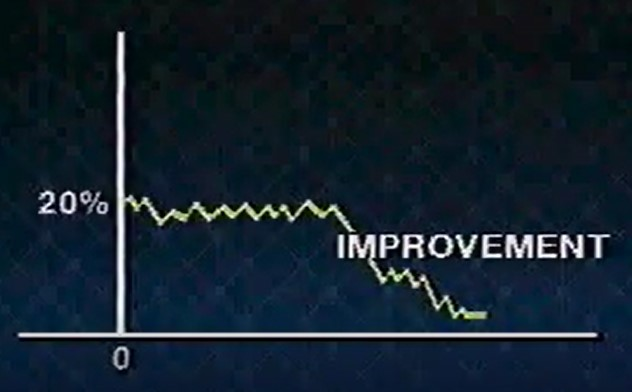
\includegraphics[width=10cm]{JuranImprovementScreenshot_2022-10-23_211444.jpg}

过程改进的计划一般包括:

\begin{enumerate}
\tightlist
\item
  如何识别选择项目。
\item
  组织改进项目的项目团队
\item
  找出缺陷根因
\item
  制定改进措施
\item
  验证是否在真正操作环境里面有效
\item
  处理团队文化上面的抗击阻力
\item
  控制保持本来的水平\\
\end{enumerate}

%\href{文件:IntroXPnJuranStepsScreenshot_2022-10-27_194505.jpg}{550px}

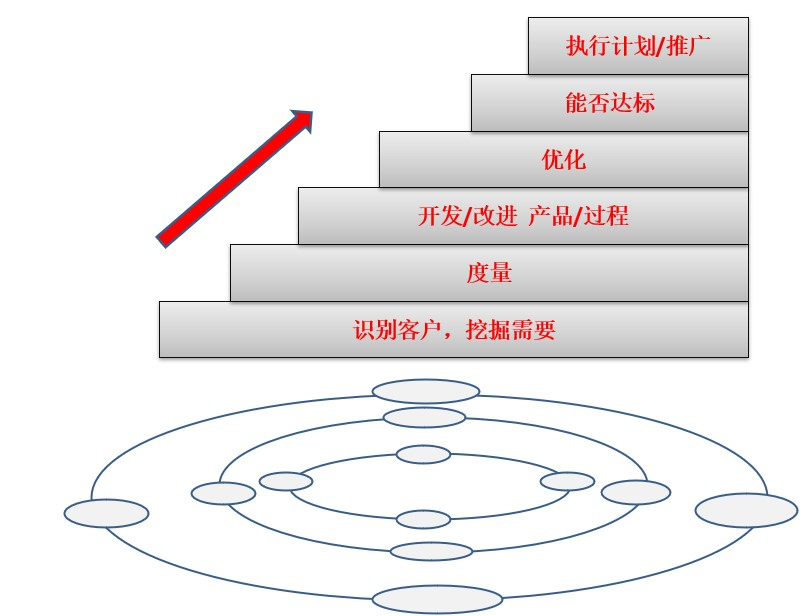
\includegraphics[width=10cm]{IntroXPnJuranStepsScreenshot_2022-10-27_194505.jpg}

客户:你说的策划、控制、改进都挺有道理,但如何跟敏捷,尤其是你说极限编程的实践关联呢?\\
我:任何最佳实践,如果没有定质量目标,配上度量衡量和策划,都只是空想,对长远提升公司文化、团队成员的习惯没有任何帮助。举例:参照上图,例如我们想改善团队的策划和估算。首先要识别客户,哪些是主要干系人
-
甲方有什么要求;内部部门经理,有什么要求。然后从他们的诉求变成过程的功能和特征,但如果特征只是描述,没有数字也没有意义,所以要配合可衡量的度量单位,和用什么方式去收集那些数字,然后依据目标定过程要怎么去做,怎样改。例如

\begin{itemize}
\tightlist
\item
  是否应该从本来的瀑布策划方式制定大的总计划,改用精益的思路,分成迭代,
\item
  每次估算应该怎么做、如何监控等
\item
  然后改进的过程要不断从实验中优化
\item
  最后还要用数字证明这改善比本来好,然后在其他团队全面推广\\
\end{itemize}

而不是单纯`空降'某敏捷流程(例如 SCRUM),便能加快团队的发布速度。
所以虽然极限编程里每一条实践都是最佳实践,也必须配合质量策划,和监控改进才会有效果。

\framebox{%
\begin{minipage}[t]{0.97\columnwidth}\raggedright
很多人都知道戴明环代表PDCA(Plan-Do-Check-Act),其实持续改进的道理也不是戴明博士发明,Juran
对它的了解与应用不会比戴明差。\strut
\end{minipage}}

要注意在整个过程里,高层起非常关键的作用:\\
所以Dr
Juran强调高层不能把公司的质量工作下放(例如,由某助手负责)。我们的经验就是这种做法往往导致最后质量不会有任何改进。原因很简单,每位中层管理者都有一定的KPI标准,资源也是固定的。如果这些没有根本的改变,质量是不会提升,因为整个管理环境没有变化,项目经理、部门经理还是会按以前的做法继续操作,不会听高层的口号或宣传,很快整个质量改进将会失败而终,所有的活动尤其质量相关的,高层必须亲身参与。包括制定质量目标,参与质量提升的高层委员会,定期监督进展等。

这手册会:

\begin{itemize}
\tightlist
\item
  先从个人如何提升,与自我管理开发过程开始
\item
  然后以团队如何做好迭代回顾(复盘)为改进试点\\
\end{itemize}

利用实际案例让大家了解如何开展过程改进。\\
然后,针对每条XP实践,探索如何能在团队里用上,并能改善开发产品的质量(降低客户缺陷密度)。\\
改进都要有衡量才具体,``度量与分析''部分会从基础概念开始,探索如何建立标杆(基线)与预测模型。\\

\hypertarget{ux9644ux4ef6}{%
\section{附件}\label{ux9644ux4ef6}}

\hypertarget{xp}{%
\subsection{XP}\label{xp}}

\hypertarget{ux7f16ux7801ux5b9eux8df5-coding-practices}{%
\subsubsection{编码实践 Coding
Practices}\label{ux7f16ux7801ux5b9eux8df5-coding-practices}}

\hypertarget{cp1ux7b80ux5355ux5730ux7f16ux7801ux548cux8bbeux8ba1-code-and-design-simply}{%
\paragraph{CP1:简单地编码和设计 Code and Design
Simply}\label{cp1ux7b80ux5355ux5730ux7f16ux7801ux548cux8bbeux8ba1-code-and-design-simply}}

\begin{itemize}
\tightlist
\item
  To produce software that is easy to change 使软件易于更改
\end{itemize}

\hypertarget{cp2ux65e0ux60c5ux5730ux91cdux6784-refactor-mercilessly}{%
\paragraph{CP2:无情地重构 Refactor
Mercilessly}\label{cp2ux65e0ux60c5ux5730ux91cdux6784-refactor-mercilessly}}

\begin{itemize}
\tightlist
\item
  To find the code's optimal design 找到代码的最佳设计
\end{itemize}

\hypertarget{cp3ux5236ux5b9aux7f16ux7801ux6807ux51c6-develop-coding-standards}{%
\paragraph{CP3:制定编码标准 Develop Coding
Standards}\label{cp3ux5236ux5b9aux7f16ux7801ux6807ux51c6-develop-coding-standards}}

\begin{itemize}
\tightlist
\item
  To communicate ideas clearly through code 通过代码清晰地传达想法
\end{itemize}

\hypertarget{cp4ux5171ux540cux7684ux8bcdux6c47-develop-a-common-vocabulary}{%
\paragraph{CP4:共同的词汇 Develop a Common
Vocabulary}\label{cp4ux5171ux540cux7684ux8bcdux6c47-develop-a-common-vocabulary}}

\begin{itemize}
\tightlist
\item
  To communicate ideas about code clearly 清楚传达软件设计的想法
\end{itemize}

\hypertarget{ux5f00ux53d1ux5b9eux8df5-develop-practices}{%
\subsubsection{开发实践 Develop
Practices}\label{ux5f00ux53d1ux5b9eux8df5-develop-practices}}

\hypertarget{dp1ux6d4bux8bd5ux9a71ux52a8ux5f00ux53d1tdd-test-driven-development}{%
\paragraph{DP1:测试驱动开发TDD
Test-Driven-Development}\label{dp1ux6d4bux8bd5ux9a71ux52a8ux5f00ux53d1tdd-test-driven-development}}

\begin{itemize}
\tightlist
\item
  To prove that code works as it should 来证明软件正常工作:\\
\end{itemize}

\begin{description}
\tightlist
\item[]
- Test-first programming(prim practice\#)
\end{description}

\hypertarget{dp2ux7ed3ux5bf9ux7f16ux7a0b-pair-programming}{%
\paragraph{DP2:结对编程 Pair
Programming}\label{dp2ux7ed3ux5bf9ux7f16ux7a0b-pair-programming}}

\begin{itemize}
\tightlist
\item
  To spread knowledge, experience and ideas 传播知识、经验和想法:\\
\end{itemize}

\begin{description}
\tightlist
\item[]
- Pair Programming(prim practice\#)
\end{description}

\hypertarget{dp3ux96c6ux4f53ux8d1fux8d23ux5199ux597dux4ee3ux7801vs-ux53eaux987eux8651ux81eaux5df1ux7684ux4ee3ux7801-collective-code-ownership-vs-individual-own-code}{%
\paragraph{DP3:集体负责写好代码(vs 只顾虑自己的代码) Collective Code
Ownership (vs individual own
code)}\label{dp3ux96c6ux4f53ux8d1fux8d23ux5199ux597dux4ee3ux7801vs-ux53eaux987eux8651ux81eaux5df1ux7684ux4ee3ux7801-collective-code-ownership-vs-individual-own-code}}

\begin{itemize}
\tightlist
\item
  To spread the responsibility for the code to the whole team
  将写好代码的责任扩展到整个团队:\\
\end{itemize}

\begin{description}
\tightlist
\item[]
- Whole team(prim practice\#)

- Share code(corollary practice\#)
\end{description}

\hypertarget{dp4ux6301ux7eedux96c6ux6210-integrate-continually}{%
\paragraph{DP4:持续集成 Integrate
Continually}\label{dp4ux6301ux7eedux96c6ux6210-integrate-continually}}

\begin{itemize}
\tightlist
\item
  To reduce the impact of adding new features 降低添加新功能的影响:
\end{itemize}

\begin{description}
\tightlist
\item[]
- Incremental Design(prim practice\#)

- Single code base(corollary practice\#)

- Ten-minute Build(prim practice\#)

- Continuous Integration(prim practice\#)
\end{description}

\hypertarget{ux5546ux52a1ux5b9eux8df5-business-practices}{%
\subsubsection{商务实践 Business
Practices}\label{ux5546ux52a1ux5b9eux8df5-business-practices}}

\hypertarget{bp1ux5c06ux5ba2ux6237ux6dfbux52a0ux8fdbux56e2ux961f-add-a-customer-to-the-team}{%
\paragraph{BP1:将客户添加进团队 Add a Customer to the
Team}\label{bp1ux5c06ux5ba2ux6237ux6dfbux52a0ux8fdbux56e2ux961f-add-a-customer-to-the-team}}

\begin{itemize}
\tightlist
\item
  To address business concerns accurately and directly
  准确、直接地解决业务问题:
\end{itemize}

\begin{description}
\tightlist
\item[]
- Real Customer involvement(corollary practice\#)
\end{description}

\hypertarget{bp2ux8ba1ux5212ux6e38ux620f-play-the-planning-game}{%
\paragraph{BP2:计划游戏 Play the Planning
Game}\label{bp2ux8ba1ux5212ux6e38ux620f-play-the-planning-game}}

\begin{itemize}
\tightlist
\item
  To schedule the most important work 安排最重要的工作:\\
\end{itemize}

\begin{description}
\tightlist
\item[]
- Weekly cycle ; Quarterly cycle ; Slack (prim practice\#)
\end{description}

\hypertarget{bp3ux5b9aux671fux53d1ux5e03-release-regularly}{%
\paragraph{BP3:定期发布 Release
Regularly}\label{bp3ux5b9aux671fux53d1ux5e03-release-regularly}}

\begin{itemize}
\tightlist
\item
  To return the customer's investment often
  尽早交付,让客户看到投资回报:
\end{itemize}

\begin{description}
\tightlist
\item[]
- Incremental Deployment(corollary practice\#)

- Daily Deployment(corollary practice\#)
\end{description}

\hypertarget{bp4ux4ee5ux53efux6301ux4e45ux7684ux901fux5ea6ux5de5ux4f5c-work-at-a-sustainable-pace}{%
\paragraph{BP4:以可持久的速度工作 Work at a Sustainable
Pace}\label{bp4ux4ee5ux53efux6301ux4e45ux7684ux901fux5ea6ux5de5ux4f5c-work-at-a-sustainable-pace}}

\begin{itemize}
\tightlist
\item
  To go home tired, but not exhausted 回家时虽然很累,但不筋疲力尽:\\
\end{itemize}

\begin{description}
\tightlist
\item[]
- Slack (prim practice\#)
\end{description}

\hypertarget{ux4e54ux5e03ux65afux8c08dr.juran}{%
\subsection{乔布斯谈Dr.Juran}\label{ux4e54ux5e03ux65afux8c08dr.juran}}

\framebox{%
\begin{minipage}[t]{0.97\columnwidth}\raggedright
他(NEXT CEO)接受访谈时,对美国企业,质量,和 Dr.Juran
观点的重点内容:\\
美国已经富裕了很多年。很多企业都忘记要获得成功,还是要关注基本功,包括教育。现在我们美国很多企业面临困难,处处感觉被日本领先了。其实不是日本针对我们,而是我们作为美国企业家应反思一下,为什么我们的战略比他们差,为什么我们的策划不如日本?我们知道Dr.Juran
在40/50年代多次去日本,帮助日本企业提升质量。现在他回到美国,希望把他的经验带到美国企业,提升竞争力,可以再一次成为世界第一。

我觉得Dr.Juran
很实在,不是泛泛而谈。我们的工程师也深受他这种风格影响。无论我们之中谁问他问题,总裁还是工程师,他都会全心全意用自己的知识解答。所以工程师和我都很希望用他那套方法来做提升。整个质量提升的道理其实很简单,是一个重复的过程,然后我们需要不断去看,有哪些无效的环节要省略,哪部分要重新设计,不断试验、提升,就这么简单。重点是所有的提升都应该是科学化的,有数据而不是泛泛而谈。

一般管理层的思路是:我是领袖,你们应该听我命令。但应该是反过来,让应如何做好的决定权利放在团队手上,做改进不需要请求管理层的批准。改进是工作的一部分,整个架构扁平化,自己管控日常过程,每位工程师应像以前的工匠,愿意花精力不断做好。然后能以自己最后做出的优质工艺、产物自豪。\strut
\end{minipage}}%done-1


\part{个人提升}自我改善效率基本功\\

%\part{个人提升\\ \textbullet \textbullet \textbullet \\自我改善效率基本功}

%

\chapter{如何创新} % Introduction chapter suppressed from the table of contents


今天在书店看到这本 ------ 张萌写的 ``人生效率手册''

\hypertarget{ux76eeux5f55ux8282ux9009}{%
\subsubsection{目录节选}\label{ux76eeux5f55ux8282ux9009}}

\begin{itemize}
\tightlist
\item
  目标建立
\item
  时间管理

  \begin{itemize}
  \tightlist
  \item
    有了目标才能开启时间管理之门
  \item
    把大目标分解成小目标,各个击破
  \end{itemize}
\item
  高效学习

  \begin{itemize}
  \tightlist
  \item
    预习,实时学习到最后复习,才是完整的学习过程
  \item
    早起掌控自己的时间,你是时间主人
  \item
    充满正能量,在激励中不断前进
  \end{itemize}
\item
  修炼硬本领
\item
  自我输入与输出

  \begin{itemize}
  \tightlist
  \item
    自我输入输出的渠道,不仅仅是上课听讲
  \item
    孰能生巧后,你才能成为别人的师父
  \item
    写作也是一种输出
  \end{itemize}
\end{itemize}

这书从制定目标开始,然后教你一些提升方法(如时间管理,高效学习等等)。
虽然有很多可参考的技巧,但有很重要一点她没有提到 -
如何驱动人改变以往的习惯?减肥的道理方法,每个人都懂,但为什么还是这么多人体重超标?

例如上一章说到的极限编程里的最佳实践都能很好帮助提升开发质量,现在已经20多年了;\\
质量大师Dr Juran质量手册(Quality Control
Handbook)里面也有很多质量改进的经典,大部分也适用于软件开发,第一版距今也已经50年了;\\
所以不能说没有方法,但为什么很多软件开发团队今天还是有不少质量问题?

锻炼身体或提升编程开发能力也如此。没有明确追求的目标,没有动力,任何好方法都帮不了你。

\hypertarget{ux521bux65b0-creativity}{%
\subsection{创新 Creativity}\label{ux521bux65b0-creativity}}

创新能推动改进,提高生产率。 但创新不局限于软件工程。\\
例如,音乐 - 作曲家都要具备极高的创新能力。\\
Robert FRITZ 回忆到 ``60年代,当我在BOSTON Conservatory
学音乐作曲时,开始思考学的不应仅仅是对位、和音,而是音乐大师的创新过程''
他毕业后继续做音乐创作,一次参加创新专业人士聚会,包括作家、画家、音乐家、建筑师等,他发现这些人在针对本身专业的创作能力都很厉害,但都没有想到用他们的创新能力提升自己的生活。
他便开始举办培训课帮不同背景的人提升创新,让各个行业也可以学什么是创作/创新。几年后,他把创作的重点写成了一本书
(见 Reference 参考)。Robert FRITZ 在他的书中,以贝多芬为例,说明创作并非
problem
solving(解决问题),而是要有一个很高的目标/理想,然后不断地尝试比较,最终达到创作目的。

\hypertarget{ux521bux9020ux7684ux7cbeux795e-spirit-of-creating}{%
\subsection{创造的精神 Spirit of
Creating}\label{ux521bux9020ux7684ux7cbeux795e-spirit-of-creating}}

创作不是由他人驱使,而是出于自身创作的欲望,要做世界上最优秀的作品。作家觉得自己的创作有价值,会用很多的精力进行创作。创作者努力创作,最终希望自己的作品以后有自己的生命力,受后人赞赏。

贝多芬,他对音乐创作的远景 (VISION)------
希望创造前所未有的作品(他觉得当代的作品离这远景还差很远,甚至包括他老师海顿和音乐天才莫扎特的作品)。由这崇高的远景驱动,加上他自身的音乐演奏/作曲能力,不断突破,甚至耳聋也阻挡不了他的创作力(从25岁开始听力减退,到45岁已经完全失聪)。
回顾贝多芬的创作生涯:\\
%\url{文件:Bdf.png}



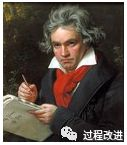
\includegraphics[width=10cm]{Bdf.jpg}\\

\framebox{%
\begin{minipage}[t]{0.97\columnwidth}\raggedright
\textbf{贝多芬} (1770 --
1827)的音乐创新可以说是前无古人后无来者,深深影响后面两世纪的作曲家。\\
我们都熟识他的命运交响曲,其实他从1795年到1827年去世前出版的每一首作品,无论是交响曲、室内乐、歌剧,都是经典。他是完美主义者,例如,田园交响曲(与命运同时出版与首演)的创作时间不少于3年,从他手稿得知,首乐章某主题他修改了不下12次,所以与莫扎特,舒伯特比较,他的``生产率''不算高,平均每年出版5\textasciitilde{}6个作品。

他出版命运、田园交响曲时(1808),已经出版音乐作品十三年,包括23首钢琴奏鸣曲,9首弦乐四重奏。
开始时,他与古典时期的海顿、莫扎特的风格类似,但是到了中期,如命运交响曲、田园交响曲,已经远远超出他前辈和同辈,启蒙音乐家从古典期发展成浪漫期新风格。

晚期的作品(如钢琴曲、弦乐四重奏等),又完全另一套与中前期不同风格。例如,他的Op133
弦乐四重奏 Große Fuge
由于思路远超于当时的水平,不被当时的音乐家接受,觉得作品有问题,有些甚至说他太老,不止聋了,并疯了。但贝多芬依然故我,说``这曲是为未来写的!''

他的音乐创作一直没有停下来,例如,他的最后弦乐四重奏(第16首)Op135在1826年出版。
贝多芬 一生写了32 首 钢琴奏鸣曲 ,
与莫扎特和他老师海顿不同,贝多芬每一首钢琴奏鸣曲虽然都是奏鸣曲式 (sonata
form),但都有独特创新,突破奏鸣曲式,变化万千。\strut
\end{minipage}}

他与其他音乐大师有一个共同的特点就是有把握自己命运,追求个人目标的主动心态,再加上本人的天赋、魄力,而非被动解决每天面对的问题
(Problem solving)。

远景 / 理想 /创意 我们大部分人都有,但为什么只有少数能成为大师?
所有创新都需要经过一个漫长的过程。

%\href{文件:liuct.png}{600px}
\includegraphics[width=20cm]{liuct.jpg}\\

\hypertarget{ux76eeux6807ux600eux6837ux8bbe-ux4ec0ux4e48ux6837ux7684ux76eeux6807ux624dux7b97ux7406ux60f3}{%
\subsection{目标怎样设?
什么样的目标才算理想?}\label{ux76eeux6807ux600eux6837ux8bbe-ux4ec0ux4e48ux6837ux7684ux76eeux6807ux624dux7b97ux7406ux60f3}}

妨碍个人或公司
提升的原因之一是觉得资源越多越好办事,现在很多事做不出来是因为资源不够


在杭州某商务酒店看到十几条写在墙上浙商名言,其中一条这么说:

%\href{文件:mingyant.png}{600px}
\includegraphics[width=13cm]{mingyant.jpg}\\
很多美国企业家也曾经是如此想,企业越大越稳固。但他们没有想到如果收购不能为公司带来增值,反而会使企业更脆弱。
个人要提升也不能这样想--`` 我现在能力 (资源)
不足,等我具备充分条件再说吧。''(如想知多些怎样能做到个人极限,可看附件
个人STRETCH的小建议)

丰田大野耐一 说得好 -- ``容易达成的目标不是好目标''
他对丰田员工设的质量目标是零缺陷!

%\href{文件:mubiaozhungt.png}{600px}
\includegraphics[width=13cm]{mubiaozhungt.jpg}\\
除了要对未来有一个远景 (VISION)
目标外,了解现状同样重要。但很多人`看'不到真正的,只`看'到自己想象的。

\framebox{%
\begin{minipage}[t]{0.97\columnwidth}\raggedright
很多画家不是画自己看到的,而是画他想象中的。一天画家带学生到美国新泽西州(New
Jersey)
写生,他指着远处3建筑物:山上的高层住宅;海边的仓库;河流上流的工厂。他问学生,这些建筑物什么颜色?所有学生都告诉他,住宅是红色、仓库是白色、工厂是橙红色。老师派给每个学生一张卡,卡上有一个小洞,小洞让学生只单独看到每个建筑物的一小部分,然后老师再问,现在你看到的什么颜色?
本来没有回应,有个学生说,所有都是蓝色,跟那些整个背景一样,本来那些建筑看起来都是蓝色。你可以想象当你在一个有雾的天,你看远处的山、河流、长街。因为我们中间有个大气层,空气,大气会反射光线,就是天空的光,会导致山看起来是蓝色、紫色。
所以当学生不被建筑物的影响下看颜色时,他才会看到真正的颜色。这个故事说明了,很多时候我们以为看到的不是一个真正的事实。\strut
\end{minipage}}

当管理者天天面对团队,但没有客观的数据,他不会感觉项目质量有问题。

开发团队大部分的缺陷都是在系统测试才被发现。
软件缺陷,越往后发现,返工量就越大。如果能在前面代码扫描,代码评审,单元测试等预先发现,
便可以大大减少返工工作量。\\
例如:项目两百多个系统测试缺陷
引起的返工量可能占总工作量三成以上,但因没有收集数据,大家都已经习惯了。\\
当企业有客观数据时,跟刚才那些学生看一些远景的真正颜色一样,他才知道真正样貌,这对整个公司的改进很重要,我们不仅仅是要定目标,更重要是要真正了解现状,才能感觉到差距,驱动改进,认知有差距,有动力做提升
-- 改变原来的习惯,开始动起来。

\hypertarget{fritz-ux628aux8fd9ux6539ux53d8ux8fc7ux7a0bux7b80ux5355ux5206ux4e3aux4e09ux6b65}{%
\subsection{FRITZ
把这改变过程简单分为三步}\label{fritz-ux628aux8fd9ux6539ux53d8ux8fc7ux7a0bux7b80ux5355ux5206ux4e3aux4e09ux6b65}}

\begin{enumerate}
\tightlist
\item
  Germination 萌芽
\item
  Assimilation 吸收
\item
  Momentum 动力
\end{enumerate}

萌芽是开始动起来,但我觉得中间的 吸收(Assimilation) 阶段
最关键好比我们学骑单车,学游泳,学帆船,如果可以过了这关键阶段,便可持续变为动力,成为常态。

FRITZ 刚进音乐学院开始跟老师上单簧管课,每周老师会给他练习曲,叫他去练 /
准备。第一周的曲子很难,他吹得不好。他本以为老师会叫他从练这曲子但老师接下来第二周挑选另一首比第一周更难的曲目,他第二周也吹不好一直这样。他连续练了六首越来越难的练习曲

过了六周后老师请他再吹第一周的曲子,他很轻松地便把它吹完,吹得比第一次好多了,也没有什么错误,然后老师要他在吹第二周的曲子结果也类似。作者对
assimilation 阶段 的经验教训:

\hypertarget{ux7ee7ux7eedux4e0bux4e00ux6b65ux662fux5e2eux4f60ux6d88ux5316ux73b0ux5728ux8fd9ux6b65ux7684ux6700ux4f73ux65b9ux6cd5}{%
\subsubsection{继续下一步是帮你消化现在这步的最佳方法。}\label{ux7ee7ux7eedux4e0bux4e00ux6b65ux662fux5e2eux4f60ux6d88ux5316ux73b0ux5728ux8fd9ux6b65ux7684ux6700ux4f73ux65b9ux6cd5}}

One powerful way to assimilate your present step is to move on to your
next step

回顾我开始写分享文章时,
虽然很困难,写不好,但我继续尝试慢慢变成习惯。起初只是一些零散的笔记,后面逐渐有主思路,有连贯性。如果可以从远景(vision),经过萌芽,吸收,便可以变成动力(momentum),
成为新的习惯。

\hypertarget{ux5fc3ux4ebaux5408ux4e00}{%
\subsubsection{心人合一}\label{ux5fc3ux4ebaux5408ux4e00}}

要改变以往的习惯(解冰),促进创新与提升,人体也要配合起来:

\framebox{%
\begin{minipage}[t]{0.97\columnwidth}\raggedright
Tips个人解冰 

我爱人是公立医院的物理治疗师,他知道运动对人体健康很重要,他常常提醒我每天要起码半个小时的带氧运动,但我长期出差,一年住商务酒店的时间不少于10个月。开始的时候,因早上要9点前到达客户现场,时间不够,
只可以隔几天早上15分钟 跑跑步,跳跳绳。最多15分钟
然后逐步把跑步的距离目标定高一点,比如酒店附近的一个地标,来回距离有2公里,现在我每天早上基本可以达到每天半小时的运动量。人的生理状态和心理状态是相关的。所以开始天天做运动,是个人解冰的好开始。\strut
\end{minipage}}


\hypertarget{references}{%
\section{References}\label{references}}

1. Robert FRITZ, The path of least resistance for Managers\\
  %done-1
%\chapter{克服拖延症} % Introduction chapter suppressed from the table of contents


技术总监问:现在我遇到最大的难题就是如何提升下面技术人员的能力,如果他们全都是高手,我就很轻松了,但实际上最多只有三分之一,其他都是中低水平。您接触过这么多软件开发团队,有什么好方案?\\
我:可以先听听这故事:\\


= = = = = = = = = = = = = = = = = = = = =


%\href{文件:小李图.png}{400px}


\includegraphics[width=8cm]{小李图.png}

小李:你平常办公时间都一直都很忙,还可以腾出晚上和周末时间,
把客户遇到的问题,如何解决等,汇总成分享文章,每两周公众号发布,很厉害呀。\\
我:其实你也可以做到。要成为专业软件工程师,除了要学习软件工程相关的知识与技能外,
个人有没有高效率的习惯其实更重要。

我在五年前教项目管理时参考过一本效率小册 {[}详见 Reference1{]},
这本小册罗列了99个小技巧,每个技巧都不超过一页纸,我自己也一直用这小手册提醒自己。

%\url{文件:超效率目录.png}

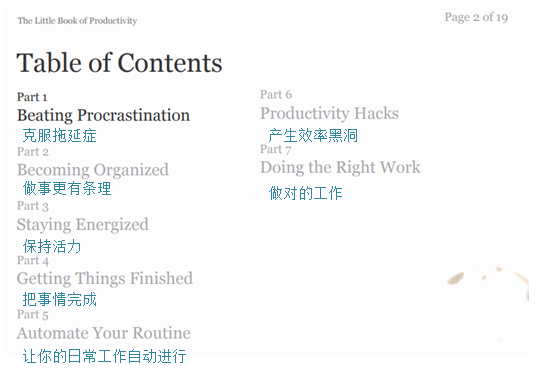
\includegraphics[width=10cm]{超效率目录.png}

例如,第一章``克服拖延症'',这里的几乎全部技巧有帮助:\\

\begin{itemize}
\tightlist
\item
  周 / 日目标 (1 Weekly / daily Goals)
\end{itemize}

\framebox{%
\begin{minipage}[t]{0.97\columnwidth}\raggedright
我每天都会定计划,早上希望完成哪些功能,下午完成哪些。当然这个计划也会按实际的进展调整。

周 /
日目标是个人时间管理的基本功。每一天第一件事不是回邮件,而是仔细想想今天要完成什么任务,每一周的开始,也应该想我本周希望完成什么任务。不然的话,每天的时间就很容易被琐碎的小事吃掉,一事无成。\\
\strut
\end{minipage}}

\framebox{%
\begin{minipage}[t]{0.97\columnwidth}\raggedright
背后的道理很简单, 要把时间花在重要、但非紧急的活动(下图右上角
)上,效率才会出来。

%\href{文件:紧迫非紧迫_3.0.png}{600px}\strut
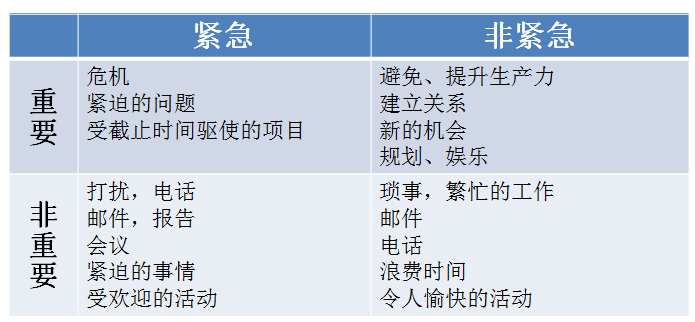
\includegraphics[width=10cm]{紧迫非紧迫30.png}
\strut
\end{minipage}}

\begin{itemize}
\tightlist
\item
  限定时间 (2 Timeboxing)
\end{itemize}

\framebox{%
\begin{minipage}[t]{0.97\columnwidth}\raggedright 把每天的任务安排成时间段,每一段不应超过1.5
小时。\strut 一般人可以专心集中的时间段都不会超过60分钟,小孩可能就更短。如果老师叫你星期五5点钟交卷,你不会3、4点就交,都会等到最后十分钟,甚至五分钟。所以如果我们把一天的时间切开成
1 ~ 1.5 小时时间段,自然有动力,
希望在时间之内完成任务。\strut 我们写代码的时候应该也是用同样的原理。例如。前面那个总共花了10个小时的功能,也是本身尝试了很多次。每次当我发现超过了1小时或者1.5
小时,我就会把它放下来,先做其他事。\strut
\end{minipage}}

\begin{itemize}
\tightlist
\item
  分解任务 (3 Dissolving tasks)
\end{itemize}

\framebox{%
\begin{minipage}[t]{0.97\columnwidth}\raggedright
因为都是练习题,所以每一个功能都比较细,不会超过二十行。如果我们平常做开发时,也必须要把一些大、复杂的功能预先拆分成小的功能才有效率。\strut
\end{minipage}}

\begin{itemize}
\tightlist
\item
  加强自律 (6 Building Self-Discipline Muscles)
\end{itemize}

\begin{description}
\tightlist
\item[]
晨礼(30 Morning Rituals) 日常运动 (32 Make an Exercise Routine)
\end{description}

\framebox{%
\begin{minipage}[t]{0.97\columnwidth}\raggedright
不要以为编码是一个单纯的脑力活。整天坐在电脑前面敲代码就可以,如果人的体力、精力没有配合上也会出问题,好在我每天早上一直坚持三十到四十分钟的轻量运动,然后晚饭前半个小时到一个小时的骑单车或者慢跑的习惯。中间也是不是整天坐着,一段时间会走一走,喝橙汁等,确保身体不断在动,才不会困,保持动力。

贝多芬每天都会去外面散步,来启发一些创作的灵感,然后他会立马把这些写在本子上,用于后面的音乐创作。早上的跑步也可以让我有多些创作灵感。\strut
\end{minipage}}

\begin{itemize}
\tightlist
\item
  不会分心的工作场所 (11 Create a Distraction-Free workplace)
\item
  轻策划,迭代,再策划 (13 Ready , Fire, Aim!)
\end{itemize}

\framebox{%
\begin{minipage}[t]{0.97\columnwidth}\raggedright
三十年前,软件开发都是很大型的一些项目,整个架构要设计好才动手去写代码。现在反过来,需求变化极大,开发都需要敏捷,轻文档轻计划。尽快写好代码,做一些功能给客户,从反馈优化下一轮。我这次的几天开发也是用同样原则,没有花时间在一些设计或者文档。想直接把那个代码写出来,并通过单元测试,就节省很多耗时间的工作。把有限的时间都放在写好代码上。\strut
\end{minipage}}

\begin{itemize}
\tightlist
\item
  不断清洗 (10 Churning)
\end{itemize}

\framebox{%
\begin{minipage}[t]{0.97\columnwidth}\raggedright
万事开头难。我在开始的半天也是遇到同样问题,不知如何入手,太久没看写代码的书了,很多基本的都不知如何入手。所以我开始的时候不会直接尝试写题目里面的功能,而是重写一些书本的代码,看看跑出来怎么样,然后逐步提升。写一些基本功能,慢慢有了习惯,调整过来了,后面就越来越顺。好比一台旧的水泵,刚开始抽上来的水总是有难喝的铁锈,只要不停止抽水,当污水最终都从系统中抽出后,就能发现底下的净水。\strut
\end{minipage}}

\begin{itemize}
\tightlist
\item
  要有好的土壤 (8 Remove your Hidden Roadblocks)
\end{itemize}

\framebox{%
\begin{minipage}[t]{0.97\columnwidth}\raggedright
在含盐量高的土壤里种植物,是结不出果实的。浇水、平衡在阴凉处和阳光下的时间都抵不过根部吸入的毒素。如果我们没有积极性,就可能是土壤的问题。如果没有足够的积极动力,就不会在长假专注写程序,也不会定期要求自己写分享文章。所以要有明确/很想达到的目标驱动。
像一个作曲家,他希望写出很多经典的优秀作品,不满足于现在的状态。觉得自己的灵感或者创造力没有发挥出来,成为可以保留下来的东西。也是这种驱动力让我可以一直努力做这件事。\strut
\end{minipage}}

\begin{itemize}
\tightlist
\item
  摒弃拖延恶习 (14 Quit your Procrastination Vices)
\end{itemize}

\framebox{%
\begin{minipage}[t]{0.97\columnwidth}\raggedright
长假里,大部分人都会把时间用于看视频或电视剧,而我正好没有这个习惯,也一直没有玩网络游戏的习惯,否则肯定完成不了。\strut
\end{minipage}}

最终我用日程记录(91
Timelogging),把整件事和什么活动、时间花在什么地方都记录下来了。

小李:我看你上面列出的技巧,我大部分都还没做到。

我:不要紧,我六年前刚开始定期写文章时情况跟你类似,但只要不放弃,一直往既定目标努力,不良习惯都改正过来了。

我常常说人的潜力是极大的。 舒伯特你听过吗?\\
小李:好像是一个很有名的作曲家。\\
我:是的,但他很年轻31岁(1828)
就去世了,你猜他一生一共写了多少首歌和音乐作品。\\
小李:我记得中学时,老师介绍过他的艺术歌曲,如``鳟鱼 The
Trout'',但他31岁就死了,我猜100 - 200 首歌?\\
我:他一生写了超过460首歌曲(时长\textgreater{}24小时)。除了歌曲,他还写了其他作品,如9首交响曲,20
室内乐,120 钢琴曲等等,每一类都包括大量经典作品,对后世影响深远。\\
小李:如果粗算他一生600作品,算他有16年时间作曲,平均每月要完成3个作品,真是不得了。\\
我:虽然他的作品有大有小(从一首歌,到45分钟的交响曲),他确实生产率极高,而且他最后的7年一直身体都不好,所以他那个时候肯定不会像我们现代996方式工作。
他每天主要是早上用来写作,傍晚便去休息散步。但他会同时做多个创作项目 -
那些项目没有灵感,就暂时放下来,创作其他作品。
他著名的未完成交响曲就是个好例子,只有两个乐章(一般交响曲都是四个乐章)
所以他是使用高效技巧的一个成功例子。

每个人都有自己的理想,但如果没有高效率来执行,理想只是天马行空,天方夜谭,不会有任何成就。有没有疑问?

小李:没有,挺好的,我后面立马就开始。\\
:: = = = = = = = = = = = = = = = = = = = = =\\
总监:我大概懂你的意思了,要提升技术人员的能力先要改变他们的习惯,有良好的习惯(如时间管理),才有机会提升。\\
我:是的。\\
总监:从管理者的角度,我们有什么可以做的?\\

\framebox{%
\begin{minipage}[t]{0.97\columnwidth}\raggedright
即时笔记 (17 The Capture Device)
总监边听边在本子上记下那些重点。高效的人都会有工具帮他记录想到灵感、想法、项目、待做事项等等,不会仅仅靠大脑记忆。你提出一个要求,他会立马写在小本子上,你会觉得他应该会按你要求去处理,但反过来他只是口头说会处理,你会担心很可能没有下文。但我看有些领导,身边只拿个手机,除非他们的记忆力超人,不然话我估计他每天都会忘记不少重要事项。\strut
\end{minipage}}

\hypertarget{ux676dux5ddeux9ad8ux7ea7ux7ecfux7406ux7684ux53cdux9988ux548cux9ad8ux89c1}{%
\subsubsection{杭州高级经理的反馈和高见}\label{ux676dux5ddeux9ad8ux7ea7ux7ecfux7406ux7684ux53cdux9988ux548cux9ad8ux89c1}}

人一定要自律!您说的小技巧确实能起到很大帮助,而且我基本都会使用,但如果不养成习惯,想起来使用下,最终还是改不了拖延症,所以要解决拖延症,一定从根源做起,还是得靠自己,需要培养自己意志力、专注力,坚持好习惯,改掉坏毛病。

\hypertarget{references}{%
\section{References}\label{references}}

1. YOUNG, Scott: "The Little book of Productivity"
(有中文翻译版,叫《超效率手册》 )\\




  %done-1


\part{自我管理开发过程}软件开发工程师自我改进过程\\

%\part{自我管理开发过程\\ \textbullet \textbullet \textbullet \\软件开发工程师自我改进过程}

%\chapter{三点估算} % Introduction chapter suppressed from the table of contents




%\chapter{PERT} % Introduction chapter suppressed from the table of contents



\hypertarget{ux4f30ux7b97ux662fux4e00ux4e2aux8303ux56f4ux4e0dux662fux4e00ux4e2aux6570}{%
\subsection{估算是一个范围,不是一个数}\label{ux4f30ux7b97ux662fux4e00ux4e2aux8303ux56f4ux4e0dux662fux4e00ux4e2aux6570}}

唐工:你估计要完成开发用户登录模块要多少天?\\
小李:三天。\\
唐工:能在三天完成的可能性有多高?\\
小李:可能性很高。\\
唐工:可否量化一点?\\
小李:估计50\%-60\%。\\
唐工:所以很有机会不止三天,要四天了。\\
小李:对的,其实也有可能甚至要五、六天,但我估计机会不大。\\
唐工:你信心有多少?\\
小李:难说,有95\%的信心可以在六天之内完成。\\
唐工:所以有可能甚至要用上七天了?\\
小李:这样说吧,如果所有可能出问题的都出了问题,甚至会10或11天,但这种概率很低。\\
(最终管理者唐工还是要求有一个承诺,而不是一个估算)\\
所以唐工再问小李:是能否给我一个确实能完成这个模块的日期?\\
小李:正如我前面说,很可能三天可以完成,但有可能四天。\\
唐工追问:你可以说四天吗?\\
小李:也有可能五六天。\\
唐工结束对话:OK,请你尽力六天之内完成这个模块。\\
唐工貌似请求,但实际是要求小李承诺这个模块要在六天之内开发完。假如这个模块的开发时间超过六天,唐工就有依据说小李没有尽力导致延误了。\\
所以从以上对话,可以看到作为开发专业人员,必须分清估算和承诺。作为专业人士,我们不应该给一些没有把握的承诺,误导对方。中国老话说一诺千金就是这个道理。

\hypertarget{ux4eceux5355ux70b9ux52303ux70b9ux4f30ux7b97}{%
\subsection{从单点到三点估算}\label{ux4eceux5355ux70b9ux52303ux70b9ux4f30ux7b97}}

从上面的例子可以看到,一般的单点估算是很容易被误导,以为那个天数是有把握达成的,所以我们最好从单点估算变成三点估算,除了估算最可能的天数,还有最佳和最差共三点。但项目是由一系列的任务组成(如第二任务依赖于第一个任务的完成),如何计算所有任务的总天数?
下面用例子说明如何用3种使用三点估算估计的方法(A,B,C)估算总天数:\\
A) 假定都是正态分布,用模型估计:\\
先用PERT方程式计算每一步的预计值 与 标准差:\\
预计值 Expected Value EV = (Best + 4xMost Likely + Worst ) /6\\
标准差 Sigma= (Worst - Best) / 6\\

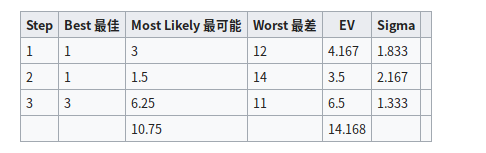
\includegraphics[width=6cm]{Screenshotfrom20221215004629.png}

如果假定是正态分布,按以上预计值和标准差,使用蒙地卡罗模拟,从下图可看到,95\%范围是
8.02 \textasciitilde{} 20.37\\
%\url{文件:pert3.1.png}

\includegraphics[width=6cm]{pert31.png}

B) 直接用PERT方程式计算总天数的均值与标准差:\\
如不用模拟,直接把3步的均值加起来\\
4.2 + 3.5 + 3.6 = 14\\
计算3步总方差:(方差 = \(Sigma^2\))\\
假定: 总方差 = 每步方差的总和\\
总方差 = 9.77\\
Sigma \(\sigma\)= 3.13\\
95\%范围计算公式为:均值的总和
\(\pm 2 \sigma = (4.2 + 3.5 + 3.6) \pm 2 x 3.13  = 14 \pm 6.26\)= 7.74
\textasciitilde{} 20.26\\
结果与蒙地卡罗模拟预测类似。\\
C) 假定都是三角形分布,用模型估计:\\
如果用三角形分布,95\%范围是 10.38 \textasciitilde{} 26.45\\
%\url{文件:pert3.2.png}

\includegraphics[width=6cm]{pert32.png}

\hypertarget{ux603bux7ed3-ux89e3ux8bfbux5206ux6790ux7ed3ux679c}{%
\subsection{总结 +
解读分析结果}\label{ux603bux7ed3-ux89e3ux8bfbux5206ux6790ux7ed3ux679c}}

\begin{itemize}
\tightlist
\item
  如果假定每一步的分布都是一个正态分布,就可以用头两个方程式计算每一步的平均值跟标准差和方差,用方程式可计算3步的总均值大概是14。也可以用方程式计算标准差,总的sigma
  (标准差)是3.13左右。
\item
  也可用蒙地卡罗模型(假定步骤都是正态分布),得出很类似的正态分布,总的平均也接近14,95\%的范围是从8.02到20.37,
  接近上面算出的均值 \(\pm\) 两个标准差数值。
\item
  但因三个步骤都是明显往右偏,所以不能假设它们是正态分布,更合适的是使用三角形分布,然后用蒙地卡罗估算``加''起来的分布,看见最后一个图明显是类似往右有个尾巴,能更正确反应三个步骤加起来的天数的估计分布。
\item
  跟假定正态分布的结果比较,很明显看到用三角形分布结果往右偏,上限是
  26.45(比正态分布的20.37
  高)。不是正态分布的话,左面就没有长尾巴,所以就会比本来正态分布的下限高,下限是
  10.38 (比正态分布的 8 高)。
\item
  从这简单例子看到,如果我们要把三点估算加起来,尤其是非正态分布的话,就不能用简单的方程式,或者假定它是正态分布来计算,需要用蒙地卡罗模型假设三角形分布才能能真正反应总体的分布。\\
\end{itemize}

从这三个偏左分布步骤例子看起来好像有些偏差,但不是很严重。如果我们看见用十个步骤都是偏一边分布,总分布会如何?是否相差会更远?

\hypertarget{ux5229ux7528ux8499ux5730ux5361ux7f57ux6a21ux62df10ux4e2aux6b65ux9aa4ux4e09ux89d2ux5f62ux5206ux5e03ux7684ux603bux5206ux5e03}{%
\subsection{利用蒙地卡罗模拟10个步骤(三角形分布)的总分布}\label{ux5229ux7528ux8499ux5730ux5361ux7f57ux6a21ux62df10ux4e2aux6b65ux9aa4ux4e09ux89d2ux5f62ux5206ux5e03ux7684ux603bux5206ux5e03}}

如果每步都估算天数,10个步骤的 总天数就是500天 (把10个估算值加起来)。

但如果每个步骤都是三点估算:

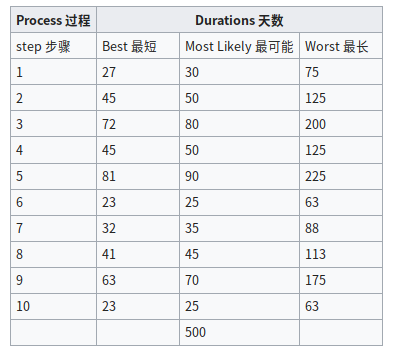
\includegraphics[width=6cm]{Screenshotfrom20221215004743.png}

很明显看到每一步都是偏左的分布,所以可预计总天数应不止500天,
但估多少才合适?

假定每步骤是三角形分布,用模型估计,重复五千次,得出下面分布:

%\href{文件:HMTT_v1.3_s77.png}{400px}

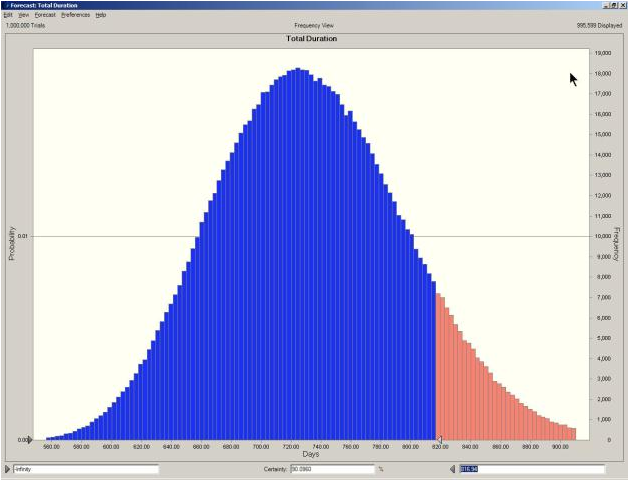
\includegraphics[width=6cm]{HMTTv13s77.png}

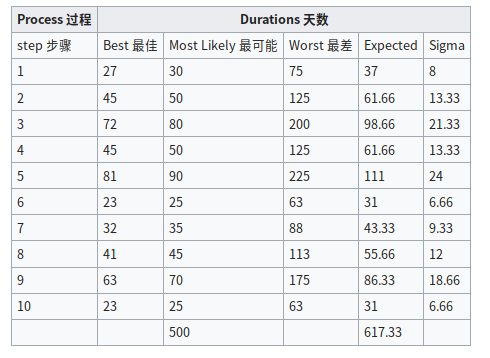
\includegraphics[width=6cm]{Screenshotfrom20221215004901.png}

A) 用PERT方程式计算每一步的预计值 与 标准差:

%\href{文件:10stepsPertScreenshot_2022-10-24_205007.jpg}{500px}

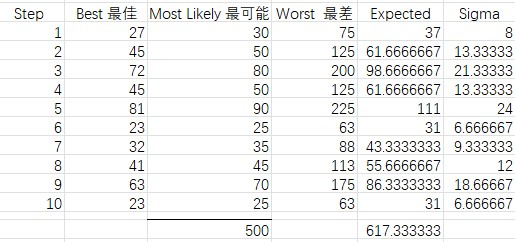
\includegraphics[width=6cm]{10stepsPertScreenshot20221024205007.jpg}

假定是正态分布,按以上预计值和标准差,使用蒙地卡罗模拟,得出的总分布与上面用三角形分布的结果几乎一致,都是左右平均分布的正态形。

\hypertarget{ux5206ux679010ux6b65ux9aa4ux6a21ux62dfux7ed3ux679c}{%
\subsection{分析10步骤模拟结果}\label{ux5206ux679010ux6b65ux9aa4ux6a21ux62dfux7ed3ux679c}}

\begin{itemize}
\tightlist
\item
  为什么用三角形模拟出来不是偏左的分布(类似前面3步结果),而是一个正态分布
\end{itemize}

\begin{description}
\tightlist
\item[]
以上实验验证了``中心极限定理'',无论本来是什么形状的分布,如果随机抽样够多,样本的平均值分布接近正态分布。所以如果本来只是三个步骤的时候还是可以看出是三角形偏左,但到了用十个步骤相加的时候,就跟每个都是用正态分布去估算的结果没有什么区分。\\

(中心极限定理会在后面数据分析里用上,例如通过画控制图判断过程是否稳定)\\
\end{description}

\begin{itemize}
\tightlist
\item
  实验结果也验证了PERT三点估算法公式,无论任何分布都可以用PERT公式计算每一步的预计值和标准差,然后计算总结果的分布(不需要蒙地卡罗模拟),当步骤越多差异就越小,如果是像上面的例子,只是希望求十个步骤的总分布(无论每步本身是怎样分布),都不需要用模拟,用PERT公式计算便可。\\
\end{itemize}

\begin{description}
\tightlist
\item[]
(这不表示蒙地卡罗模型没有用,到后面根因分析部分,我们还是会继续用它来比较不同的搭配选择最优)
\end{description}

\hypertarget{ux9644ux4ef6}{%
\section{附件}\label{ux9644ux4ef6}}

\hypertarget{ux8499ux5730ux5361ux7f57monte-carlo-ux6a21ux62df}{%
\subsection{蒙地卡罗(Monte Carlo)
模拟}\label{ux8499ux5730ux5361ux7f57monte-carlo-ux6a21ux62df}}

当结果不能用数学公式计算的时候(例如是三角形分布),可以用电脑随机模拟结果。例如:

\begin{itemize}
\tightlist
\item
  计算三个步骤的总共人天,每个步骤都是三角形分布,我们就用电脑的随机功能模拟,让随机功能的结果按三角形分布:
\item
  第一次模拟:步骤1得出1.3,步骤2得出1.2,步骤3得出2.0,得出三个步骤的总工期是4.5人天。
\item
  第二次 。 。 。
\item
  如果我们模拟1000次,10000次就有,便能模拟出总分布
\end{itemize}

5000次

%\href{文件:捕获2-1.PNG}{500px}

%\href{文件:捕获2.PNG}{500px}

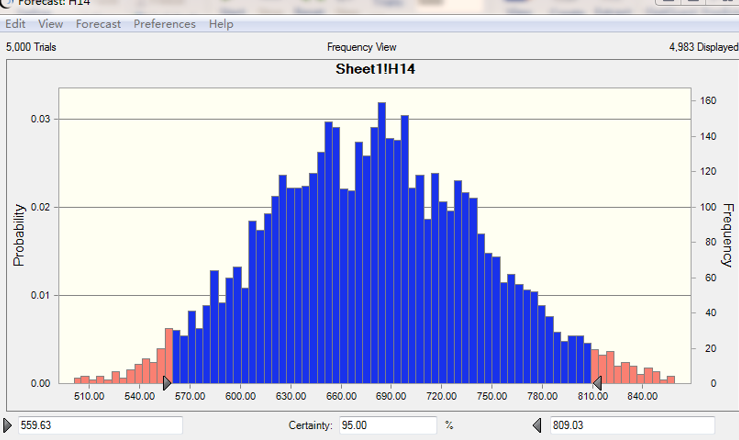
\includegraphics[width=6cm]{捕获21.PNG}

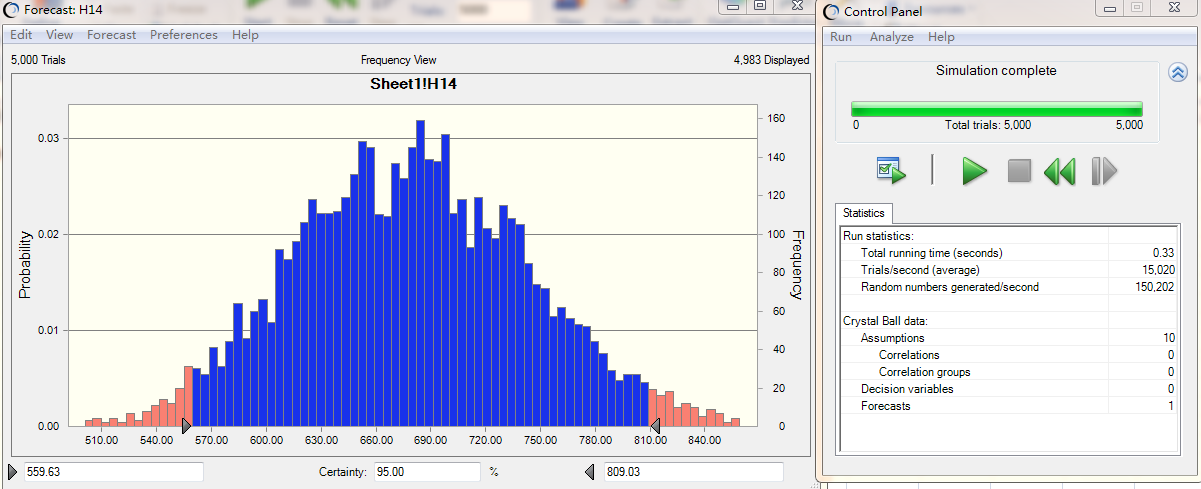
\includegraphics[width=6cm]{捕获2.PNG}


10000次

%\href{文件:捕获1-1.PNG}{500px}

%\href{文件:捕获1.PNG}{500px}

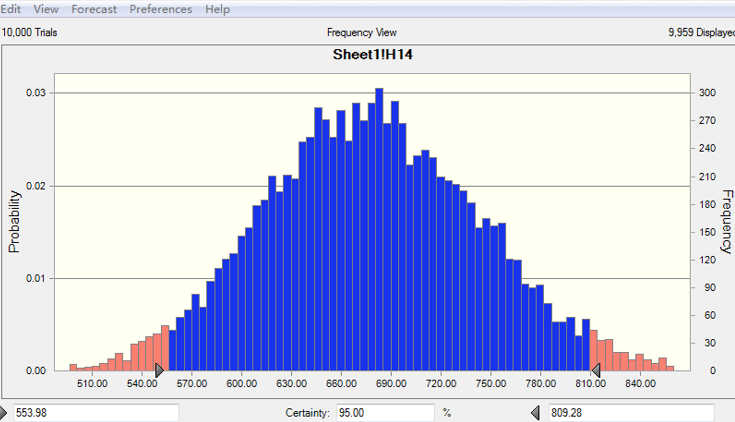
\includegraphics[width=6cm]{捕获11.PNG}

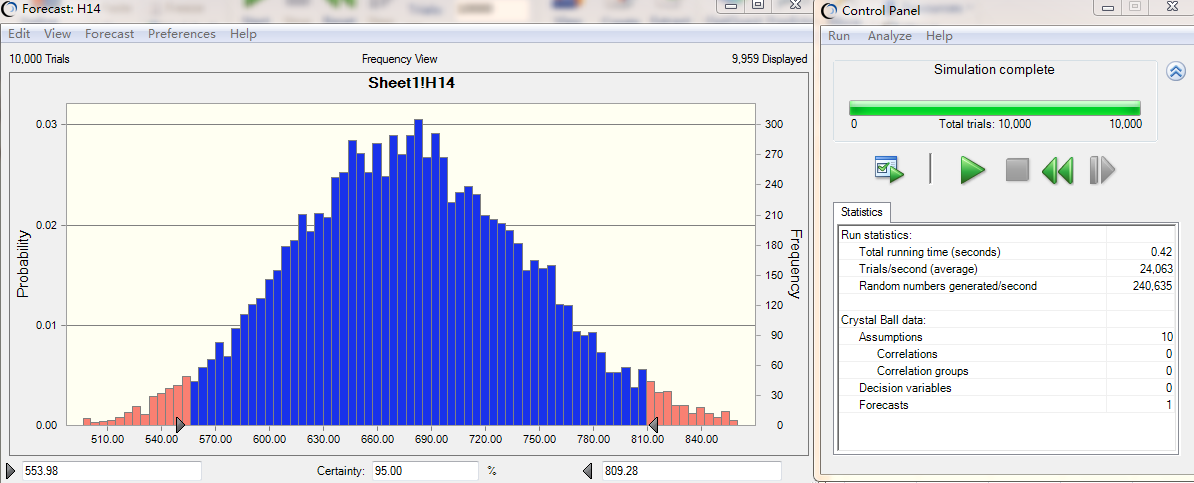
\includegraphics[width=6cm]{捕获1.PNG}





 %done-1
%\chapter{量化管理从个人开始} % Introduction chapter suppressed from the table of contents


\framebox{%
\begin{minipage}[t]{0.97\columnwidth}\raggedright
我:你们管理层和客户都比较关心项目的进度,项目是否能按时完成?请问你们过去的项目如何?\\开发:我们现在就是走敏捷开发,两周一个迭代。每次迭代前,我们聚一起开会,把所有用户故事按优先级排序,估计这个迭代可以完成哪些任务?然后放在看板的待办事项里。每天我们会做站立会议,监控实际的进展\\我:你们都能按计划在冲刺迭代里把所有任务开发好吗?\\开发想了一下,说:我们也有延误出现,有些模块不能在计划的冲刺里完成。\\我:为什么?\\开发:我们花了很多时间修正系统测试暴露的问题,有一些是因为前面没有把需求分析透导致的返工。\\我:请问你们是怎么估计每个任务应该花多少时间?\\ 开发:我们会一起讨论,然后用敏捷的扑克牌方式,集思广益,估计出来。\\ 我:除了你们每天站立会议监控项目的进展,你们要不要统计一下项目延期的水平是多少?\\开发:其实我们也不算是延误,有些模块不能在本迭代完成,就放在下一个迭代去做。\\ 我:软件开发有一个系数叫每人的生产率,就是开发人员一天能产出多少有效代码?你们有统计吗?\\开发:你说的是否是敏捷开发燃烧图里的速度(Velocity)?我们有画,但发现变化波动很大,所以后面我们也没有再用。\\ 
\strut
\end{minipage}}

\hypertarget{ux5982ux4f55ux964dux4f4eux9879ux76eeux8fdbux5ea6ux504fux5dee}{%
\subsection{如何降低项目进度偏差}\label{ux5982ux4f55ux964dux4f4eux9879ux76eeux8fdbux5ea6ux504fux5dee}}

从以上对话可以看到,敏捷开发不一定能帮助团队按期交付,开发人员也不清楚自己的生产率是多少。要减少项目的延误,首先取决于估算是否准确。但如果只是依赖个人经验、头脑风暴去估计,很可能低估,因为可能没有考虑开发以外的一些因素,比如缺陷问题、需求问题等等。在同一个冲刺里,不能交付所有计划的模块,等同于延误。要做好估算,就需要有数据。数据需要从个人从收集的历史数据作为参考。IT公司是否有注意这方面?我们可以从他们的新员工入职培训探索一下。

\framebox{%
\begin{minipage}[t]{0.97\columnwidth}\raggedright
我:请问你们如何培训新入职的开发人员?\\ 内部培训师:我们会先上一些基础的理论课,培训公司的代码规范、框架和复用的模块。然后进行个人或小组练习,我们会简化一些简单的开发项目里面的某个模块,让他们照着做个小项目,然后我们就会对他们的成果进行反馈,让他们知道自己的开发水平如何,是否掌握了我们所培训的内容。\\ 我:他们会收到什么反馈?\\培训师:理论培训后会有一些选择题考试,会出成绩。我们也会对他们做出来的程序打分。\\我:怎样打分?\\培训师:我们依据评判标准打分,分数从1-5,1最低,5最高。\\我:评判的标准可以说说吗?\\培训师:(想了一下)
依据他们是否掌握了培训内容的重点打分。\\我:你们公司不是已经开始推行量化项目管理,是否应该也配合量化管理,不仅仅靠老师主观判断打分?\\ 培训师:可否举些例子?\\我:例如他们质量方面的缺陷数,如果他们有做单元测试或者评审相关阶段的缺陷排除,项目管理相关所花费的工时,从而可以反算出来编码的效率等客观的量化指标。\strut
\end{minipage}}

\hypertarget{ux4eceux91cfux5316ux57f9ux8badux5f00ux59cb}{%
\subsection{从量化培训开始}\label{ux4eceux91cfux5316ux57f9ux8badux5f00ux59cb}}

从以上对话可以看出很多公司都没有与量化软件开发项目管理相关的培训,这样如何能希望他们在项目中做好量化管理?入职不仅需要培训开发的技巧、怎么写好程序、做好面向对象设计,也应该学到要一直度量自己的开发过程,包括所花的工时,过程中发现的缺陷数等。\\
培训师:在我们新员工培训时,如何可以加入这些量化的元素?\\
我:很简单。首先,在先培训质量相关的技术指标,比如什么叫质量成本,什么叫排除率等,然后做实战练习时,要求他们除了写程序,还需要记录一下所花的工时,自己项目走查时发现的缺陷数,测试的缺陷数,评审所花的时间等等。也要求开发人员除了提交程序以外,提交一个开发计划报告,内容包括实际所花工时,本来预估的工时,过程里发现得缺陷数,在哪一类过程等等。帮助他们一进入公司就培养一些量化度量的习惯,以避免过了试用期,开发的习惯已经养成,后面是很难改变的。\\

\hypertarget{ux4e92ux52a8ux57f9ux8bad}{%
\subsection{互动培训}\label{ux4e92ux52a8ux57f9ux8bad}}

举例:敏捷的小组传球游戏:\\
开头让人员传球,每做完一轮以后再估计下一轮的可以传多少个球。道理一样,让团队可以有据可依,更好地估计下一轮迭代。

本来这个传乒乓球的游戏,目的是让团队参考上一个迭代的数据,估计下一个迭代。但因为每个迭代开发的东西不一样,有些模块是复用的,有些是重新开发的,肯定所花的工作量不一样,所以虽然用以往经验估算下一个迭代概念上没有问题,但实际上可适用的场景很有限。如何可以帮团队做好估算与监控?可以看看我的亲身实验。

\hypertarget{ux4eceux4f30ux7b97ux7b56ux5212ux5230ux76d1ux63a7}{%
\subsection{从估算、策划到监控}\label{ux4eceux4f30ux7b97ux7b56ux5212ux5230ux76d1ux63a7}}

挣值分析(Earned Value EV)是常用的项目监控技巧,
没有项目管理工具也可以简单手动做用挣值分析。Humphrey先生出版了不少书,他都用EV分析来监控进度,他在PSP书中以此为实例,介绍了如何用挣值分析策划与监控。

%\href{文件:PSP_fig7.2.jpg}{350px}

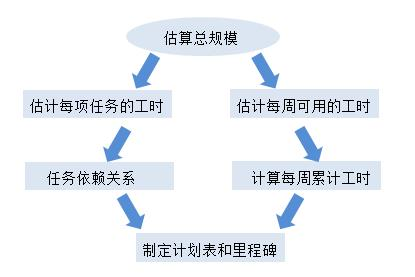
\includegraphics[width=10cm]{PSPfig72.jpg}

下面我也用同样思路来监控本书的进度:\\

\framebox{%
\begin{minipage}[t]{0.97\columnwidth}\raggedright
今天11月8日,离年底要交书的全部初稿给出版社时间不到两个月,书的内容也完成了超过一半,但剩下的时间因为年底密密麻麻很多评估,而且评估就是早上九点开始到下午五六点结束,只有中间一些空档时间和周末可以自由安排,所以我就用他的思路来策划估算是否能在年底完成要求。
第一步算出现在到年底可以用在写书的时间,按每周估计:

%\url{文件:psp3.jpg}

\includegraphics[width=10cm]{psp3.jpg}

第二步从历史的数据估算剩下的章节,每个章节需要多少小时,写出计划的完成顺序,然后依据原计划可以使用的每周时间,按最佳使用算出每个章节可以在哪周完成,写在表格的右面空白处,从而就可以估算出完成所有章节何时可以完成,如果确实不能到12月底完成,就可能要重新调整、策划,是否有一些章节优先级比较低,暂时不放在第一版。

因觉得单点估算很难定一个点数,便用三点估算法。每一行估计都有三点:最差、最佳、最可能,用
PERT方程式估计预计(Expected) 和 标准差(Sigma)。\\
:(实际顺序可能会有变,以上是已调整版本,原本 MGR 章节是放在后面。。。)

挣值析法所有东西 -- EV, PV, AC
都是用钱来结算(这个例子我们就是用所花工时),例如我们估计了每个章节所需要的工时,利用三点估算计算出每个章节预计的工时,加起来得出预计总工时是80.33工时(用PERT公式计算)。例如第一个章节TDD,预期工时是2.5,除以80.33就得出0.031,我们就用3.1作为TDD的PV(所有任务完成的总PV大概是100)。同样方式算出MGR章节的PV是6.6。(我本来也犯错,以为PV是和产出多少,或页数,成比例,但如用页数作为PV单位的话,就跟其它挣值分析法的系数,如EV,对不上了,导致错误。)得出每一个章节对应的PV后,我们就可以计算累计的PV数:

%\href{文件:psp1.1.jpg}{600px}

\includegraphics[width=10cm]{psp11.jpg}

估计哪一周可以完成哪些章节,得出总体的进度计划。例如第三周累积有66工时,应可完成总共12(=1+4+7)
个章节,因用PERT 三点估算,累积工时95\%范围是(55.8 \textasciitilde{}
62.5)(详见附件)。

%\href{文件:PSP3wksPlanScreenshot_2022-11-26_085813.jpg}{600px}

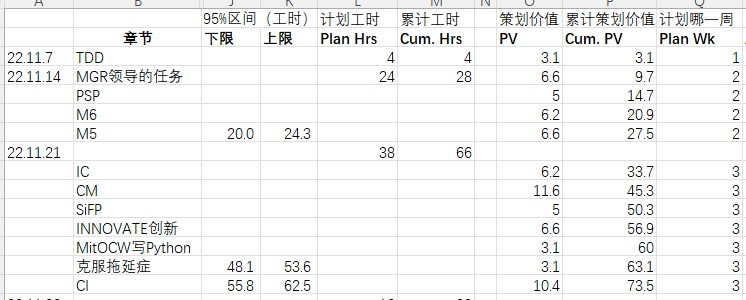
\includegraphics[width=10cm]{PSP3wksPlanScreenshot20221126085813.jpg}

\hypertarget{ux76d1ux63a7}{%
\subsubsection{监控}\label{ux76d1ux63a7}}

按实际完成的情况就可以填右面EV挣值那栋,挣值的算法很简单,必须整个章节完成才算有挣值,不接受部分完成。比如第一周虽然TDD章节已完成九成,但实际是到第二周头才完成,所以第一周的挣值为0。到了第二周才把本来的第一章节完成,所以里面才放上它的PV(=3.1)。监控的好处,好比要准备半年后跑马拉松,开始长距离慢跑LSD锻炼,再进一步做连续马拉松配速训练,每周三天,每次5到15公里,速度是多少?比如平均每公里6:25分钟,有了数字才知道现状与标准的差距,才有动力对自己说现在离比赛不到12周,必须加强锻炼才能赶上。\\
要让项目有更大的机会按期完成,便需要监控,一直可以预计自己离最后交付差距多少?如果按现在的进展要到哪一周才可以完成,应都可以从数字预计出来。但是我们写书也靠灵感,跟写程序类似,可能顺序不一定按本来的执行,怎么办?\\
其实道理也一样,你可以按新的顺序更新一下本来的计划,也把实际的填上。如果你是用简单的Excel表,这个改变可能只花几分钟,很快就能调整好顺序。(例如,本来
现在看到的第二章节,本来计划放在后面才写,但因刚好预客户接触,有灵感,便放在前面写了。)

%\href{文件:PSPend2ndWkEvScreenshot_2022-11-26_091326.jpg}{600px}


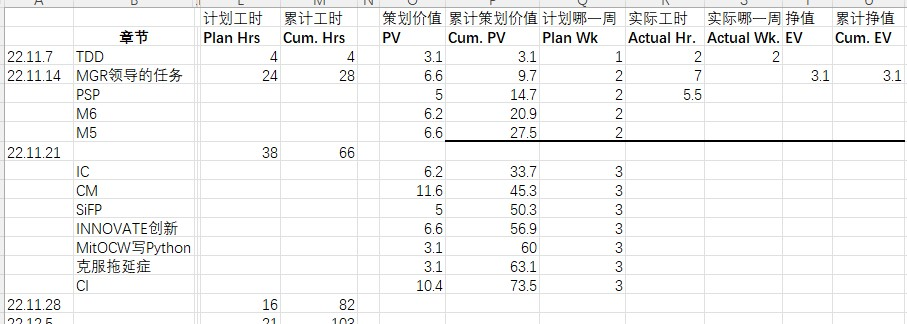
\includegraphics[width=10cm]{PSPend2ndWkEvScreenshot20221126091326.jpg}

要估算任务工时便要依赖以往类似活动的历史记录,如果不是每天记录,过后无法记得住。每周依据个人的习惯,每天记录实际所花小时,然后统计每周累计。但很多人都没有这个习惯,如何养成这个习惯?(详见附件)
\strut
\end{minipage}}

\hypertarget{ux603bux7ed3}{%
\subsection{总结}\label{ux603bux7ed3}}

很多软件开发项目延误(或到交付前团队通宵达旦加班)的原因是因为以前没有收集历史数据,导致估计所需人时都很理想。我也有同样问题:从我的挣值分析实例看到,因我是第一次写书,之前也没有养成统计章节所花的实际工时的习惯,所以在11月初做估算时,理想地认为可以最多花一个月完成,但过了3周就发现,实际比本来计划延误很多,原因包括:

\begin{itemize}
\tightlist
\item
  实际可用工时没有想象这么理想,有很多意外事情都要处理。
\item
  低估了完成一章节所需时间:

  \begin{itemize}
  \tightlist
  \item
    例如第一个章节TDD实际所花的工时与估计差不多,原因是这个章节是现有的,只是做了一些调整,所花时间不多;
  \item
    但到第二个章节MGR就不一样了,全部内容都是重新写的,也是从实际的客户现场、场景总结出来,如何与理论结合也很花心思。
  \end{itemize}
\end{itemize}

所以下次当你遇到一些团队项目延误,可以问组长,或者项目经理,如下问题:

\begin{enumerate}
\tightlist
\item
  如何估算项目工期\\
\item
  如何估算每一项任务所需的工时,依据什么?\\
\item
  如何收集实际工作量\\
\item
  如何监控累计到现在的完成情况\\
\item
  有没有统计以往的历史数据?如何用来帮助做好估算?\\
\end{enumerate}

他可能说都有做,当你深入探索时,会发现很多类似我前面挣值分析、监控和估算等问题。

\hypertarget{ux5e94ux8be5ux5982ux4f55ux6539ux5584}{%
\subsection{应该如何改善}\label{ux5e94ux8be5ux5982ux4f55ux6539ux5584}}

软件开发和工业生产不同,工作量数据必须靠个人自己收集,是一个习惯的问题。所以
Humphrey先生在90年代,推出了PSP个体软件过程,教导开发人员如何一步步自己收集数据、自己估算、自己监控,从最基础的记录花多少工时、发现多少缺陷、完成多少代码开始,逐步改善、提升,最终达到管理质量成本,尽量减少缺陷返工。详见附件PSP简介。

也正因为大部分的团队都没有收集数据的良好习惯,没有的PSP的基础,所以就很难要求他们在冲刺回顾时拿出数据,做根因分析,做下一轮的改善,不能从一个定性的管理升为以数据说话、量化管理的状态。反之,当开发人员养成了这习惯,他们就会更清楚知道自己的速度水平和质量水平,不会出现开头说那种情况,对自己的开发质量水平或生产率一无所知,只说已把上级安排的任务尽力做完。\\
有些企业深知量化管理对企业发展很重要,所以在新员工培训时,不仅仅教他们技术技能,也教他开始自己每天记录工时、缺陷数等习惯。
因为新员工入职后,工作习惯就开始养成,后面要改变他们习惯很难。他甚至会觉得既然周边的人都没有这么做,为什么他要统计数据。

\framebox{%
\begin{minipage}[t]{0.97\columnwidth}\raggedright
\textbf{Q\&A}\\
\textbf{资深敏捷顾问}:我大约接近20年前对这个东西比较熟,PSP里边一个包含两个重点:

\begin{enumerate}
\tightlist
\item
  关于个体的估算的内容,这个我看您的文章里边表达的比较充分,
\item
  关于缺陷记录分类统计和根因分析的内容,这一块实际上相当于是cmmi5级里边需要个体配合的地方。我看您几乎没有提到。
\end{enumerate}

我:非常赞同,若要做到本手册后面里提到基于缺陷数据的量化根因分析并改进就要依赖个人记录缺陷与返工工作量,碍于篇幅有限,这里先用人时的估算与监控带出PSP的思路。\\
顾问:我自己也是在某军工航空项目里边用过一次。我们当年计划少跟踪多,大家本来就缺少生产率的概念,所以其实也不知道每天能干什么事,但只要记下来每天干了什么事,然后再往后比照的这个基数做就可以了。无论突然更快了或者更慢了,都需要看看(回顾)到底是为什么。\\
我:您觉得这种方法有用吗?\\
顾问:因为开发是需要创造力的,写新程序其实很难准确估计所需时间,但我后来发现如果估算是由组长负责去做,就能起很大的作用。例如有一次,我看有一个程序员花了一个月时间用java写了某模块,接近一万行代码。虽然我不熟悉Java语言,但觉得代码有点问题。后面我就找另外一个比较资深的组长,三位一起看代码。评审并删除无用的代码,最后剩下不到一百行代码就可以实现了。如果当初我们先做好这模块的估计,就可以避免一个月人时的浪费。所以我建议还是需要估算,但是应该有有经验的技术组长负责。\\
我:很好,你很熟悉敏捷,例如Scrum里用扑克牌方法估算,你觉得怎么样?\\
顾问:我先跟你讲个故事:我参加某冲刺估算会议,它们用扑克牌方法都某功能估算:``数据显示``,其中一位估计是8,另外一位估计是40。为什么会差这么多呢?第一位解释只需要展示数据,确实该工作量不大。但第二位理解就不一样了,包括整个数据的分析、输入和展示等,整个过程工作量确实很大。从这里可以看出,如果没有统一理解需求,就难以估算。所以那次以后,所以需求分析应分成``实体''和``行为'',清晰地写出功能需求,减少误会。\\
我:赞同。Humphrey先生在PSP书里强调,要参考历史数据来做好估算,其实也可适用于敏捷估算。不应但靠人的主观判断。\\
顾问:是的,所以我前面强调必须要有经验的主管去负责估算。估算很重要,但是要程序员自己去估很难。所以PSP二十年前的思路,还能适用于现在的敏捷开发团队,帮助他们做好估算。\\
PSP里强调要评审设计、代码并分析缺陷,当时因为只靠人手,所以会很耗时。现在,我们有类似SONAR的静态扫描工具,就可以像机器人一样,做本来耗时的代码评审工作。但SONAR只能针对一些基本语句问题,针对整个OO设计,我们会建议用我们的CCI工具去扫描(例如,查看有没有类过大等问题),补充SONAR扫描的不足。跟PSP代码评审的思路一样,所有扫描出的问题都必须修正。有些团队觉得问题太多了,只处理掉那些重大的问题,剩下一些可能不会直接影响到功能的问题暂时不处理。我不赞同这思路,这么多的问题其实都是累积出来的,如果从一开始都一直有定期处理清空,就不应该累积大量问题,而且这些问题遗漏下来还是对程序有隐患。\\
我:很赞同,
归根到底还是开发人员缺乏保证质量的意识。最近有个团队也是用工具扫描代码,然后我问他为什么找出的部分问题不处理。他说例如定义某个变量,但是没有用,虽然被扫出是问题,觉得不影响程序的运行就不处理。我解释说,这样就好像放了一个地雷,后面还是会爆炸的,所以还是应该要处理。\strut
\end{minipage}}

PSP
要求评审代码,分析每个发现的缺陷,讨论原因,然后后面改进。所以有些人认为PSP成本太高,只适用于高价值高质量要求的项目里(或作为个人修炼,短暂的时期内使用)\\
有很多自动化开发工具,可以利用它们更好实现PSP的原理,尽量不花太多人的时间,同样可以达到提高软件质量目的。\\
估算很重要,要做好,不仅仅要参考历史数据, 也需要对需求有共同的理解。\\
功能点方法是估算功能需求规模的一种标准,下篇会用些实例介绍如何做功能点估算。

\hypertarget{ux9644ux4ef6}{%
\section{附件}\label{ux9644ux4ef6}}

\hypertarget{ux6323ux503cux5206ux6790ux6cd5earned-value}{%
\subsection{挣值分析法(Earned
Value)}\label{ux6323ux503cux5206ux6790ux6cd5earned-value}}

挣值分析法(Earned
Value),用最简单的例子,来说明挣值分析中PV、EV、与AC的意义。

\begin{description}
\tightlist
\item[]
PV:计划完成多少

AC:完成工作的实际成本是多少?

EV:实际完成了多少工作?
\end{description}

公式:

\begin{description}
\tightlist
\item[]
进度偏差 SV = EV - PV , SPI = EV / PV 完成占计划完成的\%

成本偏差 CV = EV - AC , CPI = EV / AC 完成的价值占实际已花成本的\%
\end{description}

本文实例主要关心进度偏差,所以没有计算 AC

例如:截止到22.11.20 , PV 累加本应是 27.5,EV 只有 3.1

\begin{description}
\tightlist
\item[]
所以 进度偏差 SV = EV - PV = 3.1 - 27.5 = -24.4 工时
\end{description}

用PERT公式估算头三周任务累积工时的95\%区间(工时):\\
不用MonteCarlo模拟,直接把12(=1+4+7)章节任务 的ExpectedValue 加起来\\
计算12步总方差:(方差 = \(Sigma^2\))\\
:总方差 = 每步方差的总和\\
总Sigma(=1.69) \(\sigma\)= 总方差的平方(Sq.Root)

\begin{description}
\item[]
\begin{description}
\tightlist
\item[]
EXCEL 公式为:SQRT(SUM(所有方差范围)) = SQRT(SUM(H3:H15))\\
\end{description}
\end{description}

\begin{description}
\tightlist
\item[]
95\%范围下限(=55.8)

\begin{description}
\tightlist
\item[]
EXCEL 公式为:SUM(所有Expected范围)-2*总Sigma = SUM(F3:F15)-2*I15
\end{description}

95\%范围上限(=62.5)

\begin{description}
\tightlist
\item[]
EXCEL 公式为: SUM(所有Expected范围)+2*总Sigma = SUM(F3:F15)+2*I15
\end{description}
\end{description}

%\href{文件:PSPcalculate3wks95rangeScreenshot_2022-11-26_105325.jpg}{500px}

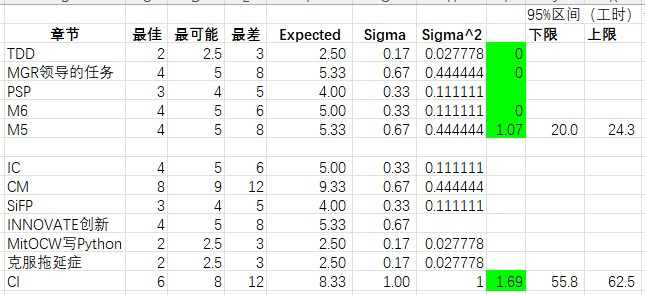
\includegraphics[width=10cm]{PSPcalculate3wks95rangeScreenshot20221126105325.jpg}

\hypertarget{tipsux5982ux4f55ux7b80ux5355ux8bb0ux5f55ux5de5ux65f6}{%
\subsection{Tips:如何简单记录工时}\label{tipsux5982ux4f55ux7b80ux5355ux8bb0ux5f55ux5de5ux65f6}}

如前面``克服拖延症''里提到,每人根据自己的习惯,采用每日ToDoList的方式,然后在开始前,简单记一下时间,结束时也记下时间。然后每日/每周统计每任务总工时:

%\href{文件:Psp手工时间表1.2.jpg}{550px}

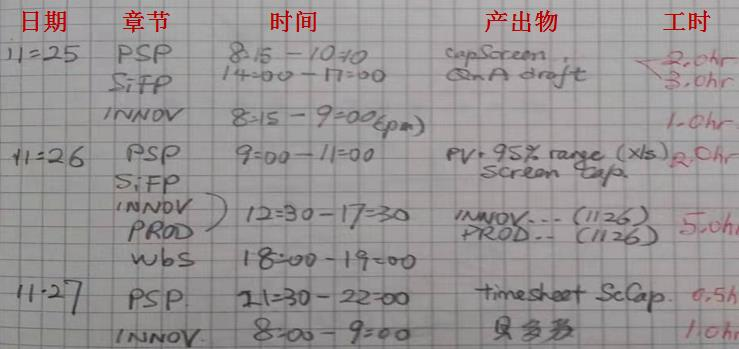
\includegraphics[width=10cm]{Psp手工时间表12.jpg}

(如只是个人,不一定需要项目管理工具;如果是团队,可把自己手工记录上传到项目管理工具,方便团队记录与监控。)

\hypertarget{psp---ux4e2aux4f53ux8f6fux4ef6ux8fc7ux7a0b-personal-software-process-ux7b80ux4ecb}{%
\subsection{PSP - 个体软件过程 Personal Software Process
简介}\label{psp---ux4e2aux4f53ux8f6fux4ef6ux8fc7ux7a0b-personal-software-process-ux7b80ux4ecb}}

\framebox{%
\begin{minipage}[t]{0.97\columnwidth}\raggedright
PSP 的简单介绍\\

\begin{itemize}
\tightlist
\item
  \textbf{PSP0} 基础 - 工时:计划与实际对比; 每阶段引入多少缺陷 ;
  排除了多少缺陷
\item
  \textbf{PSP0.1} 加入 代码行统计 - 计划与实际对比 ; 代码规范
\item
  \textbf{PSP1} 加入 使用 PROBE 方法 做规模估算
\item
  \textbf{PSP2} 加入 设计 与 代码评审的计划与统计
\item
  \textbf{PSP3} Cyclic process - 先做策划与总体设计,然后多轮开发 ;
  有点类似迭代开发。
\end{itemize}\strut
\end{minipage}}

PSP跟CMMI成熟度模型类似,也是按部就班一步步,帮助软件工程师利用度量改进自我的开发过程。

\hypertarget{psp-0.1}{%
\subsubsection{PSP 0.1}\label{psp-0.1}}

第一步PSP先估计写某个模块所需要的时间和实际花的时间,记录所有的缺陷,包括因为需求、设计或者实现引起的问题,记录修复时间,从开始发现问题直到缺陷被解决,提升到PSP0.1策划不仅仅是估计所需时间,加入了规模的概念,本来PSP是用代码行数来估计规模,也可以使用简化功能点方式估计规模大小。\\
在PSP0.1的阶段还没有用规模做策划、估算,只是记录实际的规模,里面包括基本规模,就是在开发之前软件系统本来有多大。也记录删除、改变、增加、复用的规模数等等。最后总的规模数应该是等于基本、新增、删除、复用相加。

\hypertarget{psp1}{%
\subsubsection{PSP1}\label{psp1}}

下一步,PSP1就有规模计划的概念,跟依据0.1的规模定义一样,我们在做开发之前,先估计刚才的所有规模数,并用回归方程估算对应的工作量或者进度,包括偏差的范围。\\
在
PSP0.1增加了一个过程改进建议的环节,依据上一次迭代的数据,发掘下一轮可以完善的改进过程。也加入了编码标准,这个跟我们前面章节提到代码规范的概念相同。所以在PSP0.1,除了计划,也需要有一个叫过程改进经验教训的部分,每一轮都应该有复盘回顾的概念,来提升个人个人的开发过程。

\hypertarget{psp1.1}{%
\subsubsection{PSP1.1}\label{psp1.1}}

PSP1.1基于的PSP1的基础,加入挣值分析法去监控实际的项目进展,加入了PV和累加的PV,计划多少和EV挣值和累计的挣值,反应实际完成多少。从那些系数也可以算出一个叫CPI成本性能指数,来反应完成与计划怎么比较,是否有延误,预计什么时候可以完成。详细可以看用挣值分析法估计写书完成时间的实例。

\hypertarget{psp2}{%
\subsubsection{PSP2}\label{psp2}}

到PSP2就开始增加评审的概念,包括设计评审、代码评审。这些同行评审是很有效的方式,避免缺陷等到出事才暴露、出现问题,因为如果只依赖测试暴露缺陷的话,只是告诉你这个程序跑不通,你还是要看代码才知道问题在哪里,怎么修正?但评审就直接看代码,首先它可以让很多缺陷在评审就发现,就不要等到测试才暴露问题。评审也可以找出一些不一定测得出来的问题,例如有些银行的系统质量要求很高,核心的算法不能有任何错误,他们都会要求核心模块必须走专家评审,因为他们也知道很多一些核心算法的问题不能单靠测试来发现和处理。
也是这个原因,很多公司也会要求代码必须走静态扫描,利用扫描机器人评审代码,预先发现一些明显代码违规的语句问题,弥补单靠人手去评审衡的不足。\\
有了2的基础,2也开始加入缺陷密度的概念,即缺陷数除以模块的规模大小,本来PSP是使用代码行的,我们也可以用功能点取代代码行,因为单看缺陷数无法比较,无论个人自己或者整个团队或者团队之间,所以必须除以规模大小,才可以把系数归一,变成一个项目组之间,人之间可以比较的系数。也引入了排除率的概念,如果我们只是做了评审,但是都是0发现,你的缺陷排除率就是零了,一点效果都没有,所以排除率可以看成是当前评审发现的缺陷数除以当前系统内总共引入的缺陷数,比率越高越好。也有阶段或者过程的排除率,就是这个阶段开始时总共有多少缺陷,然后在这个阶段里我们找出多少,作为分子的一个比例。还有一个就是缺陷排除的速度,按每小时评审的时间找出多少缺陷来判断评审中,可以找出缺陷的速度有多快,评审的效率有多高。

评审质量是PSP2.1 的概念,2.1
也增加质量成本(COQ)概念,与前面敏捷回顾篇里强调软件开发缺陷越后发现,返工量会几何式上升的思路一致。

\hypertarget{psp3}{%
\subsubsection{PSP3}\label{psp3}}

接近敏捷迭代的思路,把程序分成不超于几百行的模块,然后把模块按优先级分到不同的迭代
,但还需要有需求与设计。敏捷增加了精益的思路,因为需求可能会有变,所以可以暂时不做后面迭代的估算,只先针对当前的迭代去做策划、估算。
敏捷里面的迭代回顾跟PSP的回顾如出一辙。\\
大家可以参考PSP书里面的教材和练习,比如在书中要求学员自己编写程序,自己记录时间。虽然现在开发语言统计方法跟90年代有差异,但原理还是共通的。如果对新员工难以安排学校式的一周课程,也可以考虑用自学的形式,按要求去记录学习、写报告。

\framebox{%
\begin{minipage}[t]{0.97\columnwidth}\raggedright
学PSP,培养好习惯
所以编程人员可以用PSP的原则,要他们记录。因为现在是写程序,不是玩游戏,所以更贴近实际。也要求后面的程序,让他分析自己的返工、质量成本、缺陷排除等,让后面项目团队回顾时有真实数据做分析。

例如在新员工培训时,
在练习中,要求他们有编码规范的概念,按照公司的规范参考来写程序,在每一次做开发之前,都先简单计划一下时间和预估缺陷数。开发完后,记录实际的时间与缺陷数,因为虽然不仅仅是写一个程序,是一个系列,在做下一次开发时,可以参考以往练习的数据来更好估计,会看到自己的估计越来越准。\strut
\end{minipage}}

\hypertarget{references}{%
\section{References}\label{references}}

1. Humphrey, Watts S.: "A Discipline for Software Engineering"\\
2. Humphrey, Watts S.: "PSP: A Self-Improvement Process for Software
Engineers" (2005)\\


%done-1
%\chapter{估算软件规模} % Introduction chapter suppressed from the table of contents


\hypertarget{ux4e3aux4ec0ux4e48ux8981ux4f30ux89c4ux6a21}{%
\subsection{为什么要估规模}\label{ux4e3aux4ec0ux4e48ux8981ux4f30ux89c4ux6a21}}

规模可以帮我们:

\begin{enumerate}
\tightlist
\item
  依据历史数据策划,例如估算工作量、工期
\item
  归一(Normalize)不同项目,作比较
\item
  知道现在水平
\end{enumerate}

依据历史数据策划 先把项目分成组件,参考以往类似的组件所花工作量,估算整个项目的总工作量。规模大小可简单看成是组件的数量。 (如果是新开发,以前从未做过同类开发,就只能靠个人经验直接估算工作量(或工期), 但是如果以前做过类似的工作,就可以参考以前的历史数据估算。) 
规模可以帮我们把不同项目归一。例如,验收测试缺陷数无法比较,但缺陷率 (
=缺陷数 / 规模) 便可以比较; 生产率(= 规模 / 所花总工时) 便可比。

有了归一后可比较的系数,个人/团队便更清楚当前的水平(质量/生产率),是否在上升或下降。

\hypertarget{ux4e3aux4ec0ux4e48ux4e0dux5e94ux7528ux4ee3ux7801ux884cux6570loc}{%
\subsection{为什么不应用代码行数(LOC)}\label{ux4e3aux4ec0ux4e48ux4e0dux5e94ux7528ux4ee3ux7801ux884cux6570loc}}

在1996年前, IBM 一直使用代码行数估算规模。
之前一直都使用近似机器语言的Assembly Lang.,
但为了提升效率,引入了高层语言 PL/S,发现 不能再用代码行数来估算规模
因PL/S 只需要更少代码行数 也能完成同样功能:

%Screenshotfrom20221220202712.png

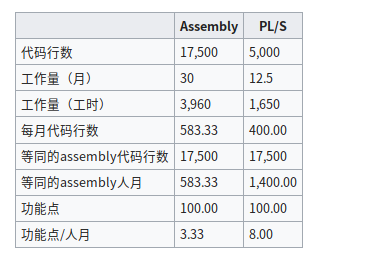
\includegraphics[width=10cm]{Screenshotfrom20221220202712.png}

上表是IBM(1968 - 1975)对两种编译器的统计:\\
每个月 PL/S产出代码行数(400) 反比 Assembly(583) 少

但是如果用功能点数便能真正反映生产率的提升: PL/S : 8.00 对比 Assembly
:3.33

\hypertarget{ux53eaux9002ux7528ux4e8eux7f16ux7801}{%
\subsubsection{只适用于编码}\label{ux53eaux9002ux7528ux4e8eux7f16ux7801}}

看下表,代码行数只能反应编程的工作量,但编码仅占项目总工作量的一部分
如果把项目按工作量分成以下五个部分 代码行数只能用于第二部分编码 (25\%)
其他4部分(30\% + 20\% + 15\% + 10\%)都不合适。

%Screenshotfrom20221220202832.png

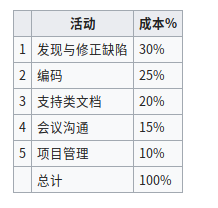
\includegraphics[width=10cm]{Screenshotfrom20221220202832.png}

\hypertarget{ux4e0eux529fux80fdux70b9ux6bd4ux8f83}{%
\subsubsection{与功能点比较}\label{ux4e0eux529fux80fdux70b9ux6bd4ux8f83}}

能估算好项目规模应可帮助我们更好估算工作量,规模应具备以下条件:

\begin{enumerate}
\tightlist
\item
  要和工作量有密切相关 - 应该与工作量强相关
\item
  要容易数得出来
\item
  容易在项目早期可以估算到
\end{enumerate}

功能点比较符合以上条件;只要功能需求明确,就可以估算出对应的功能点数。

只要需求明确便可以准确客观的估算功能点数。
因功能点估算已经是国际标准,基于功能点的度量数据可以与其他国家的标杆对比。

\hypertarget{ux600eux6837ux4f30sifp}{%
\subsection{怎样估SiFP}\label{ux600eux6837ux4f30sifp}}

有了功能性需求,并识别出系统范围,就可以开始估算功能点。:

\begin{enumerate}
\tightlist
\item
  数据功能(简称`实体')的数量 * 7 (实体是系统要管理的数据,)
\item
  业务功能(简称`行为')的数量 * 4.6 (行为可以简单看成是增删改查等功能)
\end{enumerate}

\begin{description}
\tightlist
\item[]
简化功能点数 = 上面 1 和 2 的总数
\end{description}

例如,附件例子一:潜水学校新开发项目:

\begin{itemize}
\tightlist
\item
  识别出3个实体和24个行为,得出简化功能点数131.4 = 3 * 7 + 24 * 4.6
\end{itemize}

潜水学校二次开发项目:
有些功能删除,有些功能变更,就需要分开计算动态功能点和静态功能点:

\begin{itemize}
\tightlist
\item
  静态功能点可以看成是整个系统的功能点数,所以变更的功能点数不会引起影响,但删除的话就需要减去。
\item
  动态功能点主要是用于估算本期开发项目的工作量,因为无论变更功能或者删除功能,都会导致有开发工作量,所以不能是零或负数。国际功能点的规定很简单,都加起来。
\end{itemize}

所以这次二次开发的动态功能点是:

\begin{description}
\item[]
\begin{description}
\tightlist
\item[]
2 * 7 + 11 * 4.6 (增加 两个实体和十一个行为)
\end{description}

+ 1 * 7 + 3 * 4.6 (变更 一个实体和三个行为)

+ 0 * 7 + 2 * 4.6 (删除 两个行为)

= 64.6 + 20.8 + 9.2
\end{description}

再加上 4.6 (因为有数据转换,所以需要加一个CFP,等于4.6)\\
最终动态功能点是99.2 (= 64.6 + 20.8 + 9.2 + 4.6)

静态功能点: 新开发 , 加上新增, 减去删除的功能点

\begin{description}
\item[]
\begin{description}
\tightlist
\item[]
= 131.4 + 64.6 - 9.2

= 186.6
\end{description}
\end{description}

\hypertarget{ux4eceux6545ux4e8bux70b9ux8f6cux7b80ux5316ux529fux80fdux70b9}{%
\subsection{从故事点转简化功能点}\label{ux4eceux6545ux4e8bux70b9ux8f6cux7b80ux5316ux529fux80fdux70b9}}

因故事点只是每个团队自己定义,无法用来作为组织级标准衡量规模,所以很多公司(尤其是银行)转用功能点来衡量软件开发规模。它不仅可用于公司内,也适用于行业标杆,功能点也适用于公司内或公司间结算,例如软件维护期里开发工作量变化很大,也难以事前预估,所以有些银行会按最终开发出来的功能点数结算使用部门付开发部的费用,减少争议。

虽然功能点分析源自70年代,但由于计算较复杂,一直未普及,有些人觉得IFPUG
FPA太复杂。针对这问题,国际功能点协会简化本来的功能点算法,推出简化功能点(SiFP),减少了估算的工作量与学习难度(例如,培训可以从以往的2天半降到半天)。因简化功能点不考虑实体/行为的复杂度,它与本来功能点的估算有\(\pm\)
15 \textasciitilde{} 20\% 偏差(详见附件例子)。
因敏捷团队是按每轮迭代估算(而不是一次性估整个项目),偏差就可以接受
(例如,2周一个迭代,偏差大概1.5天),所以SiFP
能适用于敏捷多次迭代估算。所以越来越多团队开始从故事点转简化功能点,但由于不熟识功能点估算是从用户角度估算,而非从开发工程师的视角看,团队初次估算SiFP通常有误。下面是某成都团队从故事点转简化功能点的案例:

\framebox{%
\begin{minipage}[t]{0.97\columnwidth}\raggedright
客户:我们以前一直使用故事点,为了更好做量化管理,我们新的项目开始使用简化功能点
- SiFP\\
我:好的,看一下你的估算表 。 。 。 。
为什么这两个功能要分成两个行为?\\
客户:这两个功能都挺复杂,估计需要很多开发工作量;我们以前用故事点估算时,也会分成两个故事点。\\
我:请注意,在功能点估算, 是否是一个行为,取决于它算不算是一个基本过程
如果俩行为互相依赖,不能单独作为基本过程,就不应该分开为2个功能点。很多团队刚开始用功能点,与你们一样,没有弄清楚基本过程的概念,还是从工程师的角度,估计开发时间的工作量来判断是一个功能还是两个功能?在故事点用这种方式估算习惯,但因为功能点是要同一个功能上需求,不能有功能点数的差异,所以不能用估计开发难易程度来判断。\\
客户:可否举个实例?\\
我:以网约车为例,是否可以分成以下9个''行为``?

%\href{文件:sifp_p50图.jpg}{600px}

\includegraphics[width=10cm]{sifpp50图.jpg}

\begin{enumerate}
\tightlist
\item
  预约申请
\item
  接收预约
\item
  检查是否有可用的车/司机
\item
  寻找其他可选
\item
  提供预约信息
\item
  处理预约
\item
  分派司机
\item
  接乘客
\item
  完成预约请求
\end{enumerate}

客户:是的,每个行为都要花一定开发工作量。\\
我:其实按SiFP只有4个行为,因头5个,和最后2个都要合并才可以成行为(详见附件)。
如果要能独立成行为,必须符合基本过程条件。
基本过程不是随便定的,它有规则,比如从网约车案例我们可以看到,``预约申请''本身不能算一个基本过程,虽然预约申请可能要很复杂的开发工作,但是因为它不能独立存在,必须依赖其它的行为才算完整。\\
例如,某公司财务系统有打印支票功能(用来付供应商),你觉得打印支票本身是否算基本过程?\\
客户:听完你网约车例子,应该不算;因打印支票只是付款流程的一个可选部分。\\
我:正确、算实体也应使用同样概念。例如,某人事管理系统,除了管理职工信息外,还有员工家属信息,因家属信息必须关连到员工信息,不能独立存在,所以家属信息本身不算是一个实体。你是否觉得你这表里的某些实体应合并?\\
客户:听完你的解释,同意我们这次计算有些实体应合并。\\
我:你们的功能点估算表没有明确区分新的迭代怎么处理变更与删除。
也没有明确动态功能点与静态功能点。\\
客户:我们表中有计算每次迭代的总功能点数。\\
我:你们可能有算每迭代的功能点,但难以看清后面迭代对应之前的变化。动态功能点是用来估算本本迭代的工作量,而静态功能点就是迭代后产品的功能点数。而且应该用表格形式把变更和删除累加在原本上一轮的功能上面,才可以更好看到迭代与迭代之间,功能上的变化。\\
所以不要误以为可以像之前故事点估算,按个人理解写上各种不同复杂程度的故事点例子便可。国际功能点手册里包含很多计算实例,来解释功能点计算,才能确保对同一套需求,每个人,依据用户需求,都能估算出同样的功能点数。我刚刚的例子全都可以从国际功能点手册里找到,你们不需要再发明车轮(reinvent
the wheel)。学功能点估算与写程序类似,必须多动手试。

建议你们读完网约车识别基本过程例子后,再读潜水学校两实例:

\begin{enumerate}
\tightlist
\item
  首次开发
\item
  增强功能与维护 (Enhancement)
\end{enumerate}

觉得已经把握好功能点计算原理,可尝试练习3+4,同样是首次开发+
增强功能与维护。\strut
\end{minipage}}

\hypertarget{ux603bux7ed3}{%
\subsubsection{总结}\label{ux603bux7ed3}}

虽然简化功能点(SiFP)比传统国际功能点IFPUG简单,容易学,但开发人员容易还是用工程师的视角来估算(本应用用户的视角),导致计算错误。所以要多看案例,并做练习才能把握(能参加培训会更好)。

\hypertarget{ux9644ux4ef6}{%
\section{附件}\label{ux9644ux4ef6}}

\hypertarget{ux7b80ux5316ux529fux80fdux70b9sifp-ux7b80ux4ecb}{%
\subsection{简化功能点(SiFP)
简介}\label{ux7b80ux5316ux529fux80fdux70b9sifp-ux7b80ux4ecb}}

 \textbf{它是做什么的?} \\
应用软件开发的客户需求可分成三类:

\begin{enumerate}
\tightlist
\item
  功能性需求
\item
  技术需求
\item
  质量需求
\end{enumerate}

第二类和第三类归为非功能性需求。功能点主要是针对功能性需求,目的是提供对客户有意义的功能点数,来客观地衡量软件规模。

 \textbf{该如何去做?} \\
简化功能点(SiFP)主要两类度量:

\begin{enumerate}
\tightlist
\item
  数据功能 - 实体 (逻辑文件 Logical File)
\item
  事务功能 - 行为(基本过程 Elementary Process)
\end{enumerate}

%\href{文件:功能点计数过程.jpg}{500px}

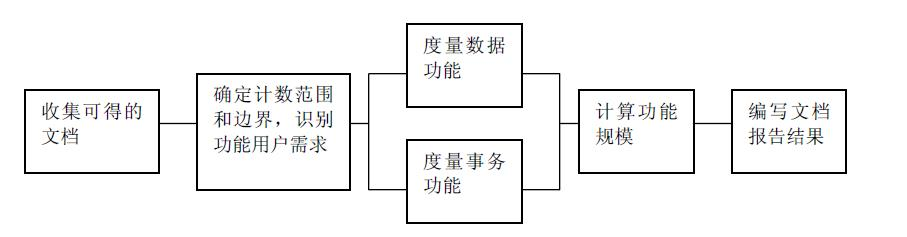
\includegraphics[width=10cm]{功能点计数过程.jpg}

\hypertarget{ux7b80ux5316ux529fux80fdux70b9ux4f30ux7b97ux6b65ux9aa4}{%
\subsubsection{简化功能点估算步骤:}\label{ux7b80ux5316ux529fux80fdux70b9ux4f30ux7b97ux6b65ux9aa4}}

\begin{enumerate}
\tightlist
\item
  确定功能点分析类型
\item
  识别分析范围和应用边界
\item
  计算数据类型功能点(Data Function)
\item
  计算交易类型功能点(Transaction Function)
\item
  计算功能点
\end{enumerate}

\hypertarget{ux4e09ux79cdsifpux8ba1ux7b97ux7c7bux578b}{%
\subsubsection{1:三种SiFP计算类型}\label{ux4e09ux79cdsifpux8ba1ux7b97ux7c7bux578b}}

\begin{itemize}
\tightlist
\item
  开发(Development )
\end{itemize}

\begin{description}
\item[]
\begin{description}
\tightlist
\item[]
DSFP = ADD + CFP
\end{description}
\end{description}

\begin{itemize}
\tightlist
\item
  应用 (Application or Baseline after the initial development)
\end{itemize}

\begin{description}
\item[]
\begin{description}
\tightlist
\item[]
ASFP = ADD
\end{description}
\end{description}

\begin{itemize}
\tightlist
\item
  更新/增强功能与维护 (Enhancement)
\end{itemize}

\begin{description}
\item[]
\begin{description}
\tightlist
\item[]
ESFP = ADD + CHG + DEL + CFP
\end{description}
\end{description}

%Screenshotfrom20221220202712.png

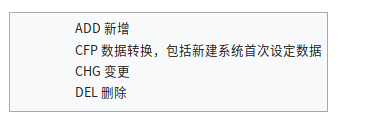
\includegraphics[width=10cm]{Screenshotfrom2022122020-31-37.png}

\hypertarget{ux8bc6ux522bux5206ux6790ux8303ux56f4ux548cux5e94ux7528ux8fb9ux754c}{%
\subsubsection{2:识别分析范围和应用边界}\label{ux8bc6ux522bux5206ux6790ux8303ux56f4ux548cux5e94ux7528ux8fb9ux754c}}

例子:用虚线标示系统边界:\\
%\href{文件:功能点计数P62_2.0.jpg}{500px}\\

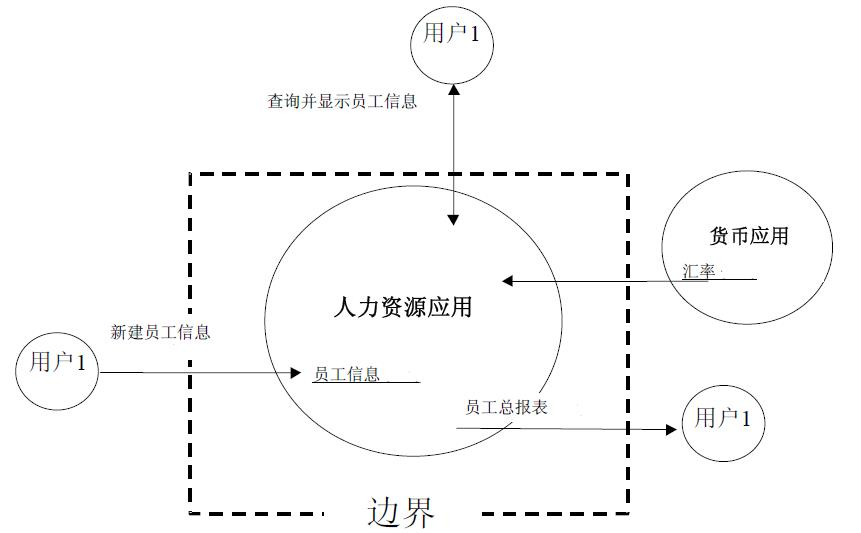
\includegraphics[width=10cm]{功能点计数P6220.jpg}

\hypertarget{ux8ba1ux7b97ux903bux8f91ux6587ux4ef6ux6570}{%
\subsubsection{3:计算逻辑文件数}\label{ux8ba1ux7b97ux903bux8f91ux6587ux4ef6ux6570}}

\begin{itemize}
\tightlist
\item
  关于计算规则,详见"逻辑文件"
\end{itemize}

\hypertarget{ux8ba1ux7b97ux57faux672cux8fc7ux7a0bux6570}{%
\subsubsection{4:计算基本过程数}\label{ux8ba1ux7b97ux57faux672cux8fc7ux7a0bux6570}}

\begin{itemize}
\tightlist
\item
  关于计算规则,详见"基本过程"
\end{itemize}

\hypertarget{ux8ba1ux7b97ux529fux80fdux70b9}{%
\subsubsection{5:计算功能点}\label{ux8ba1ux7b97ux529fux80fdux70b9}}

\begin{itemize}
\tightlist
\item
  每个逻辑文件 = 7.0 简化功能点
\item
  每个基本过程 = 4.6 简化功能点
\end{itemize}

\hypertarget{ux903bux8f91ux6587ux4ef6-logical-file}{%
\subsection{逻辑文件 Logical
File}\label{ux903bux8f91ux6587ux4ef6-logical-file}}

\textbf{(下面在计算实例里简称``实体'',方便理解)}

\begin{itemize}
\tightlist
\item
  用来储存内部或外部数据,是用户可识别的逻辑相关的数据组或控制信息组,在被度量应用边界内部维护。
\end{itemize}

\begin{description}
\tightlist
\item[]
(\textbf{用户可识别} -
用户可识别 -指数据或事务需求是被用户和软件开发人员双方共同认同并理解的。
例如:用户和软件开发人员双方都认同人力资源应用有维护和存储员工信息的功能。)
\end{description}

\hypertarget{ux6ce8ux610f}{%
\paragraph{注意}\label{ux6ce8ux610f}}

逻辑文件包括两类不同的用户需求数据:

\begin{enumerate}
\tightlist
\item
  功能性数据
\item
  非功能性数据
\end{enumerate}

功能性数据是用来满足用户功能需求的数据。例如,销售、银行账号、供应商、人员等信息。\\
非功能数据主要是为了满足易用性(支撑下拉菜单所需的数据,可输入数据的上下范围等);或性能方面(用于查询数据的索引index);或可维护性(配置参数)。\\
只有第一类功能性数据才算是逻辑文件。\\

\hypertarget{ux57faux672cux8fc7ux7a0b-elementary-process}{%
\subsection{基本过程 Elementary
Process}\label{ux57faux672cux8fc7ux7a0b-elementary-process}}

基本过程是对用户有意义的最小活动单元。例如:添加员工的用户需求包括建立工资和家属信息。只有添加所有员工信息,才能创建员工信息记录。单独添加一些信息使添加员工业务处于不持续状态,只有员工工资和家属信息都添加后,这个活动单元才能完成且业务处于稳定状态。

\hypertarget{ux8bc6ux522bux57faux672cux8fc7ux7a0b}{%
\subsubsection{识别基本过程}\label{ux8bc6ux522bux57faux672cux8fc7ux7a0b}}

为了识别基本过程,需要执行以下活动:

\begin{itemize}
\tightlist
\item
  把功能用户需求分解为最小活动单元,使其满足下面条件:

  \begin{itemize}
  \tightlist
  \item
    对用户有意义\\
    例如:功能用户需求要求在应用中添加新员工的能力。\\
  \item
    构成一个完整的事务\\
    例如:用户定义的员工信息包括工资和家属信息。如果家属人数大于零,添加员工信息时必须包括家属信息。本例中,添加员工信息(不包括添加地址、工资和家属信息)不满足本规则。\\
  \item
    自包含\\
    例如:除非输入所有的必需信息并且完成所有处理步骤,如验证、计算、更新ILFs,添加过程才是自包含的。\\
  \item
    让应用程序的业务保持持续状态\\
    例如:添加员工的用户需求包括建立工资和家属信息。只有添加所有员工信息,才能创建员工信息记录。单独添加一些信息使添加员工业务处于不持续状态,只有员工工资和家属信息都添加后,这个活动单元才能完成且业务处于持续状态。\\
  \end{itemize}
\end{itemize}

识别活动单元为基本过程需要满足以上所有规则。\\

\hypertarget{ux8bc6ux522bux57faux672cux8fc7ux7a0bux4e3bux8981ux76eeux7684}{%
\subsubsection{识别基本过程主要目的}\label{ux8bc6ux522bux57faux672cux8fc7ux7a0bux4e3bux8981ux76eeux7684}}

基本过程的主要目的可识别为下列情形的一种:

\begin{itemize}
\tightlist
\item
  改变应用行为
\item
  维护一个或多个ILFs
\item
  呈现信息给用户
\end{itemize}

\hypertarget{ux5b9eux4f8bux8bc6ux522bux57faux672cux8fc7ux7a0b-ep-elementary-process}{%
\subsection{实例:识别基本过程 (EP elementary
process)}\label{ux5b9eux4f8bux8bc6ux522bux57faux672cux8fc7ux7a0b-ep-elementary-process}}

下面是某预约网约车过程:

%Screenshotfrom20221220203338.png

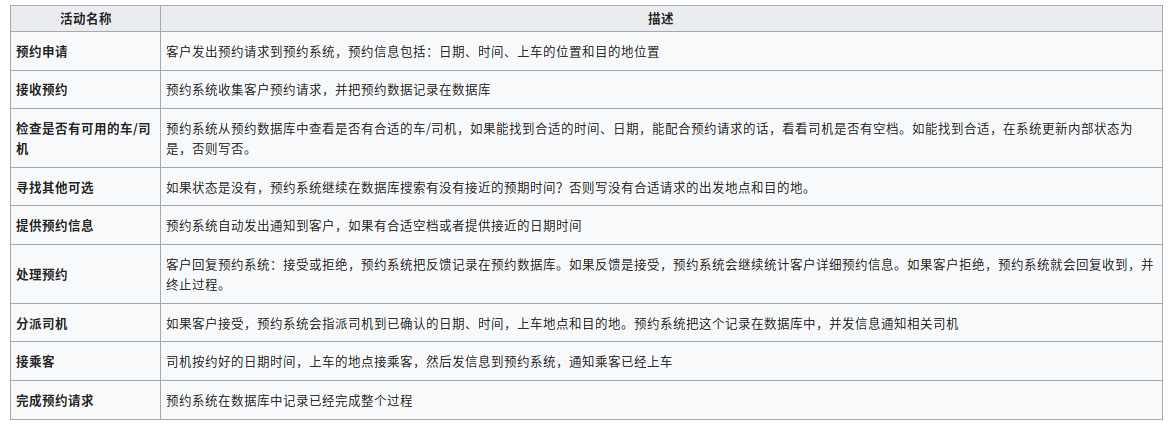
\includegraphics[width=10cm]{Screenshotfrom20221220203338.png}

\textbf{分析能否满足所有 EP 识别规则,判断能否独立成为基本过程 (EP
elementary process),部分例子}

\hypertarget{ux9884ux7ea6ux7533ux8bf7}{%
\subsubsection{预约申请}\label{ux9884ux7ea6ux7533ux8bf7}}

\begin{enumerate}
\tightlist
\item
  是否对用户有意义,客户功能需求的一部分?\textbf{是}
\item
  是否构成一个完整的事务?\textbf{否}:预约申请本身不是一个完整的交易,因为过程必须也包括预约请求信息,收到其它可选的档期这些步骤,都不可以分离。
\item
  是否自包含,可以独立存在?\textbf{否}:例如,接受预约申请;查看是否有档期,查看有没有其它接近的档期等,都是一些必须的相关步骤去完成这个基本过程。
\item
  是否让应用程序达到稳定状态?\textbf{否}:整个业务需求只能在收到预约信息,发送、接受、处理、反馈给客户才算是完成稳定状态。
\end{enumerate}

\hypertarget{ux5206ux6d3eux53f8ux673a}{%
\subsubsection{分派司机}\label{ux5206ux6d3eux53f8ux673a}}

\begin{enumerate}
\tightlist
\item
  是否对用户有意义,客户功能需求的一部分?\textbf{是}
\item
  是否构成一个完整的事务?\textbf{是}:分配到司机是一个完整的交易,包括收到司机的确认,把信息记录在系统中并通知司机。
\item
  是否自包含,可以独立存在?\textbf{是}:分配到司机本身可以独立存在。
\item
  是否让应用程序达到稳定状态?\textbf{是}:因为当司机被分配后,是完全满足业务的需要。
\end{enumerate}

\hypertarget{ux63a5ux4e58ux5ba2}{%
\subsubsection{接乘客}\label{ux63a5ux4e58ux5ba2}}

\begin{enumerate}
\tightlist
\item
  是否是客户功能需求?\textbf{是}
\item
  交易是否完整?\textbf{否}:接乘客本身不算一个完整的交易,因为预约系统必须也记录这个信息。
\item
  是否自包含,可以独立存在?\textbf{否}:确认预约申请是下面一个必须执行的过程,来完成这个基本过程。
\item
  是否让应用程序达到稳定状态?\textbf{否}:整个业务需求只能在和预约系统确认沟通,已经接到乘客,然后系统也把记录更新到预约系统才算完成。
\end{enumerate}

%Screenshotfrom2022122020-34-37.png

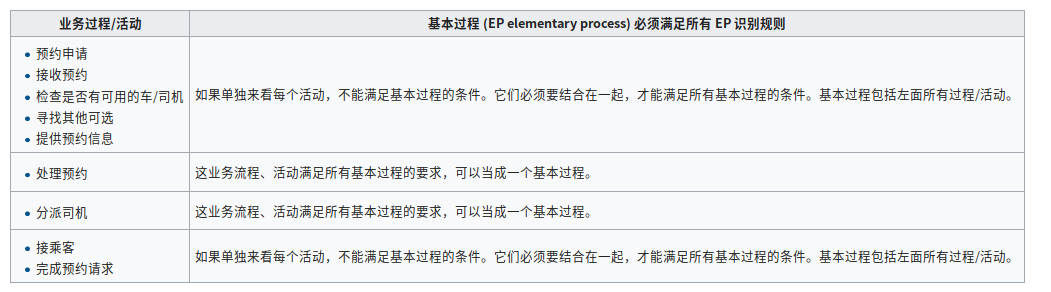
\includegraphics[width=10cm]{Screenshotfrom2022122020-34-37.png}


\hypertarget{ux4e0eux56fdux9645ux529fux80fdux70b9ifpugux7684ux504fux5dee}{%
\subsection{1.潜水学校:开发项目 }\label{ux4e0eux56fdux9645ux529fux80fdux70b9ifpugux7684ux504fux5dee}}

\hypertarget{ux63a5ux4e58ux5ba2}{%
\subsubsection{描述}\label{ux63a5ux4e58ux5ba2}}

一所潜水学校需要一套用来管理合同员工(教练)、设施、轮班工作的系统。目的:有效地管理教练在潜水设施和几艘旅游潜水船上有关潜水课程/短途潜水的轮班工作。 \\
\hypertarget{ux63a5ux4e58ux5ba2}{%
\subsubsection{功能需求}\label{ux63a5ux4e58ux5ba2}}

该系统将包括菜单界面和定期运行的批量处理等功能。\\
The system will consist of an online component based on a menu interface and a batch component that will run periodically. \\

\hypertarget{ux63a5ux4e58ux5ba2}{%
\subsubsection{RF01}\label{ux63a5ux4e58ux5ba2}}

为处理教练保险单文件,并符合法例,学校需要为每个合同员工储存以下资料: \\


\begin{itemize}
\tightlist
\item
  序列号(独特,作为索引, 不能重复)
\item
  姓名
\item
  居住地址
\item
  城镇
\item
  邮政编码
\item
  电话号码
\item
  是否持有航海执照
\end{itemize}

为了跟踪每个合同员工的“职业生涯”,学校决定给予他们以下分类: \\
1.“潜水长”
2.“助理教练”
3.“教练”

这些分类是固定的,并不会随着时间而转变:每个合同员工会按顺序分配到合适的类别,代表个人“职业生涯”的发展(例如,一个新员工开始是“潜水长”,随着时间的推移,他会成为“教练”)。\\

使用表单输入,显示,编辑和删除合同员工的数据。会有一个独立列表框,显示序列号、名和姓 (但没有附件明细),来选择要编辑、删除或详细查看的是哪位员工的数据。\\


用功能键激活所有的功能,并最终产生一个结果或错误信息。“删除合同员工”只是在逻辑上删除,没有数据会被物理删除,但会被标记为作废。只要有与其相关的工作班次,合同员工就不能被删除。 \\

\hypertarget{ux63a5ux4e58ux5ba2}{%
\subsubsection{RF02}\label{ux63a5ux4e58ux5ba2}}

%学校还需要管理设施(“潜水”、“船”或“橡皮艇-RD”),每一个设施都有独特的友好名称(例如:“潜水莫格利亚 diving-moneglia”、“潜水帕拉 diving_palau”、“蓝箭艇 blue-arrow-boat”、“格里大艇 goletta-boat”、“嘉莉花RD Genova_RD”等等)。\\

对于每种类型的设施,必须存储以下信息: \\

\begin{itemize}
\tightlist
\item
  设施识别名(独特,作为索引,不能重复)
\item
  描述
\item
  类型
\item
  它能容纳的人数
\item
  可用汽缸数
\item
  是否有厕所
\item
  是否有饮用水储备
\end{itemize}

必须创建表单来输入、显示、编辑和删除设施数据;如果有被分派到轮班,就不能删除设施。使用独立的列表(不显示附件细节),以便选择要编辑、删除或详细查看的数据,列表只展示:标识名称、描述、类型\\
用功能键来激活某功能,并最终生成错误或结果信息。 \\

\hypertarget{ux63a5ux4e58ux5ba2}{%
\subsubsection{RF03}\label{ux63a5ux4e58ux5ba2}}

最后,为了有效管理分派轮班(shift)的覆盖范围,学校需要处理合同员工以下轮班(shift)信息: \\

\begin{itemize}
\tightlist
\item
  工作轮班识别名(独特,作为索引,不能重复)
\item
  可用的合同员工编号(使用下拉框挑选)
\item
  提供本轮班可用的日期
\item
  可用期的开始日期
\item
  可用期的结束日期
\item
  首选设施(使用下拉框挑选)
\item
  状态(最初预设置为“预计轮班”)
\end{itemize}

必须创建表单来输入、显示、编辑和删除轮班(shift)的有效信息。为了方便选择对哪些数据进行编辑、删除或查看详细信息,会独立显示没有附件细节的数据列表(如,不显示可用性标识号,合同员工序列号)。用功能键将激活这功能,并最终生成错误/或结果信息。 \\

\hypertarget{ux63a5ux4e58ux5ba2}{%
\subsubsection{RF04}\label{ux63a5ux4e58ux5ba2}}

每个合同员工可以提供不止一个可用轮班(availability),每一个轮班最初都设定为“预计轮班tentative shift”状态。\\
当分配协调各合同员工的可用轮班作为一个“轮班(shift)”内的可用资源时,秘书处在一个“分配轮班 assigned shift”内使用特定命令选择(转换)所需的可用轮班(availability),她可以更改潜水期的开始和结束日期,并可以将之设定为“分派轮班”状态。删除“分派轮班”与删除“预计轮班”的功能/步骤类似。 \\


\hypertarget{ux63a5ux4e58ux5ba2}{%
\subsubsection{RF05}\label{ux63a5ux4e58ux5ba2}}

有以下查询:

1.找出合同员工中谁已经有许可证,因此能够以“船夫”的身份带队出海 - 显示属性:序列号。姓和名,和总人数。
2.选择当前某月份(或其他月份和年份)收到的所有可用合同员工——显示的属性:序列号、姓名、类别、可用期的开始日期和结束日期以及对设施的偏好。
3.根据档案中设施的数量和类型,(包括考虑潜水和船数量)计算学校管理的最大人数。
4.计算每个类别的员工人数(潜水主任;助理教练;教练):按类别列出总计和小计。
5.通过显示姓名和姓氏,显示最“忠诚”的员工,即年初以来提供最多可用时间段的前三名员工。
6.上面查询4的增强版: 通过类别细化——换句话说,不仅仅是显示数量,可选择某个类别的相关合同员工列表(姓和名)与其总数量。


\hypertarget{ux4f8bux5b50ux4e00-ux7b54ux6848ux4e0eux89e3ux8bfb}{%
\subsection{例子一:
答案与解读}\label{ux4f8bux5b50ux4e00-ux7b54ux6848ux4e0eux89e3ux8bfb}}

共三个实体:

\begin{enumerate}
\tightlist
\item
  合同员工
\item
  管理设施
\item
  轮班
\end{enumerate}

你可能会问:那些合同员工的职称是否也应该是一个实体?(因需要花工夫开发)\\
这不应该是一个实体,原因:人员的职称必须依赖人员的信息挂在一起,不可以独立存在,就好比我们要维护员工信息,假如也要维护员工的家属信息,这个家属信息就不能算另外一个实体,因为没有人员的话,家属是不能单独存在的。原则:不是根据是否要产生开发的工作量,而是从用户角度看,这个实体能否独立存在和维护。否则功能点的估算就只是根据个人对开发工作量的估计,而不是从用户角度看功能的客观判断。

每个实体对用户来讲,都有新增、展示、修改、删除4个功能。在人员管理里,还有一个功能是显示一个可选的列表,方便用户选择,这功能是增查改删以外的第五个功能。

设施管理也同样有这个列可选设备设施的一个展示框这第五个功能。

在轮班管理里面,除了增加、查看、修改、删除和展示外,它里面有两个下拉框功能:

\begin{enumerate}
\tightlist
\item
  让客户挑选相关设施的 Combo-box下拉框
\item
  让客户选人员的框
\end{enumerate}

你可能会问,这 2
个下拉框功能是否不应该算额外的功能,而是属于``轮班''的增删改查基本功能的一部分?\\
我们可以这样想:从用户的角度来看,如果没有这两个下拉框的功能,基本的增删改查功能是否可以实现;现在做了两个下拉框的功能,是额外的新增功能,更方便用户去选择,所以这两个算是额外两个功能。

也可参考IFPUG关于EI/EO/EQ 的识别要求;基本操作(elementary
process)必须符合以下三条之一:

\begin{enumerate}
\tightlist
\item
  使用独特处理逻辑,与应用中其他`行为'(EI/EO/EQ) 的处理逻辑不同
\item
  在该处理中识别出来的数据元素是与应用中其他`行为'(EI/EO/EQ)
  的数据元素不同
\item
  在该处理中引用的`实体'(ILF 和EIF) 与其他`行为'(EI/EO/EQ)
  所引用的不同
\end{enumerate}

它要列出所有合条件的数据元素进这下拉框,类似一个新的报表,所以算一个行为。基于同类原因,挑选相关设施的
Combo-box 下拉框,选择可用合同员工 Combo-box 下拉框, 等各自也算一个行为。

在轮班里,还有一个展示可选的轮班功能,另外是分配轮班功能。还有最后的
RF05 六个查询功能。

得出共 24(=5+5+6+2+6)行为,加 3实体, 所以按简化功能点每个实体 x7,每行为
x4.6 得出,共新增131.4(=3x7+24x4.6)简化功能点,详见下面列表:

%\href{文件:Ex1SoluScreenshot_2022-04-05_115926.jpg}{500px}

%Ex1SoluScreenshot_2022-04-05_115926.jpg

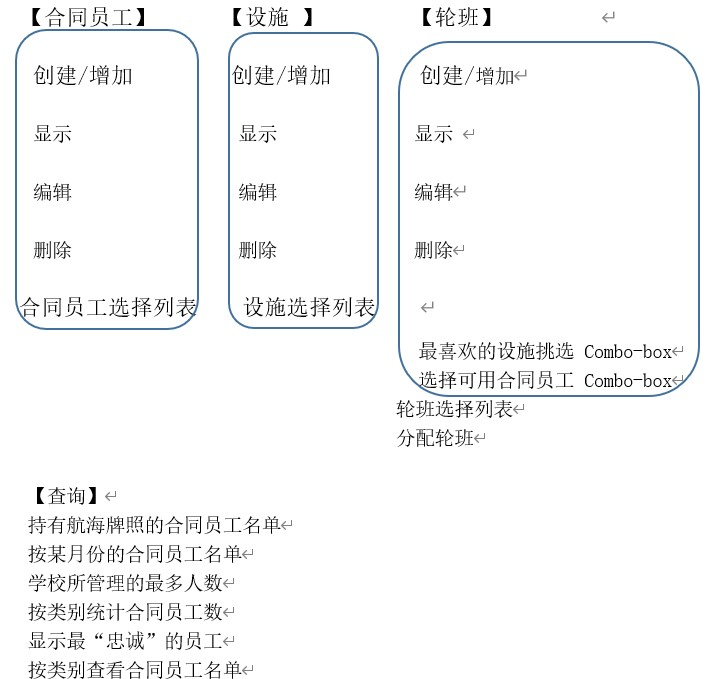
\includegraphics[width=10cm]{Ex1SoluScreenshot_2022-04-05_115926.jpg}

%\href{文件:微信截图_20220412130822.jpg}{550px}

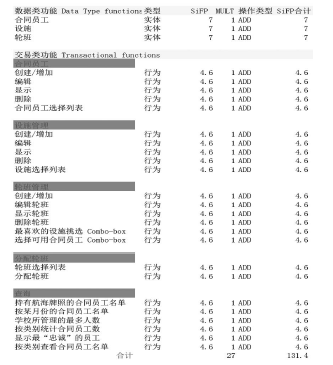
\includegraphics[width=10cm]{微信截图_20230324091110.png}

\hypertarget{ux8ba1ux7b97ux529fux80fdux89c4ux6a21}{%
\subsubsection{计算功能规模}\label{ux8ba1ux7b97ux529fux80fdux89c4ux6a21}}

\begin{description}
\item[]
\begin{description}
\tightlist
\item[]
DSFP = ADD + CFP
\end{description}
\end{description}

因为没有数据转换,所以 CFP=0, 所以 DSFP = (110.4+21) +0 = 131.4 SiFP

因是首次开发, ASFP = ADD = 131.4 SiFP

\hypertarget{ux6f5cux6c34ux5b66ux6821femux9879ux76ee}{%
\subsection{2.潜水学校:FEM项目}\label{ux6f5cux6c34ux5b66ux6821femux9879ux76ee}}

\hypertarget{ux63cfux8ff0}{%
\subsubsection{描述}\label{ux63cfux8ff0}}

参照之前的潜水学校系统,对功能进行了增强,并提出了该软件的功能优化维护项目(FEM)。

\hypertarget{ux529fux80fdux9700ux6c42}{%
\subsubsection{功能需求}\label{ux529fux80fdux9700ux6c42}}

\hypertarget{rf01}{%
\paragraph{RF01}\label{rf01}}

用户想要取消合同员工删除功能。The user wants to eliminate the Contractor
delete function.

\hypertarget{rf02}{%
\paragraph{RF02}\label{rf02}}

在短途潜水里, 在潜水设施管理中能管理船上医生的存在或缺失。The
presence/absence of a ship doctor during excursions must be managed in
the file DIVING FACILITIES.

\hypertarget{rf03}{%
\paragraph{RF03}\label{rf03}}

出于税收和安全原因,不再需要删除可用轮班这项功能 For tax and safety
reasons the function to delete availability shifts will no longer be
required.

\hypertarget{rf04}{%
\paragraph{RF04}\label{rf04}}

用户还需要管理课程参与者信息和他们参加的那个短途潜水信息:\\
*管理参与者的信息包括:参与者ID,姓,名,出生日期,潜水执照,执照日期。\\
参加短途潜水:参与者ID。轮班编号,出游日,天数,最终考试是/否通过\\
*用列表框 (包括:参与者ID,姓,名)来选择轮班中的参与者。\\
*使用原本应用程序中已经有的列表框选择轮班。\\
*用功能键将激活这功能,并最终生成错误信息/结果。

用功能键初始填充课程参与者信息,参与者信息源自以前参与者信息的备份数据。

\hypertarget{rf05}{%
\paragraph{RF05}\label{rf05}}

用户还需要能够在课程结束时颁发出席证书给在短途潜水中登记的所有参与者。除了管理参与者基础数据外,还需要管理:参与者所登记的轮班、轮班日期、时长、教练的姓名和医生(如在场)的姓名。该功能使用原本应用程序中已经可用的功能:选择轮班。用功能键将激活这些功能,并最终生成错误/结果消息。

\hypertarget{rf06}{%
\paragraph{RF06}\label{rf06}}

用户还需要能够向合同员工颁发``教员身份参与证书'',其中的信息除了基础数据外还包括:轮班ID、教练ID、出游日、船医(如果有的话)。对于轮班选择,将使用原本应用程序中已经有的列表框。用功能键将激活这功能,并最终生成错误信息/结果。

\hypertarget{ux4f8bux5b50ux4e8c-ux7b54ux6848ux4e0eux89e3ux8bfb}{%
\subsection{例子二:
答案与解读}\label{ux4f8bux5b50ux4e8c-ux7b54ux6848ux4e0eux89e3ux8bfb}}

RF02 变动了潜水设施的内容,所以设施实体有变更。\\
因为设施的信息有变更,导致跟这实体相关的行为,包括新增、编辑、和展示这三行为都会有变更。

另外加了两个要管理的实体:

\begin{enumerate}
\tightlist
\item
  参与者
\item
  短途潜水
\end{enumerate}

不需要合同员工的删除功能,所以是个行为删除。

在参与者的管理,除了增加,改动,展示和删除四个功能以外,还有可以挑选参与者的下拉框功能。

两个证书的功能

\begin{enumerate}
\tightlist
\item
  给教练的证书
\item
  给参与者发证书
\end{enumerate}

对应每个短途潜水也需要有添加、改动、展示、删除的四功能。
那个删除轮班功能也被删掉了。

增加了两个实体 -\/-参与者 与 短途潜水旅行登记\\
Q: 为什么短途潜水旅行登记算一个实体?\\
A: 因它包括的信息都不能归入已有的 【参与者】 【合同员工】 【设施
】【轮班】实体里,例如那位参与者参加了那个班,考试分数等。
也可参考IFPUG关于ILF/EIF (实体)的识别要求;必须符合以下条件:

\begin{enumerate}
\tightlist
\item
  数据的集合必须是逻辑相关的并且是用户可以识别
\item
  这些数据或者控制信息必须是在本应用的边界内被维护
\end{enumerate}

总结:

\begin{itemize}
\tightlist
\item
  实体方面增加了2 实体; 设施实体有变更。
\item
  行为方面主要的在短途潜水旅行方面增加了4 增删改查的功能和。5
  参与者的功能(因为在里面加了一个下拉框功能),增加了2
  证书功能。改动了设施的增加、编辑、和展示,三个行为,删掉了两个行为。
\end{itemize}

所以动态功能点是增加的功能点64.6 (=2x7 +(4+2+5)x4.6),变更 20.8
(=3x4.6),删除9.2 (=2x4.6),总共的动态简化功能点 94.6。

静态功能点依据上面练习一那的131.4,加上增加的功能点 64.6,减掉
删除功能点 9.2,得出变更后静态功能点 186.8。

%\href{文件:Ex2XlsScreenshot_2022-04-05_143941.jpg}{550px}

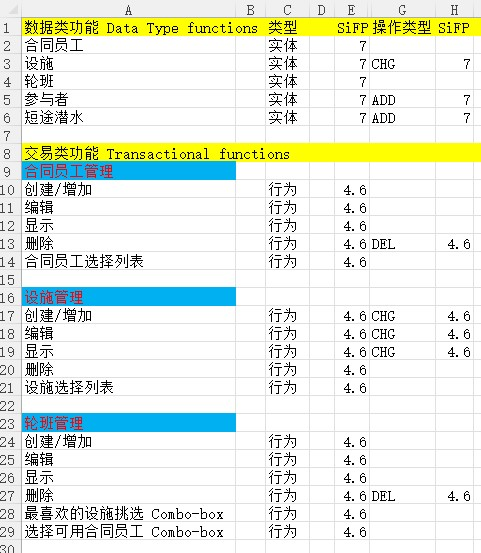
\includegraphics[width=10cm]{Ex2XlsScreenshot_2022-04-05_143941.jpg}

%\href{文件:Ex2XlsPt2of2Screenshot_2022-04-05_143941.jpg}{550px}

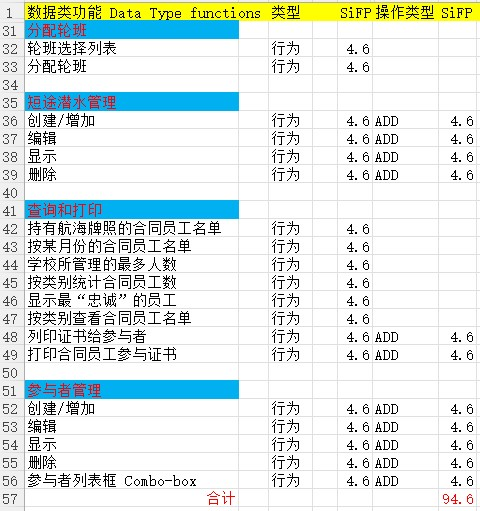
\includegraphics[width=10cm]{Ex2XlsPt2of2Screenshot_2022-04-05_143941.jpg}

\hypertarget{ux8ba1ux7b97ux529fux80fdux89c4ux6a21-1}{%
\subsubsection{计算功能规模}\label{ux8ba1ux7b97ux529fux80fdux89c4ux6a21-1}}

\begin{description}
\item[]
\begin{description}
\tightlist
\item[]
ESFP = ADD + CHG + DEL + CFP
\end{description}
\end{description}

因为有数据转换:初始填充课程参与者信息作为一个基本过程,所以 CFP=4.6

\begin{description}
\tightlist
\item[]
ESFP = (64.6 + 20.8 + 9.2) + 4.6 = 94.6 + 4.6 = 99.2 SiFP
\end{description}

软件开发后的静态功能点: ASFPA = ASFPB + ADD - DEL = 131.4 + 64.6 - 9.2
= 186.8 SiFP


\hypertarget{ux4e0eux56fdux9645ux529fux80fdux70b9ifpugux7684ux504fux5dee}{%
\subsection{与国际功能点(IFPUG)的偏差}\label{ux4e0eux56fdux9645ux529fux80fdux70b9ifpugux7684ux504fux5dee}}

例子:

\begin{itemize}
\tightlist
\item
  新开发某会计付款系统
\item
  实体: 包括管理 发票 ,付款,供货商。
\item
  行为:包括对每个实体的展示,增加,修改,和删除/取消
\item
  使用IFPUG 数 EI, EO, EQ, ILF, EIF
  每类的调整前功能点数,加起来得出调整前功能点数FP=82
  (如想多了解IFPUG如何计算复杂度,参考附件)
\item
  使用SiFP 估算实体和行为数,计算得出 FP=104
\end{itemize}

%\href{文件:FPA_S11.jpg}{500px}

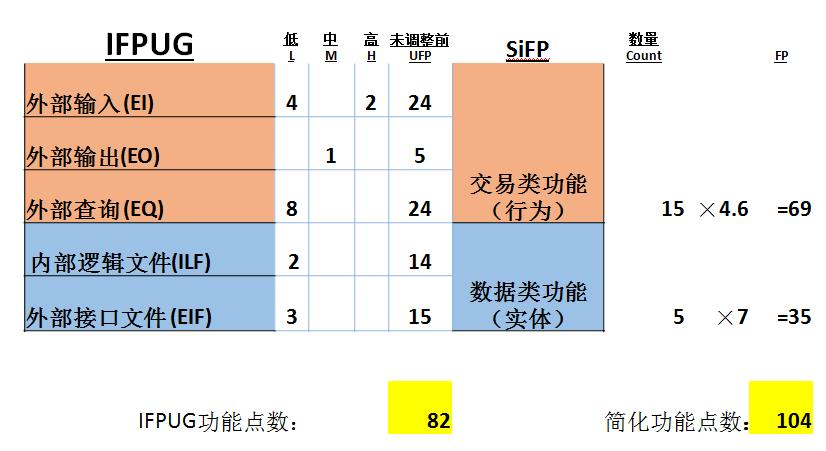
\includegraphics[width=10cm]{FPAS11.jpg}

\begin{itemize}
\tightlist
\item
  IFPUG / SiFP
  得出的实体数量,与行为数量都一样 (实体(=ILF+EIF)=5  行为
  (=EI+EO+EQ)=15)
\item
  因为简化功能点只是不区分实体与行为的复杂度(高中低),取平均值,原理一样,虽然个别估算有差异,但平均下来与IFPUG的估算没有结构性偏差
\end{itemize}


\hypertarget{references}{%
\section{References}\label{references}}

1. BRIGIDO, Sergio: "FPA Rules interpretations for Elementary Processes " , IFPUG Whit paper, 2022
2. SiFPA Assoc.: "Simple Function Point Functional Size Measurement Method, Measurement Examples " , SiFP-0.1.00-EX-EN-01.01 (2014)\\

%done-1
%\chapter{估算工作量} % Introduction chapter suppressed from the table of contents

这几年大数据很火,很多高科技公司都推相关的工具或者方案,很多软件开发项目经理觉得应该也用数据分析,分析历史数据,准确预估项目工作量、工期。

''但实际上,虽然预测模型已经有超过50年的历史,过千份研究报告,教材/指南,但使用在项目中不多。更多研究发现如果用专家估算可能更准确。``\\
以上是 IEEE杂志 2009 的文章中,JORGENSEN先生的结论。在文章里,JORGENSEN
与 BOEHM 两位专家讨论模型与专家估算法的长短:

%\href{文件:估算专家.png}{300px}

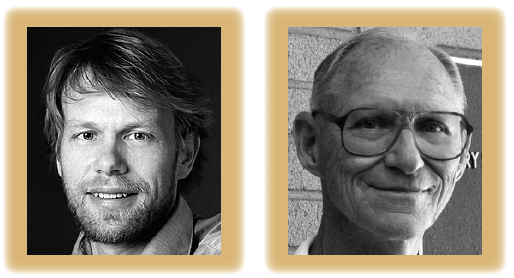
\includegraphics[width=6cm]{估算专家.png}\\

左边:北欧学者 Magne JORGENSEN
过去十多年集中研究软件估算,发现专家估算法虽然很常用,但相关研究却不多\\
右边:Barry BOEHM 81年出版 Software Engineering Economics, 后面又推出
COCOMO 预测模型, 是模型估算的经典人物

\hypertarget{ux4f30ux7b97ux9760ux6a21ux578bux8fd8ux662fux9760ux4e13ux5bb6model-based-vs-expert-based-estimation}{%
\subsection{估算:靠模型,还是靠专家?(Model-based Vs Expert-based
estimation)}\label{ux4f30ux7b97ux9760ux6a21ux578bux8fd8ux662fux9760ux4e13ux5bb6model-based-vs-expert-based-estimation}}

什么是专家估算?最典型的例子,就是WBS估算,我们先把所有的任务,系统地分解出来,召集团队和专家估计工作量(或工期);\\
模型是反过来:利用一些参数模型,如利用功能点数来做其中的一个输入,也包括其他因素,如复杂度、人员能力、平台等。

两种方法的主要区分在于最后估算工作量的步骤:模型(例如COCOMO)通常利用方程式自动从输入估算出结果,如下图:

%\href{文件:估算3.png}{600px}

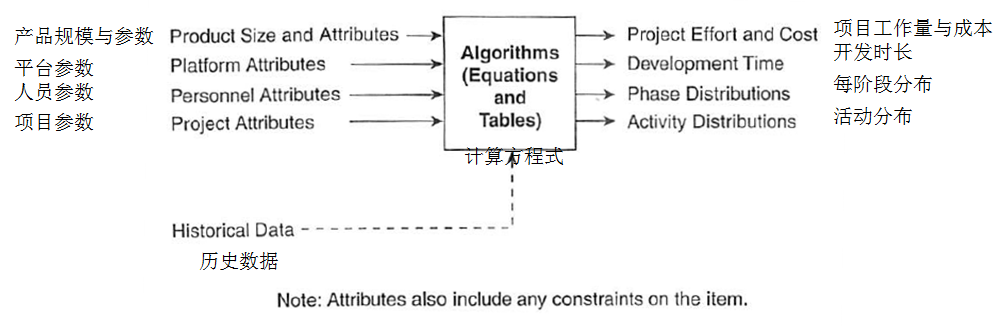
\includegraphics[width=6cm]{估算3.png}\\

或基于国际功能点的ABC模型,依据功能点数,非功能点数,和其他(例如项目管理),ABC
三部分综合估算总工作量(或成本):

%\href{文件:ABC模型.jpg}{600px}

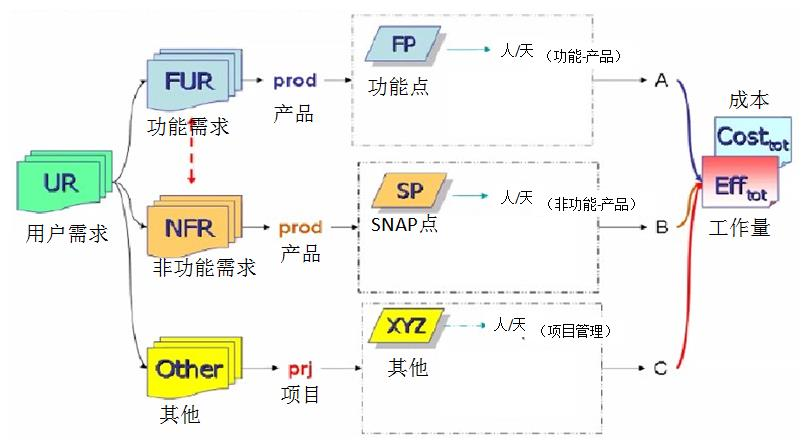
\includegraphics[width=6cm]{ABC模型.jpg}\\

另一方面,专家估算法,例如WBS估算,是以专家主观判断为主(例如,判断活动完成的最可能人天数)。模型估算一般比较客观、可重复性,不像第一种那样主要依赖人的主管判断,但依赖估算专家的能力。

JORGENSEN先生批评模型那派,40多年这么多研究,为什么模型估算还不准确,甚至不如用WBS估算。反过来,BOEHM先生说如果没有模型,整个估算就像个黑盒,无法知道规模、工作量、进度之间的关系,永远靠专家,尤其是在开发的初期,模型特别有用,因为早期需求模糊,无法很准确估算WBS工作量。\\

\framebox{%
\begin{minipage}[t]{0.97\columnwidth}\raggedright
专家估算也有不同的变种,有些纯依赖专家主观判断,有些也会依赖历史数据和检查单,并非仅依赖挑选最佳的专家。有些估算方法,例如,我们一般把扑克牌估算(Planning
Poker)归属于专家估算,但如果最后估算主要依据上一轮冲刺的速度(Velocity)或生产率(productivity),它就更类似模型估算了。

所以虽然模型估算和专家估算看起来有明显差异,但有时候不容易明确区分。下表比较专家与模型估算,总结两种方式的主要区分:

%Screenshotfrom2023-01-0602-48-18.png
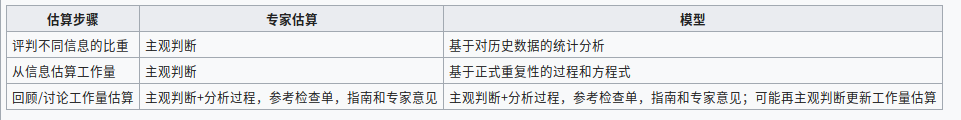
\includegraphics[width=6cm]{Screenshotfrom2023-01-0602-48-18.png}\\

\strut
\end{minipage}}

所以当我们了解为什么不能但靠模型预测,便能理解模型与专家估算,两者各有好处,没有对错,应该两者都要参照。比如模型可以更好地在早期判断,估计整个项目成本,还可以帮我们了解那些因素影响工作量(进度),需要注意。\\

\hypertarget{ux4e3aux4ec0ux4e48ux4f30ux7b97ux5f00ux53d1ux5de5ux4f5cux91cfux5de5ux671fux8fd9ux4e48ux56f0ux96be}{%
\subsection{为什么估算开发工作量/工期这么困难?}\label{ux4e3aux4ec0ux4e48ux4f30ux7b97ux5f00ux53d1ux5de5ux4f5cux91cfux5de5ux671fux8fd9ux4e48ux56f0ux96be}}

你可能会质疑以上的都是大学教授基于学术研究的结论,
实际上数学模型的估算不一定比专家估算差。 我们可以回顾美国SIT的
项目管理估算模拟实验。\\
软件项目管理学生用各种方法估计完成某乐高积木的时长,利用项目数据得出的预算模型的估算准确度还不如戴尔菲法专家估算。(详见附件)\\
由于软件开发很依赖人,主要靠人来做,导致影响生产率的因素很多,如积极性,经验,工具,团队合作等等。用数据挖掘,机器学习,更适合研究一些科学的问题
(物理/化学/生物,如药品的化学成分),相关因素,效用等都好衡量,但是人的因素就没有这么简单。所以过去虽然有几十年的关于工作量的估算模型建立,但准确度一直不太理想。反过来,也不能单靠专家估算,它非常依赖专家的选择,因为人是主观的。虽然主观有可能能帮助做好判断,但也正因为人的主观性,导致估算的偏差。例如,某人做某类软件开发很有经验,她能更准确地估出这类开发的工作量,但如问她能否用一条方程式表达出来,她肯定不知道。\\
所以,如想做好软件开发的工作量估算,首先要理解估算本身的偏差会很大,影响因素很多,也因为无法预测所有(尤其是跟人相关的因素)的影响,个人经验就可以补充估算的不足。

\hypertarget{ux4f30ux7b97ux8f6fux4ef6ux5f00ux53d1ux7684ux56f0ux96be}{%
\subsection{估算软件开发的困难}\label{ux4f30ux7b97ux8f6fux4ef6ux5f00ux53d1ux7684ux56f0ux96be}}

我们有哪个软件开发像玩乐高积木这么直接简单?例如:

\begin{itemize}
\tightlist
\item
  有明确固定的答案;也有明确的步骤,可以照着,按部就班完成
\item
  如果中间过程有错,很容易可立马看出来
\end{itemize}

但软件开发往往是:

\begin{enumerate}
\tightlist
\item
  需求和规范经常有变动(
  大家有哪个项目,需求制定后,到最后开发完成,中间没有变化?)
\item
  软件开发写错一句代码可能影响全盘
\end{enumerate}

因软件开发往往需求不定,所以敏捷大师们反对传统项目估算方式 -
需求(规模)是固定,估算出对应的工期与工作量,并制定整个项目计划与进度表,然后监控,确保项目没有超出计划工期/工时。他们觉得这种以计划驱动的传统管理模式直接影响软件开发团队的生产效率,太多项目因为经理都只是管是否按期完成,是否没有超人时,不考虑软件开发的质量是否给客户价值,反而影响到很多软件项目都被用户诟病。

\framebox{%
\begin{minipage}[t]{0.97\columnwidth}\raggedright
在香港讲敏捷课时,某学员听完敏捷精益的概念后,说她经理要求他她一个三个月的详细工作任务分解,活动详细到五天之内,因为她的经理按计划管理的思路很重。她就很困惑,软件开发变化这么多,怎么可以做出这种详细计划呢?\\其实有点像我们要在一个足球赛还没开始之前,要预先写赛后报告一样没意义,都是猜。\\ 我就回应他说:如果老板有这种思路的话是无法推动敏捷的,其实敏捷有一个很重要的概念,因为需求变化这么大,我们的范围是不固定的,所以基于精益的概念,我们就按有限的时间,制定这个冲刺在两周里面可以完成哪些?做完以后才依据过去的数据进一步策划下一个阶段就更实际了,不是全都靠猜测。这种思路更能让客户尽早看到实际的项目进展,所以敏捷特别重视可以运行测试好的故事,而不是一堆需求文档或者没测试过的代码,因为需求没有给客户看过,还不算是完成,只是一个中间的状态。所以如果经理有这种知道软件开发的特性后,就在那个策划的三角形------时间、成本和规模范围适当取舍,比如,如果我们规定时间为两周,应该可以在那些故事里面挑选最有价值,可以在两周做的故事并完成,展示给客户。就有MVP最小有价值的产物概念,这种就会避免团队为了只追求进度,导致最后做了一大堆没价值的东西,并且很多都没测试好,不能运行。
\strut
\end{minipage}}

我然后跟她说下面这谷歌故事:

\framebox{%
\begin{minipage}[t]{0.97\columnwidth}\raggedright
%\href{文件:Google_Agile_stories_V12esFinal(engCh)v12.png}{600px}\\
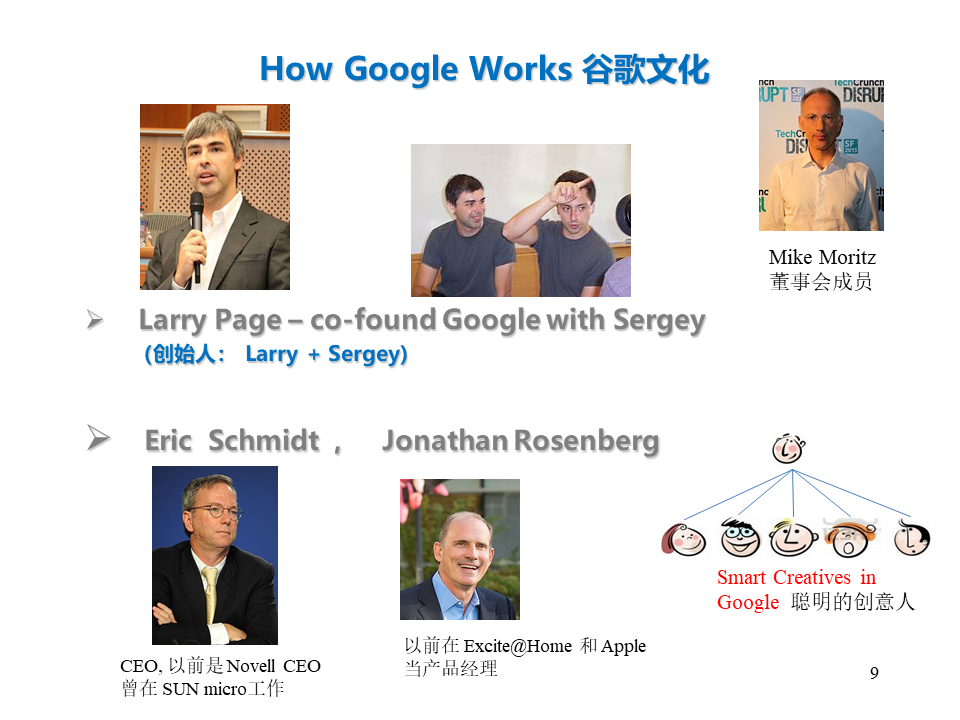
\includegraphics[width=6cm]{Google_Agile_stories_V12esFinal(engCh)v12.png}\\
例如2000年,当时谷歌(Google) 还是很小的公司,但因在搜索引擎有突破,
预计会被微软攻击和收购。

刚进公司的CEO Eric 和 产品经理 Jonathan 便准备了一个详细的两年商业计划。
创始人Larry 看了,便立马问他们俩: ``你们以往有试过超出你们的计划吗?
如果没有,建议还是先跟我们那些工程师聊聊吧。''

后面他们发现Google的工程师都是精英, 无论技术或业务方面的能力都很强,
都有很多创新思路。 了解如果还是按传统的计划驱动反而会
限制了团队的创新能力。\strut
\end{minipage}}

如果团队有能力,应让团队自主创新,传统计划反而会局限了团队发挥,是敏捷开发核心思想。

\begin{itemize}
\tightlist
\item
  因为每次只估算后面迭代(两到四周)的工作量,偏差不会太大
\item
  因为只估算本迭代需求相关工作,减少需求变更的风险
\end{itemize}

因为按范围估算软件开发工作量很困难,
所以只能按有限的资源和时间,识别哪些对客户最重要的功能,
估计能否在项目交付期限内完成。
如果不能,再按功能对客户的价值,选择那些较低的功能可以先不做。

传统项目管理假定规模是固定; 敏捷开发反过来, 时间和资源是固定,
但生产率是按依据团队前面迭代速度的数据。

%\href{文件:微信图片_20230105131327.jpg}{500px}

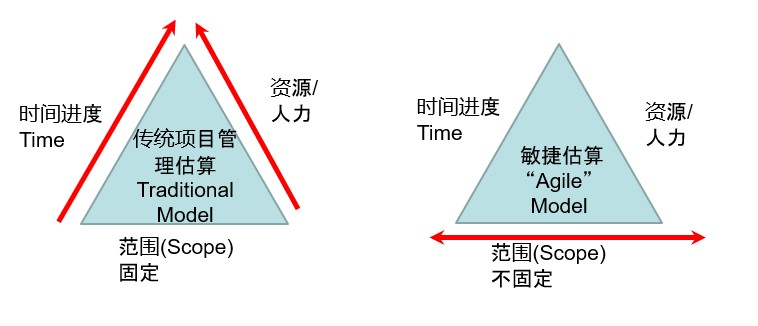
\includegraphics[width=6cm]{微信图片_20230105131327.jpg}\\

这个时间固定,但范围可变的思路,不仅仅适用于软件开发。例如,准备必须月底前将整本书全部交稿,草稿中有不少小错误,如果要全部都修正好,肯定不能按月底期限交付,所以就需要把一些可以删掉的部分删掉,确保书的质量,也把影响降到最低。与软件开发不同,书可以比较轻松删掉一两段,但软件之间的耦合性比较大,可能删掉一行语句整个程序就跑不通,所以更需要在交付前规划好开发的范围,最终才有机会可以按期交付。

敏捷是依据精益MVP概念,时间(资源)固定,范围可变,如果估计不能在交付期限前完成所有客户需求,便要尽早跟客户协商,选择哪些功能放在这次交付之内,哪些放在后面,希望有限的时间和资源条件下,给客户提供最高价值。

很多敏捷团队会用以下方式逐步做估算:\\
先把所有客户的需求写成故事卡片,作为整个项目的交付物(Backlog),然后按每次迭代(例如从第一次迭代):

\begin{itemize}
\tightlist
\item
  先挑选最重要的故事,放在本次迭代,估计相关的故事点,故事点是一个简单的规模概念,团队按照类似的模块的工作量,估计每故事的故事点数(例如,可以用扑克牌举牌方式多轮估算,最终得出一个团队都赞同的故事点数)
\item
  按本迭代可允许的人天数估计本迭代可以完成多少个故事点
\item
  然后每次迭代结束后记录完成多少故事点,形成燃烧图(burndown
  chart),看功能点的降低速度来预估整个项目最终完成的时间,需要多少个迭代。从燃烧图,故事点减少的速度计算项目速度(velocity)。
\end{itemize}

\begin{description}
\item[]
\begin{description}
\tightlist
\item[]
+ + +
\end{description}
\end{description}

有些敏捷大师甚至反对估算(NoEstimate),觉得估算只是凭个人拍脑袋、凭经验,没有依据,反而导致团队只关心进度不能延误,影响开发员,使得开发人员反而不能专心专业地做好软件开发。\\
NoEstimate反对使用故事点估算,故事点按个人经验来估算,不同人的理解不一样,可能导致差异很大。同样,他们也反对敏捷Velocity速度的概念,觉得只是另一个形式的传统策划思维,也会导致团队只是关注一个冲刺迭代交付了多少个故事点,反而忽视了交付的软件是否对确实客户有价值。\\
但他们也理解到团队还是要可以预估可否在客户定的期限件内交付,或者交付多少,因为这是客户关注的。他们建议直接把backlog里要交付的所有需求,细分成小故事,每个故事最好是一人天左右。这样就很简单,可以按完成故事的速度,更客观地预计客户要最后交付的日期(例如,十周后),可以完成多少故事。\\
例如,共要求300个故事,按团队速度,十周后只能总共完成200,就要提前按优先级、重要性跟客户协商,挑选哪些在这个期间前交付,那些放到下一次再做。(前提是:团队必须已经做了一些开发,知道每次两种迭代大概可以完成多少故事。)

\hypertarget{ux603bux7ed3}{%
\subsubsection{总结}\label{ux603bux7ed3}}

选择那种方法估算软件开发工作量,跟选择最合适的项目生命周期方法类似,取决于项目的特性和团队的能力。
如果需求很明确和固定,可没有客户代表在每个迭代(2-4周)确认,例如,政府投标定制开发项目,就不一定选择精益MVP思路的敏捷估算方法,而应依据范围(scope)和规模(size),估算工期与工作量,除了使用WBS分解从下而上靠专家/团队估算工作量与工期外,也要利用规模(功能点数),利用基于历史数据的估算模型从上而下估算。(千万不用以为那种估算最准确,其实都不准,但综合考虑可以减少偏差)

如果需求很可能会变,客户参与,团队能力强的产品性开发项目,时间/资源固定,范围可变的精益敏捷
思路就更能为干系人创做价值。如果可以把范围细分到很小的估算(每故事
\textasciitilde{}1人天),可以依据以往历史速度,估算要完成所有需求一共要多少次迭代(或周);但如果项目复杂,之间相互依赖,有些模块要多人合作,难以细分,就难以用前面的简单线性估算,须要团队估算工作量,但不应只依赖从下而上按任务估计工作量,也要参考规模大小,利用估算模型从上而下估算,然后综合考虑。

%\href{文件:敏捷非敏捷1.jpg}{400px‎}

\includegraphics[width=6cm]{敏捷非敏捷1.jpg}\\

\hypertarget{ux9644ux4ef6}{%
\section{附件}\label{ux9644ux4ef6}}

\hypertarget{ux4f30ux7b97ux780cux4e50ux9ad8ux79efux6728ux65f6ux957f---2015ux5e74ux5b66ux751fux5b9eux9a8cux6570ux636e}{%
\subsection{估算砌乐高积木时长 -
2015年学生实验数据}\label{ux4f30ux7b97ux780cux4e50ux9ad8ux79efux6728ux65f6ux957f---2015ux5e74ux5b66ux751fux5b9eux9a8cux6570ux636e}}

2015年,17位有工作经验的兼读学生
参加SIT的软件估算与度量课程(一个学期,共13节课)。
为了让学员亲身感受软件估算的困难,
老师要求学员用以下各种方式估算要完成乐高"Sopwith
Camel"积木(详见下图)的时长:

%\href{文件:Lego1.jpg}{300px}

\includegraphics[width=6cm]{Lego1.jpg}\\

\begin{enumerate}
\tightlist
\item
  每位学员独自做估算 (I)
\item
  使用戴尔菲法(Wideband Delphi),多轮后更新(个人)估算 (II)
\item
  分成3组,每组也使用戴尔菲法,制定本组的(团队)估算 (II(团队))
\item
  依据实验数据(注2)调整、更新(个人)估算 (III)
\item
  团队也依据实验数据调整、更新(团队)估算(III(团队))
\item
  完成以上4、5步后,立马告知会选那位学员实际做LEGO积木(注3),让个人调整、更新(个人)估算
  (IV)
\item
  也让团队调整、更新(团队)估算 (IV(团队))
\end{enumerate}

\framebox{%
\begin{minipage}[t]{0.97\columnwidth}\raggedright
注1:

\begin{itemize}
\tightlist
\item
  之前在课程里,已正式学过戴尔菲法
\item
  加上规模,复杂度等对工作量、生产率的影响
\end{itemize}

注2:
让学员自己做乐高实验(因有些学员可能从未玩过乐高积木),提供4对同样的积木:

\begin{itemize}
\tightlist
\item
  Big Ben(下面有完成后的照片)
\item
  Leaning Tower of Pisa
\item
  Eiffel Tower
\item
  General Grievous Wheel Bike
\end{itemize}

%\href{文件:Lego_2.png}{300px}

\includegraphics[width=6cm]{Lego_2.png}\\

\begin{itemize}
\tightlist
\item
  每学员记录实际完成的时长,把所有数据汇总并公开给所有人
\item
  之前在课程里,已正式学过预测模型和数据统计基础,如何利用以往数据,建立模型(附件里有如何建模的介绍)
\end{itemize}

注3:

\begin{itemize}
\tightlist
\item
  大家都有这位学员之前乐高实验所需时长的数据
\end{itemize}\strut
\end{minipage}}

\hypertarget{ux5b9eux9a8cux7ed3ux679cux4e0eux8ba8ux8bba}{%
\subsubsection{实验结果与讨论}\label{ux5b9eux9a8cux7ed3ux679cux4e0eux8ba8ux8bba}}

%\href{文件:Lego3.jpg}{600px}

\includegraphics[width=6cm]{Lego3.jpg}\\

\begin{itemize}
\tightlist
\item
  那学员用了213分钟(差不多3.55个小时)完成,他自述困难主要在于颜色都很类似,很多时候找不到合适的积木。(跟其他体验组比较,其他2-3
  组都差不多在210 - 220分钟范围之内完成)
\item
  戴尔非法显著减少了个人估算的偏差,用戴尔菲的团队估算其实是最接近实际的,估得最好的,偏差不超过15分钟。开始时,尤其个人都会多估,但后面数据越来越多,反而开始有点偏低了
\item
  可能导致后面估算偏低的原因:之前实验用的4组积木都是建筑物,复杂度与颜色搭配都较简单
\end{itemize}

\hypertarget{ux7ecfux9a8cux6559ux8bad}{%
\subsubsection{经验教训}\label{ux7ecfux9a8cux6559ux8bad}}

\begin{enumerate}
\tightlist
\item
  学生经过这个过程可以从实验亲身感受到估算的局限,没有想象这么准确,太多因素影响,也很难建立一个预测模型,比如偏差可能到了0.3以上
\item
  从这个过程里面也让他们感受到主观判断的重要性,不要以为仅仅客观用一些数据、用数学方程式就可以准确估出正确的答案
\item
  也了解复杂度和人对生产力的影响,比如积极性跟经验都是很重要的因素。例如,有一个学生经验很少,但竞争力和积极性非常高,所以有好的成绩。有两个团队也是完成同一套??模型,发现本来自己判断为高经验的团队反而比中经验的团队花多一倍时间,最慢的团队是一个两人团队,因为基本没有经验,所以就很小心,一步一步去做,尽量少减少错误,导致用的时间最长。
\item
  团队规模大小也有影响,团队人数越多其实是对整个生产力有负面影响,人数少反而会好一些。(其它关于软件开发的研究也有类似的发现)
\end{enumerate}

很多人以为软件项目估算与其他项目(如土木)类似。以上实验,虽然不是真正做软件开发,学生自己做估算,从亲身体验学习,
更好了解软件项目估算的常见误解:

\begin{enumerate}
\tightlist
\item
  以为软件估算可以精确到正负几个百分点
\item
  以为在项目时间不够的时候,增加人员对项目的进度会有帮助
\item
  以为团队人越多,工期就按比例缩短,像建筑工程一样
\item
  以为估算是可以单靠一些预测模型简单地估出一个数值。
\end{enumerate}

学生都没有软件项目的经验,我们也不可能在上课的时候做软件项目,于是用乐高积木,让他们做估算,比如我们让他们依据一个结果图,估算要多少人时来完成积木,也要看人的乐高经验,首先第一步是他们单独做估算。我们在课程中用了Wideband
Delphi 估算法,每个人多轮估算。找人确实来建乐高,看看实际用了多少时间。
然后我们在课程中加了一些估算模型,用一些历史数据给他们进行参考,下面就是我们的一些发现:很多人在没有经验的时候都会高估,用了Wideband
Delphi 的方式会确实比较准确。
后面有了实际数据,要求学生利用软件项目估算模型方式来估,他们就发现这不容易,很多时候,有学生直接改用简单方程式做估算。
学生自己动手来估算,才会有感觉,真正了解软件估算的各种困难。\\
%Screenshotfrom2023-01-0602-54-00.png
\includegraphics[width=6cm]{Screenshotfrom2023-01-0602-54-00.png}\\

注:上面 I,II,III,IV 与 下面 II,III,IV
的定义,对应那种场景,已经在上面本文里说明。

%Screenshotfrom2023-01-0602-54-26.png
\includegraphics[width=6cm]{Screenshotfrom2023-01-0602-54-26.png}\\


%Screenshotfrom2023-01-0602-55-33.png
\includegraphics[width=6cm]{Screenshotfrom2023-01-0602-55-33.png}\\
注:偏差 MRE(Magnitude of Relative Error) = \textbar{} (实际 - 估算)
\textbar{} / 实际

\hypertarget{references}{%
\section{References}\label{references}}

1. JORGENSEN, Magne . B. BOEHM: "Software Development Effort Estimation:
Formal Models or Expert Judgment? " , IEEE SOFTWARE, March/April 2009\\
2. LAIRD, Linda, Y. YANG: "Engaging Software Estimation Education using
LEGOs: A Case Study" 2016 IEEE/ACM International Conference on Software
Engineering Companion\\
3. DUARTE,Vasco: \emph{NO ESTIMATES: How to Measure Project Progress
without Estimating}\\


%done-1



\part{利用评估开始过程改进}团队必须先获得管理层的关注与支持\\

%\part{利用评估开始过程改进\\ \textbullet \textbullet \textbullet \\团队必须先获得管理层的关注与支持}

%\chapter{获取高层支持} % Introduction chapter suppressed from the table of contents

我:对于过程改进来说,最重要的成功要素是什么?\\
客户:最难的是如何得到高层的支持,这不仅仅是嘴巴说说而已,而是要切实地给人、给时间。高层往往不清楚什么是质量改进的重点,但他们对员工的人均收入、利润(比如员工可为公司盈利的时间占比多少?如果少,就表示这个员工对公司的盈利贡献不够。)等这些财务指标都非常清楚。\\
我:非常赞同。我们可以利用评估机会来引起高层对质量改进的重视,但往往评估组只说软件开发的各种问题,难以引起他们注意。一般人,尤其是高层,一听到问题都会觉得比较烦,没有动力听下去,更不要说有对应的改进行动了。\\
客户:你说的挺有道理的。确实我们每年都会有一些评估,发现了不少问题。高层也都会参加评估会,并同意这些问题需要改进。但很多时候过后就没下文了。\\
我:质量大师Dr. JURAN
有丰富的过程改进的经验,他深知要说服高层真心投入、支持改进,就必须用高层的语言打动他们。如果与高层交流,不能把团队关注的事转化成高层关注的,就难以获得立项,做改进。

我:所以在最近的评估里,我会引导公司内部的评估组成员,通常是公司的PMO或QA,跟发起人(公司高层)汇报时,着重汇报关于如何改进、为公司节省成本的初步方案。你要兴趣听听这案例吗?\\
客户:非常有兴趣。\\
%==案例 ==
\hypertarget{ux7b2cux4e00ux7248ux65b9ux6848ux4e66}{%
\subsection{案例}\label{ux7b2cux4e00ux7248ux65b9ux6848ux4e66}}
我问公司内部评估组,高层有哪些关注点?他们就列出来,如人均收入,人均利润等商务指标。\\
然后我再问影响这些指标的因素很多,有些是软件开发团队无法控制的,例如销售人员与客户的关系,所以我们必须从这些高层关注的指标细分到一些团队实际可以影响到的指标。有哪些呢?\\
评估组:项目进度的偏差,遗漏给客户的缺陷数。\\
我:这些我们都叫性能目标。这些指标是如何影响高层目标的?\\
评估组:比如项目延误,成本就会超支。\\
我:是的。如果我们过程改进希望改善质量、减少缺陷,你们觉得会对成本有什么影响?\\
评估组:改进要投入工作量,肯定会增加成本。但长远应可能降低成本。\\
我:很多高层都不熟悉质量管理,所以很少关注和监控团队的缺陷。他们通常还是会觉得质量改进是好事,但要花成本。我做到客户满意的水平就可以了,不要追求十全十美,也正是这个误解,才导致他们认为大部分缺陷在系统测试或验收阶段才发现是正常的,是常态。如果是做软件产品的公司会好一些。我们在前面迭代回顾里面解释了,尤其在软件工程领域,因为缺陷发现越靠后,返工工作量是在前面发现的同样缺陷的几十倍。所以如果我们能把返工缺陷预先发现并处理,必然会大量降低返工工作量,与相关成本。\\

\hypertarget{ux7b2cux4e00ux7248ux65b9ux6848ux4e66}{%
\subsection{第一版方案书}\label{ux7b2cux4e00ux7248ux65b9ux6848ux4e66}}

小李做了第一版的方案书。\\
%\href{文件:方案书1.jpg}{600px}

\includegraphics[width=10cm]{方案书1.jpg}

我:小李,挺好的。你在投资方面是保守型吗?\\
小李:不是啊,我还会定期买股票,因为单是靠银行定期,利息太低了。\\
我:但是看你在质量改进方面的目标很保守。比如你看,说如果做了改进以后,后面的缺陷可以降低百分之十到百分之二十,然后最后算出来节省不到五个点。你估计高层会买单,投资你这个项目吗?\\
小李:确实有道理。\\
我:你这里有几个地方没做对,例如从我们过去的经验,因为很多团队在前面几乎没做好单元测试或代码扫描,反之,系统测试或者验收测试的缺陷几乎可以减少一半。低的目标不是好目标,还有,你评估在后面阶段返工的工作量也太低了,只是比前面发现的高一点点。你尝试依据这两个思路再调一下吧。\\
小李:你有所不知
,我们虽然有些行业参考数据,但没有实际项目数据支撑,是否需要先找些实际数据才可以做方案,不然好像说不过去。\\
我:在初步方案阶段,其实不需要实际数据的支撑。你可以想象,目的是要让管理者有依据做决定,如果你想利用数据把这些数字做得更准确,这对高层的决策没有实际帮助。所以在初始阶段,合理的估算就足够了,不需要花精力在没有价值的事情上。\\

\hypertarget{ux7b2cux4e8cux7248ux4e0eux4e2dux5c42ux786eux8ba4-ux7136ux540eux5411ux9ad8ux5c42ux6c47ux62a5}{%
\subsection{第二版与中层确认,
然后向高层汇报}\label{ux7b2cux4e8cux7248ux4e0eux4e2dux5c42ux786eux8ba4-ux7136ux540eux5411ux9ad8ux5c42ux6c47ux62a5}}

做了第二版后,我们再跟中层确认一下,他们觉得这个也确实比之前更有说服力了。建议中层除了数字以外,如果能配上一些柱状图,可以让听众(高层)更容易理解。\\
%\href{文件:!!JiangJingFinal2presentScreenshot_2022-09-12_092535.jpg}{600px}

\includegraphics[width=10cm]{JiangJingFinal2presentScreenshot20220912092535.jpg}

小李跟高层汇报,并得到高层的认可后,高兴地说:以前都以为过程改进应先自己默默耕耘,先在试点取得效果,再跟高层要资源,再推广,现在看,还是应该一开始便提具体改进方案,并立项,才有机会成功。\\
我:管理层是过程改进最重要的干系人,必须一开始便得到他们支持。你后面有什么计划?\\
小李:既然他们都同意,我就开始找项目开始试点,对吗?\\
我:应该马上制定详细的计划,包括团队分工,否则你的改进方案还是难以落地。\\
小李:你说的有道理,我马上今周做,然后发他们邮件跟进。\\

\framebox{%
\begin{minipage}[t]{0.97\columnwidth}\raggedright
\hypertarget{ux53cdux9988}{%
\subsubsection{反馈}\label{ux53cdux9988}}

某CTO:
方向很好,但高层关注的不只是销售额这些商业指标,还有交付效率和质量的指标。\\
公司老板针于研发除了关注成本外,也关注:

\begin{itemize}
\tightlist
\item
  人员:人均薪资、人均产能、人员参项率(有收入的项目)、人员闲置率
\item
  进度:是否能正常交付
\item
  质量:缺陷率、严重缺陷数
\end{itemize}

举例说明:比如提升效率这样的指标,多数公司都用人均产值,人均交付金额这些指标。但大多数公司没有想过创新,如果公司业务很稳定,那么针对重复性工作是否能形成公共组件或低代码平台,来大幅度提升生产率。再说质量方面,如果客户能参与使用,例如,产品定义,需求的质量会大幅度提升(不仅依赖评审,测试)。对于这个逻辑,凡是做过程改进的人都能理解,但为什么客户不愿意深度参与,是因为没有让客户可以高效参与的工具。\\
例如,90\%以上的公司都是靠需求文档,RP原型的方式沟通需求,效率不可能高。但如果低代码平台能快速形成需求和客户可体验的需求,效率和质量都会大幅度提升。

我:
过程改进想要成功,首先必须得到高层的支持,但团队往往只关注日常任务,高层不一定懂质量,所以必须靠中层作为高层与下面团队的桥梁,把质量改善简化成高层可以理解的方案,让他决策。\\
%::\href{文件:三角形.jpg}{400px}
::\includegraphics[width=10cm]{三角形.jpg}
上面这案例,高层只关注财务指标,没有任何质量或创新的度量指标,虽然我们都知道单靠财务指标是不全面的,但也只能用财务数据。但如果面对像你这种通情达理的高层,就可以更全面,从质量、创新等多维度估计改进可为公司带来的价值。\\
\strut
\end{minipage}}

\hypertarget{ux603bux7ed3}{%
\subsubsection{总结}\label{ux603bux7ed3}}

从以上简单案例,得到的经验教训:\\
1.评估是接触到高层最好的机会\\
2.但评估往往只是针对具体的问题,对不上高层关注的方向,难以获得实际支持\\
3.在做改进方案时,只需要估算,暂时不需要实际数据,以此可以节省资源和时间\\
4.如果确实有高层真正支持的话,就必须正式立项,再配上具体的团队、分工和详细计划,否则整个改进计划还是一纸空文\\



%done-1
%\chapter{利用评估寻找改进机会} % Introduction chapter suppressed from the table of contents

客户:如果想改善我们的敏捷过程,但没有概念,应该怎么开始?\\
我:可以借用评估,例如CMMI评估。\\
客户:CMMI不是和敏捷打对台吗?\\
我:这是很多人的误解,把CMMI等同于瀑布式开发,而且误认为CMMI评估只是一项认证。本来CMMI的目的是帮助企业,例如美国国防部,评价自己和供应商的软件开发过程质量,诊断软件工程软件开发过程有哪些不足。所以CMMI
很全面地覆盖项目管理,软件工程等领域。

敏捷过程,例如 SCRUM, XP
等都能对上大部分的CMMI实践。但反过来敏捷的实践只包括部分CMMI实践,不全面,例如缺少组织级部分,最新的V2.0
版本更精简,更适合敏捷团队。\\
客户:怎么可以利用CMMI?学习一下资料就可以了吗?\\
我:这也是很多团队的误解,跟培训学习的道理一样,若只是吸收了知识,没动手动脑筋,不会有什么作用。我刚开始做CMMI评估时,有些企业说:''CMMI是挺好的,但我们不需要花这么多钱、精力去做评估,平时自己学习一下就可以了,我们很厉害的。``但过了六个月、或一两年后,再次拜访客户,99\%概率,后面一点改进都没有。所以评估本身就是改进的驱动力、再配合评估,作为过程改进的里程碑,使团队有集中改善的压力。你可以想象如果没有评估的话,大家都忙,那里会有时间与动力回顾并改善平常于平常习惯了的做法。(可参考附件案例,了解CMMI评估如何帮助项目组提升)

但请注意,虽然评估能帮我们识别出一些改进点,但过程改进必须以项目来驱动。\\
客户:请解释一下。\\
我:首先要理解纠正措施(corrective action) 和改正(correction)
的区别。这一点我刚开始接触CMMI的时候,已经听过,但没有了解。

\begin{itemize}
\tightlist
\item
  改正Correction只是针对问题的表面,去处理,不能长期避免同类问题再发生。
\item
  纠正措施Corrective action
  是对利用差距分析的数据或者发现,探索背后的根因做计划,针对原因作纠正措施,并制定详细的改进计划,对应我们说改进都要有以一个项目的形式做起一样。
\end{itemize}

CMMI里面一直都有这条实践,但很多时候团队只是像平常解决问题一样,只做correction,对真正可以长久的改进没有任何帮助。所以对评估发现的问题,不应仅仅做个问题跟踪表,一一解决,更应该利用二八原则,找出识别出最有效果的改进项目,然后以项目方式去改进。如果只是做correction,人做事习惯没有变化,后面那些问题还是会重复出现。\\
客户:你说的好像还是挺有道理,是否可以举些例子。\\
下面就举一个关于组织培训的实例:\\
%==评估中访谈公司培训专员==
\hypertarget{ux603bux7ed3ux8bbfux8c08ux7684ux95eeux9898ux53d1ux73b0}{%
\subsection{评估中访谈公司培训专员}\label{ux603bux7ed3ux8bbfux8c08ux7684ux95eeux9898ux53d1ux73b0}}
评估师:请问你们如何与上级和管理层汇报公司培训的情况?\\
培训专员:我们每次都有培训报告,内容包括学员的考试成绩、反馈、出席情况等。也有每年的总结报告,包括整年所有的培训,比如实际与计划对比,费用与预算比较等等。\\
我:是否可以举例?\\
培训专员:例如我们比较关注信息安全。因为很多客户尤其是政府客户也注重这一点,所以我们就找一些外面的培训课,专门对员工做一个线上的信息安全培训。大概有一百个人参加,为了衡量培训效果,老师都会有考试的题库,然后随机考,及格分数线是80分,但是第一轮考试只有六十多位及格,我们就觉得效果不好,就要求那些不及格的重考。第二次的话有一些通过。但还是有二十位左右,第二次还是不通过。\\
评估师:你们觉得效果如何?满意吗?\\
培训专员:不太满意,但后面该怎么做呢?

\begin{description}
\item[]
\begin{description}
\tightlist
\item[]
。 。 。 。 。
\end{description}
\end{description}

评估师:请问你们如何培训新进公司的开发人员?\\
培训专员:我们都有一系列的新员工技术培训课,上午会讲一些原理要求,然后会有一些编码练习,比如如何设计跟开发一个人事管理系统。我们会把用的框架和复用组件放到内网,方便他们获取。也会定好系统的主要模块和相关的测试用例,让他们可以在编程的时候用上那些原则和理论。
评估师:挺好的,你们如何对他们做出反馈?\\
培训专员:我作为老师会对他们的开发进行评价、打分,告知他们不足之处。\\
评估师:是指我们平常年终评价那种,按表现的优秀程度打分吗?\\
培训专员:差不多,我们会从不同的角度去评价。比如我们强调是否按公司的编码规程?是否满足面向对象不耦合原则?从多个角度去评价,进行综合打分。\\

\hypertarget{ux603bux7ed3ux8bbfux8c08ux7684ux95eeux9898ux53d1ux73b0}{%
\subsection{总结访谈的问题发现}\label{ux603bux7ed3ux8bbfux8c08ux7684ux95eeux9898ux53d1ux73b0}}

单是处理发现的问题很简单,只要针对每一条制定对应的措施,例如:

\begin{enumerate}
\tightlist
\item
  发现培训反馈靠主观,只是靠老师主观打分,可以加考试就可以满足不客观了
\item
  发现有些课学生成绩及格率低,下一次同类外部培训要求学员备课,以提高学生的通过率,也是一个改正措施
\end{enumerate}

只是采取这些行动,对公司级培训质量改进作用吗?
几乎没有,因为只是对问题做correction,没有改变系统与习惯,类似问题再出现,还是以前的做法。\\
但如能深入探索根因,就发现原来新员工正式上课的培训不长,只有一天,大部分还是靠新员工在工作中,跟有经验``老''员工导师,老带新,边做边学。但因为很多有经验的都忙于做项目,没有时间带领新员工,所以主要依赖新员工自学,导致新员工培训的效果差异很大。\\
也正因为新老员工都没有持续学习的习惯,都是边做边学,导致参加比较正式的课程前,没有备课的习惯,导致及格率比较低。也发现原来公司有给客户开发并提供线上学习平台。\\
评估师问:为什么没有类似的用于内部的平台?\\
公司总监:平台我们是有的,但是没有课件。我们工作也很独特,没有一些可以买回来的培训可见可以用。所以就一直都没有计划用这个平台。\\
评估师解释说:现在很多公司,尤其疫情原因,都倾向利用培训平台帮助员工学习,虽然没有传统面对面的培训效果好,但肯定会比自学好多了,同时还有上课记录、考试等度量。但是要做到这样,公司肯定要花时间、精力去准备课件,才真正对公司级培训有长久的改进作用。\\
后面总监在评估后,与大家讨论这个评估的发现,大家都同意这做法会有帮助,并且评价这个改进项目的投入和价值,最终成功立项,作为下半年的主要改进项目之一。\\
客户:听完你这个例子,回顾一下我们每年都会有各种评估,但只是针对每一个发现的问题做一些修正,确实对整个公司的质量没有任何提升的作用。大家做事的习惯还是一样,把评估和处理问题当成一些常规性应付的工作。

%\href{文件:IssuesScreenshot_2022-10-19_205655.jpg}{600px}

\includegraphics[width=10cm]{IssuesScreenshot20221019205655.jpg}

我:所以我们说要有真正的质量改进,必须针对弱点找出根因,变成一个改进项目去做才有效果。所以,如果希望可以利用评估改进,首先大家的心态要改过来,如果只追求通过评估的心态,只给评估组看最好的一面,尽量不让问题暴露,对公司的质量改进其实没有作用。但是反过来,如果大家希望这些模型能帮助发现不足,识别改进的机会,评估可以很全面地帮助我们,就好像去医院做体检一样,各方面都会帮我们看。所以每次评估时,我都会让大家放心,千万不要担心问题被发现,我们发现的问题都不是个人或者项目组的问题,都是系统的问题,系统有不足,才导致有这些问题发生。所以每次评估也必须遵守保密跟不追究原则,让大家可以放心说出不足,才可以起改进的作用。

所以评估可以帮助企业全部诊断,找出可改进的点,但如果没有用上根因分析,转化成过程改进项目,质量还是不会改善。有些团队以为用了鱼骨图,找出一些改进措施便是做了根因分析,可看看下面:

\framebox{%
\begin{minipage}[t]{0.97\columnwidth}\raggedright
你说我们团队没有找出真正根因,不理解根因分析的核心,我非常赞同。日本软件开发在根因分析做得特别好,我之前在日本工作,带领小组做开发,当时我们团队共5人,有2位来自大陆,其他是本地人,有一次,因为我们开发计算公积金出错,QA一直追问问题的原因。当时我还没有找出根因的概念,不明白QA的意图,以为只是问责,希望找个人背锅。其实他们确实是希望找出问题的源头,避免同类问题再发生。当主管追问原因,要求我发问题报告。我的报告只说了一些开发问题,人员经验不足等。主管一直追问为什么。例如
``如果你说培训经验不足,你有什么培训相关的安排来避免?''我回答不上来。最后发现,原来是日本计算方法和大陆不同,他们不四舍五入,导致我们两位大陆开发人员的计算便和本地的不同。
很多大陆工程师没有根因分析概念,认为质量依靠个人保证 -
``我负责,有问题我承担''。日本人不是这个思路,他们希望挖掘到问题的根本原因,并避免。\strut
\end{minipage}}


\hypertarget{ux7ba1ux7406ux5c42ux7684ux7406ux89e3ux4e0eux652fux6301}{%
\subsection{管理层的理解与支持}\label{ux7ba1ux7406ux5c42ux7684ux7406ux89e3ux4e0eux652fux6301}}

评估发现会分成弱项与建议两类:

\begin{itemize}
\tightlist
\item
  弱项是指跟模型的要求有明显差距
\item
  建议比弱项程度轻,没有明显差距但可以改善的点\\
\end{itemize}

因评估过程要求标弱项要得到大家,包括内部评估组成员认同,但某些内部评估组成员对弱项就特别担心,尽量想办法解释。有些弱项可能要反复讨论十几二十分钟,他确实没办法才接受。

"我们理解你说项目量化管理计划模板中写公司基线的地方应该是公司目标,公司目标里应该是写总体的年度目标,我们同意模版有不足,应该后面改善,但应该算是建议,不能当成弱项。"

但是如果提建议类的,一点问题都没有。为什么发现弱项跟建议反应区分这么大呢?
后来发现,原来领导关注评估,看弱项多少,觉得如果弱项多就表示相关人没做到位,但恰恰是管理者这种心态妨碍了企业的过程改进,因为要改进,首先要觉得本身有不足,才有动力挖掘不足的根因并做改进。

评估师问:您觉得你们配置管理做得如何?有没有一些你不满意的地方?\\
研发总监:挺好的。没有问题。\\
(但实际上,从文档检查已发现在配置审计、建立基线、基线变更、如何保证文档、环境配置与代码同步等都有不足。)

所以如果想利用评估来做改进,首先管理者要觉得本身有不足,并理解评估的目的,就好比我们做代码走查,如果没发现是坏事一样道理。

如想多了解应如何分析根因,并在敏捷项目中使用,例如冲刺回顾,请看下部分"从做好迭代回顾开始”。

%\subsection{总结}\label{ux603bux7ed3}}

\hypertarget{ux9644ux4ef6ux6848ux4f8b}{%
\subsection{总结}\label{ux9644ux4ef6ux6848ux4f8b}}

CMMI 过程改进的成功要素:\\
\textbf{1.时间}
如果公司希望借用CMMI确实做到一些具体的改进,因为要足够的时间来累积数据,整个项目时间不能太短,比如小于6个月就很难达到改进效果。\\
\textbf{2.计划}
一开始就要做好计划,企业要有过程改进组人员的投入,包括负责度量与分析。而且还要有合适的工具,单靠手工很难收集真正的项目数据。\\
\textbf{3.方法}
培训不仅仅是教CMMI模型,更重要是有一些具体的方法、模板、工具,可以让项目组立马用起来。项目实战辅导很关键,听得懂并不一定会用,老师的实战辅导才能真正将方法落到实处。\\
\textbf{4.使用功能点估算项目规模使项目间可比}
直接从需求估算功能点数,让不同项目的度量数据可比,不然无法建立公司基线。\\
\textbf{5.预测模型}
不仅衡量结果,也要度量过程中的可控因子。例如扫描代码,尽早暴露问题,不用等到系统测试才发现缺陷,减少返工。\\
\textbf{6.工具与平台}
尽量用工具取代人手工作,例如,提供了从需求计算功能点数的模板工具等。\\
\textbf{7.高层的支持}
高层与事业部领导的支持非常重要,可以想象如果他们不认同这些对企业长远的帮助,很难要求他们投入这么多人力资源在这个项目中。
如果领导不关心,很可能评估过后便回复到改进前的状态,不能持续。


%\hypertarget{ux9644ux4ef6ux6848ux4f8b}{%
%\subsection{附件}\label{ux9644ux4ef6ux6848ux4f8b}}

\hypertarget{ux9644ux4ef6}{%
\section{附件}\label{ux9644ux4ef6}}

\hypertarget{ux9644ux4ef6ux6848ux4f8b}{%
\subsection{CMMI评估案例}\label{ux9644ux4ef6ux6848ux4f8b}}


某咨询顾问的回顾:

我们提供wiki服务器,里面除了提供模型、Q\&A问答、视频等,帮助团队了解CMMI的最佳实践。并要求每个项目组按模型的每一条实践,写出是如何在项目组体现。要顺利通过CMMI评估,项目组不仅需要提供数据,也需要参加访谈,把项目的故事讲出来。\\
因Wiki服务器是个交互平台,公司每个人都可以随时访问,所以评估组和我可以随时了解到他们对CMMI
实践的理解是否有错误。\\

%\hypertarget{ux9879ux76eeux7ecfux7406ux4e0eux5927ux5bb6ux5206ux4eabux6c47ux62a5}{%
%\subsection{项目经理与大家分享/汇报}\label{ux9879ux76eeux7ecfux7406ux4e0eux5927ux5bb6ux5206ux4eabux6c47ux62a5}}

\textbf{项目经理与大家分享/汇报}\\

客户完成了CMMI
V2.0评估后,举办项目团队评估后总结会,安排了其中的3个项目团队汇报他们在过去半年,如何利用所学到的方法达到CMMI5级评估要求。
非常高兴地看到他们已经掌握了我们老师所培训的技能------利用模板从需求计算功能点,然后从功能点估算出项目工作量、测试用例数,再利用小工具测量代码质量,并且预估最终的缺陷密度等。\\
3位项目经理每人都针对以上内容发表了的1小时的演讲,分享实战心得。\\
项目团队把学到的东西用于项目中,配合度量数据,取得具体的质量提升,且达到了相应的CMMI评估要求。\\
%\href{文件:000.jpg}{500px}

\includegraphics[width=10cm]{000.jpg}

这些项目经理都非常忙,每天可能工作到晚上十点/十一点;如果没有CMMI五级评估驱动,很难在短短几个月时间内达到这效果。
其他项目组也因为听到有改进效果,产生兴趣专门抽空过来听。\\
过程改进要有效,离不开3个方面的相互配合:培训+评估+自动化工具。\\
%\url{文件:3个关键点图1.png} 

\includegraphics[width=10cm]{3个关键点图1.png}




%done-1

\part{从做好迭代回顾开始 }做好迭代回顾让团队向量化管理迈进一大步\\

%\part{从做好迭代回顾开始\\ \textbullet \textbullet \textbullet \\做好迭代回顾让团队向量化管理迈进一大步}

%\chapter{做好准备} % Introduction chapter suppressed from the table of contents

\framebox{%
\begin{minipage}[t]{0.97\columnwidth}\raggedright
\textbf{请你按过去一年的软件开发项目,按工种占项目总工作量,从最多排到最少?}

\begin{enumerate}
\tightlist
\item
  编码与代码设计
\item
  交付后的所有工作,包括维护、更新与缺陷修正
\item
  交付前的评审,静态扫描,测试与缺陷修正
\item
  项目管理与监控
\end{enumerate}\strut
\end{minipage}}

可看附件中的``开发项目工作量(成本)分布'',看你的选择与`典型'分布差多远。

软件开发项目通常最大的成本是花在找出与修正缺陷。

按专家Capers JONES 先生2012年的研究,
超过10,000功能点,计划能使用25年的大型系统,接近一半的工作量都是与找出与修正缺陷相关。

\begin{description}
\item[]
\begin{description}
\tightlist
\item[]
= = =
\end{description}
\end{description}

初次见软件研发总监,我会问:``通常你们的项目在哪个过程中发现的缺陷最多?''

\begin{description}
\item[]
\begin{description}
\tightlist
\item[]
超过95\% 都会说最多是在系统测试,或验收测试阶段发现\\
\end{description}
\end{description}

%\url{文件:AR1缺陷数.jpg}

\includegraphics[width=10cm]{AR1缺陷数.jpg}

再问:用于测试与缺陷修复的返工的总工作量占整个开发项目多少?

大部分领导都没有概念。

我总结:如果能把后面发现的缺陷,提前在前面预先发现,估计可以节省多少工作量?

\framebox{%
\begin{minipage}[t]{0.97\columnwidth}\raggedright
当我在白板上估算出,如果能把系统测试发现的缺陷数减半,总的工作量会减少,研发成本也会降低,很多总监都会觉得不可思议,因他们一直都已经习惯了后面测试缺陷多,觉得是常态。\strut
\end{minipage}}

\hypertarget{ux7f3aux9677ux6392ux9664ux7387-dre}{%
\subsection{缺陷排除率 (DRE)}\label{ux7f3aux9677ux6392ux9664ux7387-dre}}

%\href{文件:jalote_emm_7.1_1.0.png}{500px}

\includegraphics[width=10cm]{jaloteemm7110.png}

Figure7.1,从需求到设计、编码、单元测试、系统测试、验收,整个开发过程大家都很熟悉(缺陷只会源自需求、设计、编码);需求、设计、编码后都会评审/测试来排除缺陷,但仅仅做评审/测试不一定能确保质量。因为最终验收缺陷数取决于每个步骤能否有效排除当前的缺陷。

所以可以用缺陷排除率(Defect Removal Efficiency DRE)
来衡量测试或评审的效率:

%\href{文件:Ma3_1.0.png}{文件:Ma3 1.0.png}

\includegraphics[width=10cm]{Ma310.png}

缺陷排除率除了可以用于整个项目,包括测试,也可以用于前面评审、扫描等。

\begin{description}
\item[]
\begin{description}
\tightlist
\item[]
= = =
\end{description}
\end{description}

有些人会认为尽早发现并解决缺陷
对质量肯定好,但会耗费工作量,增加项目成本,老板不一定愿意。
其实是反过来,如能在前面预先发现并修正缺陷,
便能减小后面测试和修改缺陷的工作量, 最终只会减少总项目工作量。

%\href{文件:AR1FixVarCostScreenshot_2022-12-10_144400.jpg}{600px}

\includegraphics[width=10cm]{AR1FixVarCostScreenshot20221210144400.jpg}

比较以上两种策略的质量成本(COQ)就能看出:

\begin{itemize}
\tightlist
\item
  增加测试前扫描与审查,并加大测试效率,不仅减少最终缺陷数到54(对比227),也降低总质量成本(总人时)
\end{itemize}

%Screenshotfrom20221221203231.png

\includegraphics[width=10cm]{Screenshotfrom20221221203231.png}



因为缺陷已经提前被排除系统测试的缺陷减少,测试阶段的工作量减少大于前面扫描评审上的投入。

可以进一步利用COQ概念,增加早期预防缺陷措施,如用原型与客户交流,做好需求调研,进一步减少缺陷,和成本。
例如,使用原型与场景与客户挖掘需求,可进一步把缺陷降到43,也降低总质量成本:

%\href{文件:est缺陷表3.jpg}{600px}

\includegraphics[width=10cm]{est缺陷表3.jpg}

\texttt{注:你可能会质疑使用原型方法不只25人时,但即使加大到100人时,还是不亏。因它能预防缺陷,整体缺陷数下降20\%,使总质量成本下降超过100人时。}

正如质量大师Dr JURAN 强调,过程改进应从认同必须改善质量(Proof of the
Need)开始。如果大家都觉得现在的缺陷水平(例如,系统测试超过200个缺陷)是常态,任何公司级质量改进计划都不会有好结果。\\
但如果管理层了解现在未能尽早发现并排除缺陷是最好的改进方向(80/20原则),并开始重视,但应如何开始?\\
``如何能收集到修复缺陷相关工时数据?因没有度量,便无法谈改进。我们现在只有缺陷数据,与测试工作量数据。''\\
收集软件开发数据不容易,但如果没有收集到可信的数据,便无从分析与改进。\\
是否可以靠组织级加强这方面相关的度量与监控?我们先看看一家几千人的大公司,他们一直都很强调量化管理,收集各种项目的系数,度量并分析。\\

\hypertarget{ux81eaux52a8ux5316ux7edfux8ba1ux5206ux6790}{%
\subsection{自动化统计分析}\label{ux81eaux52a8ux5316ux7edfux8ba1ux5206ux6790}}

客户:我们每次都跑全量,公司引入低码平台,更多的是在需求设计阶段做好质量保证,
所以我们很注重量化质量管理,能否通过自动化来统计分析?
如何通过量化或工具方式实现自动评审?

我:为什么要自动化?

客户:从去年开始我们搞度量分析, 发现员工就会造数据, 结果导致失真,
度量哪里就造哪里,
所以还是想通过工具代替人工方式,除了能提升效率,也能帮助判断数据是否合理。\\
现在我们的主管很反感度量,一度量就有人造数据

我:度量本来是件好事

客户:是的,就是大家知道算法原理就开始造假。 因为我们搞了红黑榜,
但很多人头脑都很聪明,会想办法,但用于不合适的地方。

我们有很多数据统计分析,比如看测试用例与需求的比例。
其实客户发现的缺陷比例也降低了,但因为我们这行对质量特别注重,产品经过多年的逐步演化,过程很复杂,导致软件缺陷的修复很耗时,客户不太满意。
而且公司要求交付的频率要比以前高了很多,我们团队做这些分析都忙不过来,所以需要员工设自动化工具等加快速度才可以。\\
让我给你看看我们大数据分析。。。

我:等等,但我们首要解决如何能收集到真正的数据,不然数据分析没有意义。

客户:好的,有什么建议?

我:还记得我们上次交流,要让团队自主,不能单靠标准过程并用指标监控执行情况?

%\href{文件:Diagram_2.0.png}{500px}

\includegraphics[width=10cm]{Diagram20.png}

我:请问你们是采用左面还是右面的方法做过程改进?\\
客户:好像我们现在度量分析是采用你图里左面的方法。

我:是的。总体分析还有另一不足:各个项目特性不一样,你们现在几十个项目总体趋势分析,
很可能找不对根因,因每个项目的问题(根本原因)很可能不同。
比如,同样是一个测试用例比例数,你的范围就很宽 -
从最低的0.3到最高的超过200!但你们取平均值5.1 来做分析。

收集数据也是问题,因收集数据是挺花精力的工作

客户:完全同意

我:但正因为不同项目有各种特性,要对收集到的数据做分析也很耗时。
这些辛辛苦苦做出来的分析报告其实不仅仅是给高层(或者项目经理),
在每一个团队成员都看到才有意义
。(度量分析要反馈回数据提供者,他们才有动力继续收集数据)要把那些分析好的报告再跟每一个团队成员解释上要花多大精力?

\textbf{度量的主要目的是从数据分析找出根因做改进而不是仅仅为了监控}

%\href{文件:Ma4CarScreenshot_2021-12-27_205004.png}{400px}

\includegraphics[width=10cm]{Ma4CarScreenshot20211227205004.png}

如果把数据分析下放到团队自己搞,便灵活多了;也正因为他们有参与收集和分析讨论,
你们也可以节省很多沟通的成本。

所以你们领导应该定位自己是内部老师,辅导团队怎么做好数据分析,效果会更好。

客户:就当团队自己讨论便可以得到改进吗?不需要我们领导?\\
我:
如果团队有能力,应该放手让他们自己利用收集数据,分析做改进。你们管理者应从以前分析数据,定位为团队的教练,辅导他们。千万不要误以为比以前自己做分析轻松,你们须要更熟悉,但因你们之前有经验,所以辅导团队应不会太难。更大的挑战反而是要管理层了解并赞同敏捷开发的团队自主思路。

\framebox{%
\begin{minipage}[t]{0.97\columnwidth}\raggedright
从Brehm 1956实验(详见附件)看到:

\begin{itemize}
\tightlist
\item
  我们都会对自己的选择更满意
\end{itemize}

从二战实验(详见附件)看到:

\begin{itemize}
\tightlist
\item
  我们只会执行自己讨论出来的选择(但不会遵循其他人,例如专家的建议)
\end{itemize}

所以要让团队自己收集数据,自己分析数据并讨论出改进方案,他们才有动力去执行。\strut
\end{minipage}}

\hypertarget{ux603bux7ed3}{%
\subsubsection{总结}\label{ux603bux7ed3}}

从以上的对话可以了解到,要量化管理不能单靠从上而下推,而必须让团队参与,团队才会提升,公司才会提升。假如团队成员按照前面PSP的思路,统计自己工作量、缺陷等,敏捷团队就可以在迭代回顾(或复盘)时,分析过去迭代的数据,并找出根本原因,在下一个迭代做对应纠正措施。\\
要让团队自己收集数据,分析数据,他们才有动力持续改进。
但团队首先要知道收集数据后如何分析,下章会分享关于根本原因分析的原理、方法与案例。

\hypertarget{ux9644ux4ef6}{%
\section{附件}\label{ux9644ux4ef6}}

\hypertarget{ux8d28ux91cfux6210ux672c-coq-cost-of-quality}{%
\subsection{质量成本 COQ (Cost of
Quality)}\label{ux8d28ux91cfux6210ux672c-coq-cost-of-quality}}

质量成本由三部分组成:

\begin{enumerate}
\tightlist
\item
  失效(Failure)成本\\
  把缺陷修复好的成本,包括在客户现场被发现的缺陷。
\item
  评测(Appraisal)成本\\
  包括各类测试,如系统测试,集成测试,单元测试等,所花的工时
\item
  预防(Prevention)成本\\
  包括技术评审 (注:有些人把评审归为评测成本,这里按 Mr.Juran
  定义,归属于预防成本)
\end{enumerate}

如变通理解以上COQ定义,``如何通过提高评审效率来降低质量成本``便可对应COQ各部分:\\
失效(Failure)成本:原本所有与缺陷相关的成本\\
评测(Appraisal)成本:增加测试前的静态扫描、评审,减少失效(Failure)成本,使总COQ下降\\
预防(Prevention)成本:减小缺陷的产生,例如用原型做好需求,进一步使总COQ下降\\

\hypertarget{brehm-1956-ux51b3ux7b56ux5f71ux54cdux5b9eux9a8c}{%
\subsection{Brehm 1956
决策影响实验}\label{brehm-1956-ux51b3ux7b56ux5f71ux54cdux5b9eux9a8c}}

\textbf{实验设计}:

\begin{enumerate}
\tightlist
\item
  提供十多种不同礼物,包括台灯,多士炉,挂钟、收音机、等
\item
  请你按自己喜好对礼物排序
  。例如,最喜欢的选一,如果同样喜欢两件礼物,可以不分高低,写同一个数字
\item
  让你从两件同样喜好的礼物,让你选其中一件,让你拿走
\item
  但在你离开之前,请你再对所有礼物按喜好排序
\end{enumerate}

\textbf{结果}:

\begin{itemize}
\tightlist
\item
  绝大部分人都会抬高自己选择拿走的那一件礼物排序,调低非选择的那件礼物排序
\item
  但如果不是自己选择,而是由老师选好给你,你后面的礼物排序就没有变化
\end{itemize}

\textbf{结论}:

\begin{itemize}
\tightlist
\item
  人都会觉得自己的选择比较好
\item
  例如,选大学,选汽车,选伴侣;如果是由你自己决定选择(非被安排),你会不会都会觉得自己的选择较好
\end{itemize}

\hypertarget{ux7caeux98dfux5206ux914dux5b9eux9a8c}{%
\subsection{粮食分配实验}\label{ux7caeux98dfux5206ux914dux5b9eux9a8c}}

二战时,美国虽然不是战区,也需要控制粮食供应。政府面对的难题:

\begin{itemize}
\tightlist
\item
  怎么让那些家庭的消费习惯,可以满足战时的食物供应?
\end{itemize}

比如当时有些食物是要分配的,如何让家庭多吃一些供应充足的食物,避开紧缺的食物。他们实验发现,首先要知道整个过程是家庭里哪个人做这一块的决定?\\
他们研究分析发现,绝大部分的家庭都是由家庭主妇决定购买什么、储存什么、怎么做菜,丈夫没有太多的意见,通常是由媳妇决定。

\textbf{实验设计}:

\begin{itemize}
\tightlist
\item
  把家庭主妇分成两组:
\end{itemize}

\begin{enumerate}
\tightlist
\item
  专家跟一组家庭主妇宣扬某种食物营养多好,对家人的身体都会有好处
\item
  另一组家庭主妇没有专家指导,只是给她一些营养的数据,邀请主妇分成小组自己讨论决定怎么去做\\
\end{enumerate}

\textbf{结果}:实验发现第一种方法没有效果,第二种效果却很好。

\hypertarget{ux5f00ux53d1ux9879ux76eeux5de5ux4f5cux91cfux6210ux672cux5206ux5e03}{%
\subsection{开发项目工作量(成本)分布}\label{ux5f00ux53d1ux9879ux76eeux5de5ux4f5cux91cfux6210ux672cux5206ux5e03}}

参考Capers JONES先生 2012 的例子,汇总成以下比例:

%\url{文件:AR1成本占比.jpg}

\includegraphics[width=10cm]{AR1成本占比.jpg}

测试与评审一般占开发工作量的30\%

测试与评审一般占总质量成本(包括发布后维护与改缺陷工作)的66\%

把所有工作量都加起来,测试与评审还是占最大(26\%) , 编码第二 (22\%)

\framebox{%
\begin{minipage}[t]{0.97\columnwidth}\raggedright
注意:`测试与评审`包括所有与缺陷相关的成本,包括单元测试、静态扫描、
评审与相关的缺陷修正, 而编码只包括设计与编写代码部分。
例如,有些人会觉得比例应该是:\\
开发30\%,测试和bug修改25\%,需求和设计20\%,项目管理和沟通20\%,文档5\%

但如果按上面的定义,开发部分很可能已包括单元测试、静态扫描与改正缺陷工作,
如把这些都归到测试评审里会变回类似上图的比例。\strut
\end{minipage}}

\hypertarget{reference}{%
\section{Reference}\label{reference}}

1. Jones, Capers: "Software Quality Metrics: Three Harmful Metrics and
Two Helpful Metrics" 2012.\\


%done-1
%\chapter{根因分析} % Introduction chapter suppressed from the table of contents

某美国学者到日本做培训,晚上好客的日本人请他去夜总会,他发现年轻的女服务员腰上都有一个英文Q字牌子,他很好奇,问原因。原来这家夜总会刚完成几个月的过程改进,得到日本政府奖励金,所以都挂上这个Q牌(Q代表Quality质量)。

以下让我们看看夜总会如何做过程改进。

%\href{文件:club11.jpg}{400px}

%\includegraphics[width=10cm]{club11.jpg}

 %日式夜总会的过程改进

\hypertarget{esquire-qcux5708}{%
\subsection{Esquire QC圈}\label{esquire-qcux5708}}

QC圈成立于1984年12月,由Sakae领导,加上下面的女服务员。

当时,Sakae
43岁,有七个月的经验。除了她,圈内7女服务员的年龄从19岁到23岁不等。

\hypertarget{ux7528ux4e8cux516bux539fux5219-paretoux56fe-ux8bc6ux522bux4e3bux8981ux6e90ux5934}{%
\subsection{用二八原则 (Pareto图)
识别主要源头}\label{ux7528ux4e8cux516bux539fux5219-paretoux56fe-ux8bc6ux522bux4e3bux8981ux6e90ux5934}}

\begin{itemize}
\tightlist
\item
  发现 清酒 (sake) 与 啤酒 (beer) 是最大的源头
\end{itemize}

%\href{文件:club55.png}{600px}

\includegraphics[width=10cm]{club55.png}

%\href{文件:club6.png}{600px}

\includegraphics[width=10cm]{Club61.jpg}

每月啤酒损失量

%\href{文件:club7.png}{600px}

\includegraphics[width=10cm]{club71.jpg}

每月清酒损失量

%\href{文件:club8.png}{600px}

\includegraphics[width=10cm]{club72.jpg}

结算出平均每瓶啤酒232日元,每公升清酒1,653日元

\includegraphics[width=10cm]{club81.jpg}

啤酒和清酒每月总损失(日元)

%\href{文件:club9.png}{600px}

\includegraphics[width=10cm]{club91.jpg}

从10月份到 2月份,啤酒和清酒的平均每月损失是 4万9千日元。

\hypertarget{ux5efaux7acbux76eeux6807}{%
\subsection{建立目标}\label{ux5efaux7acbux76eeux6807}}

目标:把损失减半 (少50\%):
从目前每月平均损失89瓶啤酒和17升清酒,降到(不超过)44瓶啤酒和8升清酒。

\hypertarget{ux6839ux56e0ux5206ux6790-root-cause-analysis-ux9c7cux9aa8ux56feux5206ux6790}{%
\subsection{根因分析 Root Cause analysis ( 鱼骨图分析
)}\label{ux6839ux56e0ux5206ux6790-root-cause-analysis-ux9c7cux9aa8ux56feux5206ux6790}}

\begin{itemize}
\tightlist
\item
  大家头脑风暴,讨论分析啤酒和清酒损失的主要原因。
\item
  根据服务员、工作流程、其他等三个主线分析。
\end{itemize}

这三组构成因果图的三个主要分支。

%\href{文件:club111.png}{600px}

\includegraphics[width=10cm]{club111.png}

\textbf{鱼骨图每个分支的主要内容如下:}

%\href{文件:club12.1.jpg}{600px}

\includegraphics[width=10cm]{club121.jpg}

%\href{文件:club13.1.jpg}{600px}

\includegraphics[width=10cm]{club131.jpg}

%\href{文件:club14.1.jpg}{600px}

\includegraphics[width=10cm]{club141.jpg}

%\href{文件:club15.1.jpg}{600px}

\includegraphics[width=10cm]{club151.jpg}

基于上面的鱼骨图分析,大家讨论并想到了以下主要理由/原因:

\begin{itemize}
\tightlist
\item
  没有具体的固定位置放置票据
\end{itemize}

\begin{itemize}
\tightlist
\item
  依赖别人
\end{itemize}

\begin{itemize}
\tightlist
\item
  处理热清酒器不当
\end{itemize}

\begin{itemize}
\tightlist
\item
  价格计算有误
\end{itemize}

\begin{itemize}
\tightlist
\item
  分工有误 / 没有分配好工作
\end{itemize}

\begin{itemize}
\tightlist
\item
  准备不足
\end{itemize}

\begin{itemize}
\tightlist
\item
  对客户桌结算(喝了多少并收拾空酒瓶)频率不足。
\end{itemize}

\framebox{%
\begin{minipage}[t]{0.97\columnwidth}\raggedright
注意:
以上每一项都是问题的根本原因,很多人误以为针对问题本身,找改正措施便算根因分析。5
Why 方法可以帮助正确找到根因,详见附件``5 Why 例子``。\strut
\end{minipage}}

\hypertarget{ux6539ux8fdbux63aaux65bd}{%
\subsection{改进措施}\label{ux6539ux8fdbux63aaux65bd}}

\begin{itemize}
\tightlist
\item
  要确保留票据在桌子上,不带走
\end{itemize}

(在繁忙时段,在纸上标记消费了多少矿泉水,啤酒和日本清酒,贴在总单的后面,利于计算总账

\begin{itemize}
\tightlist
\item
  制定规程来分配各个区域的工作。每个小时每个区域负责人必须检查一次所有范围内的票据。
\end{itemize}

\begin{itemize}
\tightlist
\item
  送热毛巾的那位服务员负责记录新加入的客人
\end{itemize}

\begin{itemize}
\tightlist
\item
  谁接单谁负责记账,如果她要求其他人来协助记录,必须确保沟通好,检查是否已经做好记录。
\end{itemize}

\begin{itemize}
\tightlist
\item
  管理者必须对新成员提供培训,如新员工小组学习。
\end{itemize}

\begin{itemize}
\tightlist
\item
  以区域分桌,使大家清楚谁负责哪桌。
\end{itemize}

\hypertarget{ux6539ux8fdbux6548ux679c}{%
\subsection{改进效果}\label{ux6539ux8fdbux6548ux679c}}

%\href{文件:club19.png}{600px}

\includegraphics[width=10cm]{club191.jpg}

改进后啤酒损失降低到平均每月20瓶 

%\href{文件:club20.png}{600px}

\includegraphics[width=10cm]{club201.jpg}

改进后清酒损失降低到平均每月0.6公升 

\includegraphics[width=10cm]{club202.jpg}

结算出平均每瓶啤酒232日元,每公升清酒1,653日元 

%\href{文件:club21.png}{600px}

\includegraphics[width=10cm]{club211.jpg}

%\href{文件:club22.png}{600px}

\includegraphics[width=10cm]{club221.jpg}

以日元计算,啤酒和清酒的损失从每月平均4万9千日元减少到5687日元,减少了43,401日元,即88\%。这一降幅远超过最初设定的50\%的目标。

\hypertarget{a3ux62a5ux544a}{%
\subsection{A3报告}\label{a3ux62a5ux544a}}

很多给管理层的报告都非常厚, 信息太多导致管理者难以消化。
所以丰田要求所有管理报告都必须精简到一张A3纸。

照片中服务员手上的就是A3报告 -
包含了根因分析的重点。例如,你可以看见其中有鱼骨图。

\hypertarget{ux6280ux672fux603bux76d1ux7ecfux9a8cux4e4bux8c08}{%
\subsection{技术总监经验之谈}\label{ux6280ux672fux603bux76d1ux7ecfux9a8cux4e4bux8c08}}

\framebox{%
\begin{minipage}[t]{0.97\columnwidth}\raggedright
总监之前一直在日本带领开发团队,十年前回大陆。最近为他们做过程差距分析,我汇报他们根因分析的不足后,总监开车送我去机场时分享他的日本经历:\strut
\end{minipage}}

你说我们团队没有找出真正根因,我非常赞同。日本在根因分析做得特别好。我之前在日本工作,带领小组做开发,当时我们团队共5人,有2位来自大陆,其他是本地人,有一次,因为我们开发计算公积金出错,QA一直追问问题的原因。当时我还没有找出根因的概念,不明白QA的意图,以为只是问责,希望找个人背锅。其实他们确实是希望找出问题的源头,避免同类问题再发生。当主管追问原因,要求我发问题报告。我的报告只说了一些开发问题,人员经验不足等。主管一直追问为什么。``如果你说培训经验不足,你有什么培训相关的安排来避免?''我回答不上来。最后发现,原来是日本计算方法和大陆不同,他们不四舍五入,导致我们两位大陆开发人员的计算便和本地的不同。
很多大陆工程师没有根因分析概念,认为质量依靠个人保证 -
``我负责,有问题我承担''。日本人不是这个思路,他们希望挖掘到问题的根本原因,并避免。后面我回国发展,开始时兼职做咨询工作,帮一位老朋友看看某软件开发公司团队的问题,发现很多大陆团队对质量方面的要求远远不如日本,很不习惯。

\hypertarget{ux603bux7ed3}{%
\subsection{总结}\label{ux603bux7ed3}}

从以上案例可以了解根因分析的主因元素:\\
1.利用图识别引起大部分问题的最主要几个因素(因资源有限,必须有针对性)\\
2.分析背后的主要原因\\
3.对应改进措施\\
4.判断改进效果\\
5.总结成根因分析报告\\
因为过程改进要花费公司额外的资源投入, 必须有针对性管理层才会支持,
所以应利用二八原则识别哪几个主要因素的影响最大。
有些人以为只需要对某个维度做分析, 没有从多个维度分析。

例如,某纸制产品工厂会计数据显示
八成的产品问题相关成本都归属于5类,例如:质量不合格,赔偿,售后现场服务等(共有20类)
针对5类中最大的一类:质量不合格,
发现里面八成的成本都由于六个产品引起(共有50个产品)
针对这六个产品把成本按缺陷种类细分,发现B产品断裂缺陷的成本最高,
我们就应该针对这一问题研究如何改善。

%\href{文件:Ar2_缺陷类型造成的损失.jpg}{文件:Ar2 缺陷类型造成的损失.jpg}

\includegraphics[width=10cm]{Ar2_缺陷类型造成的损失.jpg}

有时候找根因不一定靠头脑风暴或鱼骨图,如果细分到过程里那些步骤出问题,更有针对性。例如深圳某软件开发公司,每2周定期发版。如果有出现赶不上,不能在预定的发版时间发布软件,项目经理和项目组会非常注重,做复盘,一起分析过程出了那些问题导致不能按时发版。他们会按整个流程,每一步分析,但分析以定性头脑风暴为主。如果在分析过程中,对风险的发生概率、影响度和预先检测难易度都要打分,就可以量化分析,称为
故障模式与影响分析,详见附件``FMEA实例''。

\hypertarget{ux9644ux4ef6}{%
\section{附件}\label{ux9644ux4ef6}}

\hypertarget{why-ux4f8bux5b50}{%
\subsection{5 Why 例子}\label{why-ux4f8bux5b50}}

网上搜索``大野耐一 5 Why``应可找到以下例子:

\begin{description}
\tightlist
\item[]
(大野先生是丰田汽车总工程师,从50年代始一直主导丰田的质量改善。)
\end{description}

%\href{文件:5whyScreenshot_2022-12-03_092224.jpg}{500px}

\includegraphics[width=10cm]{5whyScreenshot20221203092224.jpg}

\hypertarget{fmea-ux5b9eux4f8b}{%
\subsection{FMEA 实例}\label{fmea-ux5b9eux4f8b}}

\begin{description}
\tightlist
\item[]
(FMEA: Failure Mode Effects Analysis)
\end{description}

大家都可能试过未管理好时间,导致迟到。以坐飞机为例,从离开酒店到登上飞机过程中很可能有不少风险导致最后没搭上。\\
你出发的时候,可能用不同的交通方式:出租车、机场大巴等。如果你不能在起飞前45分钟到达机场办理登机牌,你便搭不上。但是你拿了登机牌也有可能最后搭不上,因为飞机都严格执行起飞前15分钟关舱门,所以你拿了登机牌也要在起飞前15分钟到达,才能顺利乘机。

Fig 1 登机过程

%\url{文件:风险与机会1.png}

\includegraphics[width=10cm]{风险与机会1.png}

要赶上飞机其实是个过程,中间有很多环节会导致最后失败,所以我们可以用
FMEA 过程分析,来看如何控制减少失败的概率。

Fig 2 FMEA 例子

%\href{文件:风险与机会2_FMEA.png}{文件:风险与机会2 FMEA.png}

\includegraphics[width=10cm]{风险与机会2_FMEA.png}

Fig 3 打分参考

%\href{文件:风险与机会3_打分参考_1.png}{文件:风险与机会3 打分参考 1.png}

\includegraphics[width=10cm]{风险与机会3_打分参考_1.png}

以第一个失效为例:如发生便坐不上飞机,所以严重性是最高10。发生的概率还是比较高6。是否容易预防,预警,因不熟悉当地情况,加上我主要靠问酒店前台,有时候她也不清楚,所以我定6。RPN
= 10x6x6=360。

从以上登机的例子,可以看出FMEA是以整个过程来管理风险,比如在出发前,就要查询一下各个交通工具要花费的时间,比如你发现在南京,从酒店坐地铁要转车,要花1个小时以上,如果时间太紧就来不及,宁可多花钱打车,才能控制风险。
当你拿了登机牌,还是要经过安检,还要从安检走过登机口。有时候机场很大,到达登机口也要花很长时间,就要先问好路径,提前计算好时间,才不会误点。\\
过了安检到登机口要10分钟以上,就要在起飞前的35分钟完成通过安检,才来得及。这些都可以通过FMEA的形式把整个坐飞机的过程识别出来,找各个阶段会出现的问题,就知道如何控制。

以这坐飞机的风险为例,我自己是不仅一次有赶不上飞机,很多原因,但回顾一下都是习惯没改过来问题。我应依据以往差点赶不上的经验,回顾一下,确保每一个过程都控制住,就不会后面再次出问题
,这个和企业做风险管理概念一样。\\
有度量才有管理。人和公司一样,很多做的事情好像是自己主动去想,其实很多都是潜意识习惯,如果你没有定一些量化的控制手段,就不会提高这方面风险意识,还是会搭不上飞机。我先回顾以往几次搭飞机的情况,并把每次到达机场的时间和到达闸口的时间写下(详见下面
Fig 4 )\\
Fig 4 上面是机场柜台关闭(45分钟)前到达时间,下面是关闸口前到达时间
(分钟)( X 代表赶不上飞机)

%\url{文件:风险与机会4.png}

\includegraphics[width=10cm]{风险与机会4.png}

我发现最近一次赶不上飞机,之前已发生过两次刚刚赶到闸口 !\\
如果我有把经验教训记下来,下次做好时间管理,就会避免后面的延误:有了数据,我们便可以更有效在回顾时做好根因分析
(CAR)。\\
以这登记延误风险为例,可以使用FMEA分析每一失效点,例如过安检(因没有预留足够时间)与从安检到闸口太长时间等的发生概率都很高
(前者8, 后者 6)\\
为了避免问题再发生,就要定一些具体的计划,最终希望把误点减到零。\\
在登机这个环节,可利用什么有效方法/工具,帮助改善?

-
每次出发去机场前都查询各种交通方式的时间与风险(概率),预留足够时间,降低失效发生的概率\\
- 拿了登记牌后,都计划好必须起飞前35分通过安检,45分前开始安检

在多次没登上飞机后,我发现平常的手表没有正负5分钟的概念,但是如果用电子手表,对时间的感觉可以准确到了正负1分钟,就能够更好把控时间。

Fig 5 平常用于培训 / 评估计时的电子钟

%\href{文件:风险与机会5_闹钟.png}{文件:风险与机会5 闹钟.png}

\includegraphics[width=10cm]{风险与机会5_闹钟.png}

经过这次误机,我就买了个电子手表,取代传统针式手表,希望对日后不迟到有帮助。

\textbf{效果}: 这故事发生在2019.9
,后面我按这些计划,一直都没有再出现赶不上飞机 -
我每次都提醒自己必须起飞前60 - 90分钟到机场,30 -
45分钟前到闸口。分析的目的是提高个人风险意识,避免问题发生。

团队了解了根本原因分析的原理与方法不代表能做好回顾分析,
例如,学生在培训里利用模拟数据,用鱼骨图和帕累托图做完互动练习,如他们只用这些技巧,难以做好回顾,下章继续分享敏捷回顾要注意的重点。

\hypertarget{references}{%
\section{References}\label{references}}

1.Wheeler, Donald J. : SPC at the Esquire Club (SPC Press 1992)\\
%done-1
%\chapter{如何做好迭代回顾} % Introduction chapter suppressed from the table of contents


\hypertarget{ux4eceux9879ux76eeux51b2ux523aux7684ux56deux987eux590dux76d8ux5f00ux59cb}{%
\subsection{从项目冲刺的回顾复盘开始}\label{ux4eceux9879ux76eeux51b2ux523aux7684ux56deux987eux590dux76d8ux5f00ux59cb}}

在回顾复盘现场,测试人员投影了本次迭代的缺陷分析,展示下面两个缺陷分布图
\begin{itemize}
\tightlist
\item
  开发人员排名(最多的排头)
\item
  按模块来区分(最多的排头)
\end{itemize}

团队组长便按照缺陷的严重程度询问每位开发人员 -\/- 是否知道怎么修改?\\
大家都说知道了。组长要求大家提出问题,如果没有问题就准备散会。

我问:大家好,你们有没有兴趣做个小实验。
后面让我们暂时抛开自己本身是什么岗位。
大家一起看看有哪些地方能减少缺陷?

例如,除了按照人员与模块区分。 我们可否把缺陷简单按下面类型分组 :
需求/设计/编码 ?

他们就让测试人员,展示本冲刺发现的34个缺陷,让大家逐一讨论,找出缺陷是源自哪过程
,最后把总数写在在白板上:

%\href{文件:DefectsBySourceScreenshot_2021-09-20_155232.png}{400px}

\includegraphics[width=6cm]{DefectsBySourceScreenshot_2021-09-20_155232.png}

让我们看看是怎么分布? 为什么这类缺陷最多呢?大家估计背后是什么原因?
针对需求(最多的类别),我辅导团队利用KJ方法{[}详见附件{]},识别主因。最终汇总成以下结果:\\
%\href{文件:!!reqKJfinal微信图片_20210920125228.jpg}{400px}

\includegraphics[width=6cm]{reqKJfinal微信图片_20210920125228.jpg}

\hypertarget{ux4eceux95eeux9898ux5206ux6790ux5230ux6839ux672cux539fux56e0ux5230ux884cux52a8}{%
\subsubsection{从问题分析到根本原因到行动}\label{ux4eceux95eeux9898ux5206ux6790ux5230ux6839ux672cux539fux56e0ux5230ux884cux52a8}}

我问:针对我们刚才一起找出的主因,根本原因是什么?
如何可以避免同类缺陷再发生?

答:要加强对需求人员的培训,提高他们的能力。\\
总监说:我年初已察觉到确实很多需求没有表达清楚。
导致开发出来的东西不符合客户要求,或不是客户要的。总监接下来说:

\framebox{%
\begin{minipage}[t]{0.97\columnwidth}\raggedright
我见过以下用户故事:

病人或他的家属能容易找到他选择的服务。\\
理由:他们熟悉网上购物,习惯了方便和快速的响应时间时间。\\
我问需求人员怎样才算容易找到,验收标准?

我估计她记得我说过需求必须可测量,她想了一会,说:验收标准:``普通病人能够在6秒钟内通过不超过三个动作定位任意一项服务。''

我说如果把`普通病人'改为`90\%以上的病人'更好。

必须把模糊,有二义性的需求变成可以测量。

所以不能仅仅说 `新功能很酷,很创新',
而应明确验收标准为:引入了新功能的三个月之内,60\%的用户应该用它来完成规定的工作。75\%以上的用户对产品表示赞许。

所以三个月前,我已经开始 准备正式规划产品经理与需求分析师岗位:
要经过挑选,考试,然后培训,达标才能正式上岗。
本来计划两周后会正式公告,现在既然你们问到,我就预告一下。\strut
\end{minipage}}

我:既然高层已经有长远的规划,我们团队就应该针对下一个冲刺,我们可以做到的事情。\\
团队:我们每个岗位都已经尽了全力,没有什么可以做了。\\
我:你们有做评审吗?如需求,设计评审\\
团队:有。\\
我:需求评审发现多少缺陷,设计评审发现多少?\\
团队:好像两三个。\\
我:发现什么问题?\\
团队:记不清了,当时直接就修改了。\\
我:请问评审总共花了多少时间?多少人参加?\\
团队:我们六个人,那次评审大概用了接近2小时。\\
我:2小时?\\
团队:我们不仅仅发现需求问题,也一起讨论如何修改\\
我:如果评审只找缺陷,记录,应不会超过一小时,如果大家事前做好准备,估计可能半小时可以完成。所以通常检查(Inspection
)不会当场讨论如何修改。\\
我接着说:我们刚才分析系统测试缺陷,不是识别出超过一半是源自需求吗?为什么我们不能在评审时预先发现?你们觉得可以下一个冲刺,评审时可以发现更多缺陷吗?\\
我立马用5分钟与大家分享有效评审能降提高产品质量,降低成本的例子。

团队:估计应该可以,但不知道怎么做?\\
我:你们评审有检查清单吗?\\
团队:没有。\\
我:清单可以帮助我们吸收以往的经验,避免以后同类问题再发生。例如刚才我们都识别了跟需求挖掘/分析/记录不足相关的具体问题吗?
可否利用这些,更新评审检查单的检查项项,提醒我们要避免同类问题。如果大家同意,我们现在就行动。我们要改进便要制定目标,例如计划下次需求评审,系统测试等各过程发现的缺陷数。这些目标你们可以下周一策划两周冲刺时定。

组长安排了小李更新检查单。准备在下次评审前与需求文档,预先发给参评人员。

我:谢谢大家,我没有其他要说了,下次回顾,我或总监会来参加,看看冲刺的效果。

(如想多了解敏捷回顾的流程,详见附件:冲刺回顾与根因分析)

要利用根本原因分析做改进,必须有数据,
也需要有机会立马实验改进方法,评判效果,
所以迭代回顾(或复盘)是做根本原因分析的最佳时机。
但很多团队只在迭代回顾时讨论如何解决迭代暴露的缺陷与相关职责分工,没有探索根本原因,
和如何能避免同类问题再发生。

\hypertarget{ux56deux987eux6d41ux7a0b}{%
\subsection{回顾流程}\label{ux56deux987eux6d41ux7a0b}}

冲刺回顾可按下图的五步,确保各成员都全心投入参与,并能从分析形成行动,达到改进效果:\\
\#设置舞台 -`破冰'让团队放开顾虑,全心投入讨论 (可参考附件里游戏1)

\begin{enumerate}
\tightlist
\item
  收集数据(除了收集`硬'数据,如缺陷,工作量,进度偏差等,也要收集`软'数据,可参考附件里游戏2与3)
\item
  分析,找出根因
  (除了鱼骨图,FMEA,也可参考附件里的KJ分析法,大家利用便利贴做分析)
\item
  决定做什么 (必须明确下个迭代的具体改进行动到人,任务,时间)
\item
  结束
\end{enumerate}

%\href{文件:RetrospectiveScreenshot_2021-09-21_173119.png}{500px}

\includegraphics[width=6cm]{RetrospectiveScreenshot_2021-09-21_173119.png}

\hypertarget{ux600eux6837ux5f00ux59cb}{%
\subsection{怎样开始}\label{ux600eux6837ux5f00ux59cb}}

改变人的习惯最困难。
因为团队从未做过这种互动回顾,先利用培训让大家先感受一下,也为收集迭代数据做准备。

建议按以下做模拟互动培训:

%Screenshotfrom2022-12-2921-12-44.png

\includegraphics[width=6cm]{Screenshotfrom2022-12-2921-12-44.png}

在游戏1,学员用各种角色扮演什么是吵架,什么是交流,让观众和表演者更能感受到量化回顾先要有对事不对人的心态:

\includegraphics[width=6cm]{1498.png}
\includegraphics[width=6cm]{1499.png}

\hypertarget{ux5e38ux89c1ux95eeux9898}{%
\subsection{常见问题}\label{ux5e38ux89c1ux95eeux9898}}

\begin{itemize}
\tightlist
\item
  分析只依赖头脑风暴,缺乏数据支撑
\item
  团队没有在迭代收集相关数据
\item
  大家以为是一个问责的讨论会,大家尽力辩护,自己的工作也没有问题,而不能放开共同客观探索过程哪些地方可以改进
\end{itemize}

为什么要做好迭代回顾必须所有干系人参与分析数据,并策划对应的改进行动?

1. 整个团队(所有相关干系人)参与\\
整个团队分析全局问题,避免局部最优(sub-optimization)。例如,如果只是从测试人员的角度,他可能以为缺陷都是来自开发;需求分析人员(或产品经理)会觉得自己做得很好,因需求评审里没有什么问题被发现。但如果团队所有成员聚在一起(包括项目经理、需求、设计、编码、测试),把所有的缺陷列出来,让团队所有岗位一起分析,才可以全局看问题,才可能发现不少问题是因为需求没有明确,导致后面做出来的功能并不是客户要的。后面可扩大参与回顾的干系人,例如客户代表,可以更全面分析。\\
2. 看全局,寻找大家的共通点\\
从Asch
1951实验(详见附件)看到人容易受群众压力影响(尤其当大家不认识),不敢独立表达个人看法,所以很多会议都只是项目经理一言堂,其他人只是观众,没有投入分析。
为了鼓励每人畅所欲言,表达独立看法,并达到共识需要:

\begin{enumerate}
\tightlist
\item
  鼓励每人用实例讲对质量、过程的观点/经验(寻找大家的共通点)
\item
  鼓励每人分享个人感受,想法,满意开心/困惑的时刻(让大家相互了解)
\end{enumerate}

\begin{itemize}
\tightlist
\item
  当大家都感受到面对的问题和情况类似,才会放开自己,分享个人看法
\item
  教练、顾问也鼓励每人发声,大家表达自己的观点
\end{itemize}

所以在我们回顾的时候,也要想办法避免发生这种心理上的影响,导致不能真正挖掘问题的原因。所以在回顾需要大家开放,可以没有压力地畅所欲言。其中一个方式是每人都有水笔+便利贴,找根因讨论时,每人都可以写上自己的意见。而不是传统开会方式,很多时候都只是某一个人讲,其他人听。无法得到每个团队成员的充分参与。如果可以给团队自主权,他们就更能发挥、更能达到目标。\\
最终希望可以全面从每个角色的视角全面分析。

3. 让团队自己寻找改进方案\\

\framebox{%
\begin{minipage}[t]{0.97\columnwidth}\raggedright
必须参与一起分析、讨论,才有动力后面采取行动
\strut
\end{minipage}}
这一点在上章已经说明,并有两个实验验证。

4. 回顾让数据提供者能即时收到反馈\\
*软件开发与工业生产不一样,大部分的数据必须开发人员自己收集,不能但靠机器/系统(例如:返工工作量)
因为软件开发是知识性工作,例如,某活动所花的工时,必须靠个人记录(具体步骤可参考以前个人管理)

\begin{itemize}
\tightlist
\item
  但要记录数据要花精力,如果不了解收集的数据,后面有什么用途,便难以维持不断收集数据的习惯
\item
  反之,当大家都清楚到迭代回顾时会一起分析团队数据,并制定针对改进措施,就有动力继续迭代里统计数据
\end{itemize}

\hypertarget{ux5ba2ux6237ux53cdux9988}{%
\subsection{客户反馈}\label{ux5ba2ux6237ux53cdux9988}}

研发总监:
已经做了很多年过程量化考核,起初能给团队带来活力,因为至少比以前好,有路径可以量化他们,员工觉得做有所值,公司也看得见。前几年执行的很好,产出和上线频率比过去好很多。但是现在感觉逐渐拉不出差距来,因为大家都非常熟悉这套游戏规则。

我:理解,比如现在你们团队开始做迭代回顾,团队一起分析根因,持续改善。您觉得效果如何?

研发总监:挺好,但是还是感觉他们开回顾会,耗时太长了,2个小时以上

我:因需要团队收集数据,分析,讨论下迭代措施,所以通常要3小时,熟练后会快一点,底线是改进的节省应大于回顾的投入

\hypertarget{ux603bux7ed3}{%
\subsection{总结}\label{ux603bux7ed3}}

高层的支持是任何改进的重要成功要素。所以首先要让管理者赞同迭代回顾能为公司带来回报(省钱),可以节省的成本(工作量)大于回顾的人力投入;也要让他理解任何改变都有个混沌的过渡期,要经过几轮回顾后,团队才能自己持续改善。下章会分享如何再回顾中利用缺陷排除率与MonteCarlo工具改善大量缺陷都在后面系统测试验收测试才发现的问题,最终能不仅仅降低遗漏到客户的缺陷数,提高质量,也减少工作量(因返工工作量降低),降低开发成本。

\hypertarget{ux9644ux4ef6}{%
\section{附件}\label{ux9644ux4ef6}}


\hypertarget{ux6e38ux620f1ux5e94ux4e0eux5426}{%
\subsection{游戏1:应与否}\label{ux6e38ux620f1ux5e94ux4e0eux5426}}

在迭代回顾中使用。

\hypertarget{ux76eeux7684}{%
\subsubsection{目的}\label{ux76eeux7684}}

帮助建立有效沟通的思维模式。帮助参与者抛开指责和判断,以及对指责和判断的恐惧。

\hypertarget{ux6240ux9700ux7684ux65f6ux95f4}{%
\subsubsection{所需的时间}\label{ux6240ux9700ux7684ux65f6ux95f4}}

8到12分钟,取决于小组的大小。

\hypertarget{ux63cfux8ff0}{%
\subsubsection{描述}\label{ux63cfux8ff0}}

在描述这些模式之后,参与者讨论这些沟通模式的意义。

\hypertarget{ux6b65ux9aa4}{%
\subsubsection{步骤}\label{ux6b65ux9aa4}}

\begin{enumerate}
\tightlist
\item
  将注意力集中在``应与否''(见图4.1),并简要阅读。
\item
  组成小组,每组不超过4人。要求每组用一对词来定义和描述。如果有四对以上的词对/组,如果有多个组有相同的词对,也可以。
\item
  让每个小组讨论他们的两个单词的意思和它们所代表的行为。让他们描述各自对团队和回顾的影响。
\item
  每个小组向整个小组汇报他们的讨论情况。
\item
  询问大家是否愿意使用左面的方式。
\end{enumerate}

\hypertarget{ux6750ux6599ux548cux51c6ux5907}{%
\subsubsection{材料和准备}\label{ux6750ux6599ux548cux51c6ux5907}}

提前准备一张应与否术语的挂图。

%\href{文件:_derby_4.1.png}{500px}

\includegraphics[width=6cm]{derby_41.png}

调研 vs 辩护\\
对话 vs 辩论\\
交流 vs 爭吵\\
理解 vs 防护\\

\hypertarget{ux6e38ux620f2ux65f6ux95f4ux8868}{%
\subsection{游戏2:时间表}\label{ux6e38ux620f2ux65f6ux95f4ux8868}}

\hypertarget{ux76eeux7684-1}{%
\subsubsection{目的}\label{ux76eeux7684-1}}

促进大家记忆,从多个角度回看之前的工作。大家一起回看谁在什么时候做了什么工作,与当初的假设对比。看是否有什么规律?或者生产水平有没有变化?用来表达事实和每人的感受。

\hypertarget{ux63cfux8ff0-1}{%
\subsubsection{描述}\label{ux63cfux8ff0-1}}

小组成员写卡片来标示那些很有印象、特别有意义或其他重要事件,然后按时间顺序贴在时间表
(Timeline)上。教练鼓励团队讨论事件,以了解已发生的事实和感受。

\hypertarget{ux6b65ux9aa4-1}{%
\subsubsection{步骤}\label{ux6b65ux9aa4-1}}

\begin{enumerate}
\tightlist
\item
  准备时说:``我们希望能够从多个角度来回顾,所以大家每人都要投入,贡献,最终才能让大家真正看到刚结束迭代的全貌。``
\item
  如果总人数多,将团队分成小组,一组不超过5人。保持密切合作的人在一起。尽量分成小组总比合成一个大组好。

  \begin{description}
  \item[]
  分发水笔和卡片(便利贴)。

  确保每人手上都有一支笔。提醒大家要写字清楚,这样大家才能读懂卡片。
  \end{description}
\item
  描述这个过程。

  \begin{description}
  \item[]
  让每人回想一下刚刚的迭代里所有难忘的、有个人意义的或重要的事件,并把它们写在卡片上。

  提醒大家,关键是大家都会有很多观点,不一定要达到的共识。如果这些观点对某人来说有重大意义,便可。

  告诉大家有十分钟的时间做这个活动。

  如果您使用''颜色点``,解释清楚每种颜色的含义并贴上详细说明。

  提醒大家写字清晰。
  \end{description}
\item
  监控大家的进展情况,如果过了一半时间后,有些人还没有开始写卡片,提醒他们要立马开始。当有些组未及时把写好卡片贴上,请他们尽快贴上。

  \begin{description}
  \item[]
  当所有的卡片被粘上后,请团队沿着时间线走,看看其他人张贴了什么。如有人回忆更多的事件时,可以让她添加新卡片。
  \end{description}
\item
  在分析时间表之前,先休息或吃午饭。
\end{enumerate}

\hypertarget{ux529fux80fdux6027ux6cf3ux9053}{%
\subsubsection{功能性泳道}\label{ux529fux80fdux6027ux6cf3ux9053}}

沿时间轴的背景线纵向绘制行(假设你不打算直接在墙上张贴卡片,然后使用丝带或胶带划分行)。为每个部门或功能做一行。每组只会把他们的卡片放在自己组的泳道里。

\hypertarget{ux6750ux6599ux548cux51c6ux5907-1}{%
\subsubsection{材料和准备}\label{ux6750ux6599ux548cux51c6ux5907-1}}

水笔、卡片或便利贴(8cm x 15cm)、大白纸,泥胶,以便可以移动卡片。
用纸覆盖一面墙作为故事画布。1-2周迭代要有0.5 - 1
米高,2米宽;更长的项目要总宽达到10米-20米,高1-1.5米。
在回顾展开始前,先在墙上贴好纸。
(对于发布或项目,用一些时间标记来准备时间表,比如项目里程碑、月份或季节。)

%\url{文件:Timeline2.0.jpg}

\includegraphics[width=6cm]{Timeline20.jpg}

Figure
5.1:回顾时间表,看着2个迭代。这个团队刚刚开始回顾,所以希望回顾多过一次迭代。

\hypertarget{ux6e38ux620f3ux989cux8272ux70b9}{%
\subsection{游戏3:颜色点}\label{ux6e38ux620f3ux989cux8272ux70b9}}

可与时间表(Timeline)练习结合使用,在更长的迭代回顾中收集团员的感受。

\hypertarget{ux76eeux7684-2}{%
\subsubsection{目的}\label{ux76eeux7684-2}}

展示团队成员对经历事件的感受。

\hypertarget{ux63cfux8ff0-2}{%
\subsubsection{描述}\label{ux63cfux8ff0-2}}

团队成员使用颜色点来表示在时间轴上事件的心情高低。

\hypertarget{ux6b65ux9aa4-2}{%
\subsubsection{步骤}\label{ux6b65ux9aa4-2}}

当所有的事件都已经展示在时间轴上,团队也已经回顾后,每人使用颜色点来显示他们的情绪是高还是低(见图)。

\begin{enumerate}
\tightlist
\item
  ``我们已经一起看了事实,让我们也看看大家工作时的心情,状态。''
  作为开始之前说,让大家理解游戏目的。
\item
  给每个人提供两种颜色的点。每人从7到10个点开始,如后面不够用,可提供更多。解释哪种颜色代表情绪高,哪种颜色代表情绪低。
\item
  让每个人都用点来表示哪里情绪高,哪里停滞、衰弱或低潮。
\end{enumerate}

\hypertarget{ux6750ux6599ux548cux51c6ux5907-2}{%
\subsubsection{材料和准备}\label{ux6750ux6599ux548cux51c6ux5907-2}}

粘点直径为1/2到3/4英寸,有两种颜色。
确定哪种颜色表示高能量,哪种颜色表示低能量。

%\url{文件:便利贴1.jpg}

\includegraphics[width=6cm]{便利贴1.jpg}

\hypertarget{asch-1951-ux7fa4ux4f17ux538bux529bux5b9eux9a8c}{%
\subsection{Asch 1951
群众压力实验}\label{asch-1951-ux7fa4ux4f17ux538bux529bux5b9eux9a8c}}

%\href{文件:Asch0Screenshot_2022-07-09_161023.jpg}{150px}

\includegraphics[width=6cm]{Asch0Screenshot_2022-07-09_161023.jpg}

问题:\textbf{请问右面那条线 (A, B, C) 的长度最接近左面线的长度?}

%\url{文件:Asch2Screenshot.jpg}

\includegraphics[width=6cm]{Asch2Screenshot.jpg}

实验设计:\textbf{随机邀请几位志愿者(包括你)
参加,实验之前与(除了你以外)所有人预先说好,都选A,并且要假装成经过深思熟虑。实验时,你是最后一位作答。}

结果:

\begin{itemize}
\tightlist
\item
  有群众压力时,大概\textbf{37\%}会从众选择错误答案
  (虽然不同人有差异,但总体只有\textbf{25\%}能坚持自己的正确答案。)
\item
  个人自己作答,接近100\%选对,错误率\textbf{少于1\%}
\end{itemize}

影响因素:

\begin{itemize}
\tightlist
\item
  前面选择错误答案的人数越多,错误率越高:
\end{itemize}

\begin{enumerate}
\tightlist
\item
  一位:接近0\%答错
\item
  两位:大概14\%
\item
  三位: 32\%(详见下图)
\end{enumerate}

%\href{文件:Asch3Screenshot_2022-07-08_201341.jpg}{500px}

\includegraphics[width=6cm]{Asch3Screenshot_2022-07-08_201341.jpg}

\begin{itemize}
\tightlist
\item
  如果前面其中一位选了正确答案,你的错误率就显著降低(大约原本水平的1/4,看下图黄线),并让你感到与他更亲切
\item
  但当这`战友'后面实验里也从众选错误答案,你的错误率会返回原本水平(原本水平是下图绿线)
\end{itemize}

%\href{文件:Asch4Screenshot_2022-07-08_201502.jpg}{500px}

\includegraphics[width=6cm]{Asch4Screenshot_2022-07-08_201502.jpg}

\begin{itemize}
\tightlist
\item
  尴尬场景(例如,迟到),你的错误率会更高

  \begin{itemize}
  \tightlist
  \item
    实际你没有晚到,只是让你觉得确实迟到了,觉得尴尬
  \end{itemize}
\item
  如果不是要你说出答案,而是让你把答案写在纸上,错误率会降低三分之一
\end{itemize}

\hypertarget{kjux6b65ux9aa4}{%
\subsection{KJ步骤}\label{kjux6b65ux9aa4}}

\emph{一种头脑风暴方法,每人把自己想法写在便利贴上,一起轮流把所有便利贴排放分组}

\begin{enumerate}
\tightlist
\item
  把主题以问题形式写在大白纸的头顶;
\item
  把相关的事实写在便利贴上面,用黑色;
\item
  搜集相关的事实,如果是一组人的话,分散到不同人手上;
\item
  (团队)查看描述是否不清楚,是否要整理?
\item
  每人轮流把相关的便利贴组合在一起;
\item
  当每人都已经调整过便利贴组合后,一起把每一组便利贴加上一个题目,用红色标识;
\item
  红色的标题下包含相关事实的内容;
\item
  把相关的红色题目(最好不超过3个)组合在一起;
\item
  给这大组一个题目 -- 蓝色;
\item
  在题目下放上相关的红色小组;
\item
  把蓝色的题目和剩下红色的小组或单独没有分类的便利贴都在墙上放好,也可以用一些箭头描述它们的因果关系;
\item
  (可选)
\end{enumerate}

\begin{description}
\item[]
\begin{description}
\tightlist
\item[]
A: 投票看看哪个是最重要的红色组

B: 也可以加些总结性的描述
\end{description}
\end{description}

%\href{文件:KJ_1.0.png}{600px}

\includegraphics[width=6cm]{KJ_10.png}

\hypertarget{references}{%
\section{References}\label{references}}

1. Derby, E. : Agile Retrospectives: Making Good Teams Great (2006)





%done-1ar3
%\chapter{回顾 - 从定性到定量} % Introduction chapter suppressed from the table of contents

当团队已经掌握好迭代回顾根因分析后,便可以尝试利用蒙地卡罗(Monte
Carlo)预测模型做定量分析。

下面介绍如何利用蒙地卡罗预测模型帮助团队分析迭代缺陷数据,并预测下个迭代(改进后)的过程缺陷范围,把缺陷管理从以前定性,提升到量化管理。

\hypertarget{ux4f7fux7528ux7f3aux9677ux6392ux9664ux7387ux914dux5408ux8499ux5730ux5361ux7f57ux9884ux6d4bux6a21ux578bux505aux5b9aux91cfux5206ux6790}{%
\subsection{使用缺陷排除率,配合蒙地卡罗预测模型做定量分析}\label{ux4f7fux7528ux7f3aux9677ux6392ux9664ux7387ux914dux5408ux8499ux5730ux5361ux7f57ux9884ux6d4bux6a21ux578bux505aux5b9aux91cfux5206ux6790}}

\begin{enumerate}
\tightlist
\item
  依据客户需求和公司基线与目标,设定下次迭代量化目标。例如希望最终遗漏到验收发现的缺陷数降多少?
\item
  并设定过程目标缺陷数,从而预测能否达到最终目标,缺陷越能在前面过程(如需求/设计评审)发现并解决缺陷,后面过程里发现的缺陷会减少
  (假定每个过程引入的缺陷数没有重大改变)
\end{enumerate}

如果要最终质量好,缺陷排除率就要高。但计算缺陷排除率,必须要等到整个开发完成才可以计算,我们可以建立预测模型,模拟这个过程:\\
需求会引入缺陷,然后需求评审排除缺陷等等。把各引入缺陷数,排除率输进蒙地卡罗预测模型,然后使用它估计每个阶段的缺陷数量范围。

%\href{文件:1113correctEgScreenshot_2021-11-13_212414.png}{400px}

\includegraphics[width=10cm]{1113correctEgScreenshot_2021-11-13_212414.png}

%\href{文件:1113corrDreScreenshot_2021-11-13_212509.png}{600px}

\includegraphics[width=10cm]{1113corrDreScreenshot_2021-11-13_212509.png}

得出下面Figure7.2,缺陷分布是中间最高头尾低,右面与左面不同,有条长尾巴,类似估算软件开发项目工作量的
Rayleigh 曲线。

%\href{文件:jalote_emm_7.2.png}{500px}

\includegraphics[width=10cm]{jalote_emm_72.png}

模型假定每个阶段的缺陷排除率都比较稳定,在某个范围之内,不同阶段引入的缺陷也在一定范围之内。

\hypertarget{ux600eux6837ux5f00ux59cb}{%
\subsection{怎样开始}\label{ux600eux6837ux5f00ux59cb}}

培训能让团队能先了解利用模拟工具量化管理的原理,也让团队为收集迭代数据做准备,所以建议先做模拟互动培训。下面是一天互动培训的时间安排:(上午是做上一章迭代回顾的互动练习,下午是使用蒙地卡罗预测模型预测下迭代的互动练习。)

\href{文件:712trainingAgendaScreenshot_2022-07-12_125030.jpg}{500px}

\hypertarget{ux65f6ux95f4ux5b89ux6392}{%
\subsubsection{时间安排}\label{ux65f6ux95f4ux5b89ux6392}}

如果是首次根本原因分析培训,建议先在培训当天早上做以下根因分析小组互动练习,让大家先熟悉根因分析的重点:

\begin{itemize}
\tightlist
\item
  提供一对模拟数据,要求团队利用帕累托图加鱼骨图分析,找出根本原因与改进措施
\item
  目的:让团队先感受如何基于数据,找出根本原因
\end{itemize}

\hypertarget{ux57f9ux8badux5bf9ux8c61}{%
\subsubsection{培训对象}\label{ux57f9ux8badux5bf9ux8c61}}

\begin{itemize}
\tightlist
\item
  后面会参与试点的项目组,培训后可以把学过的在项目里实践
\item
  所有团队角色都参加
\end{itemize}

\hypertarget{ux51c6ux5907ux6570ux636eux8ba9ux56e2ux961fux6a21ux62df}{%
\subsubsection{准备数据,让团队模拟}\label{ux51c6ux5907ux6570ux636eux8ba9ux56e2ux961fux6a21ux62df}}

要做量化根本原因分析就必须要有数据,所以内部教练须要预先准备下面缺陷与返工工作量数据,类似一轮冲刺后的场景:

\begin{enumerate}
\tightlist
\item
  系统测试缺陷数据,建议从缺陷管理工具里抽取,40 - 60 项
\item
  开发个人系统测试BUG返工工时统计表:那个BUG号 / 总修复工时 / 备注
\item
  开发个人开发期间用于修复评审/单元测试返工工时统计表:那个模块 /
  总修复工时 / 备注
\end{enumerate}

\begin{itemize}
\tightlist
\item
  打印以上的数据表,发给团队做练习时参考
\end{itemize}

例如,互动练习时,要学员利用开发人员工时表
(模拟他们迭代中用于改缺陷的工时,与评审缺陷数,与开发和修正代码的工时):

%\href{文件:缺陷表4.jpg}{500px}

\includegraphics[width=10cm]{缺陷表4.jpg}

%\href{文件:微信截图_20211228095232.png}{500px}

\includegraphics[width=10cm]{微信截图_20211228095232.png}

\hypertarget{ux51c6ux5907ux5de5ux5177}{%
\subsubsection{准备工具}\label{ux51c6ux5907ux5de5ux5177}}

\begin{itemize}
\tightlist
\item
  分2-4组,6-8人一组,,需要有一个大而光亮的会议室,
  方便小组互动,大白板和架子,各种颜色的水笔,墙壁可以贴上小组的白纸
\item
  教练提供有MonteCarlo工具的笔记本电脑
\end{itemize}

\hypertarget{ux67d0ux516cux53f8ux7ecfux8fc7ux57f9ux8badux540eux7b2cux4e00ux8f6eux56deux987eux4f8bux5b50}{%
\subsection{某公司经过培训后第一轮回顾例子}\label{ux67d0ux516cux53f8ux7ecfux8fc7ux57f9ux8badux540eux7b2cux4e00ux8f6eux56deux987eux4f8bux5b50}}

\begin{itemize}
\tightlist
\item
  团队分析迭代缺陷数据,缺陷是源自需求/设计/编码,得出以下分布表:
\end{itemize}

\url{文件:微信截图_20220316093044.jpg}

\begin{itemize}
\tightlist
\item
  按DRE公式,计算出各个过程的缺陷排除率
\end{itemize}

%\href{文件:2DreEstimateScreenshot_2021-12-01_212049.png}{400px}\\

\includegraphics[width=10cm]{2DreEstimateScreenshot_2021-12-01_212049.png}

\begin{itemize}
\tightlist
\item
  从团队工时表估算各过程的缺陷返工工作量
\end{itemize}

%\href{文件:4reworkByPhaseScreenshot_2021-12-01_214838.png}{450px}

\includegraphics[width=10cm]{4reworkByPhaseScreenshot_2021-12-01_214838.png}

\begin{itemize}
\tightlist
\item
  把缺陷排除率与返工工作量输入预测模型,得出每个过程的缺陷范围与质量成本,也验证了是系统测试缺陷率最高
\end{itemize}

%\href{文件:2AxtalBallPredictScreenshot_2021-12-01_212455.png}{400px}\\

\includegraphics[width=10cm]{2AxtalBallPredictScreenshot_2021-12-01_212455.png}

\begin{itemize}
\tightlist
\item
  团队针对评审排除率低(如需求/设计评审)、利用新的技术和工具,例如用原型法和新评估方法,能提高需求与设计的缺陷排除率。把新方法的预估排除率加进预测模型,然后使用模型比较各种方法,寻找那个搭配的返工工作量最低,模型能预测使用新方法后的各个过程缺陷范围与质量成本。
\end{itemize}

如果没有预测模型,我们只能主观估计百分比会降低,但有了预测模型,我们确实可以尝试改变参数,看能否估计缺陷分布的变化,也帮我们验证这假定是否可行。最终我们验证了确实这个百分比是可行。如果没有预测模型便难以做到。

例如,延续前面例子,下面看看团队如何基于练习2的数据,加入新方法/新参数,利用模型预估下一轮缺陷分布:

%\url{文件:微信截图_20211207132712.png}

\includegraphics[width=10cm]{微信截图_20211207132712.png}

可看到大部分缺陷都前移,系统测试缺陷下降。

\hypertarget{ux603bux7ed3}{%
\subsection{总结}\label{ux603bux7ed3}}

当数据不是单点而是分布时,蒙特卡罗预测模型可以帮我们更好处理数据。针对如何可以把发现缺陷前移的例子里,模型可以从每个过程的分布预估总返工工作量成本分布,也可以比较不同的搭配,自动挑选哪个搭配的质量成本最低。要做好回顾分析,最困难不是数据分析,而是怎么收集到真实的数据。所以必须在培训里,让学员知道为什么要收集数据,为迭代收集数据做好准备。

整个迭代回顾过程:要做好迭代,必须所有干系人都参与,并要花大概3、4个小时的精力分析、讨论改进行动,所以必须以二八原则挑选最容易出效果的方案,才容易得到高层的支持,也需要培训团队各种分析技巧和原则。

如果希望干系人有执行改进行动的动力,必须要他们在回顾时全心投入参与讨论,一起找根本原因和解决方案。所以培训时,不仅仅是教分析的技巧,更需要让他们可以放心发表意见。如果把培训设计成互动游戏,可避免迭代回顾时,项目经理一言堂的现象。

分析的方法和可以改进的方向很多,这几个章节主要以一些实例带出每一个步骤的重点。大家掌握了这些节奏之后,就可以融会贯通,持续进行根本原因分析,形成不断优化的良性循环。目标是提升产品的质量,而不是习惯于当前的缺陷水平,缺乏改进动力。要做好根本原因分析,收集到正确有用的数据非常关键。下一部分我们会进一步探索度量与分析的重点。

\hypertarget{ux9644ux4ef6}{%
\section{附件}\label{ux9644ux4ef6}}

\hypertarget{ux6c34ux6676ux7403ux8499ux5730ux5361ux7f57ux9884ux6d4bux6a21ux578b}{%
\subsection{水晶球蒙地卡罗预测模型}\label{ux6c34ux6676ux7403ux8499ux5730ux5361ux7f57ux9884ux6d4bux6a21ux578b}}

\begin{itemize}
\tightlist
\item
  按每个过程的统计数据,估计对应缺陷排除百分比的上下限与均值,工作量也类似。例如,从公司基线,代码走查的缺陷排除率是55\%左右;评审总工作量(不包含修正缺陷)大概为20人时。如果开始时没有充足的项目数据,可以先依据行业基线:如代码正式审查应能排除85\%,但平均人时会增加到35人时
  (也是不包含修正缺陷)。得出下图:
\end{itemize}

%\href{文件:微信截图_20211027011246.png}{450px}

\includegraphics[width=10cm]{微信截图_20211027011246.png}

\begin{itemize}
\tightlist
\item
  模型会自动按输入的最大最小值计算标准差,变成分布(如:正态(normal)分布、三角形(triangular)分布),水晶球模型会依据黄格里的数字选取对应的分布,
\end{itemize}

%\href{文件:微信截图_20211027011403.png}{450px}

\includegraphics[width=10cm]{微信截图_20211027011403.png}

\begin{itemize}
\tightlist
\item
  取对应的分布,依据项目历史数据统计,估算各个过程缺陷的返工工作量与成本。例如:修复一个系统测试发现的缺陷,平均要用6000元,最高7500,最低5000。如果缺陷导致的如果是工时那行,填上对应工种的平均人时总成本。水晶球模型就会依据我们输入的范围估算单位成本的分布,放在绿格里。
\end{itemize}

%\href{文件:微信截图_20211027012006.png}{450px}

\includegraphics[width=10cm]{微信截图_20211027012006.png}

\begin{itemize}
\tightlist
\item
  如果从需求到验收测试,每一个过程的成本数都是单一值; 我们可以简单用 XLS
  把数加起来得出总数。但如果每个过程的成本数都是一个分布,例如三角形分布,
\end{itemize}

必须要使用蒙地卡罗方法才可以把每个过程''加''起来。

\begin{itemize}
\tightlist
\item
  水晶球可以帮我们估计质量成本的分布,例如我们需求评审用审查(2),设计评审用走查(2)
  ,代码评审也用走查(2),单元测试是手工(1),系统测试估计走3轮(2),验收测试预计走3轮(2),水晶球就会依据我们刚刚输入的分布用蒙地卡罗预测模型预估质量成本的分布。
\end{itemize}

%\href{文件:HmttDistScreenshot_2021-10-08_165836.png}{450px}

\includegraphics[width=10cm]{HmttDistScreenshot_2021-10-08_165836.png}

\begin{itemize}
\tightlist
\item
  比较各种不同的配搭,选出质量成本最低是哪个配搭组合,帮助项目组在策划时选择使用什么方法,得出最佳效果。
\end{itemize}

下图显示一直水晶球优化的过程,和最终的最``佳''配搭:\\
%\href{文件:HmttOptScreenshot_2021-10-08_165653.png}{450px}

\includegraphics[width=10cm]{HmttOptScreenshot_2021-10-08_165653.png}

在需求评审,设计评审,代码评审,单元测试,系统测试,验收测试都有两种选择时,跑优化,95\%的置信区间
得出 Overrall goal (Quality + Effort) = 1476773

%\href{文件:微信截图_20211103023018.png}{600px}

\includegraphics[width=10cm]{微信截图_20211103023018.png}



%done-1

\part{基础:代码质量}这部分参照Jeffery 先生总结极限编程(XP) 的三层图(在第一章里), 利用实例,先从内层的测试驱动开发(TDD),重构(Refactoring), 与结对编程(PairProgramming) 等核心最佳实践开始,然后到中层的持续集成(ContinuousIntegration),最后是外层的团队各角色协作/互补(Whole Team) 和如何做好需求分析等。
%\part{基础:代码质量\\ \textbullet \textbullet \textbullet \\这部分参照Jeffery 先生总结极限编程(XP) 的三层图(在第一章里), 利用实例,先从内层的测试驱动开发(TDD),重构(Refactoring), 与结对编程(PairProgramming) 等核心最佳实践开始,然后到中层的持续集成(ContinuousIntegration),最后是外层的团队各角色协作/互补(Whole Team) 和如何做好需求分析等。}


%\chapter{测试驱动开发} % Introduction chapter suppressed from the table of contents

开发人员问:为什么要这么做?写完程序后,然后再写测试用例,不是更正常吗?

\hypertarget{ux4e3aux4ec0ux4e48ux6211ux4eecux8981ux6d4bux8bd5ux9a71ux52a8ux5f00ux53d1}{%
\subsection{为什么我们要测试驱动开发}\label{ux4e3aux4ec0ux4e48ux6211ux4eecux8981ux6d4bux8bd5ux9a71ux52a8ux5f00ux53d1}}

\textbf{精益}是敏捷中很核心的概念。最近发生的一件事帮我回答了以上问题,也让我体会到TDD与精益的概念是如何协同的。

我有一位拥有几十年电机工程经验的老同学,李先生,他在对Linux的研究方面一直都很有兴趣,这几年又开始玩树莓派,目前他对此非常精通。

最近我找到他,希望在树莓派上安装 Ipython, Jupyter Notebook
等开源应用软件。一直以来,李先生的理念就是尽量用最简单、最轻易的方法去解决客户的问题,而不浪费资源。

例如,当我在三年前开始尝试建立 wiki
服务器给客户使用的时候,他就建议我用树莓派来建:\\
他说:''树莓派不仅省电而且快,也不知道你这个概念是否持久,我不会浪费时间------在大型服务器上安装
Linux +Mediawiki ,如果你觉得这(树莓派)可以,
便继续用。如果觉得它性能不够了,下一步我帮你换更大型的服务器。''

%\href{文件:树莓派2.jpg}{300px}

\includegraphics[width=10cm]{树莓派2.jpg}

---直到现在, 已经7 年了,我们一直还是继续用 c
来协助评估(树莓派从原来的Pi2,4G内存,现在已经是P4,4G内存),已经有超过80多个客户在使用了,这证明他的思路是对的。

回到我刚才说要安装 Jupyter Notebook
,他安装好那个程序包后,一直没动。我问他什么原因?他说:他说:``
很简单,我不熟悉软件工程,也不懂如何测试。
肯定要找你测试一下,我才知道有没有做错?避免无谓的返工。''

所以我们就约好周日我回到到办公室跟他远程测试。

李先生打开树莓派后,我用VNC客户端进入他的树莓派,打一些最基本的 Ipython
指令,验证没问题。

下一步我要跑一些比较复杂的、要用到 Pandas 包的 Python
程序,却发现还没有安装Pandas包。他马上到网上去找安装介质以及树莓派如何安装
PANDAS 的方法。
处理好后,我再跑对应的程序,都跑通了,包括之前跑过的指令。前后两个小时,按本来计划,测试成功。

我回想一下,其实他的思路就是精益。用有限的资源、以最低的投入,达到客户要求,不多做。每当李先生做完一步,如果没有通过测试,就不会浪费时间走下一步------这也是精益和测试驱动开发的原理。

\hypertarget{ux6bcfux5c0fux6b65ux9a8cux8bc1}{%
\subsection{每小步验证}\label{ux6bcfux5c0fux6b65ux9a8cux8bc1}}

很久以前,工程类的本科生都要在最后一年做个毕业项目。当时,导师建议我们尝试参考一些常用的语言发声算法,在专门做信号处理的芯片上写程序,读出一些英文字或句子(与现在不同,当时这项技术还没有成熟,很多大学还在研究),虽然我预计有不小的技术难度,但在当时觉得这很先进,所以很感兴趣,便与另一位同学合作,开始制定项目计划。

我们很努力,全情投入,一方面要研究语言发声的算法,还要并行设计电子线路和软件等。我们用了
2、 3
个月的时间做了整个电子线路板的硬件,同时还设计了整个软件架构,并使用计算机模拟,验证每个字实现算法后的发声效果,因为最后一年课程很多,时间过得很快,从9月开始准备一直到次年3月,软硬件的设计与开发终于都完成了,但是不知道什么原因就是没有声音,更不要说能读出一些字和句子了,最后项目以失败告终。

在这之前的一年,我有幸在大学的第三年进入大东电报局实习(当时香港的所有国际通讯都是经过大东),在我实习的部门正如火如荼地开发一套新的电脑系统以取代本来基于UNIVAC的电报系统,总工程师让我用半年时间,在一个微机上编程,做一个系统,以从那些电脑上收集重要信息,如果发现异常就警报。头三个月都是花精力做整个系统设计,也买了一些展示电子版,准备用来展示,但由于经验不足,半年后最终什么都展示不出来。

到了2000年,在我兼读软件工程硕士课程时,开始接触到敏捷开发,才了解到两次项目失败的主因:不应该花大量时间去做前期设计------希望有一个完美的设计,而是应该一步一步迭代,先做一些最基本的简单功能,逐步优化。例如,在我的毕业项目中,应该先做出最基本的硬件、软件,起码能够发出声音,因为没有前人做过,整个项目是从未做过的实验。

敏捷大师Dave Thomas 先生在2015 演讲里提出敏捷软件开发的核心是:

\framebox{%
\begin{minipage}[t]{0.97\columnwidth}\raggedright
\begin{enumerate}
\tightlist
\item
  向你的目标迈出一小步
\item
  从反馈调整你的理解
\item
  重复
\end{enumerate}

\begin{itemize}
\tightlist
\item
  当两种或以上选择的价值大致相同时,选一条让未来更容易修改(软件)的路径
\end{itemize}

Agile Software Development:

\begin{enumerate}
\tightlist
\item
  Take a small step towards your goal\\
\item
  Adjust your understanding based on what you learned\\
\item
  Repeat\\
\end{enumerate}

\begin{itemize}
\tightlist
\item
  When faced with two or more alternatives that deliver roughly the same
  value,take the path that makes future change easier\\
\end{itemize}

\begin{description}
\item[]
\begin{description}
\tightlist
\item[]
(Source: Mr Dave THOMAS, 2015 goto)
\end{description}
\end{description}\strut
\end{minipage}}


这些经历让我体会到为什么我们在写程序时,必须先想一下该怎么测试?

%\hypertarget{ux7528tddux5f00ux53d1ux7a0bux5e8f}{%
%\section{用TDD开发程序}\label{ux7528tddux5f00ux53d1ux7a0bux5e8f}}

\hypertarget{ux6bcfux5c0fux6b65ux9a8cux8bc1}{%
\subsection{用TDD开发程序}\label{ux6bcfux5c0fux6b65ux9a8cux8bc1}}

如果希望在软件开发过程中用 TDD,但又不清楚是什么回事,可先看看Robert
MARTIN的保龄球例子(例如搜索``Rober MARTIN TDD保龄球")\\
如果想了解如何用 TDD 开发 Web 程序,则可参考 Percival 的"TDD with
Python",作者以Selenium做WEB功能测试,配合 Python 做单元测试,加上
Django
的引擎,介绍如何先写功能测试,从客户角度来测试不通过,然后再深入以代码语句思路写单元测试,不通过,再针对单元测试写程序,逐步完成,最后通过功能测试。

%\href{文件:测试.jpg}{400px}

\includegraphics[width=10cm]{测试.jpg}

原则是按部就班地开发,每一步都有单元测试来验证,以避免写了一大堆复杂程序,却无法验证。

程序员问:为什么我们要针对这么小的部分都做单元测试?

答:

\begin{enumerate}
\tightlist
\item
  小的单元测试容易写,比较简单,不会花费很多时间
\item
  因为任何程序都会按时间变化,越来越复杂,有了单元测试,后面的测试就有依据,知道改动是否出错,没有单元测试的话,就没有信心去改程序,不知道是否没问题。
\end{enumerate}

\begin{description}
\item[]
\begin{description}
\tightlist
\item[]
(和我们工程的概念一样,把工程细分,每个子系统都要确保质量达标,尽量找出缺陷,才进行下一步。)
\end{description}
\end{description}

网上有关于是否要TDD的争论:

\begin{itemize}
\tightlist
\item
  一派是坚持要先写测试用例,再写编码
\item
  另一派觉得TDD太多余,如果功能测试做得全,也不一定要有单元测试
\end{itemize}

这个争论让我想起这段时间教ACP敏捷管理的一个原则,叫“守 破 离”。

\hypertarget{ux5b88-ux7834-ux79bb}{%
\subsubsection{守 破 离}\label{ux5b88-ux7834-ux79bb}}

英文翻译成 ``Shu -- Ha -- Ri '' 意思是学习合气道,要先从基本功出发
(守),按规则一步一步做

当你理解以后,就能融会贯通 (破),融合管理到一定境界就是大师级了
(离)。

像宫本武藏(江户时代著名剑术家)一样,一生赢了六十多场决斗,然而到了晚年,他在《五轮书》中总结,不要局限于某种刀法,最重要是抓住原理。

敏捷大师 Mr Cockburn 有一次到企业做 Class-responsibility-collaboration
(CRC) card 咨询培训,因为他很熟悉 CRC 方法,他觉得只要有助于面向对象(OO)
设计,不一定要按原本的方式,可以简化。但学生都不熟悉,一直在问``请你告诉我们从头到尾,每一步如何做,我们照着做''大师没办法,最终按最原始的方法,一步步来教如何去做,学生才能懂,这是守破离的``守''。

TDD测试驱动开发也一样,把TDD看成``守'',当没有概念的时候,还是要从最基本的概念入手,我们每个程序都应该有测试,所以自然的顺序是先写测试用例,再写代码,这也能更好地帮助你理解程序的功能。

所以TDD就是做好程序基本功的基础,当你已经掌握这些基础了,就可以灵活处理,可能不一定要每次先写测试用例,但底线是每个代码都要有单元测试。

但是有些人觉得,只要有功能测试,单元测试可以不做。

功能测试是黑盒测试,从客户的角度测试总体功能,无法真正判断代码是否正确,反过来,单元测试是白盒测试,从代码的功能角度,验证代码是否正确,所以功能测试是不能替代单元测试的。尤其是当代码有功能上的变化时,就更需要有单元测试来验证这些改动是否有误,所以单元测试的复用率非常高。

大家正在越来越多地使用自动集成工具,如果有单元测试,那么每天的自动集成就不仅仅是看编译是否通过,还需要通过单元测试,才能更好地保证代码质量,这就是很有效率的回归测试。(归测试:为避免因代码修改,导致原先通过的测试不通过,所以之前通过的测试用例也要从跑。如果手工测试,为了节省测试时间,只从跑部分重要测试,但如果自动化,就可以轻松地从跑所有测试用例。)

\hypertarget{ux5355ux5143ux6d4bux8bd5ux4e0etddux7684ux597dux5904}{%
\subsection{单元测试与TDD的好处}\label{ux5355ux5143ux6d4bux8bd5ux4e0etddux7684ux597dux5904}}

上周在杭州跟一位资深的开发主管对话,他回国前在日本工作了接近10年,他说很佩服日本注重开发质量,例如很注重单元测试,所以回国后在团队严格要求要有单元测试。

我问:现在有很多静态代码检测,为何还要单元测试。

他答:目的不同,静态代码检测只是用过去的历史经验去检查常见的语法、命名问题,但如果是设计本身的逻辑问题就无法查出。
以他多年的经验,必须通过单元测试才有信心确认这个程序是否正常,单靠集成测试、功能测试是无法确保程序的每一部分都是正常的。所以他严格要求团队,代码经过检验后(自动静态检验或代码走查),还必须做单元测试才能进入下一步的集成、系统测试。

单是靠集成测试、功能测试是无法确保程序每一部分都正常。

他还说TDD 有三点好处:

\begin{enumerate}
\tightlist
\item
  让开发人员在编码前去理解设计和需求
\item
  让开发人员知道代码可验证性的重要
\item
  强迫开发人员主动与设计和需求人员沟通,否则无法设计出单元测试用例,但TDD 对团队成员素质要求较高
\end{enumerate}


%\textbf{Reference:}\\

%\hypertarget{ux6bcfux5c0fux6b65ux9a8cux8bc1}{%
%\subsection{Reference:}\label{ux6bcfux5c0fux6b65ux9a8cux8bc1}}

\hypertarget{ux9644ux4ef6}{%
\section{Reference:}\label{ux9644ux4ef6}}

1.Percival, Test Driven Development with Python 2/e

2.Martin R.C., Agile software development - principles, patterns, and
practices





%done-1
%\chapter{代码重构} % Introduction chapter suppressed from the table of contents

重构代码的主要目的是使代码更容易维护,其他人更容易读懂。SOLID
原则是做好面向对象设计的基石,
例如随便搜索下面SOLID表格的关键字,可以找到很多参考资料。(SOLID
是取下面5原则的首英文字母)

%Screenshotfrom2022-12-2822-14-39.png

\includegraphics[width=10cm]{Screenshotfrom2022-12-2822-14-39.png}

也有很多参考书,如Gamma , Fowler 的经典书,Design Patterns
里面有对每一种设计模式的介绍与详细例子。

\hypertarget{ux5982ux4f55ux5b66ux597dsolidux6253ux597dux57faux7840ux505aux91cdux6784}{%
\subsection{如何学好SOLID,打好基础做重构}\label{ux5982ux4f55ux5b66ux597dsolidux6253ux597dux57faux7840ux505aux91cdux6784}}

培训经验:以前我们传统教学方式做重构设计模式培训,分别解释、举例说明二十几个设计模式,学生听完后,很快就忘记了,没有任何效果。\\
要有效学习,程序员必须积极动脑动手,不能单靠理论课。从Weinberg先生教程序员的例子(详见附件)看到,如果先在讲课时强调某些重点,然后配上编程练习,学员才能真正吸收,后面能在项目中用上。

\hypertarget{ux5982ux4f55ux63d0ux5347ux5b66ux5458ux7684ux5174ux8da3ux4e0eux52a8ux529b}{%
\subsection{如何提升学员的兴趣与动力}\label{ux5982ux4f55ux63d0ux5347ux5b66ux5458ux7684ux5174ux8da3ux4e0eux52a8ux529b}}

我们后面改用工作坊的培训方式,减少理论讲诉,要求学生在电脑写小程序,效果比本来仅仅是讲的好。有些领悟能力比较强的学生,都可以很好完成一系列的练习题,但还是有百分之四、五十跟不上。我们在想问题在哪里?如何可以改善?\\
我们回顾一下问题在哪里?跟得上的学生本身领会力就比较强,软件开发的基础也较好,所以可以很容易跟得上我们设置的编程练习,在课堂上就可以按我们的设计完成大部分的编程练习。问题出在那些比较弱的学员,本身对编程和面向对象一知半解,开始时候觉得写小程序跟不上那些其他高水平的同学,后面就放弃了。\\
培训新入职员工也面临类似问题,而且如果未能在头几个月把重点学好,养成习惯,后面便难以改正。\\
七八十年代,麻省理工科学家Parpert先生,他本来一直研究人工智能,他发现很多美国小学生都跟不上学校的数学与几何课,根因是老师用传统教学方法,学生没有兴趣学,他后面就利用乌龟几何(Mindstorm)做实验,让小学生可以轻轻松松用电脑编程、玩游戏学习几何。(详见附件)

所以后面我们就利用乌龟学数学的思路,设计了一系列的基于设计模式的练习题。设计模式最大的好处就是方便后面需求的更新。所以我们把那些常用的设计模式写成模块,就像乐高积木一样,让学员可以调用,然后学生就可以像乐高积木,尽量利用那些设计模式的组件,针对课题目设计程序。\\
做了完了第一段后,就有些改变 -
新增或者减少需求,教他们怎么可以再利用设计模式更新程序,达到题目的要求。我发现这种方式的话,学生后面在实际工作中就更能用上设计模式,因为与之前单纯对应题目编程不同,学员有更大空间设计总体的架构与功能,与前面提的美国小学生一样,因有兴趣,便能很快学到面向对象的编码原理。\\

\hypertarget{ux4ec0ux4e48ux65f6ux5019ux505aux91cdux6784}{%
\subsection{什么时候做重构}\label{ux4ec0ux4e48ux65f6ux5019ux505aux91cdux6784}}

写程序与写文章类似,都是一个逐步优化的过程,初稿可能先写一些重点,里面的细节需要不断的评审、优化,就更不用说语法、错别字了。\\
%\href{文件:环形图1.jpg}{500px}

\includegraphics[width=10cm]{环形图1.jpg}

虽然现在我写程序的时间不多,但还是依据同样思路。先把程序写出来,基于测试驱动开发的原则,通过单元测试,但通常第一版程序有很多不足,比如不能达到SOLID等面向对象要求,所以会依据设计模式原则优化代码,并利用自动化单元测确保每次改动后程序可以跑通,所以写代码也是逐步优化的过程,只是代码错了一点就会跑不通,文章因为容错性强,错个别字不影响读者读懂。所以专业软件工程师不会等到维才的程度才去重构,而是持续的小重构,一直考虑软件的维护性、扩展性,如果达不到质量水平,宁可不发布,好比具备专业手艺的陶瓷工匠会砸碎不达标的陶器;或作曲家宁愿烧毁自己不满意的作品,不发布一样。

\framebox{%
\begin{minipage}[t]{0.97\columnwidth}\raggedright
出书和单独分享文章不一样,要注意整体的架构,不然后面就组合不起来。下面是我的经验教训:
我一直都接触客户,收集了很多相关实例,加上参考国外的最佳实践写成分享文章,在公众号发布,也会在微信群朋友圈里面请大家评审、完善。原本是不知道如何开始,后面有了经验越来越懂如何集合客户现场听到的故事,与书本上的知识,写成分享文章。朋友圈里有朋友提议我出版书,但是在出版前要先发书的目录架构和章节内容给总编辑审批。我就充满信心,觉得之前写过的分享文章都适用,写了目录再抽部分以前分享的文章,然后对朋友说``这本书的内容起码完成了7成,剩下部分再用两三个月就可以写完并出版了。''

朋友听到很开心,就联系出版社,让我发目录和两个前面的章节给编辑。
我满以为问题不大,过了两天朋友问总编,得到简单回应:``文章都很散,距离出版很远。''

我立马感到当头棒喝,重新回看以往的分享文章,它们作为散文没问题,但是有很多跟书的主线无关
-
比如觉得有兴趣就谈谈香港70年代的成功要素,另外也加一些名人的成功经历等。导致绝大部分的文章都要重新写,我构思书的总体架构,改成小手册形式,再把以前的长篇分享改写成不超过4页的小章节,导致接近一个人月的返工。

一本小手册不到20万字,因开始时没有注意总体架构,导致大量返工。如果是几十万行甚至一两百万行代码的软件系统,可以想象等到后面需要重构是多困难。\strut
\end{minipage}}

\hypertarget{ux4ee3ux7801ux89c4ux8303}{%
\subsection{代码规范}\label{ux4ee3ux7801ux89c4ux8303}}

制定编码标准是其中一条XP实践,因为若要写好程序、减少错误,必须预先把常见问题罗列出来,提醒大家。\\
客户:我们一直没有,可否直接参考其他公司的标准?\\
我:某公司想快速通过认证,但公司一直都没有自己的标准过程,顾问说:``不担心,我们可以提供其他已通过认证公司的过程''你觉得公司最终会有质量改善吗?\\
客户:应该没有,因过程不是从本身实战经验出来,对团队提升质量没有用。\\
我:非常赞同,所以编码标准也必须归纳自己动手的实战经验,像刚才乌龟几何一样,让学生自己经历过解决问题,有及时的反馈,他才能真正学会。编码规范很重要,但规范不应从人家那里复制过来,而是从自己常见的问题总结出来,对团队才有意义。\\

\hypertarget{ux6301ux7eedux96c6ux6210}{%
\subsection{持续集成}\label{ux6301ux7eedux96c6ux6210}}

文章、书本等文字性的不像代码、软件,错一个字都会导致跑不通的问题。所以几十年前人们无法想象现在可以做到这么大型的软件系统开发都起码要几个月,系统规模也不会太大。现代软件开发有很多辅助工具,可以一边写一边检测,也有各个层次的测试来确保软件没问题,并能自动化,让团队可用每天发布,也能支持大型分布式系统。
下一章节,我们看看如何利用自动化工具帮我们做到持续集成、持续发布。

\hypertarget{ux9644ux4ef6}{%
\section{附件}\label{ux9644ux4ef6}}

\hypertarget{a1-ux5c0fux5b69ux5229ux7528ux4e4cux9f9fux73a9ux51e0ux4f55ux6e38ux620fturtle-geometryux4f8bux5b50}{%
\subsection{小孩利用乌龟玩几何游戏(Turtle
Geometry)例子}\label{a1-ux5c0fux5b69ux5229ux7528ux4e4cux9f9fux73a9ux51e0ux4f55ux6e38ux620fturtle-geometryux4f8bux5b50}}

美国传统怎么教小学生学数学、几何。但是传统用纸和笔的方法,小学生就没有兴趣学,导致跟不上。原因很简单,我们以数学为例,现在很多小学生学数学,还是我们几十年前那种,背九宫表算乘除。以前我们的年代没有计算机,电脑就更不用说了,所以逼着人要背那些表,就跟古代学习用算盘计算一样。但现在计算机已经可以随时买到,且很便宜,手机也有计算功能,所以他们就认为这种传统的学习数学方式已经无用,几何也一样。如果学生比较擅长数学还好,但假如有跟不上的,就觉得会觉得自己不是学数学的这块料,后面就放弃了数学。\\
于是Parpert先生教小孩利用乌龟玩几何游戏(Turtle Geometry):

%\href{文件:mindstorm_p5.jpg}{文件:mindstorm p5.jpg}\\

\includegraphics[width=10cm]{mindstorm_p5.jpg}
学生可以简单利用往前往右往左的命令,画出正方形、三角形:

%\href{文件:mindstorm_p70.jpg}{文件:mindstorm p70.jpg}\\
%\href{文件:mindstorm_p71.jpg}{文件:mindstorm p71.jpg}\\

%\includegraphics[width=10cm]{mindstorm_p70.jpg}\\
\includegraphics[width=6cm]{微信截图_20230323093342.png}\\
编码有误,学生自己调代码,把三角形的方向改正,才能画成一间屋:

%\href{文件:mindstorm_p72.1.jpg}{文件:mindstorm p72.1.jpg}\\
%\href{文件:mindstorm_p72.2.jpg}{文件:mindstorm p72.2.jpg}\\
%\href{文件:mindstorm_p73.jpg}{文件:mindstorm p73.jpg}\\


%\includegraphics[width=10cm]{mindstorm_p721.jpg}\\
%\includegraphics[width=10cm]{mindstorm_p722.jpg}\\
\includegraphics[width=6cm]{微信截图_20230323093355.png}\\
甚至圆形,在这个基础上,他们可以继续画一朵花,通过这个方式,学生就觉得自己可以掌握。

%\href{文件:mindstorm_p95.1.jpg}{文件:mindstorm p95.1.jpg}\\
%\href{文件:mindstorm_p95.2.jpg}{文件:mindstorm p95.2.jpg}\\
%\href{文件:mindstorm_p96.jpg}{文件:mindstorm p96.jpg}\\
%\href{文件:mindstorm_p97.jpg}{文件:mindstorm p97.jpg}\\

\includegraphics[width=10cm]{mindstorm_p951.jpg}\\
\includegraphics[width=10cm]{mindstorm_p952.jpg}\\
\includegraphics[width=10cm]{mindstorm_p96.jpg}\\
\includegraphics[width=10cm]{mindstorm_p97.jpg}\\


\hypertarget{a2ux6e29ux4f2fux683cux7684ux6559ux5b66ux5b9eux9a8c}{%
\subsection{温伯格的教学实验}\label{a2ux6e29ux4f2fux683cux7684ux6559ux5b66ux5b9eux9a8c}}

伯格先生在60年代教程序员,就发现很多人没有动手,导致上课学过的东西无法用在工作上。为了解决这个问题,他在教IBMOS360时,把本来的理论课改成一些工作坊教学形式。他还做了一个小实验,在一班讲课的时候强调要注意一些OS语言的常见问题,例如如何避免错误的空格导致编程失败,他发现平均下来还是有83\%的错误。而另外一个课堂上没有强调这些细节的班级的错误是87\%。他还做了另外一个实验,对第二个班学生增加越来越难的练习题。到了第10题,10个练习,17个学生中有13个基本上就掌握了这技巧,没有再犯同样错误。从这两个实验可以看到,要有效学习,程序员必须积极动脑动手,不能单靠理论课。

\hypertarget{references}{%
\section{References}\label{references}}

1. Parpert, Seymour: \textbf{\emph{Mindstorms: children, computers, and
powerful ideas}} Basic Books, 1980.\\
2. Weinberg, Gerald: '''''The Psychology of Computer Programming: Silver
anniversary edition '''''2021(1971)\\




%done-1
%\chapter{持续集成} % Introduction chapter suppressed from the table of contents

Thomas先生的“每小步验证”原则,开发大型复杂系统,都应先拆分子系统/模块,先开发并测试子系统/模块、集成再测试,这样按部就班地完成整个系统的开发。

\hypertarget{ux9a8cux6536ux6d4bux8bd5}{%
\subsection{验收测试}\label{ux9a8cux6536ux6d4bux8bd5}}

验收要满足需求,需求要可验证,所以,通过相应需求的测试成为验收通过的必要条件。
需求确定后,就可以规范验收通过的准则,开始准备验收测试了。

很多QA人员理解验收测试为只做黑盒测试:

\begin{itemize}
\tightlist
\item
  把开发出来的系统看成一个黑盒,开发人员已经做好本身的所有自测(包括单元测试集成测试等),然后系统要通过我们的系统测试用例,包括功能与非功能。
\end{itemize}

\hypertarget{ux5e38ux89c1ux95eeux9898}{%
\subsubsection{常见问题}\label{ux5e38ux89c1ux95eeux9898}}

当开发人员完成了所有模块的开发,开始进行系统测试的时候,往往已经到了项目(或迭代)交付预期的后期, 这时如果发现大量缺陷,开发人员没有时间做好修复,即便修复后,也没有充足的时间做回归测试(重新跑本来通过的测试用例,确保不会因为开发人员的修改,而引起新的错误。)

\hypertarget{ux6539ux5584ux65b9ux6cd5}{%
\subsubsection{改善方法}\label{ux6539ux5584ux65b9ux6cd5}}

要避免这种恶性循环,减少发布延期的概率,
QA/测试人员就要参考前面预先排除缺陷,以降低质量成本的概念,尽早在项目的前期暴露缺陷并及时解决,不要等到系统测试时才处理。
所以不能单靠开发人员自觉做单元测试/集成测试。

\framebox{%
\begin{minipage}[t]{0.97\columnwidth}\raggedright
从开发人员的视角,他不会想主动用测试找出问题

最佳场景:开发完成,交给系统测试,没有被发现缺陷, 通过,结束。

再开发新的模块。

“精明”的编码人员思路:“如果对测试/缺陷没有要求,多严峻的开发进度目标,我都能轻易达成。”\strut
\end{minipage}}

所以要做好验收测试,QA/测试人员不仅仅是做最后的黑盒系统测试,而是要从单元测试开始,设定好测试通过准则
(Definition of Done
DoD),然后交给开发人员执行,要看到所有测试,从单元测试开始,都完全通过,才算通过验收,
才能避免上面的问题。(如果QA/测试人员的技术能力有限,起码要明确所有测试的准则(测试用例))

反之,QA/测试人员仅做最后黑盒测试,不能按时交付/交付质量问题,始终难以解决。

测试策略小建议:

\begin{enumerate}
\tightlist
\item
  在项目一开始便要开始写测试用例(在设计、编码之前)
\item
  代码每次有任何变动时,利用持续集成系统自动跑测试
\item
  有了自动化就可以轻松实现回归测试
\item
  以上不仅仅是覆盖功能测试,也包括非功能,例如安全性、性能负载量等
\end{enumerate}

目的:尽早让开发人员获得反馈,以此驱动他们能随时达到一个可发布的状态。\\
自动化让测试人员可以集中精力针对一些特有的测试,减少重复性测试的工作量。

\hypertarget{ux6d4bux8bd5ux81eaux52a8ux5316}{%
\subsection{测试自动化}\label{ux6d4bux8bd5ux81eaux52a8ux5316}}

\framebox{%
\begin{minipage}[t]{0.97\columnwidth}\raggedright
与设计开发人员探讨他们的产品集成过程:\\问:你们有没有用一些自动集成的工具,例如Jenkins集成工作自动化,原因是集成很花时间,现在也越来越流行持续集成、每天集成,所以如果靠手工集成、打包是很花工作量的。\\ 答:没有,我们还是手工。\\问:你们在手工集成之前怎么确保这些模块已经可以?\\ 答:我们有测试。\\ 问:做什么测试,可否举些例子?\\答:我们开发完以后,会输入一些查询,然后看是否能正常使用。\\ 问:我不是指整个系统功能的测试。例如,要通过你们java开发,有自动化单元测试,可以写脚本,如果你单元测试通过,就变绿,不然的话就红,你们有做吗?\\答:没有,我们都是手工测试。其实我们现在到了产品升级、增加功能的维护期了,记得在当初首次开发的时候,我们开发人员是有用Jenkins自动化集成,但现在维护期我们就没有。\strut
\end{minipage}}

从以上对话,可以了解到很多开发维护团队,基本就没有再做一步一步集成的过程,只是针对修改的功能,开发完就测试一下,然后便交到系统测试。

如果只是依靠对整个系统的集成测试:

\begin{itemize}
\tightlist
\item
  不一定能找到所有问题。当我们改动了一些代码,却没有通过模块的单元测试,就很难确保模块的每一次改动都是正确的。所以,这将导致如果后续确有问题的话,就很难定位或者难以修复
\item
  如果没有单元测试的话,你其实是不敢改动代码的,不知道改完以后对不对?
\end{itemize}

所以单元测试很重要,也因为单元测试高复用度,所以需要自动化才能节省大量手工测试工作量。\\
集成的概念,就是先写自动化单元测试用例,然后才写代码。通过单元测试才可以进入下一步集成测试,两个模块之间是否通。到最后进行总的系统测试,一步一步去做。如果团队像刚才那种情况,绕过了那些步骤,直接做总系统或集成测试。就可能会有很多隐患,到最终的验收测试才被发现,付出大量的缺陷修复代价。产品集成很重要,很花时间,所以绝大部分的团队如果注重软件质量的话,都会把产品集成自动化。改了代码之后,每天靠脚本来通过单元测试,比如它晚上自动跑产品集成发现的问题,第二天暴露给开发人员修改,修改后再集成看看有没有问题出现。有些公司除了要求单元测试通过以外,也会要求通过代码的静态扫描,道理都一样。只有用这种一层一层进行产品集成的方式,才可以有效确保软件的质量。正如Cunningham , Fowler等敏捷大师所说,没有做好集成过程里的测试会产生很多债务,产品交付给客户以后,因为质量问题导致还债的代价就更高。(详见附件某技术债务例子)

\hypertarget{ux6301ux7eedux96c6ux6210-continuous-integration}{%
\subsection{持续集成 Continuous
Integration}\label{ux6301ux7eedux96c6ux6210-continuous-integration}}

持续集成的道理很简单,每次提交代码做的修改,系统都可以自动构建整个系统,并跑通相关的自动化测,如果发现自动构建出错必须立马停下来修改缺陷。
团队要开始持续集成,起码要具备以下三个条件:

\begin{enumerate}
\tightlist
\item
  版本管理:所有的代码测试脚本、数据库脚本/构建脚本等都放在一个版本的管理系统管理,不仅仅是代码
\item
  利用工具实现自动构建( e.g. Jenkins
  ),虽然很多IDE集成开发环境都有这方面的功能,我们建议还是要用命令式(command)去跑构建脚本(像跑程序一样),每一次构建都能有详细记录(也随时可以重跑)
\item
  持续集成不仅仅依赖工具自动化,还需要整个团队高度付出、参与和自律,每个人频繁以每个小步交付他的开发部分。James
  SHORE 先生在 "Continuous integration on a dollar a
  day"文章里提出不一定依赖自动集成工具(e.g. CruiseControl 另一种类似
  Jenkins的集成工具 )
  只要每个团队成员都做好自动化单元测试,每次提交代码都使用版本管理系统合并,
  也能做到持续集成
\end{enumerate}

%\href{文件:!DeployPipelineScreenshot_2022-05-20_210104.jpg}{600px}

\includegraphics[width=10cm]{!DeployPipelineScreenshot_2022-05-20_210104.jpg}

不要以为每个开发人员每天提交(commit)代码到版本管理系统就算做到持续集成了,
还需要:

\begin{itemize}
\tightlist
\item
  每次提交代码要确保已经测试过,没有问题
\item
  所有部署发布后的问题都能在10分钟之内解决
\end{itemize}

不然就不算达到持续集成的基本条件。所以每天提交只是持续集成的第一步。

所以要做到持续集成得符合以下三个条件:

\begin{enumerate}
\tightlist
\item
  是否频繁把变更更新到主干去
\item
  有没有对应的自动化测试,确保集成后的代码是能通过所有测验
\item
  如果构建失败不能通过测试,必须立马停下修正代码,直到测试通过。有人会质疑为什么要这么频繁去更新主干的代码,自己分析测试好不也一样\\
\end{enumerate}

很多持续集成的团队只做到第一点,部分能做到第二点,但能把三点都满足的很少。

如果只是自己测试,不能尽早暴露团队成员之间的代码冲突,如果可以利用自动化测试,频繁进行自动构建的话,就能及时暴露这些冲突;而且,因为每次变更的范围比较小,所以比较容易修复,反之,如果等最后写了好几千几万行代码再测试,就可能积累了很大集成的问题,难以有效修正。自动构建有版本管理系统支持,我们可以知道每一次变更的内容,也可以回滚到之前某稳定版本。

\hypertarget{ux56e2ux961fux534fux4f5c}{%
\subsection{团队协作}\label{ux56e2ux961fux534fux4f5c}}

当多位开发人员协作编码时,首先必须让他们做到``同步'',不然无法做到持续集成,先分享以下我的培训经历。\\
早上讲完结对编程的基本知识,下午让学员按结对编程做编码练习:\\
互动练习分四个阶段,每阶段都有明确的产物, 计划总共花一个小时。
(为了强调结对非固定,要更换,所以规定每个结对只有15分钟,然后换人继续15分钟编码。)\\
因为刚好有一半学员是一直做开发;
另一半是做测试。(公司已经推动自动化测试好几年了,所以测试人员也懂开发。)
我们把开发归A组,测试归B组。\\
过了20分钟A组完成任务,B组还没有完成。\\
为了两边同步,我们让A组等等,但过了10分钟B组还未完成,没有办法,我们让A组继续做下一个阶段,
最终A组用了1小时20分钟完成所有阶段的编码,
但B组到最后连第一个阶段都还未完成。(我们其实一直等,给B组,最终到了1小时45分钟才终止。)\\
我们在旁观察, 主要原因是B组有两位成员能力很差。

\hypertarget{ux7ecfux9a8cux6559ux8bad}{%
\subsubsection{经验教训}\label{ux7ecfux9a8cux6559ux8bad}}

分组原则,不仅仅看团队成员间能否顺利沟通, 成员的技术能力也需要接近。

\hypertarget{ux4fe1ux606fux8f90ux5c04ux5668information-radiator}{%
\subsubsection{信息辐射器Information
Radiator}\label{ux4fe1ux606fux8f90ux5c04ux5668information-radiator}}

当团队的能力相当,节奏可以同步后,
便可以让团队自己设定奖励/惩罚机制,然后在大家都能看到的墙上,使用日历监控每天的情况。

\framebox{%
\begin{minipage}[t]{0.97\columnwidth}\raggedright
敏捷大师Martin先生的建议:

\begin{itemize}
\tightlist
\item
  如果哪位成员提交的代码破坏了团队构建,
\end{itemize}

她便要穿上一件很脏而且有臭味的T-Shirt, 上面写上 ``我打破了构建'' (I
Break the Build.)

\begin{itemize}
\tightlist
\item
  并且在墙上的日历,在当天贴上红点
\end{itemize}

如果当天全部构件都成功,贴上绿点。

\begin{itemize}
\tightlist
\item
  团队首个月还是红点居多,
\end{itemize}

过了两个月后便逐渐反过来,变成绿点较多了。\strut
\end{minipage}}

\hypertarget{ux6301ux7eedux4ea4ux4ed8-continuous-delivery}{%
\subsection{持续交付 Continuous
Delivery}\label{ux6301ux7eedux4ea4ux4ed8-continuous-delivery}}

早在90年代,XP(极限编程)的创始人Kent
BECK先生带领瑞士某保险公司的团队做软件开发,他们当时已经可以做到每晚发布了。越来越多的软件团队(尤其是互联网产品类公司)已经按照``尽量缩短交付时间(cycle
time)、尽快得到反馈''这样的思路在做了。

因为软件从完成编码到可以在客户投产环境成功部署,中间很多地方可能出问题,
编码后必须经过构建(build),单元测试(unit
test),集成/系统测试,最终在接近现场客户环境完成验收测试,才有信心能成功部署。

把软件系统分成多个子系统/模块,分到几位开发人员并行开发,各模块必须整合,并通过集成/系统测试,所以持续集成是持续交付的基础。

要做到持续交付, 除了整个部署流程要自动化外, 版本 /
配置管理也非常重要, 不仅包括代码,也包括例如数据库(DB
schema),脚本(script),环境配置(configuration)等,因为如果这些变动发生任何问题都可能会影响交付。

你可能会觉得持续交付太理想,难以达到。
实际上有些面对全球客户的互联网公司(e.g. Amazon)已经做到每天部署,
但不要误会持续交付很容易做到,这些成功案例都已经经过多年的不断过程改进,并配合自动化工具,才能做到。

\hypertarget{ux9644ux4ef6}{%
\section{附件}\label{ux9644ux4ef6}}

%\hypertarget{a1-ux6301ux7eedux96c6ux6210}{%
%\section{持续集成}\label{a1-ux6301ux7eedux96c6ux6210}}

%\hypertarget{ux6bcfux5c0fux6b65ux9a8cux8bc1}{%
%\subsection{持续集成}\label{ux6bcfux5c0fux6b65ux9a8cux8bc1}}

\hypertarget{ux6280ux672fux503aux52a1ux4f8bux5b50}{%
\subsection{持续集成步骤}\label{ux6280ux672fux503aux52a1ux4f8bux5b50}}

有很多开源的软件可以下载来用,选好你要用的持续集成(CI)软件后,你就开始要安装使用,希望利用工具来实现自动构建,跟安装其他软件一样,开始的时候会遇到困难,你可以在你项目的wiki记录下来,让其他人知道,避免以后重复错误。接下来,大家可以开始用服务器持续集成:

\begin{enumerate}
\tightlist
\item
  当你准备好提交(check in)你的最新变更时,要确保它是否能正常运行
\item
  它可以正常运行并通过测试,你应该把你的代码从你的开发环境提交到你的版本管理(Version
  control repository)系统去,也看有没有更新
\item
  跑构建脚本和测试,确保所有过程都可以在你的电脑正常操作
\item
  如果你在本地构建成功通过,就可以把你的代码提交到版本管理系统
\item
  让持续集成工具自动构建你提交的更新
\item
  如果不通过,你要尽快在自己的机器上修改问题,返回第三步
\item
  如果构建成功,你就可以进入下一步:完成
\end{enumerate}

如果团队成员都按照以上的简单步骤,团队便有信心使(开发的)软件在任何电脑上,以同样的配置,都能成功运行,一些持续集成的注意点:

\begin{enumerate}
\tightlist
\item
  定时不断提交(Check in
  regularly),可以想象你写了很多代码才发现问题,后面你会花更大精力来找出问题
\item
  创建全自动化测试套件(Create an Automated Test
  Suite)。以单元测试为例,很多编码人员觉得写脚本式自动化单元测试浪费时间,宁愿手工单元测试,因他们以为只须要在写完代码后跑单元测试,''证明``代码没有问题。当后面集成/系统测试发现缺陷,只要修改代码的错误部分,并能通过集成/系统测试便可。但修改后的代码还能通过本来的单元测试吗?不一定。所以任何代码修改后,必须再通过整个部署流程(deployment
  pipeline),里面包括单元测试。如果利用流程自动化实现持续集成(包括单元测试),便可节省用于手工测试的工作量。如果编码人员了解这个道理,便不会再说自动化测试浪费时间了。(注1)
\item
  保持较短的构建和测试过程(Keep the Build and Test process
  short),如果可以把测试和构建过程缩短的话,就不会等到一大堆问题才要解决,就像我们把复杂的系统分成几个子系统,模块逐个开发的道理一样
\item
  管好自己的开发工作区(Manage your development
  workspace),不要只做好代码的版本管理,配置管理应包括你的测试数据,数据库脚本,构建脚本,安装脚本等,因为每一块都会导致你的软件运作不成功。
\end{enumerate}

\begin{description}
\item[]
\begin{description}
\tightlist
\item[]
(注1: 为什么单元测试很重要已在 《TDD 测试驱动开发》里说明。)
\end{description}
\end{description}

\hypertarget{ux6280ux672fux503aux52a1ux4f8bux5b50}{%
\subsection{技术债务例子}\label{ux6280ux672fux503aux52a1ux4f8bux5b50}}

\framebox{%
\begin{minipage}[t]{0.97\columnwidth}\raggedright
问:``总监,我们过程改进是以高管的关注点出发的,请问你有什么需求?''\\ 总监:``我们的产品刚发布后,客户做了软件安全性检测,发现有漏洞,这种情况就表示软件质量有问题,客户感受也很不好。我们后面也很难去修正,不知如何入手,你有什么好建议?''\\我:你们对产品有没有安全性的需求规范?在开始设计或者开发时,有什么对应措施?我们都很清楚,软件产品到了交付阶段,已经把各模块集成在一起了,如果这时候发现缺陷,解决起来是很困难又费时的。你现在只知道有安全漏洞,但不知道漏洞源自哪些模块,就很难知道怎么去改,改任何代码也可能会影响其他的系统功能。所以在交付后,才发现缺陷的返工工作量是很高的,可能要花好几天时间才可以正式的改正。但如果你们在开发之初,就设计好对应安全需求的单元测试、集成测试、系统测试等的自动测试用例,每次变更代码都在持续集成、自动构建里通过测试,便可以避免后面这种验收才出现问题。\strut
\end{minipage}}

有些编码人员争辩说:``写自动化测试工作量很大,我们也不是开发产品,都是定制化开发。''
但当他们理解到这些测试不是到最后跑一次,而是每次代码有改动都要通过测试时,他们才会理解不能靠手工测试,必须自动化。

只有依赖自动构建,自动集成,程序员才敢改动本来的系统的代码。如果没有单元测试、集成测试把关,只靠最后对系统做功能上的测试,无法知道中间的改动会不会导致一些本来良好的功能整出问题,最后便导致客户投诉有安全问题。\\

\texttt{当系统已经是维护阶段,因为大部分代码都不是维护工程师写,如没有这种一步一步的自动测试来保证,程序员根本就不敢改动任何一行代码,软件开发行业称为“死”软件。}~\\

\hypertarget{references}{%
\section{References}\label{references}}

1. Humble, Jez: \emph{Continuous Delivery}\\
2. Shore, James: "Continuous integration on a dollar a day"
(www.jamesshore.com)\\
3. Martin, Robert C.:\emph{Clean Agile - Back to Basics}\\



%done-1
%\chapter{结对编程与同行评审} % Introduction chapter suppressed from the table of contents

客户:我们的客户以银行为主,他们很注重质量,所以一直很注重评审。他们对需求评审、代码走查等也很赞同,也能找到缺陷,对提升质量有作用。但他们最困惑的是通过设计评审很难发现缺陷\\
我:你听说过敏捷的结对编程吗?\\
客户:听过,也给客户做过培训,但是一般管理层都接受不了用两个人干一个人的活,所以几乎都没有团队在实际工作中使用。\\
我:当写完了几千行代码后,就很难在评审时要求开发改动。程序员会觉得又不是不对,测试也跑得通,为什么要改。所以代码的质量问题应在写的时候就避免,这是结对编程的原理。你可以把结对编程看成是一个提高团队之间互相交流的效率的工具。因为结对编程是在编码时针对具体问题集思广益进行解决,很容易落地,效果会比培训或评审好。\\
比如我跟另一位老师,看一些团队的代码,他们都写了起码几千行。我们的结论就是:虽然代码的设计很有问题,但已经到了这个地步,除非重写,否则单靠修正部分代码并没有帮助。这也是设计评审常常难以做好的主要原因。而且大家都要面子,如果在评审里,直接说他设计有问题,也可能会影响到大家的关系,所以在设计评审时难以找出缺陷,很正常。\\
客户:你说的很有道理,但为什么这二十年没有流行?\\
我:有很多人不了解怎样做好结对编程。例如:

\begin{itemize}
\tightlist
\item
  以为结对编程必须要找一位合适的搭档,人与人之间是否合得来最重要
\item
  以为结对时只是在旁边看
\item
  仅仅是培训,教同伴应怎么做
\item
  以为只是看,作为人手编译器,只看代码是否写对,能否通过编译
\end{itemize}

以上都并非结对编程的目的,也正因为这么多误解,才导致结对编程没有效果,后面就放弃了。代码规范很重要,同意吗?\\
客户:同意。\\
我:代码规范本应是依据自己面对过的问题,形成清单,提醒自己要注意哪些问题------从实战中累积出来的检查请单,才有实用性;但很多团队的没有自己的代码规范,或只使用其他公司的。但如果团队结对编程,便能相互碰撞交流,可以更好地识别出规范应包括的检查项。\\
客户:我也很相信结对编程有用,但有什么好的方法去说服老板,得到他支持?\\
我:你觉得结对编程后主要的好处是什么?\\
客户:代码的质量应该有所完善。\\
我:同意,但能否具体一点?例如,之前有什么质量的问题影响项目客户。\\
客户:比如最近我们有个项目,测试都通过了,但是代码难以理解,读不懂。\\
我:同意,怎么解决这个问题?\\
客户:最终我们花费了大量时间对代码添加注释,还写了很多文档来解释。\\
我:后面加注释,添加支持类文档已经是亡羊补牢了,本该在写代码时就注意可读性。例如你觉得下面(附件)A与B代码,那种较好?\\
客户:A\\
我:其实A,B都没错,但A比B容易理解。所以如果团队用结对编程,就可以解决写代码时的质量问题,确保可读性。减少后面再后补文档或者再重构的时间。
如果你觉得代码可读性和后面难以维护是问题,让我们探索一下具体是什么问题,可怎样解决。通常你们通过评审能发现多少问题(Bug)并在评审后修正、改善?\\
客户:几乎没有从评审找出可读性问题,我也带过一些初级的程序员,确实出现了不少这类问题,但项目时间很紧,我只能暴露那些最主要的大问题,这是可读性问题,确实很多时候就没有时间去处理了。\\
我:你可以估计一下,如果用了结对编程,要达到质量要求,后面可以节省多少返工。\\
客户:懂你的意思了,应该象前面 AP1
里那样,估算结对编程能为公司节省多少返工成本,并估计能带来多少回报。\\
我:是的,但估算节省时请注意不要误以为结对编程只能改善可读性,它只是其中一类。
客户:如老板也赞同,应该怎么开始?\\
我:因大家都从未试过,可以先做一天培训,先感受一下应如何结对编程。因为没有培训的话,很多原理大家还是无法弄懂。\\

\hypertarget{ux57f9ux8bad}{%
\subsection{培训}\label{ux57f9ux8bad}}

\hypertarget{ux7ed3ux5bf9ux7f16ux7a0bux76eeux6807}{%
\subsubsection{结对编程目标}\label{ux7ed3ux5bf9ux7f16ux7a0bux76eeux6807}}

\begin{itemize}
\tightlist
\item
  尽早识别问题,减少后面的返工
\item
  促进知识分享和团队合作文化
\item
  让两人可以相互协助
\item
  同伴可放心评判对方的弱项\\
\end{itemize}

\hypertarget{ux5148ux7528ux4ee3ux7801ux5b9eux4f8bux8ba9ux5b66ux5458ux4e86ux89e3ux5f53ux524dux7f16ux7801ux7684ux4e0dux8db3ux63d0ux51faux4ee5ux4e0bux6539ux8fdbux76eeux6807}{%
\subsubsection{先用代码实例让学员了解当前编码的不足,提出以下改进目标}\label{ux5148ux7528ux4ee3ux7801ux5b9eux4f8bux8ba9ux5b66ux5458ux4e86ux89e3ux5f53ux524dux7f16ux7801ux7684ux4e0dux8db3ux63d0ux51faux4ee5ux4e0bux6539ux8fdbux76eeux6807}}

\begin{itemize}
\tightlist
\item
  促进代码规范
\item
  提高编码可读性
\item
  方便后期复用
\item
  有单元测试(测试驱动开发)
\item
  更好了解需求
\end{itemize}

\hypertarget{ux7528ux5c0fux7ec4ux4e92ux52a8ux7ec3ux4e60ux8ba9ux5b66ux5458ux4f53ux4f1aux4ee5ux4e0bux539fux5219}{%
\subsubsection{用小组互动练习,让学员体会以下原则}\label{ux7528ux5c0fux7ec4ux4e92ux52a8ux7ec3ux4e60ux8ba9ux5b66ux5458ux4f53ux4f1aux4ee5ux4e0bux539fux5219}}

\begin{enumerate}
\tightlist
\item
  一边编码一边说话\\
\item
  不断的同步问问题,比如这个方法是否应放在这个类上面\\
\item
  每个人都要带小本子和笔\\
\item
  最后应该不断的重用、复用\\
\end{enumerate}

\hypertarget{ux5de5ux5177}{%
\subsubsection{工具}\label{ux5de5ux5177}}

工作环境很重要,例如可以用一个大屏幕让两个人一起写和看代码:\\
%\href{文件:leip38.1.jpg}{600px}

\includegraphics[width=6cm]{leip381.jpg}

或者用Teamviewer共享工具,让两位程序员各自用自己一台笔记本电脑:\\
%\href{文件:leip38.2.png}{600px}

\includegraphics[width=6cm]{leip382.png}

\hypertarget{ux4e0dux4e00ux5b9aux5168ux7a0bux90fdux662fux7ed3ux5bf9ux53efux4ee5ux4e0eux5355ux72ecux4ea4ux66ff}{%
\subsubsection{不一定全程都是结对,可以与单独交替}\label{ux4e0dux4e00ux5b9aux5168ux7a0bux90fdux662fux7ed3ux5bf9ux53efux4ee5ux4e0eux5355ux72ecux4ea4ux66ff}}

%\href{文件:leip51.jpg}{500px}

\includegraphics[width=6cm]{leip51.jpg}

\hypertarget{ux4e0dux65adux66ffux6362}{%
\subsubsection{不断替换}\label{ux4e0dux65adux66ffux6362}}

如果结对编程总是由某一位编码,这容易开始,但是很难持续,这种互相分享知识的空间就越来越低。通常我们有好几种方式去对工作进行分工来做结对编程,例如,最简单的是结对跟单独的交替或者共用跟私有结对等,也要考虑工位的安排。例如下图,有些座位可以让他们做到一起结对。另外有些是让他们私人做编程,减少干扰:\\
%\href{文件:acp3-13.jpg}{400px}

\includegraphics[width=6cm]{acp3-13.jpg}

\hypertarget{ux57f9ux8badux540eux7684ux7ecfux9a8cux5206ux4eab}{%
\subsubsection{培训后的经验分享}\label{ux57f9ux8badux540eux7684ux7ecfux9a8cux5206ux4eab}}

培训的目的是让团队开始了解结对编程的精神:\\
\#我们先定一些小目标,例如提高代码的可读性\\
\#改善变化,尽量让类可复用,而不是拷贝粘贴,然后尽量使用设计模式,而不是自己弄一个新的设计方法。

所以我们首先要有一个基本的代码规范,而且要求都写清楚。大家都了解以上原则后,可以让团队开始实战,通过练习感受结对编程的过程。很多时候学员都不习惯一边写代码,一边讲或者沟通,所以必须利用互动练习帮助学生提升这方面的能力。

\hypertarget{ux603bux7ed3}{%
\subsection{总结}\label{ux603bux7ed3}}

经过合适培训后,结对编程比评审更能有效地帮助团队写好代码,提高软件质量,并减少返工成本。\\
如老板赞同很多软件工程师经验少、没注意代码质量,导致后面大量返工,软件产品无法维护,我们除了可以以节省成本为由外,还可以用以下理由说服他:

\begin{itemize}
\tightlist
\item
  不是所有代码都结对编程,而是针对重要代码结对编程。例如项目初期搭建架构和写偏底层一些的代码;以及同类功能用于当样板的代码
\item
  结对编程结对编程,因两人一起解决实际难题,很适合用于以老带新的工作方式,效果比讲解/培训好
\end{itemize}

\hypertarget{ux9644ux4ef6}{%
\section{附件}\label{ux9644ux4ef6}}

\hypertarget{a.ux4ee3ux7801ux53efux8bfbux6027ux4f8bux5b50}{%
\subsection{代码可读性例子}\label{a.ux4ee3ux7801ux53efux8bfbux6027ux4f8bux5b50}}

%\href{文件:leip17.jpg}{600px}

\includegraphics[width=6cm]{leip17.jpg}

%\href{文件:leip18.jpg}{600px}

\includegraphics[width=6cm]{leip18.jpg}

%\href{文件:leip19.jpg}{600px}

\includegraphics[width=6cm]{leip19.jpg}




%done-1
%\chapter{软件需求} % Introduction chapter suppressed from the table of contents

客户:公司准备推行软件需求与研发分离。\\
我:为什么要分开?\\
客户:公司希望可以提高需求的独立性,也希望需求可以与研发相互制衡。以前需求是研发团队的一部分,很多时候就会倾向于从研发团队的角度来看需求。分开后可以更加独立,更多地从客户的视角看需求。\\
我们严格要求做需求评审,可否用评审结果来评判需求的质量?\\
我:我常常会问团队,需求评审找出的缺陷是越多越好,还是越少越好?如果有人说是越少越好,我就会继续问是否0缺陷就是质量最好,所以我们难以单纯地用评审发现的缺陷数去衡量需求的质量。\\
让我先分享一下是如何来衡量过程质量。例如,如何衡量系统测试的质量?看产品交付后有多少缺陷遗漏。如果没有任何遗漏的缺陷,那就表示系统测试做得很到位。如果往前倒退一步,可以从系统测试或验收测试发现的缺陷数来评判需求、设计或者编码的质量,如测试出的缺陷多就表示质量不好。但测试工程师无法判断那些系统测试的缺陷是因为代码还是需求引起的,所以如果要判断需求的质量,就必须在团队迭代回顾时,让所有成员(包括需求、设计、编码、项目经理等)一起分析缺陷源自哪里?所以过程的质量必须要从它的下游结果来判断。\\
我:你们把需求与开发分家以后有没有遇到什么问题?\\
客户:遇到问题可不少,例如:研发团队会说,你需求写得太简单了,没写清楚,无法开发。而需求人员却说,你要写到多细才可以开发,你可以给我一个标准吗?甚至有些较极端的研发人员,明知需求有问题,但是还是按需求的描述做开发。\\
我问:你记得我们解读软件工程时,说需求与开发是不断优化、完善的循环过程。需求不可能一次性写好,而是先依据客户提出的一些初步的概念,在内部与开发讨论,然后再与客户交流,慢慢细化的。但如果把需求与开发切开,就切断了这个交流的过程。

软件开发一直困惑于怎么写好需求,但一直都没有找到能写出完美的需求文档,开发出完美的软件产品的秘方。有些团队为了写好需求文档,花了很多精力,但后面开发出来的产品还是问题多多,
甚至失败。所以在2001年时,17位敏捷大师针对当时瀑布式开发侧重文档的弊端,提倡敏捷开发,希望更有效地开发出客户满意的软件产品,而不是把时间浪费在前期文档上。敏捷开发模式也能更好地应对当时需求经常变化,导致后面项目延误和质量不好的问题。所以如果硬要将需求、研发分离,就是回到之前那种瀑布式开发的思路:花大量的精力希望写一个完美的需求文档。(敏捷开发的思路:软件开发的蓝图不是设计文档,也不是需求文档,而是代码本身。只有一个跑得动的代码,才是一个可交付、持久的东西。)

50年代针对英国煤矿生产问题的研究(详见附件)证明,要提升生产率不能单靠科学化的过程管理来实现,还必须有团队内部的相互合作。采煤这类传统低科技行业尚且需要团队合作,软件开发就更依赖于知识工作者的团队合作了。

客户:我们公司领导希望利用标准化的流程跟一些相关的度量指标去控制整个过程。我就是负责制定这些指标的。但有个问题,比如我们觉得研发做出来的产品应该得到客户的认同、让客户满意。所以客户满意度应该是个很重要的指标项。但研发组长就拒绝了这个指标,他说现在需求不是我们负责,我们只是做研发,为什么最终那个产品的满意度要由我们研发负责,因为我们控制不了需求的质量。如果我们要需求人员或者产品经理对最终的客户满意度负责,体现在KPI指标,他们也会说,研发不是我们管,我们只做需求,开发做出来的产品客户不满意,为什么让我们买单?其实两边都有道理。如果我们希望只通过一些指标,比如针对研发的指标,反而会对总体的效果有负面影响,比如客户满意度。但是大家也知道,如果客户对一个产品不满意,那开发肯定有问题。所以只度量某些过程没有意义,就好比如果评审或者测试的缺陷数越高,奖励越多,聪明的团队可以很轻松地变成百万富翁。人很聪明,针对指标,他们都会有方式达到要求。\\
客户:你说的很对,我们那些团队就很懂怎么朝那个指标作假。\\
我:所以要有合理的度量,尤其是和奖励挂钩的度量就必须是客观、项目间可比和全面。例如最终盈利多少比较客观,或客户满意度指标也可以很好地激励团队之间相互合作的积极性,对公司、对团队都有好处。但是如果只是用个别过程的指标去衡量,反而可能影响团队行为。\\
客户:公司觉得今年改革之前做新产品开发项目的立项太宽松,缺乏有效的管理和监督,这导致很多新的研发项目都是没有回报或者失败,浪费了很多资源。所以现在用新方式,所有立项的研发项目,都应该由中央委员会审批才能立项和开始做,我觉得这个倒是挺好的。\\
我问:你觉得好吗?\\
你听过苹果公司的故事吗?苹果公司本身就是由两人创办:
一位是我们都认识的乔布斯(Steve JOBS),另外一位是沃兹(Steve
Wozniak),他本来是惠普的工程师,在75-76年间研发出了苹果电脑(Apple
1),本来希望获得惠普高层的支持,就申请内部立项,但多次都被拒绝。乔布斯看到这个产品后,觉得很有市场潜力,就跟沃兹跑市场,最终获得Byte
Shop 老板 Paul Terrell的首张订单,购买了两百套苹果电脑(apple
1)。当时Apple 1 都由沃兹手工焊接而成。创新产品都必须具备以下重要元素:

\begin{enumerate}
\tightlist
\item
  了解市场需求的人员,乔布斯就是这个角色
\item
  研发工程师 - 沃兹
\end{enumerate}

两者相互合作才把苹果产品做成。如果把需求跟研发切开,估计苹果的传奇故事永远都不会诞生。正是两人的团队合作,一起去满足个人电脑需求的市场才会成功。从这个例子可以知道,要创新就不能用传统的工厂化流程,靠一些指标去管理。所以若但依赖一些质量指标去管理需求和研发过程,是不利于团队与公司的健康发展。

惠普公司很优秀,内部肯定不缺资深专家,评判的指标也应该很完善,为什么沃兹的内部申请立项,多次都被拒绝?惠普一直都是专注于做度量和测量仪器,但个人电脑是全新的概念,所以单靠现有专家的指标是无法鼓励项目创新。发明全新的东西必须是需求配合技术开发工程师,再有客户的接触跟确认,才可以成功实现。

客户:有道理,我们现在在新方式下几乎都没有什么创新了,都是按以前的方式做。\\
我:但这正是软件开发公司最致命的问题,没有创新,后面就会被竞争对手超越。\\

\hypertarget{ux9644ux4ef6}{%
\section{附件}\label{ux9644ux4ef6}}

\hypertarget{ux82f1ux56fdux7164ux77ffux751fux4ea7ux95eeux9898ux7684ux7814ux7a76}{%
\subsection{英国煤矿生产问题的研究}\label{ux82f1ux56fdux7164ux77ffux751fux4ea7ux95eeux9898ux7684ux7814ux7a76}}

在机械化之前,英国采煤是以小组作坊式工作,通常是两人一组,再加上一位做清理的助手。小组会直接跟矿场合作,专门负责某一块煤矿,小组以互补的形式做各种工作,自己管自己,独立性很高,因为采矿工作非常危险,所以选择伙伴很重要,都希望有稳定的伙伴关系,不会轻易换人。当某工人受伤或者去世,他的伙伴都会尽力帮助他的家人。这种小组作坊式工作方式后来被机械化生产线模式取代,但机械化生产却引起很多新问题。

先了解一下长壁(longwall)开采法是怎么利用机械化大规模开采煤矿。

煤是古代的植物经过很多年的碳化累计下来的产物,英国的煤层一般不深,最多可能一米左右,上面覆盖着泥土。用长壁机械化采煤方式就可以大面积采煤。我们看看它是怎么操作的。

%\url{文件:langwall-修改56.jpg}

\includegraphics[width=10cm]{langwall-修改56.jpg}

(FIGURE 1
说明:上图A部分是煤矿俯视图,B部分是俯视图中右到左横虚线的切面图,都能看到是左、中、右3条隧道)

共一百八十米宽的长壁是为了大面积采煤,(看上图)为了通风和运输,会有三条隧道,之间距离九十米,中间隧道是比较高,大概有三米(九英尺),左右隧道比较矮,大概两米(六英尺)高。这些隧道都是固定,让人或者那些机械也可以在中间运输。看上面(FIGURE
1)平面图,粉红色是已经采完煤的泥土。从下面的切面线可以看到中间的和两边两个隧道。每个采煤的煤层,只有一米高。也可以看见红色的柱子,柱子是用来顶住上面的泥土,防止泥土在煤挖空以后塌下来。

%\url{文件:langwall2-修改5.jpg}

\includegraphics[width=10cm]{langwall2-修改5.jpg}

(FIGURE 2 说明:与 FIGURE 1
类似,A部分是俯视图(平面图),B部分是横的切面图)

可以从上面那平面图理解整个长壁(Longwall)如何操作。右面就是已经采完煤的那些泥土,我们用粉红色标注,叫GOB。右面有两条垂直的过道,都是一米宽。前面两米宽的那条过道,是之前已开采完的,它左面会有一条传输带运作的通道,右面是一条只有一米高的通道,以便采煤工人爬过去工作。你可以想象环境多么恶劣。左面那个通道就是一条新建的通道,同样它左面是传送带,右面是矿工爬行通道。每一次采完右面的煤以后,有工人会把那些柱子拆掉,放到新的通道里面,就让本来那些泥土塌下来,然后再依据这条通道挖左面的煤,一直往左边伸。你可以想象在第一个图的左、右面九十米宽的长壁,就是一个连续往上升的一条线,矿工按分配的工种和轮班去挖煤。为了配合这种机械化挖煤方式,工人就不能再用以前的作坊式小组工作。工业工程师设计了七个工种,看下面轮班表。每循环会包括三个轮班:

\begin{itemize}
\tightlist
\item
  第一个轮班主要是做转动和切割和清理,比如把那些切割的让那些煤有空位跌下来,让后面那些采煤工人容易可以采到煤。通常第一个轮班都是下午班或者晚班。
\item
  第二个轮班就是巩固那个隧道和把那些传输带去做安装。也通常是下午班或者晚班,这两个班总共就会大概有20个工人。细分到不同的工种,比如有2位只钻洞,2位只切割,有8位专门是管理通风隧道的巩固工作,分工很细。
\item
  第三个轮班主要有20个采煤工人操作。第三个轮班只有早上班和下午班,所以他们需要依赖前期技术人员做好准备工作,然后自己按大概九米的范围去采煤。收入是按采煤量计算,比如20个采煤人每人负责九米,加起来刚好等于整个长壁的180米。
\end{itemize}

分工设计很科学,如果都按正常操作,每次循环可以采到两百吨煤。

%\url{文件:长壁1.jpg}

\includegraphics[width=10cm]{长壁1.jpg}

但是你估计,这种机械化的大规模连续采煤操作会有什么问题?生产力效果怎么样?

以上的工作关系很密切,例如:

\begin{itemize}
\tightlist
\item
  如果洞钻不够深,采煤工便采不到煤
\item
  如果切割没做好会导致采煤工可采空间不足,影响产量
\item
  如传输带没有安装好,不成直线就导致后面的传输停顿,采煤工无法操作
\end{itemize}

各种状况都可能发生,加上煤矿是天然的,本身就有很多变数:例如地层有断层,或者地下天然气等。各种人为因素或天然因素都影响采煤工能否正常采煤。加上采煤的工作环境很恶劣,导致旷工问题很严重。例如某采煤工因前面两个轮班工作没做好,导致煤太硬,采不了,就需要用机器、工具去采,很辛苦,效果也不好,导致他工作两天就放一天假,然后也不补班。有些轮班因为人手不够,剩下的采矿工人就需要在地下多做两三个小时,才可以把整个长壁做完。最后当有些轮班,采矿人数确实太少了,其他人也撂担子,导致无法正常开工。\\
因为采用机械化大规模采煤的各种问题,有些矿场开始引入自主团队组织架构
取代原本的轮班分工(下面称为传统分工)

表1是两个不同的组织架构,技术都一样,也是在同一个环境。左面用原本长壁的方式设计工作分工;右面的加上自主团队负责制分工。左面矿工只需要做一项简单工作,比如采煤,与其他工人没有任何关系(在前面已详细举例说明)。右面就需要组员合作,协调应对采矿的各种特殊情况。\\
从这个例子看到同样一个采煤技术,可以有不同的组织架构支撑,效果完全不一样。所以团队组织架构必须与技术部分相配合,不能单独设计工人工作。

%\url{文件:长壁1.jpg} Screenshotfrom2022-12-28 06-57-58.png

\includegraphics[width=10cm]{Screenshotfrom2022-12-2806-57-58.png}

从下面表2,可以看到右面的组织架构更灵活,生产率比传统的单一工作设计高。右面的自主团队架构更能适应变化万千的采矿、采煤环境。采煤的步骤安排,也必须按照按环境的不同来应对。但如果是左面的硬性单一分工安排,缺乏这种灵活性(除非是专业性强的技术工种,必须把工作细分,每个人做某一件事)。但在采煤机械化、批量生产这种技术没有这个限制,所以采煤工人经过一些学习可以兼任其他工作。

%\url{文件:长壁1.jpg} Screenshotfrom2022-12-28 06-58-22.png

\includegraphics[width=10cm]{Screenshotfrom2022-12-2806-58-22.png}

团队组织架构,除了让工人更好做好采矿工作以外,也可以更好满足工人的个人心理需要,包括互相支持,有团队合作的概念。但是如果按左面传统的工业化分工,就缺乏。导致很多采煤工只能单打独斗,孤立无援,导致心理压力很大。这个也可以从表3的缺勤率看得出来,会更容易无缘无故请假等,背后主因:分工设计导致工人心理压力太大,承受不了。团队互相协助的环境可以减轻这方面的压力。

%\url{文件:长壁1.jpg} Screenshotfrom2022-12-2806-56-48.png

\includegraphics[width=10cm]{Screenshotfrom2022-12-2806-56-48.png}




%done-1
%\chapter{客户参与} % Introduction chapter suppressed from the table of contents

\hypertarget{ux5e38ux89c1ux95eeux9898}{%
\subsection{常见问题}\label{ux5e38ux89c1ux95eeux9898}}

某软件离岸外包开发中心, 承接某政府医疗机构的IT系统维护工作
因为工作量变化很大,而且需要快速反应,
一直都是使用敏捷(Scrum)开发方式,每两周一个迭代
但因为甲方提需求的代表都是医护专业,缺乏软件开发和业务分析经验,
很多时候,每轮迭代提出的需求都很粗。
例如,护士办理病人住院:只发出一张表,
列举了各种人群病人的入院要求,步骤与条件。

乙方本来只使用敏捷开发的用户故事(User Story) 方式,
``护士办理病人住院''只算一个用户故事,难以判断:

\begin{itemize}
\tightlist
\item
  需求是否完整?
\item
  与其他功能的依赖关系。(例如,如可能有高度传染病,便必须先做某些化验,如果阳性便必须去隔离病房)
\item
  各种异常情景应怎样处理?
\end{itemize}

为了避免开发出来的功能不能满足需求,必须靠乙方开发团队先做好详细分析,但他们反而不太懂业务,导致只能从技术角度分析,未能全面挖掘业务特性。

\hypertarget{ux6539ux8fdbux65b9ux6848}{%
\subsubsection{改进方案}\label{ux6539ux8fdbux65b9ux6848}}

\begin{itemize}
\tightlist
\item
  使用功能点识别实体与行为

  \begin{itemize}
  \tightlist
  \item
    便能容易识别出需求中,那些地方甲方没有考虑例如,除了新增,是否也需要有查询和删除功能
  \end{itemize}
\item
  再利用用例(Use cases)
  与各种场景(scenarios)和对应系统页面原型图,与甲方代表讨论各种场景,系统应如何处理
\end{itemize}

\hypertarget{ux6539ux8fdbux6548ux679c}{%
\subsubsection{改进效果}\label{ux6539ux8fdbux6548ux679c}}

\begin{itemize}
\tightlist
\item
  挑了两个医疗相关的团队做试点,在开发前,用了这些方法预先与甲方充分讨论,三个月,6轮迭代后,UAT里的需求相关缺陷数平均降低43\%。
\end{itemize}

从以上案例看到,客户代表除了要参与,还要有具体措施做好需求,例如可利用功能点方法,用例与场景来挖掘与分析需求。

\hypertarget{ux8bc6ux522bux5229ux76caux76f8ux5173ux8005}{%
\subsection{识别利益相关者}\label{ux8bc6ux522bux5229ux76caux76f8ux5173ux8005}}

和杭州客户领导吃晚饭,领导就跟同桌的项目经理开玩笑说,``你们刚刚完成内部项目管理自动化工具,做调研的时候好像没有找过我?
其实,我是其中一位经常要使用这系统的管理者,下面项目的监控、申请都是经过我,但我发现这个系统很不合用,对收集我需要的项目信息没有作用。比如没办法处理一些批准信息。''\\
从上面对话,可以了解如果没有全面识别项目的利益相关者,可能会影响到项目的成败。例如,我接触一些有些具备开发经验的需求人员,但他们通常只注意功能需求的技术细节。

他们,“哪些是你的项目干系人?”很多人都会说,“甲方有协调员,要访谈哪些人都是由甲方协调员安排,我们听他安排。”所以为了避免未能识别所有干系人的风险,就要主动跟甲方一起策划。我们说沟通计划必须是甲乙方一起合作做出来,而且会牵涉甲乙方各个层次的人。

例如要听甲方出资人的需求,可能就要乙方的总经理出马,乙方的需求人员顶多可以跟甲方对口的项目组人员沟通。如何可以做好识别干系人,并制定沟通计划可详见附件。

\hypertarget{ux7528ux6237ux6545ux4e8bux5361}{%
\subsection{用户故事卡}\label{ux7528ux6237ux6545ux4e8bux5361}}

用户故事卡目的是让用户(业务)与开发沟通交流。

虽然Kent BECK先生强调用户故事卡片上的东西并非交流的全部,
也不应该包括太多细节。
但XP/Scrum的用户故事卡片未能全面包括需求的各元素,例如缺乏:

\begin{itemize}
\tightlist
\item
  来源: 每项需求都应可追溯到源头
\end{itemize}

\begin{itemize}
\tightlist
\item
  冲突:确保需求之间的一致性
\end{itemize}

\begin{itemize}
\tightlist
\item
  顾客满意度 / 顾客不满意度:用两个数比单纯用优先级能更全面反应客户声音
\end{itemize}

%\href{文件:9_用户故事1.png}{450px}


\includegraphics[width=10cm]{9_用户故事1.png}

\begin{description}
\tightlist
\item[]
(如想多了解为什么要这样分,请看附件里的``客户声音: Kano Diagram'')
\end{description}

卡片例子,可参考ROBERTSON夫妇的需求卡片模板:

%\href{文件:9_用户故事2.png}{500px}

\includegraphics[width=10cm]{9_用户故事2.png}

也可以用于非功能需求:\\
%\href{文件:9_用户故事3.png}{500px}

\includegraphics[width=10cm]{9_用户故事3.png}

\begin{itemize}
\tightlist
\item
  千万不要误以为卡上的所有信息都需要一次性与用户获取
\item
  挖掘需求永远是持续,并不断细化
\item
  卡片上增加了这些部分,可提醒我们不要忽略这些元素
\end{itemize}

\hypertarget{ux7528ux4f8bux4e0eux573aux666f}{%
\subsection{用例与场景}\label{ux7528ux4f8bux4e0eux573aux666f}}

用户故事针对 `做什么'与 `为什么' ("What", "Why"); 用例与各种场景
针对`如何做' ("How" ),所以它们之间是互补,没有冲突。

下面用大家都熟悉的简单系统 -- ``在核酸检查点做检查,并提交结果'' --
来举例说明,如果考虑不周全,也会导致需求相关问题。

%\url{文件:CI场景图.jpg}

\includegraphics[width=10cm]{CI场景图.jpg}

\textbf{正常情况}:使用大陆身份证时,用读卡器获取实名身份信息,与系统记录对应,记录信息也齐全,包括手机电话号码。\\
\textbf{其他可选情况}:没有大陆身份证,其他证件,例如港澳通行证、国外护照。\\
\textbf{异常情况}:市民身份信息不能用读卡器自动获取,需要手工输入,但检察员输入信息错误。例如护照号码错误,手机号码为空,被删掉或者没输入。\\
如果问需求分析师、产品经理有什么异常场景;一般都会回应''没有``;部分回应一些最基本的异常,例如,``只有输入信息错误;报错;要求重新输入'',我便会以我的经验举例,说明必须要识别各种异常场景,才能算全面挖掘需求;识别正常场景是基本工,能识别各种异常场景才算做好。

\framebox{%
\begin{minipage}[t]{0.97\columnwidth}\raggedright
我每次在北京做免费核酸检测,因为非大陆身份证,检测员都要用手机手工输入我的信息:
姓名,港澳通行证号(因为系统已经有我的手机号,所以通常不需要再输入手机号),
只要我确认以上信息都输入正确,通常都没有问题。

后面不知道为什么原因? 不再用手机,改用笔记本电脑,配电子读卡器
阅读电子身份证,和电子扫描器读二维码。

检测员不再要手工输入我的信息, 靠我预先进系统填好所有信息,生成二维码,
只要检测员验证了我的二维码信息与系统信息对应,便可完成。

一般正常操作是没有问题的。

但我最近在某采集点检查完,之后第二天未能在我健康宝正确展示出核酸结果。(开头以为出现了``混管阳性'',但之后几次核酸结果又回复正常。)

我遇到的问题可能是因为那个采集点使用了笔记本电脑,信息先存在电脑,最后才批量上传到服务器。但因为非大陆身份证的情况,没有检查清楚信息是否都完备,例如,可能某些信息被检察员错误删掉了,但电脑没有报异常,最终批量上传时,服务器便无法识别我的检查记录。
以上只是我的猜测,估计永远都不会知道真正答案,但无论如何,如果当初系统分析时能全面识别所有场景,应可避免这类问题。\strut
\end{minipage}}

\framebox{%
\begin{minipage}[t]{0.97\columnwidth}\raggedright
如果使用银行交易系统概念,应可避免这类错误。比如我从自己账号转钱到另一个人的账号,中间会经过多家银行,我提交后,系统都会确保中间每一轮交易都已成功完成,并确认对方银行最终收到款,才算完成这个交易(通常前后经过几分钟)。中间任何环节出问题,都会撤回整个交易,能避免出现我那种不了了之的情况了。\strut
\end{minipage}}

如果信息有误或者不成功,导致最终无法提交上线,怎么处理?因总服务器本身或网络出问题无法连上,怎么处理?\\

如果要充分考虑各种异常情况,应仔细询问以下一系列问题:\\
%\href{文件:12_场景5.png}{550px}

\includegraphics[width=10cm]{12_场景5.png}

另外一类情况,有几十人排队等待做核酸,原因是服务器出了问题,停机了,排队人非常不满。工作人员也很尴尬说已经想尽办法用手机、电脑,但是都没办法。如果提前想好这种场景,就可以在本地把相关信息记录下来,等个服务器恢复后一次性上传,就可以减少刚才的情况。\\

除了正常,也可以考虑一些\textbf{假设的场景},让干系人、客户可以更开放地考虑各种不同的情况,更创新。例如,是否可以考虑像超市付款一样,自主处理?当很多人排队的时候,就不会因为检察员一个人忙不过来,导致排长队。\\
例如,取登机牌也可以用机器,让乘客自主一组办理。其实做核酸也可以这样处理。\\
所以从以上案例看到用例+场景 不同于用户故事,可以弥补后者。Kent
BECK先生特别提倡用户故事,因为当时很多客户都觉得用例太细,太偏技术,不愿意写,甚至也不愿意读;但客户大多都愿意用自然语言
写用户故事,可以很容易触发客户与开发交流沟通。

但如果需求分析师只考虑现在业务流程的各种场景,开发人员开发系统,把所有的场景都覆盖好,是否便能成功?
不一定,请看以下例子:

\hypertarget{ux4e3eux4f8b}{%
\subsection{举例}\label{ux4e3eux4f8b}}

你们都有申请过护照吗?
比如我们护照更新,以前是要到柜台手工办理,如果我们把那个过程数字化,应该怎么做呢?

某国家的做法是本来的手工填写模板直接变成系统页面(每个输入与手工表格一一对应),申请人在系统里按本来模板填写并提交,上传个人新照片,也是经过系统,我有一次尝试用系统线上填电子表单申请,但因表单很繁琐,有很多护照原有信息都需要重新填写,光是填那表就花了我接近一个小时,最大问题还不是在我花时间填手工表,而是最后要上传照片,因为照片像素高的话就很大,需要很好的网络才可以传得上,如果照片像素小,便导致模糊不清,不能通过。最后,一个半小时后,我用尽所有方式都还是无法传上照片,我最终放弃了在线上提交申请,直接预约去在柜台做!\\
客户:有好方法解决这问题吗?\\
我:有,另外某国家的做法就很简单多了:\\
之前描述的整个过程只是把原有的手工步骤信息化,和原本的申请手续一样。但线上办理和在柜台现场办理不同,在现场你可以要求对方直接把照片给你,也可以要求对方提供老护照,但在线上办理,应很容易从系统里找到个人护照信息,所以很多本来在柜台要手工填写的老护照信息就不需要再填了。
客户:怎么可以简化整个过程?最困难应是照片的更新?
我:有些国家是这样做法,比如你申请续证,只需要填上老证件的基本信息,系统就立马能识别出本来的证件
你确实有那个`旧'证后,便可立马提交申请。跟在网上购物一样,你确认过内容没问题,就在网上付费,然后打印申请表并在表上亲手签字,然后附上几张符合规格的照片,邮寄到政府机关。他做好新证件以后再邮寄回你。或者你自己到他规定的地点领取也可以。
这样就能很简单地利用`低'科技解决方案,解决了刚才上传照片的困难。

从上面例子看到,我们应不仅是把那些本来手工的流程自动化,应该全局看要解决的问题本身,哪些过程自动化,哪些不应该自动化,(比如传照片)

甲方对怎么可以在线上做这个过程也没有概念,他只是知道,本来手工需要填表。
乙方也不知道,他只是做开发,也不知道有什么方面可以不用IT方式,而用其它方式更合理。
必须要一起探讨才可以有最好的解决方法。

所以作为业务分析师,你很可能要改变用户思考问题的方式,例如,利用业务过程模型,配合场景与页面原型,与利益相关者一起探索问题的本质。软件系统必须为拥有它的人提供最理想的价值,构建软件系统本身(例如,只是把现有流程自动化)不一定能解决客户业务问题。

\hypertarget{ux603bux7ed3}{%
\subsubsection{总结}\label{ux603bux7ed3}}

除了有客户参与团队,快速反馈,也要:

\begin{itemize}
\tightlist
\item
  全面识别所有利益相关者
\item
  利用功能点分析,了解范围,确保需求完整
\item
  利用用例与各类场景,全面了解各业务事件都可度量,可测试
\item
  利用需求卡片记录用户故事
  (因与干系人沟通,获取需求是持续逐步细化过程)
\end{itemize}

\hypertarget{ux9644ux4ef6}{%
\section{附件}\label{ux9644ux4ef6}}

\hypertarget{ux5229ux76caux76f8ux5173ux8005}{%
\subsection{利益相关者}\label{ux5229ux76caux76f8ux5173ux8005}}

\hypertarget{ux5229ux76caux76f8ux5173ux8005ux8ba1ux5212ux68c0ux67e5ux5355-stakeholders-plan-checklist}{%
\subsubsection{利益相关者计划检查单 (Stakeholders Plan
Checklist):}\label{ux5229ux76caux76f8ux5173ux8005ux8ba1ux5212ux68c0ux67e5ux5355-stakeholders-plan-checklist}}

1/ 列出所有潜在的利益相关者(List all potential stakeholders)\\
1a. 类型 / 分组(What are the base Segments)?\\
1b. 可否再细分(Any sub-segments) ?\\
2/ 把她们分为 F(友好),I(忽略),U(不友好)\\
Assign F (Friendly), I (Ignore), U (Unfriendly) to them\\
3/ 什么对他们重要?

\begin{description}
\tightlist
\item[]
What is important to them?\\
\end{description}

4/ 学习目标(Learning objectives):\\
针对某利益相关者,我们需要学习什么?\\
For each stakeholder, what will we need to learn?\\
5/ 怎样沟通(How) ?\\
6/ 什么时间(When) ?\\
7/ 抽样计划(Sampling plan)

\begin{description}
\tightlist
\item[]
如何招募(How to recruit) ?\\

如何能获得承诺(How to get commitment) ?\\
\end{description}

\begin{description}
\item[]
\begin{description}
\tightlist
\item[]
{[}针对以上第一至第三项,参阅以下实例/解读{]}
\end{description}
\end{description}

\hypertarget{ux5b9eux4f8bux89e3ux8bfb-examples-explanation}{%
\subsubsection{\texorpdfstring{\textbf{实例/解读 (Examples /
explanation)}}{实例/解读 (Examples / explanation)}}\label{ux5b9eux4f8bux89e3ux8bfb-examples-explanation}}

1/ 全面考虑各类利益相关者 Stakeholders\\
%\href{文件:7_利益相关者1.png}{文件:7 利益相关者1.png}

\includegraphics[width=10cm]{7_利益相关者1.png}

\textbf{出资人 (Sponsor):}出资人为产品的开发付钱\\
\textbf{顾客
(Customer):}顾客购买产品。必须对他们有足够的了解,理解他们认为什么有价值,所以会购买什么产品。\\
\textbf{用户
(User):}确定用户的目的是为了理解他们所做的工作,以及他们认为哪些改进有价值。\\
在开发消费产品、大市场软件时,应该考虑用一个\textbf{``假想用户''}。假想用户是一个虚拟用户,他是大多数用户的原型。\\
类型/分组的例子:\\
\textbf{未来笔记本电脑的潜在用户}:\\
大类:\\


\begin{enumerate}
\tightlist
\item
  商业人士 (Business)
\item
  媒体专业人士(Media Pro)
\item
  家庭用户(Home)
\end{enumerate}

细分:\\
主要用户(Lead User)

\begin{enumerate}
\tightlist
\item
  有极高要求者(有挑战的 Demanding)
\item
  潜在用户(有潜力的 Potential)
\item
  追求技术完美者 (技术流 Tech-Phobic)
\end{enumerate}

%\href{文件:CustomerMatrixScreenshot_2022-12-16_180326.jpg}{500px}

\includegraphics[width=10cm]{CustomerMatrixScreenshot_2022-12-16_180326.jpg}

2/ 策划包括哪些用户 User inclusion strategy \\
依据设计人员会怎么对应,把不同识别出来的利益相关者分成
\textbf{F}、\textbf{I}、\textbf{U}\\
例:以针对笔记本电脑创新产品\\
\textbf{F(Friendly)友好}- 比如家庭用户、商业用户、媒体专员\\
\textbf{I(Ignore)忽略} - 比如忽略残疾人士\\
\textbf{U(Unfriendly)不友好} - 比如黑客;
小孩(禁止他下载游戏、玩游戏)\\
3/ 他们注重什么(主要关注点)?

%Screenshotfrom2023-03-2701-17-51.png

\includegraphics[width=10cm]{Screenshotfrom2023-03-2701-17-51.png}

\begin{itemize}
\tightlist
\item
  以上有那些在调研之前已知.......其他有那些需要挖掘
\end{itemize}

\hypertarget{ux5ba2ux6237ux58f0ux97f3kano-diagram}{%
\subsection{客户声音:Kano
Diagram}\label{ux5ba2ux6237ux58f0ux97f3kano-diagram}}

可以用下图分析用户对需求优先级:

%\href{文件:IcKanoDiagramScreenshot_2022-12-17_120845.jpg}{600px}

\includegraphics[width=10cm]{IcKanoDiagramScreenshot_2022-12-17_120845.jpg}

\begin{itemize}
\tightlist
\item
  解读上下两个箭头应怎样看:\\

  \begin{itemize}
  \tightlist
  \item
    下面的箭头代表(Take it for granted):客户觉得是理所当然;如果缺乏,客户会很不满意  
  \end{itemize}
\end{itemize}

\begin{description}
\item[]
\begin{description}
\tightlist
\item[]
( 例如:满意度:中立 1 , 不满意度: 非常不满 5)
\end{description}
\end{description}

\begin{itemize}
\item
  \begin{itemize}
  \tightlist
  \item
    上面的箭头代表是加分项 (Attractive),如果包括会非常满意,但如果缺乏不会觉得不满意 
  \end{itemize}
\end{itemize}

\begin{description}
\item[]
\begin{description}
\tightlist
\item[]
( 例如:满意度:非常满意 5 , 不满意度: 中立 1)
\end{description}
\end{description}

所以"需求卡片"用两个系数:顾客满意度 +
顾客不满意度,能更好判断某功能属于哪类功能需求。

\hypertarget{references}{%
\section{References}\label{references}}

1. BECK, Kent . D. WEST: "User Stories in Agile Software Development" ,
Ch.13 of \emph{Scenarios, Stories, Use Cases: Through the Systerms
Development Life-Cycle}edited by F Alexander(2004)\\
2. COHN, Mike : ''User Stories Applied ''(2004)\\
3. MARTIN, Robert C.: \emph{Clean Agile - Back to Basics}\\
4. ROBERTSON, S. : ''Mastering the requirements process ''(2/e) (2006)\\



%done-1
%\chapter{Tc 团队协作} % Introduction chapter suppressed from the table of contents

客户:极限编程(eXtreme Programming
XP)强调团队要共同拥有代码,这条看起来很容易理解,但又很难理解。

当然我们一起写程序当然是一起负责,道理很简单,但为什么会有这一条原则?背后有什么原因?然后这章节会探索作为编程员和管理员,怎么才才算做好这一点?\\

我:讲需求与开发已强调团队合作很重要,但没有探索针对软件开发团队心理问题,之前只是用50年代的英国煤矿``长璧''大规模机械采煤的案例证明不能单靠正式的组织架构,加科学管理方式设计工作流程,来管理团队。因为实际的情况变化万千,也必须依赖团队成员之间相互合作,才可以有效提高生产力和矿工的心态健康。

我问:现在公司新人也很多,怎么识别谁是开发?\\
客户:很简单,不喜欢说话,不跟人家交流,每天沉迷在电脑前面那些人,肯定是开发人员。\\
我:一般人有这种概念:开发都是单独和富于创作性的,他们喜欢自己创作,不希望被打扰。员工专注做好工作,原本是好事,但如果做得过的时候,反而会产生负面影响。\\
客户:为什么?\\
我:因程序员越来越觉得程序是自己的作品,好像自己写了本书,在封面有自己的大名一样,但是软件和艺术作品不一样,如果有反对声音,觉得他作品不好,艺术家会认为是你不懂。但是软件程序不一样,它最后是在电脑运行,运行有错误就是有错误,所以导致程序员都会想尽办法证明自己的程序没错,问题不是出自自己。

一般人都会觉得自己比他人出众,如果做得好,觉得是自己棒,如果做错了,就是题目太难了,不是自己的问题。(可以扩大到学校,甚至国家。如美国人会觉得美国好,如果人家说美国的什么问题,他会觉得是其他因素。)(如不相信可看附件里的50年代社会心理学实验)

为了平衡这个心理,一般人会想尽办法找理由说明问题不在自己。

程序员的心理(比矿工)更加高深莫测,这问题从60年代软件开发的萌芽期已经存在,不信可先看看以下故事:

\hypertarget{ux5404ux81eaux8d1fux8d23ux81eaux5df1ux5f00ux53d1ux7684ux6a21ux5757}{%
\subsection{各自负责自己开发的模块}\label{ux5404ux81eaux8d1fux8d23ux81eaux5df1ux5f00ux53d1ux7684ux6a21ux5757}}

六十年代,当程序还需要操作人员用机器把程序打在一达卡片(一行一张卡片),然后利用读卡器把程序输入电脑的时代,如果程序有误,编程员会说是输入员出错,或者说是卡片的顺序错了。\\
%\href{文件:cleanagile_f3.3.jpg}{200px}

\includegraphics[width=6cm]{cleanagile_f33.jpg}

%\href{文件:cleanagile_f3.4.jpg}{200px}

\includegraphics[width=6cm]{cleanagile_f34.jpg}

你可以想象,如果程序员有这种心态,对整个团队的质量和交付都不好。所以我们每个人要抛弃拥有自己程序的心态,不要认为这是个人的作品,而是属于大家的,他会更能接受错误,对软件的质量有好处。

在实际工作环境中,大部分的软件都是有一组人合作写的,很少能靠单一个人完成。

\hypertarget{ux56e2ux961fux7684ux5f62ux6210}{%
\subsection{团队合作}\label{ux56e2ux961fux7684ux5f62ux6210}}

当项目需要多人合作,各有所长和所短,也出于更好满足需求,自然会形成一个团队合作模式,各人互补。当这个团队形成以后,团队成员会互相依赖,不轻易换人。例如某个团队预计公司会有计划解散这个团队,队员就开始寻找新的工作机会。最后这个团队选择一起离开,入职另外一家公司。新公司的经理觉得过来这些人都挺靠谱的,软件交付质量不错,当他有一些比较重要不能延误的开发工作,都会交给团队的其中一位。但他有所不知,虽然他是交给其中一位小李,但实际上工作是由团队内部相互合作完成的,不是一人的工作。

从这个例子看到,一旦团队形成相互合作模式,它的作用要大于每个个人相加,也正因为这个原因,团队会很慎重处理新成员的加入。假如有新人进来的时候会先告知新人,必须遵守团队的交付规则。例如,后面加入了一位新人,他有3年开发经验的``老''程序员,觉得自己有经验,不需要遵循这一套规则,还是用自己的方式去开发,但越来越发现他的交付质量跟不上团队。最后有一次他交付了自认为是``良好''没有缺陷的程序给团队。为了避免再出事,他的程序被交给一位与他同时加入团队的实习生审查(这实习生加入后一直按团队规则交付,所以进步很快),他觉得很没有面子,最后他无法接受就辞职了。\\
(这种情况不仅在软件开发团队存在,在合唱团或弦乐四重奏团也一样,非常依赖互相合作,所以在选择新成员方面非常谨慎,不要求个人英雄,更重要是要能跟其他人合作。)

从以上例子看到,成功的团队是软件开发公司的宝贵资产,但管理者应该怎么去管理呢?要注意管理程序员这些知识工作者,不要用管理工人那种心态。比如下面这两个例子:\\

\hypertarget{ux6309ux65f6ux4e0aux4e0bux73ed}{%
\subsection{按时上下班}\label{ux6309ux65f6ux4e0aux4e0bux73ed}}

某大型项目中途换了部门经理,新加入的经理发现经常有程序员早上十点半才上班,他没有去问原因(其实有些程序员前一天晚上工作到凌晨两点钟),觉得这些情况直接影响团队管理,要立马改正,避免大家漠视公司规则,偷懒。他立马发一个通知要求大家要按公司规定时间上下班,并要打卡。\\
程序员立即集体反应:\\
完全按照经理的要求准时上班,也准时5点15分清理好桌面下班,并一起排队去打卡。但因为本来这些团队都默认按轮班制,有些早有些晚去对应电脑时间的限度(在60年代机器没现在发达,写好程序打完一堆程序卡片后,都是要排队让电脑按序运行。)经理发了这个通知后,生产率立马降低一半,很多程序员白天没事干,等机器有空才可以工作,然后电脑也按公司的时间运行,到下班时间就立刻停机。\\
六十年后的现代,也会看到同类故事在软件开发公司发生。\\

\hypertarget{ux4ec0ux4e48ux5bfcux81f4ux7cfbux7edfux5d29ux6e83}{%
\subsection{什么导致系统崩溃}\label{ux4ec0ux4e48ux5bfcux81f4ux7cfbux7edfux5d29ux6e83}}

%\href{文件:TC6stagesNioScreenshot_2022-10-27_192322.jpg}{400px}

\includegraphics[width=6cm]{TC6stagesNioScreenshot_2022-10-27_192322.jpg}

有一个大型项目,希望把一个以前在老版本主机运行的应用软件系统更新到新硬件平台,总费时超过两年,团队平均人数在10位左右。这系统本来已经运作很成熟,所以整个开发最关键的部分就是更新硬件的接口部分,其他模块的开发相对简单。项目比较大,必须要分成六个阶段,其中有人负责这个重要的接口部分,其他人就负责原有模块的软件升级。过了一年半,一切的测试进展都很顺利,到了第五个阶段的验收测试就发现出问题了,整个机器就停下来了。距离交付只有不到两个月的时间,大家就赶紧去找问题,仔细查看所有第五阶段的相关代码和接口部分的代码,测试之后和原有的比较没发现任何问题。

没办法,就在加人手研究之前的第四部分,还是没有任何进展,时间也越来越紧了,大家很着急,又加了一些新的人来加入研究,因为开发时间比较长,有些之前阶段的人员都已经离开了。有一次,小张(他刚进入团队)与一位原本团队成员喝咖啡聊天,听到那位``老''员工回忆刚开始分工时,有一位特别厉害的程序员唐工,他非常不满意分工安排,他认为自己是团队里面最有经验最有能力的,他不满意接口部分的编程交给了李工负责。唐工整整有一周闷闷不乐,过了一周后,他就才正常平静下来。

小李听完以后立马有了灵感,就问唐工当时负责哪个阶段?哪个模块?那个老员工说,``他负责第二个阶段的那些模块。''这个小李回去立马查看第二个阶段模块的代码,很快便有发现,程序一开始就在内存里面读一个变量,然后把整个程序从那个接口调到唐工写的模块运行。原来唐工因为不满安排,写他负责部分的程序时,绕过李工负责的接口模块,让自己的第二模块直接对接,不用本来的接口。因他编程很厉害,做完这个动作后还让原本的变量原封不动,大家很难看出来。但因为他改变内存里那些记录,外围那些机器,如磁带机,因内存记录错误,就被搞乱了,所以一直到第四阶段都没有异常,但到第五阶段的时候就引起整个系统崩溃。

从上面的例子看到,软件协作并不是一件简单的事,外人很难看出其中做了什么手脚。如果我们分工时,没有真正让每个成员满意,也没有注意某些成员的心理不平衡,可能会导致灾难性后果。

\hypertarget{ux6280ux672fux56e2ux961fux7684ux6301ux7eedux6027}{%
\subsection{技术团队的持续性}\label{ux6280ux672fux56e2ux961fux7684ux6301ux7eedux6027}}

保持团队持续性也很重要,因为成员会离开,当处理不当的时候,将会引起灾难。\\
例如公司小李很有魄力和经验,下面有2位实习生帮助他。但是为了这个程序,他一直就在离开家,到偏僻的现场做,他很想尽快回家,于是向经理申请:
``我看到旁边有个小张,他也有经验,如果可以让他过来学习这个怎么做,我就可以被安排做其它项目。''

但碍于小张正在做另外一个项目,经理不想调走小张,因为又要找到另外一个人代替。所以为了满足小李的要求,经理给他多增配一位实习生,但这对小李一点帮助没有,增加实习生只是增加他的负担。所以小李就再去对经理申请说:``不行了,你还是快点找小张过来帮我吧。''

经理最后的解决办法是增加了小李薪水25\%,希望他留下来,但过了不到一周,小李辞职了.
经理最终没有其它选择,只能派小张接管这个项目。但因为他没有受过任何相关的培训,还是一团糟。过了几个月,这个项目出不了预期的效果,最后被取消了,对公司造成很大的损失。\\
从刚才的故事可以看到,一般经理以为薪水可以代替一切,其实不一样。对小李来说,加薪水就是希望他留下来,但是他就是不想留下来,所以这个加薪水反而变成他辞职的催化剂。从这个案例有2个经验教训:

\begin{itemize}
\tightlist
\item
  每个项目每个岗位都应该有备份,如果有任何一个岗位不能有人代替的话,后面的风险极大,必须立马处理。
\item
  我们对程序员不能用一般管工人的心态,不是用钱就可以解解决一切问题。\\
\end{itemize}

从以上的例子看到管理开发团队要注重成员的心理状态。这个道理其实对任何团队协作的工作都适用,但对于软件开发这种偏知识性行业则特别重要。因为每个开发都会觉得自己是高手,如果这块心理得不到平衡,他会用各种方式去平衡,甚至会对整个团队的表现产生负面影响。

客户:听完你这些开发团队的故事,我作为管理者是否应该放手尽量少干预,让团队自主管理,类似老庄那种无为而治道家思想就好了吗?\\
我:不一定,如果你只是放手团队自我管理,没有任何要求,团队很容易就会没有动力,后果也很严重,可以看看以下实例:\\

\hypertarget{ux9a71ux52a8ux56e2ux961fux6539ux8fdb}{%
\subsection{驱动团队改进}\label{ux9a71ux52a8ux56e2ux961fux6539ux8fdb}}

刚回国不久,还帮日本公司带领大陆的小团队做开发,这时有个朋友找我,说他的团队经常被客户投诉,请我帮忙看看。我就到这家公司,因为大老板以前是学校的老师,没有投入足够精力到公司的管理。本来这个团队的管理模式很自由,每个人和团队都非常独立,大家互相不干扰,很多时候帮客户做工作,客户觉得这个合作习惯了,也不想转变、换人,导致开发人员的效率和质量都不高。因为管理层也比较放松,开发人员也没什么压力,只要服务到客户不投诉就行。也没有任何规范和指标。我观察了一段时间,帮他们做一些辅导咨询,后面老板比较信任我的能力,于是邀请我来管理团队,我答应了。这时发现加入以后,管理他们更难了。比如,我希望他们按我的要求有计划地加强管理,他们并不听,甚至有时我觉得有些员工能力不够,需要调走,但他和客户关系好,客户立刻和我说,不能动这个人,否则我就不再继续签合同。这些开发人员已经老油条,知道用什么手段保护自己,尽量不发生任何改变。我没有办法影响他们的话,团队就无法进步,于是建议大老板说,我们废除以前根据主管打分决定员工薪水的方式,而是做成奖金池,用一些客观的方式来判断员工的贡献,而不是靠主管的主管判断。奖金是按开发出来的功能点数量,开发越多奖金越高,功能点规模是由独立的QA依据开发的软件客观算出。开始时,效果挺好的,因为有客观数据的衡量。但是几年后,他们熟悉了之后,就开始玩花招。听你说团队持续改进的方式,我觉得可以尝试,可以让团队有下一波良性的发展,提高他们的开发和创新能力。

\hypertarget{ux603bux7ed3}{%
\subsubsection{总结}\label{ux603bux7ed3}}

作为管理者不是插手、替代团队做他们的工作,例如编程、计划等,但需要设定高的提升目标,帮助他们自己提升,才能持续保持公司和团队的竞争力。不然这很容易被自然淘汰。在这个过程中,也要注意开发人员的心态,激励不能单靠奖金,尽量要让他们形成一个团队,相互合作的状态,对公司、个人都有好处。当这个团队相互合作的文化形成后,就可以帮助公司更好做项目,满足客户的要求。我看到很多团队成员在项目中间
会被调走,这是常常影响到团队质量(与生产率)的主因。\\
客户:没办法,客户是上帝。比如他们有紧急维修要做,而只有一些有经验的开发能解决,就必须要占用他们时间,否则客户不满意。\\
我:但这种临时抽调的做法,会影响到他们正在做那些项目,也会引起客户不满。\\
客户:你有什么好建议?\\
我:我也没有必赢的银子弹,但可考虑下面一些敏捷大师的建议,他们鼓励尽力保持团队不变,发挥团队相互合作关系的作用。\\

\hypertarget{ux4fddux6301ux56e2ux961fux7a33ux5b9a}{%
\subsection{保持团队稳定}\label{ux4fddux6301ux56e2ux961fux7a33ux5b9a}}

因为要让团队成员相互合作,变成一个有效的互补团队不是一件容易的事,而且是公司的宝贵资产。所以当项目结束后,不应该解散团队,而是要分派新的项目,让团队可以继续合作。但有时候,项目的规模大小需要不一定能与团队匹配,可以考虑下面??先生的建议:假如一个团队的生产力是50个单位,就可以安排以下三个项目来让这个团队负责,比如a项目需要15单位,B项目需要15单位,C项目需要20单位。尤其是如果某些项目后面突然间需要紧急加快速度,也可以很容易策划、改变分配的比例,这样会比平常增减人员简单很多。因为软件开发特别需要团队之间的沟通,如果你某项目需要加快速度,通常增加人是没用的,原因你会花更多精力让新加入的团队成员融入。本来团队要教他们,在这种后面增加人员的情况,收益还不如在过渡培训的投入。有时候项目延误,甚至是一段不是团队能力的问题,而是因为有紧急需要,某些开发人员被调走,或者要坚固一些老项目或者其他项目的任务,导致这个开发人员同时要服务两到三个项目组和项目经理,导致开发人员无法专注做好编码工作。太多骚扰,总体效率、生产率也受非常大的影响。应该怎么安排呢?要避免这种临时的抽调。但确实有些客户的紧急问题,只有某些开发人员熟悉,其他人不懂。这种就回到我们之前说过的,一个项目不应该有任何事情只有一个人懂,要避免这种临时抽调的话,就必须在本来开发的时候,团队不仅做好产品开发跟交付,也需要让他把知识传递给软件维护团队,到后面出现一些事故的时候,就可以让维护团队处理,不打扰本来的开发团队,开发专注开发,维护专注维护。就可以避免这种对公司不利抽调发生。


\hypertarget{ux9644ux4ef6}{%
\section{附件}\label{ux9644ux4ef6}}

\hypertarget{a1ux5e73ux8861ux5fc3ux6001-cognitive-dissonance}{%
\subsection{平衡心态 Cognitive
Dissonance}\label{a1ux5e73ux8861ux5fc3ux6001-cognitive-dissonance}}


\begin{enumerate}
\tightlist
\item
  探索当行为和心理有冲突时,人们如何对应
\item
  被安排做一些很沉闷的任务(例如:扭螺丝钉)
\item
  试验者会收到1美金或20美金,要他告诉下一个人这个任务很有趣,很有意义
\item
  试验完成后,再问实验者对任务真正的感觉
\end{enumerate}



1957年实验,要求有些学生(被实验者)做一些很无聊的工作,比如反复钻螺丝、包装,后面给他1美金或者20美金。要他告诉下一位,刚才那个工作很有趣、很值得。实验后再问他们这个任务是否有趣?发现给1美金的人,大部分会觉得工作有趣。而给20美金的反而不同意觉得工作无聊。\\

原因:当你给他1美金的话,金额很小,他心里觉得不是被贿赂,所以会相信他自己说过的话,而当给了20美金,他觉得自己是收了那个钱才这样回答,否则肯定不会这么回答,所以心理上就会抗拒,不同意这个工作有趣。\\

分析实验结果:人会尽量说服自己“我做的是对的”,来取得心理平衡,所以即使他确实做的事很无聊,因为他跟人家说了这个事很有意义,他会尽量先说服自己,觉得这个是有意义,使自己心理平衡(收了一美元场景)。但反过来,当因为这件事收到20美金,他觉得这个说法不是自愿的,只是因为收了钱。反而就不需要动力去平衡自己的心态。\\



%\hypertarget{references}{%
%\subsection{References:}\label{references}}

\hypertarget{a1ux5e73ux8861ux5fc3ux6001-cognitive-dissonance}{%
\subsection{References:}\label{a1ux5e73ux8861ux5fc3ux6001-cognitive-dissonance}}

Weinberg, Gerald : The Psychology of Computer Programming\\
Martin, Robert: Clean Coder\\

%done-1



\part{度量与分析}当团队开始养成每天收集数据的习惯,在迭代回顾时分析数据,公司便可以开始准备度量与分析。(注)

%\part{度量与分析\\ \textbullet \textbullet \textbullet \\当团队开始养成每天收集数据的习惯,在迭代回顾时分析数据,公司便可以开始准备度量与分析。(注)}

(注:要做好度量与分析,跟过程改进一样,要针对目标,制定度量计划。)
本部分开头会以问卷调查为例,
介绍度量计划的主要元素,

然后会介绍统计分析,控制图,假设检验等数据分析的基本功。

最后利用某银行软件维护数据分析案例,
简单介绍数据收集后,做分析的主要步骤。\\


注:请不要误以为度量与分析必须由管理层驱动。
若要团队能从定性升到定量管理,并能持续,而且有效果,必须从团队开始,而不是靠管理者总体策划
\\

%\chapter{做问卷调查} % Introduction chapter suppressed from the table of contents

要做好数据分析,便要制定计划 - 收集那些数据,如何收集,如何存储数据,
准备后面如何分析数据。

思路类似如何设计问卷调查,先看以下案例。

\hypertarget{ux6848ux4f8bux4e3aux67d0ux5168ux56fdux5febux9910ux8fdeux9501ux505aux95eeux5377ux8c03ux67e5}{%
\subsection{案例:为某全国快餐连锁做问卷调查}\label{ux6848ux4f8bux4e3aux67d0ux5168ux56fdux5febux9910ux8fdeux9501ux505aux95eeux5377ux8c03ux67e5}}

美国一家连锁快餐店,全国有三万员工。但员工流失率严重(接近百分百)。人事部估计聘用、培训、建档案等,每个新员工要花费三百美金成本。粗略估计每年由于员工流失就产生一千万美金的成本,差不多是整个集团的盈利。\\
虽然高层一直知道,但觉得大量员工流失率是快餐业的通病,所以没有注意。咨询顾问针对这问题,详细查看流失率的分布,发现不同店铺的员工流失率差异很大
- 从最低6\%到最高 800\%。\\
%===详细分析===
\hypertarget{ux4eceux5206ux6790ux5230ux884cux52a8}{%
\subsubsection{详细分析}\label{ux4eceux5206ux6790ux5230ux884cux52a8}}
抽看其中一百家餐厅,把每年流失率在120\%以上的当成高,60\%以下的当成低,分析数据发现在各种职位:前厅、后厨、维修工人等。发现员工流失率与工种无关,主要是跟餐厅有关。\\
%===研究高流失率的原因===

\hypertarget{ux4eceux5206ux6790ux5230ux884cux52a8}{%
\subsubsection{研究高流失率的原因}\label{ux4eceux5206ux6790ux5230ux884cux52a8}}

\begin{itemize}
\tightlist
\item
  随机抽样10家餐厅,4家属于每年流失率40\%到60\%之间,2家是中等水平(60\%到120\%之间),4家属于高等
  (每年超过120\%)
\item
  做问卷调查,有39条问题
\item
  初步分析发现高与低流失率被抽样单位,发现它们的员工的年龄;被餐厅聘用了多少年;工种;是否轮班;等分布都很类似,所以这些都不是原因。
\item
  主要原因是在管理者的态度。比如,低流失率餐厅的员工,在39条问题里,关于管理层的31条都比高流失率餐厅员工较高分。
\item
  低流失率餐厅的员工觉得他们得到较好的辅导,经理比较乐意帮助他们,甚至更有机会升职。
\item
  低流失率餐厅的员工更满意工作和薪酬(其实无论高与低流失率餐厅的工资水平大致一样)
\item
  下图是9条最有代表性的问卷结果:
\end{itemize}

%\href{文件:WeisbordP218.2.jpg}{thumb\textbar{}none\textbar{}500px\textbar{}图1}\\

\includegraphics[width=6cm]{WeisbordP2182.jpg}

\hypertarget{ux4eceux5206ux6790ux5230ux884cux52a8}{%
\subsubsection{从分析到行动}\label{ux4eceux5206ux6790ux5230ux884cux52a8}}

把那些关于管理者的态度如何影响餐厅员工流失率总结成下图,让管理层更了解主因:\\
%\href{文件:WeisbordP219.1.jpg}{thumb\textbar{}none\textbar{}500px\textbar{}图2}\\

\includegraphics[width=6cm]{WeisbordP2191.jpg}

因为经理与员工的关系影响到培训、员工的成长机会、晋升的机会、员工之间的关系等,直接影响到员工流失。

\hypertarget{ux9488ux5bf9ux53d1ux73b0ux5f00ux59cbux505aux5b9eux9a8c}{%
\subsubsection{针对发现开始做实验}\label{ux9488ux5bf9ux53d1ux73b0ux5f00ux59cbux505aux5b9eux9a8c}}

为某区域的餐厅经理做针对性培训,也让他们看到从问卷调查,他们店的成绩与全国其他餐厅的比较。在四天培训里面,我们针对问题解决、领导能力等做针对性培训。这些培训不仅仅是老师讲课那种,大部分是利用角色扮演,首先列出来他们希望新员工要学到哪些点,然后用角色扮演,在那个新员工的入职培训里面如何执行,自己评判效果或者表现如何。他们也跟高层经理交流,可以反映一些他们在自己餐厅单独解决不了的问题。

\hypertarget{ux6bd4ux8f83ux57f9ux8badux540eux6548ux679c}{%
\subsubsection{比较培训后效果}\label{ux6bd4ux8f83ux57f9ux8badux540eux6548ux679c}}

\begin{itemize}
\tightlist
\item
  发现在27个餐厅中,参加过培训的24家后期员工流失率显著降低。例如其中一家有29位员工,以前是一年走了37位,但做了培训后,没有流失。整个做实验的区平均下来,流失率减少了50\%。\\
\end{itemize}

从以上案例可以看到依据目标制定一些度量项------就是问哪些问题。之前也有一些基本的分析,比如以什么维度去分析,比如前面发现跟工种无关,主要是针对不同餐厅,问卷调查也验证了本来那个猜测,这是经理跟员工之间的关系影响到流失。问卷调查证明了这个关系后,就有对应的改进措施。措施实施后,效果是否有显著的完善。

从以上案例,看到如何针对改进的目标,设计问卷,收集数据,利用数据分析帮助找出根本原因,
制定针对根因的改进措施,然后评判改进效果。

%\href{文件:tys51_1.0.png}{500px}

\includegraphics[width=6cm]{tys51_10.png}

看上图 ,度量计划应包括:

\textbf{度量目标} - 为何要度量,要解答什么问题\\
\textbf{度量项} - 收集什么度量 (对什么对象,问什么问题)\\
\textbf{收集数据, 分析数据} -
用什么形式来度量,如何分析,这个是在度量前要想好,有些很重要的因素忘记问,后面无法补。所以我们度量与分析也是这个思路。

\hypertarget{ux603bux7ed3}{%
\subsection{总结}\label{ux603bux7ed3}}

度量分析的计划都应该包含下面要素:\\
1) \textbf{明确度量目标}
希望改进什么?然后依据目标或者预估影响结果的可能因素。例如,是否跟管理者的领导和沟通能力相关。然后依据这思路,制定问卷内容。

2) \textbf{度量项的操作定义}
如果定义不清楚,可能不同团队因为理解不一样,提供的数据就不同了。

\begin{itemize}
\tightlist
\item
  如何确保数据的质量。因为如果数据本身不对,后面什么分析都没用。如果有系统记录,可以利用系统验证数据是否正确。但反过来,如果是数据都是凭经理在项目结束最后填一个表给你的话,就会怀疑这些数字有多少的可信度。
\end{itemize}

3) \textbf{数据怎么获取}
尤其是在软件开发。如果他们没有记录缺陷或者工时,很多数据就无法在回顾时获得,没有数据就没法做后面的分析。然后在做计划时,要想假如那些数据收集到之后要怎么分析?例如,如果问卷没有收集一些餐厅的基本数据,比如区域、员工数量、入职时长等基本数据,后面就无法用这些维度去分析。

4) \textbf{数据存储}
为了方便后面的统计分析,应该形成一个数据表的格式,比如是一行是一个项目或一个迭代,每一列就是不同的变量,方便后面累加数据,可以不用修改就直接分析了。






%done-1
%\chapter{教小孩学统计分析} % Introduction chapter suppressed from the table of contents

如果你觉得统计学很高深,可以看看 这个如何教小孩统计分析的故事。

%\hypertarget{ux4eceux8003ux8bd5ux6210ux7ee9ux5230ux8d38ux6613ux9006ux5dee}{%
%\section{从考试成绩到贸易逆差}\label{ux4eceux8003ux8bd5ux6210ux7ee9ux5230ux8d38ux6613ux9006ux5dee}}

\hypertarget{ux5982ux4f55ux753bux830eux53f6ux56festem-and-leaf-plot}{%
\subsection{从考试成绩到贸易逆差}\label{ux5982ux4f55ux753bux830eux53f6ux56festem-and-leaf-plot}}

孩子问:爸爸,你是做什么工作的?我明天要在班上介绍自己父母的工作。\\
我:帮客户做统计分析。\\
孩子:统计分析?\\
我心里想你这初中孩子,要如何给你解释统计分析呢?\\
我尝试用一个他可以想象的场景来介绍------假如下面是你班里同学的数学成绩,你会用什么方式把这些成绩表达出来?\\
孩子有点迷茫。\\
=== 20名学生在数学考试中的分数(满分为100分,按大小排序) ===

30, 35, 37, 40, 40, 49, 51, 54, 54, 55\\
57, 58, 60, 60, 62, 62, 65, 67, 74, 89

我:任何样本数据,都可以用图加平均值、范围等来表达。\\
举例:我们可以画茎叶图(Stem and leaf
plot){[}详见附件{]}表达这些学生成绩:\\

%\href{文件:MA_FA2_1.0.png}{文件:MA FA2 1.0.png}\\

\includegraphics[width=6cm]{MA_FA2_10.png}
把20组数,从最低排到最高。 排在第十位学生和第十一位学生的平均数
56,叫中位数(Median)。 排第五名和第六名成绩的平均值 44.5,就是 Q1
四分之一。 排十五名和十六名的平均值 62,就是 Q3 四分之三。
这个例子就是中位数。我们也可以再加上四分位数,把排到四分之一、四分之三的两个数也标上。

看了这个茎叶图,再加上Q1 ,Q2(中位数),Q3 ,{[}44.5 , 56 , 62{]}
便可以总括表达这二十个学生的成绩分布。 也可以用下面的柱状图 /
直方图表达:\\
%\href{文件:MA_FA1_1.0.png}{文件:MA FA1 1.0.png}

\includegraphics[width=6cm]{MA_FA1_10.png}

 	
也可以利用 Q1, Q2, Q3 (统称四分位数)画箱线图来表达 (详见附件)\\

除了中位数,也常用平均值(Mean)来表示一堆数据的中间趋势,平均值就是把所有数据加起来,然后把总数除以数量,比如上面20学生数学成绩的平均值是。。。。。。\\
孩子充满自信,打断我说:这个平均值简单,我懂。\\
我:好啊,你这么懂平均值,我问你一个小问题?\\

\framebox{%
\begin{minipage}[t]{0.97\columnwidth}\raggedright
问题:5, 10, 350,
355的平均数是多少?

\strut
\end{minipage}}

孩子拿了计算器算出:180。\\
我:你知道那些数是代表什么吗?\\
孩子:不知道。\\
如果这些数是代表角的度数,它的平均值应该是零,而不是
180。这是统计分析很重要的概念 ------
你必须知道那些数的背景,否则你的分析没意义。如果你把那四个数字当成是距离来算均值是
180,与四个角度数求均值的结果就完全不一样了。\\
从以上例子,你就知道了解问题背景(Context)很重要。

孩子:这些统计分析有什么用?\\
我:例如,有了这成绩的分析,你就可以知道自己的成绩在整个班是处于什么位置?也可以帮你比较不同科目的成绩。

\hypertarget{ux6bd4ux8f83ux4e09ux79cdux6559ux5b66ux65b9ux6cd5}{%
\subsubsection{比较三种教学方法}\label{ux6bd4ux8f83ux4e09ux79cdux6559ux5b66ux65b9ux6cd5}}

45名学生被随机分成5个大小相同的组。两组(A,B)采用目前使用的方法(控制组),另外三组(C,D,E)采用三种新方法。实验结束时,所有学生参加了一次标准测试,结果(满分30分)见表B.1。关于教学方法的差异,可以得出什么结论?\\
B.1

\includegraphics[width=6cm]{Screenshotfrom2023-01-0222-13-24.png}

C (praised) = 赞赏, D(reproved)=责骂惩罚, E(ignored)=不理睬

我:你可以用刚学过的四分位数(Q1, Q2, Q3)配合箱线图表示每一组数据分布,然后看看有没有差异。这样你便可以比较五个班的成绩。\\
他过了十五分钟就画了出来那个五个班的箱线图:\\
%\url{文件:图片61-3.png}

\includegraphics[width=6cm]{图片61-3.png}

我:能看到显著区分吗?\\
孩子:看得出是C班最好,D班也比较好,E班就比较差。\\
我:是的,但如果我们只是比较5个班成绩的平均值,没有考虑每一班成绩范围,便不能全面比较
-\/- 例如:上面数学考试成绩的Q1 Q2 Q3是 (44.5 , 56 , 62)
如果C班的数学成绩是(32 , 57.5 , 63)
你会认为C班比你们好吗?虽然中位数比你们班高,但Q1
比你们低很多,所以不能单看中位数(或平均值)比较。

看到他对这些挺有兴趣,我便问他如何表达以下数据:\\

\hypertarget{ux4ebaux4e00ux5e74ux5185ux9605ux8bfbux6708ux520aux7684ux6570ux91cf}{%
\subsubsection{20人一年内阅读月刊的数量}\label{ux4ebaux4e00ux5e74ux5185ux9605ux8bfbux6708ux520aux7684ux6570ux91cf}}

0, 1, 11, 0, 0, 0, 2, 12, 0, 0\\
12, 1, 0, 0, 0, 0, 12, 0, 11, 0

我看他开始使用同样方法,
我便说这些统计数据跟前面学生成绩的分布不一样,它一头一尾最高,这表示大部分人要么就是不看杂志,要么就是每个月都看,这种分布就不合适用刚才那些方法去表达,只能说它有两个高峰,或者叫众数(mode),再配上一个柱状图。如果我们用中位数或者这些数的平均值,或三分位数来表达的话,反而是误导读者,不能正确的表达那些数据的分布。\\
%\href{文件:MA_FA4_1.0.png}{文件:MA FA4 1.0.png}\\

\includegraphics[width=6cm]{MA_FA4_10.png}
当总体(population)包含非常多数据时,就只能抽样,用抽样来估计population分布。但是要注意,如果样本不是随机抽样(random
sample),可能会导致出来的参数偏离、产生误差。\\
我看孩子一头雾水,但我记得他很喜欢研究二战的战斗机,我就用下面这个例子说明,这样抽样出来的结论是没有意义。\\

\hypertarget{ux6837ux672cux504fux5dee-survivors-bias}{%
\subsubsection{取样偏差 Survivor's Bias}\label{ux6837ux672cux504fux5dee-survivors-bias}}

错误的抽样会导致错误结论。


\framebox{%
\begin{minipage}[t]{0.97\columnwidth}\raggedright
二战时会对那些没有被击落的战斗机,研究哪个部分被德军的攻击最多,针对这些部位去加强防护,希望增高飞机的存活率。你同意吗?我们只是抽样了未被击落的飞机,被击落的都未被抽样。一个比较正确的抽样是所有两类都抽样才比较合理。\\ 其实被击落的飞机哪个部分被击中更重要,但是我们无法得到那些抽样,只可以从没有被击落的飞机去看,这是抽样的错误。所以分析得出的结论没有意义。\\
%\href{文件:WW2Screenshot_2021-04-07_222054.png}{600px}}}
\includegraphics[width=6cm]{WW2Screenshot_2021-04-07_222054.png}
\strut
\end{minipage}}

我:你看看下面例子,便会更了解随机抽样的重要性:

\framebox{%
\begin{minipage}[t]{0.97\columnwidth}\raggedright
只挑选合"味道"的来作比较 (Picking
cherries\\ 
%\href{文件:儿童MA.jpg}{400px}}
\includegraphics[width=6cm]{儿童MA.jpg}\\
*从上面八零年代到现在全球海洋冰量的统计很明显看到地球在不断地暖软化。但你还可以抽两个时间,例如:2012年四月份的冰量比1988年六月份多,来说明``全球变冷''!\strut
\end{minipage}}

孩子对统计分析好像越来越感兴趣。\\
我:现在你开始知道什么叫统计了吗?明天可以跟老师讲故事了吗?\\
孩子追着问:可不可以再给我一个练习题?我觉得这统计学也没什么困难,我还可以把你给我的那些题目拿给我同桌小李试试,看他懂不懂。(男孩总是要当英雄,出风头)\\
我:好啊。下面的身高统计数据,请你用刚才的方式来汇总一下,看看你学会没有?\\

\hypertarget{ux540dux5987ux5973ux53c2ux52a0ux67d0ux79cdux75beux75c5ux7814ux7a76ux5979ux4eecux7684ux8eabux9ad8ux4ee5ux7c73ux8ba1}{%
\subsubsection{20名妇女参加某种疾病研究,她们的身高(以米计)}\label{ux540dux5987ux5973ux53c2ux52a0ux67d0ux79cdux75beux75c5ux7814ux7a76ux5979ux4eecux7684ux8eabux9ad8ux4ee5ux7c73ux8ba1}}

1.52, 1.60, 1.57, 1.52, 1.60, 1.75, 1.73, 1.63, 1.55, 1.63\\
1.65, 1.55, 1.65, 1.60, 1.68, 2.50, 1.52, 1.65, 1.60, 1.65

他便拿着纸,用刚才学过的方式计算中位数、三分系数等。蛮有自信地画出图,交卷。\\
我:你认识二点五米高的女性吗?\\
小孩:真的好像没有。\\
我:所以里面的 2.50 肯定是不对。你为什么没有疑问,直接去做?\\
统计分析必须要判断数据是否正确、是否合理。\\
如果数据本身不可靠,那么怎么分析都没用,我们称之为“垃圾进,垃圾出 Garbage in, garbage out”。\\
我:也有很多人利用图表误导读者,所以我们看一些统计专家的统计数据分析时也要小心。\\

\hypertarget{ux7f8eux56fdux4e2dux897fux90e8ux623fux4ef7ux8d8bux52bfux56fe}{%
\subsubsection{美国中西部房价趋势图}\label{ux7f8eux56fdux4e2dux897fux90e8ux623fux4ef7ux8d8bux52bfux56fe}}

%\href{文件:Stat_f22-1_1.1.png}{400px}

\includegraphics[width=6cm]{Stat_f22-1_11.png}\\



上图是06年到09年每个季度,美国中西部的房价。如果我们看右面那个柱状图,你会认为房价波动很大。但是如果同样这组数据看左面柱状图的话,你就会觉得没有太多变化。所以我们要注意看左面坐标有没有标明数字。不应该仅仅看图。\\
虽然数据都一样,但如图形不一样,传达的信息便完全不同。\\
孩子:你说的我都懂,很简单\\
我:用统计分析骗人的故事可多。你不是说要今年暑假找暑期工赚钱,下面是一个去工厂找工作的故事:\\
\framebox{%
\begin{minipage}[t]{0.97\columnwidth}\raggedright
小李刚中学毕业,希望去工厂找工作。\\
问:工厂员工薪水是多少?\\
人事部经理面带笑容地跟他说:我们工厂员工平均月收入大概3300。\\
小李进了工厂后,才发现绝大部分的工人月薪是2000;
有多年经验的工人才可以拿到2400。但他们有少数的管理层,他们的平均月薪是25,000。

%\href{文件:AverageSalaryScreenshot_2021-07-31_171502.png}{300px}

\includegraphics[width=6cm]{AverageSalaryScreenshot_2021-07-31_171502.png}\\

所以人事部经理没有``骗''小李,工厂员工平均收入是每月3309。

\strut
\end{minipage}}

%\hypertarget{ux5206ux6790ux4f8bux5b50ux8fdeux7eedux4e0eux5206ux7ec4ux6570ux636e}{%
%\section{分析例子:连续与分组数据}\label{ux5206ux6790ux4f8bux5b50ux8fdeux7eedux4e0eux5206ux7ec4ux6570ux636e}}

\hypertarget{ux5982ux4f55ux753bux830eux53f6ux56festem-and-leaf-plot}{%
\subsection{分析例子:连续与分组数据}\label{ux5982ux4f55ux753bux830eux53f6ux56festem-and-leaf-plot}}

第二天,孩子乖乖地来找我,他说:爸爸,今天我跟老师说了你的工作是做统计分析,老师听到就发我一些高年级的生物实验数据,希望帮他做些分析,看两类实验有没有差异。你可以帮忙吗?\\

\hypertarget{ux8695ux8c46ux690dux7269---ux53ccux6837ux672ctux68c0ux9a8c}{%
\subsubsection{蚕豆植物 -
双样本T检验?}\label{ux8695ux8c46ux690dux7269---ux53ccux6837ux672ctux68c0ux9a8c}}

以下数据比较10个剪枝和10个生根样本中某一化学物质的浓度:\\
剪枝:53,58,48,18,55,42,50,47,51,45\\
生根:36,33,40,43,25,38,41,46,34,29\\
~\\
我:你可以同样用昨天学过的方法(如,柱状图)比较两组数。\\
孩子就按这个汇总了两个实验数据的分布。\\
%\url{文件:图片61-1.png}

%\includegraphics[width=6cm]{图片61-1.png}

\includegraphics[width=10cm]{图片61-11.png}

我:你应该也看出:剪枝样本有一个很明显的异常点——18。你应该问老师,18是否错误还是值得相信的数?如果18是不对,你就很明显看到上面剪枝的平均浓度比下面生根高。如果不能“看”出来就可以用“双样本T”检验比较两组数据是否有显著差异。但是如果有刚刚那种异常点,如直接用双样本 T 分析,因为第一组数据被那个18拉低了,得出结果是两组没有显著差异。所以还是直接看数据的分布更实在。\\

我:我们在统计学可以使用假设检验(注),其中包括双样本T检验比较,方差分析(ANOVA)等,就是针对这类统计数据分析。但是在你这个实验数据,从画图一眼都能看出有显著区分,就不需要再采用假设检验,因采用那些方法不会得出额外的信息。\\

我接着跟他说:有些时候统计数据不是连续数据,像学生成绩、浓度、高度等,而是分组数据。例如下面这些国外人种眼睛颜色与头发颜色的数据,这种数据我们就需要用列联表 (Contingency Table) 来识别这两个变量之间有没有关系。\\

\hypertarget{ux5934ux53d1ux548cux773cux775bux989cux8272ux7684ux4e0dux540cux7ec4ux5408}{%
\subsubsection{头发和眼睛颜色的不同组合}\label{ux5934ux53d1ux548cux773cux775bux989cux8272ux7684ux4e0dux540cux7ec4ux5408}}

592人的头发和眼睛颜色的不同组合:

\includegraphics[width=6cm]{Screenshotfrom2023-01-0222-19-18.png}

如果我们利用 B4
表的数,把它那些每一行、每一列的进行求和,我们可以看见每列或者每行的分析结果。例如,棕色(brown)眼睛的占大多数,但金发
(blond)例外,金发的大部分是蓝(blue)眼睛。其实也看到金头发的那列跟其他的一些分布很不一样。比如我们看每行的话,也可以看到棕色眼睛跟蓝眼睛的数量差不多。但在金头发(blond)和黑头发(black)那列的分布就不一样了。统计分析的卡方检验{[}详见附件A3{]}也可以帮我们分析分组数据间有没有相关。但刚才这类简单4
X 4 数据表,计算出 B7 列联表便足够,卡方检验没有带来更多有用信息。\\
\textbf{实际(Obs.) 数量表}:

\includegraphics[width=6cm]{Screenshotfrom2023-01-0222-20-05.png}


\textbf{实际(Obs.) vs 预计(Exp.)数量表 Contingency Table}:

\includegraphics[width=6cm]{Screenshotfrom2023-01-0222-21-11.png}

\begin{description}
\item[]
\begin{description}
\tightlist
\item[]
(注:双样本T检验,方差分析(ANOVA),卡方检验等都属于假设检验,下一章会详细介绍各种假设检验方法)
\end{description}
\end{description}

%\hypertarget{ux603bux7ed3}{%
%\section{总结}\label{ux603bux7ed3}}

\hypertarget{ux5982ux4f55ux753bux830eux53f6ux56festem-and-leaf-plot}{%
\subsection{总结}\label{ux5982ux4f55ux753bux830eux53f6ux56festem-and-leaf-plot}}


统计分析主要是希望利用数据分析、统计方式帮我们解决问题(Problem
Solving),所以度量的重点是如何分析,帮助解决问题。\\
按目标策划收集那些数据?如何收集?如何分析?

我们也应按以上思路,协助开发团队,更好地利用数据解决问题。

\includegraphics[width=6cm]{Screenshotfrom2023-04-1621-32-07.png}

\hypertarget{ux9644ux4ef6}{%
\section{附件}\label{ux9644ux4ef6}}

\hypertarget{ux5982ux4f55ux753bux830eux53f6ux56festem-and-leaf-plot}{%
\subsection{如何画茎叶图(Stem and leaf
plot)}\label{ux5982ux4f55ux753bux830eux53f6ux56festem-and-leaf-plot}}

以文中20名学生在数学考试分数为例:

\begin{enumerate}
\tightlist
\item
  把分数从小到大排序
\item
  从上而下画一直线
\item
  第一个数 30 , 左边写 3 , 右面写 0 (叶)
\item
  排第二是 35 , 因5大于 0 - 4, 新一行,左边写 3 , 右面写 5 (叶)
\item
  37, 因7 属于 5 - 9 , 所以同一行 , 在 5 右面写 7 (叶)
\item
  最终便可以简单利用数目字形成一个横放的直方图
\end{enumerate}

\hypertarget{ux7bb1ux7ebfux56fe-box-and-whisker-plot}{%
\subsection{箱线图 (Box and Whisker
Plot)}\label{ux7bb1ux7ebfux56fe-box-and-whisker-plot}}

\includegraphics[width=6cm]{BoxWhiskerScreenshot_2021-08-02_214603.png}

箱线图包括5个数:

\begin{itemize}
\tightlist
\item
  Minimum 最少 (Q0 )
\item
  1st Quartile (Q1 , 25 percentile) 箱子的左面边线
\item
  Medium 中位数 (Q2 , 50 percentile) 箱子中间的线
\item
  3rd Quartile (Q3 , 75 percentile) 箱子的右面边线
\item
  Maximum 最大 (Q4 , 100 percentile)
\end{itemize}

有些箱线图直接把两头指到最大与最少,不展示离散点 (outliers)。

Interquartile range (IQR) = Q3 - Q1


\hypertarget{references}{%
\section{References}\label{references}}

1. GUTTAG, John V.: "Introduction to computation and programming using
Python" MIT Press 2021\\
2. CHATFIELD, Chris : "Problem Solving: a statistician's guide 2/e"
Chapman \& Hall 1995\\
3. BLUMAN: Elementary Statistics 10/e\\



%done-1
%\chapter{假设检验} % Introduction chapter suppressed from the table of contents

上章介绍了双样本T检验,是假设检验的一种;下面介绍假设检验,及它帮我们解决什么问题。

%\href{文件:CompareAB1Screenshot_2022-11-06_211947.jpg}{600px}

\includegraphics[width=6cm]{CompareAB1Screenshot_2022-11-06_211947.jpg}\\

想比较A B两组 实验结果是否有显著差异。如果像上图
应该看到B很明显比A高。\\
但如果像下图,我就很难看得出来:\\
%\href{文件:CompareAB2Screenshot_2022-11-06_212036.jpg}{600px}

%CompareAB2Screenshot_2022-11-06_212036.jpg

\includegraphics[width=6cm]{CompareAB2Screenshot_2022-11-06_212036.jpg}\\
假设检验利用统计分析方法帮我们区分 - 两组数据是否有显著的差异。

\hypertarget{ux5047ux8bbeux68c0ux9a8cux7684ux6b65ux9aa4}{%
\subsection{假设检验的步骤}\label{ux5047ux8bbeux68c0ux9a8cux7684ux6b65ux9aa4}}

零假设: A 与 B 没有显著差异

备选假设: A 与 B 有显著差异

挑选对应的检验方法

数据分析得出P值:

\begin{description}
\item[]
\begin{description}
\tightlist
\item[]
如果P值大于0.05,就不能拒绝零假设

如果P值小于0.05,就可以拒绝
\end{description}
\end{description}

先举个比比较两组数据更简单的实例:

\hypertarget{ux68c0ux9a8cux5355ux4e2aux6b63ux6001ux603bux4f53ux7684ux5747ux503c}{%
\subsection{检验单个正态总体的均值}\label{ux68c0ux9a8cux5355ux4e2aux6b63ux6001ux603bux4f53ux7684ux5747ux503c}}

按历史数据,某厂生产的钢丝折断力是正态分布(平均值=285 , 标准差=4) ,
更换了新的钢材供货商,随机抽取以下10样本,想判断更换供货商后折断力和原先是否有显著提升?

\begin{description}
\item[]
\begin{description}
\tightlist
\item[]
289 , 286 , 285 , 284 , 286 , 285 , 285 , 286 , 298 , 292
\end{description}
\end{description}

从下面样本钢丝折断力柱状图看到10个样本中有七个接近285,有3个是明显大于285,应如何判断是否有显著差异呢?

%\href{文件:1sigmaUnknownHistogram_of_strength.jpg}{500px}\\
\includegraphics[width=6cm]{1sigmaUnknownHistogram_of_strength.jpg}

按假设检验步骤:

\begin{enumerate}
\tightlist
\item
  零假设*:新钢材的折断力 小于或等于 285
  (\(\mathbf{H}_0: \mu \le 285\))
\item
  备选假设:新钢材的折断力 大于 285 (\(\mathbf{H}_1: \mu > 285\))
\end{enumerate}

\begin{description}
\item[]
\begin{description}
\tightlist
\item[]
(* 通常设零假设为原本情况,没有变化,备选假设为希望的情况,有提升)\\
\end{description}
\end{description}

这例子,可以使用正态分布相关方程式,估计概率, 如概率低于 5\%
,拒绝零假设 ,(折断力 \(> 285\)) (详见附件)\\
如果不想研究相关方程式,可利用概率分布图``看''到:\\
%\href{文件:M4SingleMean1Screenshot_2022-09-11_201026.jpg}{600px}

\includegraphics[width=6cm]{M4SingleMean1Screenshot_2022-09-11_201026.jpg}

利用正态概率分布图,抽样的平均值是287.6\\
历史的平均值是285,之间 的差异超出了95\%置信区间,
所以我们拒绝零假设,样本与285 有显著差异(提升)。

也可以利用工具,计算单样本Z检验(one-sample Z test)
的P值,因P值=0.04,少于0.05, 判断拒绝零假设,新供货商的钢丝折断力比原本
285 高。

\framebox{%
\begin{minipage}[t]{0.97\columnwidth}\raggedright
要了解P值是什么?为什么低于0.05可以拒绝? 首先要理解的会发生两类错误

检验可能犯错误,所谓犯错误就是检验的结论与实际情况不符,有两种情况:

\begin{enumerate}
\tightlist
\item
  实际情况是\(\mathbf{H}_0\)成立,而检验的结果表明\(\mathbf{H}_0\)不成立,即拒绝了\(\mathbf{H}_0\),这时称该检验犯了第一类错误(Type
  I error)或``弃真''错误
\item
  实际情况是\(\mathbf{H}_0\)不成立,\(\mathbf{H}_1\)成立,而检验的结果表明\(\mathbf{H}_0\)成立,即接受了\(\mathbf{H}_0\),这时称该检验犯了第二类错误(Type
  II error),或称``取伪''错误
\end{enumerate}

%\href{文件:TypeOneTwoErrorScreenshot_2022-07-23_151744.jpg}{thumb\textbar{}none\textbar{}500px\textbar{}图19}

\includegraphics[width=6cm]{TypeOneTwoErrorScreenshot_2022-07-23_151744.jpg}

%这两类错误α与β之间是有关系:\\
%如果α风险(概率从本来0.05 降低)下降, 便会引起
%β风险提高,所以不能同时降低α与β。α不能无限降低,一般选α=0.05 。

这两类错误\(\alpha\) 与\(\beta\) 之间是有关系:\\
如果\(\alpha\) 风险(概率从本来0.05 降低)下降,
便会引起\(\beta\) 风险提高,所以不能同时降低\(\alpha\) 与\(\beta\) 。\(\alpha\) 不能无限降低,一般选\(\alpha\) =0.05 。

%\url{文件:2类错误.jpg}

\includegraphics[width=6cm]{2类错误.jpg}

我们可以简单理解P值为发生第一类错误的概率,如果低于5\%我们就有信心拒绝零假设。\strut
\end{minipage}}

假设检验用于比较两组数据有没有显著差异的例子;

\hypertarget{ux6bd4ux8f83ux4e24ux4e2aux6b63ux6001ux603bux4f53ux7684ux5747ux503c}{%
\subsection{比较两个正态总体的均值}\label{ux6bd4ux8f83ux4e24ux4e2aux6b63ux6001ux603bux4f53ux7684ux5747ux503c}}

一名研究人员假设,大学为男生提供的运动项目的平均数量大于大学为女生提供的运动项目的平均数量。对大学为男生和女生提供的体育项目的随机抽样显示,设定临界概率为5\%
(Alpha \(\alpha\)=0.05),是否有足够的证据支持这种说法? (假设方差都一样,
\(\sigma\) = 3.3)。

%Screenshotfrom2022-12-2822-35-57.png

\includegraphics[width=6cm]{Screenshotfrom2022-12-2822-35-57.png}


\begin{enumerate}
\tightlist
\item
  零假设:男女运动项目平均数量没有区别
  (\(\mathbf{H}_0: {\mu}_1 \le  {\mu}_2\))
\item
  备选假设:男生运动项目平均数量比女生多
  (\(\mathbf{H}_1: {\mu}_1 > {\mu}_2\))
\end{enumerate}

男生的均值是 8.6 ; 女生是 7.9 ; 相差是 0.7\\
假定使用90\%置信区间:\\
正态分布 \(\pm 1.65{\sigma}\) (标准差)内的面积是总面积的90\%,从下图看到
1.06 落在90\%置信区间之内,所以不能拒绝零假设。

%\href{文件:M4twoPopulationScreenshot_2022-09-11_201946.jpg}{600px}

\includegraphics[width=6cm]{M4twoPopulationScreenshot_2022-09-11_201946.jpg}

(有关计算 1.06 的方程式,详见附件)\\
使用工具跑出来的P值是 0.146 , 大于 0.05 ,所以不能拒绝零假设

以上两个例子都是假定:分布的方差已知

但很多时,我们不一定知道分布的方差或标准差是多少?
我们便需要从样本数估计分布的方差(或标准差)。
下面是一个结对T检验(Paired T test)例子

\hypertarget{ux68c0ux9a8cux5355ux4e2aux6b63ux6001ux603bux4f53ux7684ux5747ux503cux65b9ux5deeux672aux77e5}{%
\subsection{检验单个正态总体的均值,方差未知}\label{ux68c0ux9a8cux5355ux4e2aux6b63ux6001ux603bux4f53ux7684ux5747ux503cux65b9ux5deeux672aux77e5}}

营养师正在观察如果每天饮食都添加某类矿物质,是否会改变人的胆固醇水平。对随机选取6位对象在实验之前进行了水平测试。然后对他们进行为期6周的测试,在它们大食物里添加矿物质补充,实验之后再测试,结果显示在下表
(胆固醇水平以每分升毫克为单位)。能否得出结论,在α=
0.1时,胆固醇水平是否发生了变化。

%Screenshotfrom2022-12-2822-37-19.png

\includegraphics[width=6cm]{Screenshotfrom2022-12-2822-37-19.png}

\begin{enumerate}
\tightlist
\item
  零假设:没有变化 (\(\mathbf{H}_0: \mu _D = 0\))
\item
  备选假设:有显著变化 (\(\mathbf{H}_1: \mu _D \neq 0\))
\end{enumerate}

注意:与上面大学男女生的各50个数据成一组, 两组50个数之间没有对应关系

这例子不一样, 因前后是一一对应, 我们需要用结对T检验 (Paired T test)。
因标准差不是已知,是从样本估算,所以要用 T检验,非 Z检验。

可以使用相关方程式,计算出 T值 =1.61 ,

%\href{文件:CholesterolEg2022-07-23_195121.jpg}{thumb\textbar{}none\textbar{}500px\textbar{}图20}

\includegraphics[width=6cm]{CholesterolEg2022-07-23_195121.jpg}

从上图看到 1.61 落在90\%置信区间(2.016)之内,所以不能拒绝零假设。

也可以利用工具,计算双样本T检验(Paired T test)
的P值,因P值=0.165,大于0.05, 判断不能拒绝零假设

如果想比较比较超过两组数据便要用方差分析(ANOVA)

\hypertarget{ux65b9ux5deeux5206ux67901-anova-test}{%
\subsection{方差分析1 (ANOVA
test)}\label{ux65b9ux5deeux5206ux67901-anova-test}}

比较三种车型(小轿车,舒适型 , 豪华车)的省油系数有没有显著差异?\\
%\href{文件:5anovaDataScreenshot_2022-07-24_105955.jpg}{文件:5anovaDataScreenshot
%2022-07-24 105955.jpg}\\
\includegraphics[width=6cm]{5anovaDataScreenshot_2022-07-24_105955.jpg}\\
用统计工具跑单因子方差分析
得出P值是0.0385,低于0.05,所以我们便可以拒绝人假设

%\href{文件:5anovaResultScreenshot_2022-07-24_104352.jpg}{400px}\\

\includegraphics[width=6cm]{5anovaResultScreenshot_2022-07-24_104352.jpg}\\
从下面工具的简单画图的也看到豪华型的系数范围比其他两种有显著差异:

%\href{文件:5anovaBoxplot_of_small,_sedans,_luxury.jpg}{500px}\\

\includegraphics[width=6cm]{5anovaBoxplot_of_small_sedans_luxury.jpg}\\
方差分析只能识别有没有显著差异,但若要要明确哪些地方有差异,便要用
Tukey-Kramer 做多组之间比较

\hypertarget{ux65b9ux5deeux5206ux67902-anova-test}{%
\subsubsection{方差分析2 (ANOVA
test)}\label{ux65b9ux5deeux5206ux67902-anova-test}}

某降落伞工厂想比较4家布料供货商的布料拉力
(因拉力不足会影响使用者的性命安全)\\
下面是它们随机抽样的结果:

%Screenshotfrom2022-12-2822-39-42.png

\includegraphics[width=6cm]{Screenshotfrom2022-12-2822-39-42.png}

用工具跑方差分析P值是0.042,少于0.05, 判断拒绝零假设

\begin{itemize}
\tightlist
\item
  Minitab 出来方差分析结果表,与上面的总结表能一一对应;
\end{itemize}

%\href{文件:AnovaParachutes807Screenshot_2022-08-07_124737.jpg}{400px}

\includegraphics[width=6cm]{AnovaParachutes807Screenshot_2022-08-07_124737.jpg}

%\href{文件:AnovaBoxplots807.jpg}{400px}

\includegraphics[width=6cm]{AnovaBoxplots807.jpg}

%\href{文件:Anova3inOneScreenshot_2022-08-07_125131.jpg}{400px}

\includegraphics[width=6cm]{Anova3inOneScreenshot_2022-08-07_125131.jpg}

\begin{itemize}
\tightlist
\item
  从4组的分布,你可能看出第一组与第二组的差异很明显,其他差不多。但当差异没有这么明显,便需要用统计分析判断。
\end{itemize}

\hypertarget{tukey-kramer-ux591aux7ec4ux6bd4ux8f83}{%
\subsubsection{Tukey-Kramer
多组比较}\label{tukey-kramer-ux591aux7ec4ux6bd4ux8f83}}

\textbf{实例}(比较4供货商布料的拉力):\\
\#\(|\overline{X_1} - \overline{X_2}\) = \textbar{}19.52 --
24.26\textbar{} = 4.74

\begin{enumerate}
\tightlist
\item
  \(|\overline{X_1} - \overline{X_3}\) = \textbar{}19.52 --
  22.84\textbar{} = 3.32
\item
  \(|\overline{X_1} - \overline{X_4}\) = \textbar{}19.52 --
  21.16\textbar{} = 1.64
\item
  \(|\overline{X_2} - \overline{X_3}\) = \textbar{}24.26 --
  22.84\textbar{} = 1.42
\item
  \(|\overline{X_2} - \overline{X_4}\) = \textbar{}24.26 --
  21.16\textbar{} = 3.10
\item
  \(|\overline{X_3} - \overline{X_4}\) = \textbar{}22.84 --
  21.16\textbar{} = 1.68
\end{enumerate}

从 \(Q_U\)分布表,按分子自由度为4(=c),分母自由度为16
(=n-c=20-4),找出F对应0.05 的临界值为4.05。用上面方程式,得出临界范围为
4.47,所以判断唯一供货商1与2的布料拉力是有显著差异。

%\hypertarget{ux5206ux7ec4ux5206ux7c7bux6570ux636e}{%
%\section{分组(分类)数据}\label{ux5206ux7ec4ux5206ux7c7bux6570ux636e}}

\hypertarget{ux65b9ux5deeux5206ux67901-anova-test}{%
\subsection{分组(分类)数据}\label{ux65b9ux5deeux5206ux67901-anova-test}}

上面都是用于连续数据的例子

假设检验也可以用于分组(分类)数据

\hypertarget{ux5361ux65b9ux68c0ux9a8cchi-square-test}{%
\subsubsection{卡方检验(Chi Square
test)}\label{ux5361ux65b9ux68c0ux9a8cchi-square-test}}

想研究三家医院针在 三类病人感染的主因:(外科手术 Surgical Site , 肺炎
Pneumonia, 血液 Bloodstream) 最终导致病人死亡

是否有显著差异?

%\href{文件:4chiSquareDataScreenshot_2022-07-24_110053.jpg}{文件:4chiSquareDataScreenshot
%2022-07-24 110053.jpg}\\

\includegraphics[width=6cm]{4chiSquareDataScreenshot_2022-07-24_110053.jpg}

\begin{enumerate}
\tightlist
\item
  零假设:那家医院与感染主因没有关系
\item
  备选假设:有显著关系
\end{enumerate}

卡方检验得出P值等于零,所以可以拒绝零假设,医院与感染主因有关系

%\href{文件:6chiSquareTstResultScreenshot_2022-07-24_103606.jpg}{500px}\\

\includegraphics[width=6cm]{6chiSquareTstResultScreenshot_2022-07-24_103606.jpg}

1:零假设:医院(Hospitals) 与 感染种类(Infections) 之间没有相关

2:为了计算卡方值(Chi-square),首先使用以下公式计算每个列联表的预计值E(Expected
Value),

\(E = \frac{(row \ sum) * (column \ sum)} {grand \ total}\)

再用下面公式从预计值与实际值O(Observed value),计算卡方值 :

\(\chi ^2 = \sum \frac{(O - E)^2} {E}\)

3:得出卡方=30,696 ,比 DF=4 的关键值高,所以拒绝零假设,医院(Hospitals)
与 感染种类(Infections) 之间相关\\

\hypertarget{ux9644ux4ef6}{%
\section{附件}\label{ux9644ux4ef6}}

\hypertarget{ux68c0ux9a8cux5355ux4e2aux6b63ux6001ux6574ux4f53ux5747ux503cux76f8ux5173ux65b9ux7a0bux5f0f}{%
\subsection{检验单个正态整体均值相关方程式}\label{ux68c0ux9a8cux5355ux4e2aux6b63ux6001ux6574ux4f53ux5747ux503cux76f8ux5173ux65b9ux7a0bux5f0f}}

平均值分布的方 = 样本方差 / n ,并可以用以下方程式估算(如果样本数n
越大,样本均值的方差就越少):

\(Z_n = \cfrac{ \sqrt{n}(\overline{X_n} - \mu) }{\sigma}\)\\

\(\overline{X} = 287.6\)

\(\cfrac{ \sqrt{n}(\overline{X} - \mu_0) }{\sigma} = \cfrac{ \sqrt{10}( 287.6 - 285 ) }{4} = 2.06\)\\

\hypertarget{ux6bd4ux8f83ux4e24ux4e2aux6b63ux6001ux603bux4f53ux7684ux5747ux503c-1}{%
\subsection{比较两个正态总体的均值}\label{ux6bd4ux8f83ux4e24ux4e2aux6b63ux6001ux603bux4f53ux7684ux5747ux503c-1}}

\begin{description}
\tightlist
\item[]
男生:
\end{description}

\(\overline{X_1} = 8.6\) ; \(\overline{\sigma_1} = 3.3\)\\
女生: \(\overline{X_2} = 7.9\) ; \(\overline{\sigma_2} = 3.3\)\\

\[\cfrac{ (\overline{X_1} - \overline{X_2}) - ({\mu}_1  - {\mu}_2)}{\sqrt{\cfrac{\sigma_1^2}{n_1} + \cfrac{\sigma_2^2}{n_2}}} = \cfrac{ (8.6 - 7.9) - 0 }{\sqrt{\cfrac{(3.3)^2}{50} + \cfrac{(3.3)^2}{50}}} = 1.06\]

\hypertarget{ux68c0ux9a8cux5355ux4e2aux6b63ux6001ux603bux4f53ux7684ux5747ux503cux65b9ux5deeux672aux77e5-1}{%
\subsection{检验单个正态总体的均值,方差未知}\label{ux68c0ux9a8cux5355ux4e2aux6b63ux6001ux603bux4f53ux7684ux5747ux503cux65b9ux5deeux672aux77e5-1}}

\(\overline{D} = \sum D / n = 100/6 = 16.7\)\\
(\(D = X_1 - X_2\) )\\
\(\mathbf{H}_0\)的拒绝域为:\\
\(\cfrac{ \sqrt{n}(\overline{D} - \mu _0) }{S_D}  > t_\alpha(n-1)\)\\

\begin{itemize}
\tightlist
\item
  查student-t 分布表,\(t_{0.05} (5) = 2.016\)
\item
  从样本估计方差\\
\end{itemize}

\(s_D^2 = \cfrac{\sum {(D_i - \overline{D})}^2  }{(n - 1)}= \cfrac{\sum D_i^2 - n \times \overline{D}^2  }{(n - 1)} = \cfrac{4890 - 6 \times (16.7)^2  }{(6 - 1)} = 645\)\\
\(s_D = 25.4\)\\

\begin{itemize}
\tightlist
\item
  计算得:
\end{itemize}

\(t = \cfrac{ \sqrt{n}(\overline{D} - \mu _0) }{S_D} = \cfrac{ \sqrt{6}(16.7 - 0) }{25.4}\)\\
= 1.61\\

%done-1
%\chapter{预测模型} % Introduction chapter suppressed from the table of contents

有数据才可以做统计分析,下面利用案例简单介绍统计分析的步骤与结果:

\hypertarget{ux82acux5170ux67d0ux5546ux4e1aux94f6ux884cux7684ux8f6fux4ef6ux7ef4ux62a4ux6570ux636eux7edfux8ba1ux5206ux6790}{%
\section{芬兰某商业银行的软件维护数据统计分析}\label{ux82acux5170ux67d0ux5546ux4e1aux94f6ux884cux7684ux8f6fux4ef6ux7ef4ux62a4ux6570ux636eux7edfux8ba1ux5206ux6790}}

先看总体分析结论,再看从原始数据到分析结果的步骤。

\hypertarget{ux603bux7ed3ux62a5ux544a}{%
\subsection{总结报告}\label{ux603bux7ed3ux62a5ux544a}}

\hypertarget{ux80ccux666f}{%
\subsubsection{背景}\label{ux80ccux666f}}

银行管理层理解,如果不监控维护工作量,很可能会失控
例如,有些软件系统因为在开发期间没有管理好(例如,引起很多缺陷),就会影响到后面维护工作量提升
所以从86年开始,都一直统计软件维护相关数据。

\begin{itemize}
\tightlist
\item
  从1987年到1995年,银行开发了250
  IBM应用软件,其中部分是系统迁移(从原来的BULL主机迁移到IBM主机)
\item
  從中抽取了67有充分数据的应用软件,做统计分析。
\end{itemize}

希望解答以下问题:

\begin{enumerate}
\tightlist
\item
  那些因素主要影响软件维护工作量(成本)
\item
  有什么办法可以降低维护成本
\item
  利用预测模型,预估下一年度的维护成本
\end{enumerate}

\hypertarget{ux5f71ux54cdux7ef4ux62a4ux5de5ux4f5cux91cfux7684ux4e3bux56e0}{%
\subsubsection{1.影响维护工作量的主因}\label{ux5f71ux54cdux7ef4ux62a4ux5de5ux4f5cux91cfux7684ux4e3bux56e0}}

%\href{文件:maxwell_t5.4.jpg}{文件:maxwell t5.4.jpg}

\includegraphics[width=6cm]{maxwell_t54.jpg}

五个因素代表了62\%的原因:

\begin{itemize}
\tightlist
\item
  第一因素
\end{itemize}

是软件的规模大小占27\% 你可能疑问为什么没有看到缺陷 密度?
因为缺少密度与规模大小,息息相关相关, 所以只需要考虑规模便可以

\begin{itemize}
\tightlist
\item
  第二因素
\end{itemize}

批量处理的集成度

\begin{itemize}
\tightlist
\item
  第三因素
\end{itemize}

是哪一类应用软件,看下图

%\href{文件:maxwell_f5.2.jpg}{文件:maxwell f5.2.jpg}

\includegraphics[width=6cm]{maxwell_f52.jpg}

股票买卖相关的维护工作量最高 一般银行应用,例如捐款转钱最低
原因:股票买卖的规则很复杂,大家都想高竞争力,导致没有标准的模式

\begin{itemize}
\tightlist
\item
  第四因素\\
\end{itemize}

是变更管理的灵活性,如果应用很依赖其他系统更多的利益相关者,需要商户协商达成一致才可以变更,维护成本就低了

\begin{itemize}
\tightlist
\item
  第五因素\\
\end{itemize}

最后一个因素是应用软件投产后多少个月大概每年降低17.4\%,例如,如果第一年是100小时,第二年就会降到82.6小时,下一年会降到68.2小时

\hypertarget{ux4ec0ux4e48ux529eux6cd5ux53efux4ee5ux964dux4f4eux7ef4ux62a4ux6210ux672c}{%
\subsubsection{2.什么办法可以降低维护成本}\label{ux4ec0ux4e48ux529eux6cd5ux53efux4ee5ux964dux4f4eux7ef4ux62a4ux6210ux672c}}

初步分析发现,使用Telon语言的系统要维护工作量较少, 只要1.19小时/FP,
相对不使用Telon的软件系统需要是2.47小时/FP。

针对使用Telon语言的十一个系统统计分析:

\begin{itemize}
\tightlist
\item
  发现语言的百分比与维护工作量正相关;使用的比例越高,维护工作量越低
\item
  用功能点规模归一以后的维护工作量,也是强相关
\end{itemize}

%\href{文件:maxwell_t5.6.jpg}{文件:maxwell t5.6.jpg}

\includegraphics[width=6cm]{maxwell_t56.jpg}

\hypertarget{ux9884ux4f30ux4e0bux4e00ux5e74ux5ea6ux7684ux7ef4ux62a4ux6210ux672c}{%
\subsubsection{3.预估下一年度的维护成本}\label{ux9884ux4f30ux4e0bux4e00ux5e74ux5ea6ux7684ux7ef4ux62a4ux6210ux672c}}

统计分析,除了帮我们洞察那些主要影响因素外,也可以帮我们做预测:

%\href{文件:maxwell_t5.5.jpg}{文件:maxwell t5.5.jpg}

\includegraphics[width=6cm]{maxwell_t55.jpg}

但从上表看到预测的准确度低,预测1994年的工作量为例,用模型预测的准确度还不如直接使用1993的数字。

在前面估算章节讨论过, 很多因素影响软件开发的工作量难以准确预估

\hypertarget{ux6570ux636eux5206ux6790ux6b65ux9aa4}{%
\subsection{数据分析步骤}\label{ux6570ux636eux5206ux6790ux6b65ux9aa4}}

不用误以为只要有统计分析工具,把项目数据输入,便自动得出上面分析结果。
以下对应每个步骤,用简单例子说明,如想自己动手,使用案例数据,完成整个数据分析过程,请参照Maxwell书里第5章(详见Reference)。

\hypertarget{ux6c47ux603bux6570ux636eux5e76ux660eux786eux6bcfux4e2aux53d8ux91cfux7684ux64cdux4f5cux5b9aux4e49}{%
\subsubsection{汇总数据,并明确每个变量的操作定义}\label{ux6c47ux603bux6570ux636eux5e76ux660eux786eux6bcfux4e2aux53d8ux91cfux7684ux64cdux4f5cux5b9aux4e49}}

\begin{itemize}
\tightlist
\item
  本来数据分散在三个电子表单,每个表单有两百多个项目数据,但很多数据不齐全
\item
  最终汇总出67个项目数据,它们都在1993年有数据
\item
  明确每个变量的操作定义(本来数据表都是用芬兰语言,也有很多银行专业术语),确保大家的理解一致
\end{itemize}

\hypertarget{ux4f7fux7528ux63cfux8ff0ux6027ux7edfux8ba1ux68c0ux67e5ux6570ux636eux5b8cux6574ux6027ux548cux6b63ux786eux6027}{%
\subsubsection{使用描述性统计检查数据完整性和正确性}\label{ux4f7fux7528ux63cfux8ff0ux6027ux7edfux8ba1ux68c0ux67e5ux6570ux636eux5b8cux6574ux6027ux548cux6b63ux786eux6027}}

\begin{itemize}
\tightlist
\item
  用数据总结功能,找出28个变量的均值 / 标准差 / 最大 / 最小:
\item
  发现某些变量最小值是零,不合理。例如: avetrans, disksp, cpu
\item
  有些变量数据不全,为空,请银行经理尽力填上。例如: r1-r10, dbms,tpms
\end{itemize}

%\href{文件:maxwell_e5.1.jpg}{文件:maxwell e5.1.jpg}

\includegraphics[width=6cm]{maxwell_e51.jpg}

\hypertarget{creation-of-new-variablesux5efaux7acbux65b0ux53d8ux91cf}{%
\subsubsection{Creation of New
Variables建立新变量}\label{creation-of-new-variablesux5efaux7acbux65b0ux53d8ux91cf}}

例:有些项目是在1993年一月份以后才开始维护,
为了要与其他1993年一月份或者以前已开始的项目可以比较,
创建新变量(acorreff),例如,1993年只是维护了10个月,用了30小时,
就要换成36小时{[}=(30/10)*12{]}

\hypertarget{histogramsux7528ux76f4ux65b9ux56feux521dux6b65ux5206ux6790}{%
\subsubsection{Histograms用直方图初步分析}\label{histogramsux7528ux76f4ux65b9ux56feux521dux6b65ux5206ux6790}}

\begin{itemize}
\tightlist
\item
  画柱状图发现维护工作量(acorreff),规模大小(totfp),都是极度偏左,
\item
  使用自然对数使它变成较近似正态分布(因为变量不是正态分布,会影响回归分析不准确)
\end{itemize}

%\href{文件:maxwell_f5.6.jpg}{文件:maxwell f5.6.jpg}

\includegraphics[width=6cm]{maxwell_f56.jpg}

%\href{文件:maxwell_f5.8.jpg}{文件:maxwell f5.8.jpg}

\includegraphics[width=6cm]{maxwell_f58.jpg}

\hypertarget{scatter-plotux6563ux70b9ux56fe}{%
\subsubsection{Scatter
plot散点图}\label{scatter-plotux6563ux70b9ux56fe}}

\begin{itemize}
\tightlist
\item
  从维护工作量 ln(acorreff) 与规模大小 ln(totfp)
  的散点图,看到两者之间有线性关系
\end{itemize}

%\href{文件:maxwell_f529.jpg}{文件:maxwell f5.29.jpg}

\includegraphics[width=6cm]{maxwell_f529.jpg}

\hypertarget{ux9488ux5bf9ux67d0ux4e2aux53d8ux91cfux770bux5404ux79cdux5206ux7ec4ux7684ux6570ux91cfux548cux7ef4ux62a4ux5de5ux4f5cux91cf}{%
\subsubsection{针对某个变量看各种分组的数量和维护工作量}\label{ux9488ux5bf9ux67d0ux4e2aux53d8ux91cfux770bux5404ux79cdux5206ux7ec4ux7684ux6570ux91cfux548cux7ef4ux62a4ux5de5ux4f5cux91cf}}

例如,在内部业务部门分组:

%\href{文件:maxwell_e5.14.jpg}{文件:maxwell e5.14.jpg}

\includegraphics[width=6cm]{maxwell_e514.jpg}

\begin{itemize}
\tightlist
\item
  存款业务(Deposit)的维护工作量最高
\item
  会计管理(Account)的维护工作量最低
\end{itemize}

\hypertarget{ux76f8ux5173correlationux5206ux6790}{%
\subsubsection{相关(Correlation)分析}\label{ux76f8ux5173correlationux5206ux6790}}

两变量的相关从-1 到 1,
关于这系数的意义,可参考附件。因为如果两个变量是强相关,
如果把这两个高度相关的变量放在一起做预测模型,就会会导致模型不稳定,所以要预先删除、处理。下表是相关系数大于0.51
的汇总表:

例如,因为r2和r3强相关,它们也与其他变量相关,所以决定把r2剔除

\hypertarget{ux56deux5f52ux5206ux6790}{%
\subsubsection{回归分析}\label{ux56deux5f52ux5206ux6790}}

\begin{itemize}
\tightlist
\item
  利用以下连续变量做回归分析 {[}Y是维护工作量(lacorreff){]}
\end{itemize}

\begin{description}
\item[]
\begin{description}
\tightlist
\item[]
(ltotfp, pcobol, pjcl, ageend, ladefect)
\end{description}

ln(acorreff) = 2.532 + 0.541*(ltotfp)

\begin{description}
\tightlist
\item[]
Adj. R-square = 0.27
\end{description}
\end{description}

\begin{itemize}
\tightlist
\item
  最终得出以下5变量回归模型
\end{itemize}

\begin{description}
\tightlist
\item[]
ln(acorreff) = 3.768 + 0.555*ln(totfp) + r9\_coef + submorg\_coef +
r3\_coef - 0.016*ageend

\begin{description}
\tightlist
\item[]
Adj. R-square = 0.619
\end{description}
\end{description}

\begin{itemize}
\tightlist
\item
  r10 因与submorg强相关,被剔除,剩下5变量
\item
  r9, submorg, r3 因为是分组数据,系数会依据类型,按下表选对应系数:
\end{itemize}

%\href{文件:maxwell_e5.14.jpg}{文件:maxwell e5.14.jpg}

\includegraphics[width=6cm]{maxwell_e514.jpg}

\hypertarget{ux7528ux56deux5f52ux6a21ux578bux9884ux6d4b}{%
\subsubsection{用回归模型预测}\label{ux7528ux56deux5f52ux6a21ux578bux9884ux6d4b}}

尝试用五个变量的回归方程来预测1994年项目维护工作量:\\
1994年有17个项目,是1993年的延续,直接沿用93年的历史数据来估计94年的工作量(详见下表),发现有35\%可以预测偏差低于25\%。(Pred(.25)
= 35.3\% , MMRE=75.6, MedMRE=41.9)

%\href{文件:maxwell_t5.15.jpg}{550px}

\includegraphics[width=6cm]{maxwell_t515.jpg}

同样,如果用模型来预测这17个项目的工作量,它能预测在25\%之内的百分比更低,只有29.4\%。(Pred(.25)=29.4\%,
MMRE=101.4, MedMRE=56.0)
但是如果是用五个变量的模型来预估94年2个新项目,它在25\%的准确度之内的有50\%。(Pred(.25)=50\%,
MMRE=47.6, MedMRE=47.6)

比较之下,发现这个预测模型用来预估工作量的能力不理想,因为它还不如直接用往年(1993)的数据来估,但可用于估算一些没有历史数据的新项目。

\hypertarget{ux5206ux6790ux4f7fux7528telonux5bf9ux7ef4ux62a4ux5de5ux4f5cux91cfux7684ux4f5cux7528}{%
\subsubsection{分析使用Telon对维护工作量的作用}\label{ux5206ux6790ux4f7fux7528telonux5bf9ux7ef4ux62a4ux5de5ux4f5cux91cfux7684ux4f5cux7528}}

针对11个使用Telon语言的应用软件,计算每一个的维护工作量除以规模大小,得出新变量(mdrate),明显看到这11个比其它56个没有用Telon的应用软件,用Telon的MDRATE明显低(每个功能点只需要1.19个小时),其它是2.47。(详见下表)

%\href{文件:maxwell_e5.31.jpg}{550px}

\includegraphics[width=6cm]{maxwell_e531.jpg}

再针对11个Telon应用软件,发现Telon使用\%与维护工作量有显著的线性关系(看下面的散点图),也可以得出一个回归方程。

%\href{文件:maxwell_f5.53.jpg}{550px}

\includegraphics[width=6cm]{maxwell_f553.jpg}

如果用MDRATE来比较,也可以得出有线性关系的散点图和回归方程,表示不仅仅是Telon占比越多工作量越小,并可以利用回归方程预估维护工作量。

%\href{文件:maxwell_f5.54.jpg}{550px}

\includegraphics[width=6cm]{maxwell_f554.jpg}

\href{文件:maxwell_e5.34.jpg}{550px}

\includegraphics[width=6cm]{maxwell_e534.jpg}

\hypertarget{ux56deux987eux4e0eux603bux7ed3}{%
\section{回顾与总结}\label{ux56deux987eux4e0eux603bux7ed3}}

统计分析可以帮我们了解:

%Screenshotfrom2023-01-0420-18-25.png

\includegraphics[width=6cm]{Screenshotfrom2023-01-0420-18-25.png}

也可以用作预测, 例如, 预估来年(1994年)项目维护工作量。

但统计分析并非简单按个键就会有分析结果,之前先要做好一系列准备工作,例如:

%Screenshotfrom2023-01-0420-19-06.png

\includegraphics[width=6cm]{Screenshotfrom2023-01-0420-19-06.png}

虽然银行在八年时间内收集了两百多个项目的数据,
但最终只有67个项目数据可用。 所以当初的度量计划很重要,
除了识别那些软件维护相关的数据需要收集外,
也要预先想好度量项的操作定义(以免各有不同理解),如何收集数据,怎样存储,
后面如何分析等。 才能减少收集没有用的数据, 或数据不齐全,影响分析。

也了解到最终预测模型的变量应该不会太多(银行案例:从本来28,最终5个)。
所以无论是机器学习,或基本统计分析目的都是希望可以找出最有用的几个变量,wrapper是其中一种常用的方法,有兴趣多了解,详见附件。

\hypertarget{ux9644ux4ef6}{%
\section{附件}\label{ux9644ux4ef6}}

\hypertarget{ux6848ux4f8bux90e8ux5206ux53d8ux91cfux5217ux8868}{%
\subsection{案例部分变量列表}\label{ux6848ux4f8bux90e8ux5206ux53d8ux91cfux5217ux8868}}

\hypertarget{ux6848ux4f8bux90e8ux5206ux53d8ux91cfux8be6ux79f0ux4e0eux5b9aux4e49}{%
\subsubsection{案例部分变量详称与定义}\label{ux6848ux4f8bux90e8ux5206ux53d8ux91cfux8be6ux79f0ux4e0eux5b9aux4e49}}

%Screenshotfrom2023-01-0420-19-59.png

\includegraphics[width=6cm]{Screenshotfrom2023-01-0420-19-59.png}

\hypertarget{ux8fd9ux4e9bux53d8ux91cfux7684ux5f52ux7c7b}{%
\subsubsection{这些变量的归类}\label{ux8fd9ux4e9bux53d8ux91cfux7684ux5f52ux7c7b}}

%Screenshotfrom2023-01-0420-20-52.png

\includegraphics[width=6cm]{Screenshotfrom2023-01-0420-20-52.png}

\hypertarget{ux6309ux53d8ux91cfux5f52ux7c7bux5e38ux7528ux5206ux6790ux5de5ux5177}{%
\subsubsection{按变量归类,常用分析工具}\label{ux6309ux53d8ux91cfux5f52ux7c7bux5e38ux7528ux5206ux6790ux5de5ux5177}}

%\href{文件:maxwell_t6.8.jpg}{文件:maxwell t6.8.jpg}

\includegraphics[width=6cm]{maxwell_t68.jpg}

\hypertarget{x-ux4e0e-y-ux76f8ux5173ux6027ux56fe}{%
\subsection{X 与 Y 相关性图}\label{x-ux4e0e-y-ux76f8ux5173ux6027ux56fe}}

\begin{itemize}
\tightlist
\item
  完美负相关(-1):
\end{itemize}

%\href{文件:maxwell_f6.7.jpg}{文件:maxwell f6.7.jpg}

\includegraphics[width=6cm]{maxwell_f67.jpg}

\begin{itemize}
\tightlist
\item
  零相关(0):
\end{itemize}

%\href{文件:maxwell_f6.9.jpg}{文件:maxwell f6.9.jpg}

\includegraphics[width=6cm]{maxwell_f69.jpg}

\begin{itemize}
\tightlist
\item
  完美正相关(+1):
\end{itemize}

%\href{文件:maxwell_f6.8.jpg}{文件:maxwell f6.8.jpg}

\includegraphics[width=6cm]{maxwell_f68.jpg}

\hypertarget{ux5229ux7528-wrapper-ux964dux4f4eux6a21ux578bux7684ux53d8ux91cf}{%
\subsection{利用 Wrapper
降低模型的变量}\label{ux5229ux7528-wrapper-ux964dux4f4eux6a21ux578bux7684ux53d8ux91cf}}

当我们收集到一定数量的项目数据,就可以尝试做数据分析。很多分析数据时,没有考虑项目之间的差异,假定项目的特性都类似,然后直接就用统计分析方法,求模型的方程式参数。\\

\hypertarget{row-pruning}{%
\subsubsection{Row pruning}\label{row-pruning}}

例如下图是某公司4个项目的6个迭代系统测试缺陷密度数据,你觉得把4个项目的缺陷密度放在一起分析合适吗?很明显两个项目缺陷比较低,有些很散,所以如果没有考虑项目之间的差异,直接总体分析就会变成很宽,做出来的模型预测准确度不会好。

%\href{文件:M4BrowPruningGraphScreenshot_2023-01-04_203004.jpg}{550px}

\includegraphics[width=6cm]{M4BrowPruningGraphScreenshot_2023-01-04_203004.jpg}

\hypertarget{column-pruning}{%
\subsubsection{Column pruning}\label{column-pruning}}

除了要细分项目就是要考虑保留那些项目参数(影响因素),很多时候我们看到一些公司级的数据分析,一个大堆表可能有三十多个变量,从模型出来的变量越多,其实不是好事:

\begin{enumerate}
\tightlist
\item
  可能做了过度的调整,导致那个预测模型没有预测的意义,只适合用在这堆项目数据上;
\item
  变量多也会导致要花很多精力去收集数据,不划算。
\item
  使用模型的人也很难理解这个模型的意义,不知道如何去使用。\\
\end{enumerate}

我们在前面EST2里的乐高模型数据案例,简单用了两个变量来做个预测模型:

\begin{enumerate}
\tightlist
\item
  积木的数量,即它的规模大小;
\item
  团队人数;可以比较好地估计工作量,这是比较理想的模型。\\
\end{enumerate}

所以当开始时,收集到很多变量,我们就需要利用数据分析删除一些意义不大的变量。\\
怎么挑选呢?\\
比如一个方式是用wrapper机械性地去挑选,如果增加一个变量准确度更好就增加,如果不是就不增加,直到挑选出最佳的搭配。

数据裁剪(pruning)后不会因为减少了数据而影响预测的准确度,例如看左图,红线是本来的4组数据的预测准确度\%,绿色是做了裁剪后的准确度,虽然有提升但不多,原因是只是做了column
pruning
,裁剪栋(变量),没有其它。右图是对8个NASA的项目做数据裁剪,利用wrapper工具,除了做column
pruning外,也做大量row
pruning,减少数据的列,结果:除了c03外,其它7个项目的预测准确度都有明显提升。中间图是针对call、pall、tall三组数据,call是C01,C02加C03同样的,pall包括p02,
p03和p04,tall包括t02和t03,因为每组都是由几个数据包合成,所以可减少的列有限,准确度的提升也没有右图那么大。

%\href{文件:chen_f3.jpg}{600px}

\includegraphics[width=6cm]{chen_f3.jpg}

从对这些公开数据的小实验看到,利用数据裁剪不会因为减少了列和栋,影响预测的准确度,反而会提升,而且如果不仅裁剪栋(column
pruning),同时也裁剪列(row pruning),预测的准确度提升可能越多。

\framebox{%
\begin{minipage}[t]{0.97\columnwidth}\raggedright
数据包说明: cii0是COCOMO-II模型的数据包

cii4包括cii0的7个项目,加上47个1990年后新项目

coci数据包括各种工程、科学、财务等领域项目

na60数据包包括美国NASA 20年的项目数据,里面包括:

\begin{itemize}
\tightlist
\item
  c01、c02、c03,从三个不同NASA地域收集的数据
\item
  p02、p03、p04 数据来自三个NASA项目
\item
  t02、t03 数据来自包括地面数据收集(ground-data receiving)和导航(flight
  guidance)两类NASA项目
\end{itemize}

call、pall、tall三组数据:

\begin{enumerate}
\tightlist
\item
  call是C01,C02和C03
\item
  pall包括p02, p03和p04
\item
  tall包括t02和t03
\end{enumerate}\strut
\end{minipage}}

\hypertarget{ux5982ux4f55ux505aux56deux5f52ux5206ux6790}{%
\subsection{如何做回归分析}\label{ux5982ux4f55ux505aux56deux5f52ux5206ux6790}}

\begin{enumerate}
\tightlist
\item
  确定哪些关系将被研究。
\item
  收集x和y变量的数据。
\item
  通过在x轴绘制独立变量和在y轴绘制因变量,设立一条拟合线图。
\item
  创建拟合线
\end{enumerate}

\begin{itemize}
\tightlist
\item
  如果手动创建拟合线图,穿过那些值画一条直线,这条直线在线与单独的标出点(最适合)之间保留总空间的最少量。
\item
  如果使用电脑程序,通过``最小二乘法''计算并绘制这条线。
\end{itemize}

%\url{文件:相关性09.png}

\includegraphics[width=6cm]{相关性09.png}

\begin{enumerate}
\tightlist
\item
  计算相关系数r,使用本章中早先定义的方程式。
\item
  通过使用方程式y=mx+b,确定斜率或线的y轴截距。
\end{enumerate}

\begin{itemize}
\tightlist
\item
  y截距是``最佳拟合线''穿过的在y轴上的点(在这一点,x=0)。
\item
  线的斜率(m)按照y的变化除以x的变化来计算(m=∆y/∆x)。斜率m也认作预测变量x的系数。
\end{itemize}

\begin{enumerate}
\tightlist
\item
  计算残差
\end{enumerate}

\begin{itemize}
\tightlist
\item
  在对于任何给定的x的预测反应变量(叫做
  \(\hat y\))和实验值或者实际响应(y)之间的区别叫做残差(e=y -
  \(\hat y\))。残差用来确定模型是否好使用。残差的估算标准差是关于回归线的错误项的度量。
\end{itemize}

\begin{enumerate}
\tightlist
\item
  确定重要性,执行t-检验(在计算机的帮助下)并为每个因素计算p-值。
\end{enumerate}

\begin{itemize}
\tightlist
\item
  少于α (通常是0.05)的p-值将指示一个统计上的重要关系。
\end{itemize}

\begin{enumerate}
\tightlist
\item
  使用方差分析法为重要性分析整个的模型,这个模型显示带有相关p-值的F-检验的结果。
\item
  计算R\textsuperscript{2}和R\_adj\textsuperscript{2}。
\end{enumerate}

\begin{itemize}
\tightlist
\item
  R\textsuperscript{2},判定系数,是相关系数的平方并且度量由模型解释的变量的比例。理想上,R\textsuperscript{2}应该等于1,表示零误差。
\end{itemize}

%\url{文件:相关性10.png}

\includegraphics[width=6cm]{相关性10.png}

其中SS=平方和

\begin{itemize}
\tightlist
\item
  R\_adj\textsuperscript{2}是考虑了模型中项数和数据点的数量的R\textsuperscript{2}的修正测量。
\end{itemize}

%\url{文件:相关性11.png}

\includegraphics[width=6cm]{相关性11.png}

其中n=数据点的数量并且p=模型中的项数。模型中的项数也包括常数。

注意:不像R\textsuperscript{2},当增加提供很少新信息的条款并且随着模型条款的数量越靠近总样本大小时,R\_adj\textsuperscript{2}可能变得更小,。理想上,R\_adj\textsuperscript{2}应该是最大化,尽可能靠近R\textsuperscript{2}。

结论应该被验证,尤其当历史数据已经被使用时。

例子:想确定在为每一个特定产品分配的货架空间的数量和对同样的产品的销售量之间是否存在关系。她调查同样链的30个不同的商店,所有的都有相似的人口统计资料。比较分配的货架空间(x)和销售(y)收集数据。使用一个计算机程序来运行方差分析显示了下面的结果:

%\url{文件:相关性12.png}

\includegraphics[width=6cm]{相关性12.png}

相关性分析显示一个强的正相关(r=+0.931)。

%\url{文件:相关性13.png}

\includegraphics[width=6cm]{相关性13.png}

用以下4图分析残差来验证回归/方差分析是否满足回归分析的假设条件:\\
%\url{文件:相关性15.png}~\\

\includegraphics[width=6cm]{相关性15.png}
例如,右面两残差图是否平均上下分散?左面两图看是否正态分布?

\hypertarget{references}{%
\section{References}\label{references}}

1. Maxwell, Katrina: \emph{Applied Statistics for Software Managers}
Prentice-Hall 2002.\\
2. Chen, Zhihao: "Finding the Right Data for Software Cost Modeling"
IEEE Software Nov/Dec 2005




%done-1
%\chapter{控制图CC} % Introduction chapter suppressed from the table of contents

我:请问你们公司来年的目标是什么?\\
客户:希望提升5\%市场占有率,总体的毛利也提升10\%。\\
我:公司只是定个百分比是难以监控。原因是大家都不知道本来是多少,所以后面难以判断是否达到。有些公司不仅仅用百分比来制定总体目标,也用百分比监控生产,你看下面某月报:\\
%\href{文件:The_key_fig1.1.1.png}{500px}\\
\includegraphics[width=6cm]{The_key_fig111.png}\\
月报里包括当前7月的数字与上个月比,或与去年7月份比较,或比较累计值等,但是变化百分比有正有负,你看完这个表能了解生产的变化情况吗例如变好还是变差?\\
客户:看不出来。\\
我:所以我们有以下原则:\\
要了解确实的数据的变化,应该有数字本身

但是仅有数据也无法``看''到变化,所以也需要把那些数按顺序画趋势图;比如你看下面这个八七年到八八年,美国国家总贸易逆差每月的数据趋势图,就更好了解美国贸易差这两年的变化。\\
%\href{文件:The_key_fig1.3.1.png}{450px}\\
%\href{文件:The_key_fig1.5.1.png}{450px}\\
\includegraphics[width=6cm]{The_key_fig131.png}\\
\includegraphics[width=6cm]{The_key_fig151.png}\\


\hypertarget{ux5efaux7acbux57faux7ebf}{%
\subsection{建立基线}\label{ux5efaux7acbux57faux7ebf}}

有数据便可以开始建立公司基线(或者标杆)作为以后参考。你看刚才两年的美国贸易逆差数据有变化吗?\\
客户1:有变化,比如中间87年10月份就特别高,后面88年的5月份也特别高,应该是不正常。\\
客户2:我看不是,好像是后面那些数比前面低了。\\
我:很好,但要判断分析数据有没有变化,很难单靠主观识别,需要有工具帮助

\hypertarget{ux566aux97f3ux8fd8ux662fux4fe1ux53f7}{%
\subsection{噪音还是信号}\label{ux566aux97f3ux8fd8ux662fux4fe1ux53f7}}

我:假设一家生产矿泉水的企业,通常一瓶水500毫升,为了确保每次机器装的水不会太多,也不能太少,每一轮生产都会随机抽五个样本,然后记录抽样的均值和范围(最大
- 最小)?下图是过去22 天均值的变化:

%\href{文件:DistillWaterCC.jpg}{500px}

\includegraphics[width=6cm]{DistillWaterCC.jpg}

肯定是后面比之前的下跌了,但是如果等到最后D点才行动就太晚了,已经跌了太多,但是在那个点开始有变?

这也是20年代美国电话公司要解决的问题:很多电话线路与设备都埋在地下,调配工作很困难,
如何能尽量减少无用的调配工作?
公司也利用生产线大量生产电话设备,需要调试生产线的各种设备参数,但工程师发现难以把生产线调试到稳定状态,如果按系数低了调高,或者高了调低,反而会越调越乱。针对这难题,Dr
Shewhart (当时在Bell
Labs工作)发明了控制图,用来区分是过程的噪音还是信号。你们高中的时候学统计学有听过正态分布吗?\\
客户:有印象,但全都还给老师了。\\
%\href{文件:NormalDistPicture1.jpg}{500px}

\includegraphics[width=6cm]{NormalDistPicture1.jpg}

我:上图是正态分布,正负三个标准差包括了99\%以上的面积。记得我们前面说过中线极限定理吗?任何分布如果随机抽样够多的话,它的均值就是接近正态分布。所以控制图按样本的平均值的标准差,用方程式计算上限和下限,如果后面有些点超出了上下限范围
(因上下限是按正负三个标准差出来,所以任何后面的点超出这范围,它发生的概率是少于1\%。)利用控制图帮我们区分那些波动是噪音,那些波动(异常点)是信号。(想了解各种常用于生产管理的控制图,参考附件)

注意:虽然上面用正态分布来理解为什么选上下三个标准差为控制图上下限,但Shewhart
先生的控制图方法没有规定或假定数据必须是正态分布。

回到两年美国贸易逆差数据,刚才不是说十月份超高吗,但是如果用控制图发现它还是在范围之内。如果我们多看两个月,11月12月,又发现贸易逆差又跌下来\\
%\href{文件:The_key_fig2.8.1.png}{300px}
%\href{文件:The_key_fig2.10.1.png}{300px}\\
\includegraphics[width=6cm]{The_key_fig281.png}\\
\includegraphics[width=6cm]{The_key_fig2101.png}\\
我们继续看,发现三月有异常点,后面在五月份也有异常点。如果我们再看后面月份的逆差数据,看见明显比前面降低。\\
%\href{文件:The_key_fig2.11.1.png}{450px}
\includegraphics[width=6cm]{The_key_fig2111.png}

客户:理解了。这个对于我们定基线有什么作用啊?\\
我:从刚才贸易差的数据,我们就不能把两年的数据的均值与范围(极差)作为基线,应该是以后面降低后的那些点,才能真正反应当前的水平和分布。

如果不是工业生产,不一定有这么多数据去随机抽样、求均值,怎么办呢?可以用ImR图
(或
XmR),比如下图就是某个医院做外科心脏手术所花的时间的统计,想看看开心手术的时间是否稳定,因为外科手术特别危险,越长时间那个病人的存活机会就越低,也看到是有异常点。

%\href{文件:控制图08.png}{500px}

\includegraphics[width=6cm]{控制图08.png}

ImR 控制图相关公式,详见附件。

客户:可以用于我们软件开发吗?\\
我:是或者不是,比如一些已经进了维护期的产品都很稳定的,你就可以用控制图来识别有没有变化。但是一些全新的过程可能变化很大,可能控制图就不一定适用。但如果你是比如客服收多少投诉,每天都是很稳定、连续的,应该可以用。
下面是两个项目的迭代缺陷密度趋势图,
请问你觉得那个项目的数据可以用统计图?\\
%\href{文件:P2CcScreenshot_2021-09-25_111304.png}{250px}
%\href{文件:P10CcScreenshot_2021-09-25_104057.png}{250px}

\includegraphics[width=6cm]{P2CcScreenshot_2021-09-25_111304.png}
\includegraphics[width=6cm]{P10CcScreenshot_2021-09-25_104057.png}

客户:右面 P10 应该可以,左面P2 的数据太散了。\\
我:是的, 例如, 你会发现P2 的控制图上下限非常宽,
所以必须首先要知道是什么原因导致,完善后稳定,才可以用控制图。\\

\hypertarget{ux63a7ux5236ux56feux7684ux5e94ux7528}{%
\subsection{控制图的应用}\label{ux63a7ux5236ux56feux7684ux5e94ux7528}}

某企业非常关注交付有没有延误,每月都收集各个部门发生投产延误的次数,除以项目发布投产总数,统计并每月汇报高层。\\
从2021年初开始使用控制图,计算上限与下限(0.98 ,
0.93),3月份统计发现系数是0.92,超出了下线范围,改进小组启动根因分析。\\
每月的统计数是从7个模块(事业部)汇总来,改进小组利用80/20
原则,识别出贡献最大的头两个模块已占总数之73\%,便专门调研这两个模块。
使用问卷,面谈等,找出主因:

\begin{enumerate}
\tightlist
\item
  新进项目经理较多,对里程碑管理、关闭条件等要求不清楚
\item
  项目有点难,和用户沟通效果不佳
\end{enumerate}

对应改进行动:

\begin{itemize}
\tightlist
\item
  对项目经理的里程碑管理过程进行改进。包括:
\end{itemize}

\begin{enumerate}
\tightlist
\item
  培训(讲解项目管理工具的使用,和里程碑管理要求)
\item
  考核(明确如果出现里程碑红灯的考核标准)
\item
  预防(建立专项沟通小组,对存在进度风险的项目,提醒项目经理尽快推进项目经理或和用户提前沟通准备变更)
\end{enumerate}

我问:效果如何?\\
过程改进组长:请看下图
今年到10月份的趋势图,从3月份的低点后面就明显改善了:

%\href{文件:M3_CC_figure1.jpg}{500px}

\includegraphics[width=6cm]{M3_CC_figure1.jpg}

我:建议你用控制图方程式计算,从五月份到现在的统计图。

第二天,过程改进组长展示之前,之后的两个控制图:

\begin{description}
\item[]
\begin{description}
\tightlist
\item[]
下面左图是3月份0.92与之前一年多的控制图 , 右图是改进后5月份开始的控制图
\end{description}
\end{description}

%\href{文件:控制图0.jpg}{600px}

\includegraphics[width=6cm]{控制图0.jpg}

我:从左右控制图看得出改进后的下限从本来的0.93升到0.96。除了画图,也可以计算过程能力指数(
Cpk)反映过程能多满足客户要求(Cpk计算公式,详见附件)\\
正与你说公司本来要求不能低于0.93(客户要求规格),所以三月份之前的能力指数Cpk
= 1.0 但现在过程收窄了, Cpk = (1-0.93) / (1- 0.96) =1.75 上升了。

如果公司因看到提现,也是收窄的规格范围,要求把下限调高到0.96\\
你们的指数能力指数Cpk又变回了1.0\\
所以Cpk可用来代表过程满足客户要求的能力系数。

过程改进组长:从五月后数据更新的控制图一直都很稳定,没有异常点,是否表示我们就没有在提升的空间,下限0.96已经是最佳状态?\\
我:不一定,你三月份分析时,不是说利用二八原则,识别出两个影响最大的板块吗?
现在你的控制图是把所有板块的总数的控制图,
建议你试试针对那两个影响最大的板块,画他们的控制图看看。
有机会能看到一些异常点。\\
第二天,过程改进组长:
确实看到有较大的波动,但还没有超出上下限,我们会继续观察。\\
以上实例帮我们了解:

\hypertarget{ux57faux7ebf}{%
\subsubsection{1. 基线}\label{ux57faux7ebf}}

从历史数据得出基线范围能帮助我们区分后面哪些波动是自然噪音,哪些是信号。
信号表示过程可能有基本变化,需要更新基线。控制图帮助我们能做好这区分。

\hypertarget{ux8fc7ux7a0bux80fdux529bprocess-capability}{%
\subsubsection{2. 过程能力(Process
Capability)}\label{ux8fc7ux7a0bux80fdux529bprocess-capability}}

\begin{itemize}
\tightlist
\item
  识别

  \begin{itemize}
  \tightlist
  \item
    过程的声音 (过程的自然波动范围)
  \item
    客户的声音 (客户规格上限下限)
  \end{itemize}
\item
  计算过程能力指数( Cpk)反映过程能多满足客户要求
\end{itemize}

\hypertarget{ux7ec6ux5206}{%
\subsubsection{3. 细分}\label{ux7ec6ux5206}}

\begin{itemize}
\tightlist
\item
  不仅仅看总的综合的统计图
\item
  从组成主墙的统计图可能发现异常点信号
\end{itemize}

\begin{description}
\item[]
\begin{description}
\tightlist
\item[]
(详见附件有另一个细分例子)
\end{description}
\end{description}

\hypertarget{ux603bux7ed3}{%
\subsection{总结}\label{ux603bux7ed3}}

以上是如何利用统计图帮继续改地过程的典型案例, 所以不要误以为
控制图的目的只是为了控制不要发生异常点
忽略了也要利用异常点看看过程有显著变化,是否启动根因分析,并采取纠正措施。

很多公司制定改进目标还是依赖主观判断,定一个``合理"提升百分比,
使用统计图后便可以有当前过程的基线范围作参考,制定有具体范围的提升目标。

\hypertarget{ux9644ux4ef6}{%
\section{附件}\label{ux9644ux4ef6}}

\hypertarget{ux5982ux4f55ux753bimrux63a7ux5236ux56fe}{%
\subsection{如何画ImR控制图}\label{ux5982ux4f55ux753bimrux63a7ux5236ux56fe}}

1/ 计算单值(X)平均数 (X-bar)\\
2/ 计算移动极差(mR moving Range)均值\\
3/ 利用以下方程式,计算X的上下限\\
::UNPL=X-bar+(2.66*mR均值)\\
::LNPL=X-bar -(2.66*mR均值)\\
4/ 利用以下方程,计算移动极差的上限\\
::URL=3.27* mR均值\\
5/ 如果X或mR有超出范围,表示有过程变化的信号,过程不稳定\\
6/ 也不应该有连续8个或以上的点都持续提升,因这种发生的概率低于百分之一\\
Note:

\begin{description}
\item[]
\begin{description}
\tightlist
\item[]
UNPL=Upper Natural Process Limit

LNPL=Lower Natural Process Limit

URL=Upper Range Limit
\end{description}
\end{description}

例子:\\
%\url{文件:微信截图_20210929131748.png}

\includegraphics[width=6cm]{微信截图_20210929131748.png}

1/ 计算单值(X)平均数 (X-bar) =0.135 {[} (0.14+0.14+...+0.11)/11 {]}\\
2/ 计算移动极差(mR moving Range)均值 如第一移动极差为0.14-0.14= 0;
第二移动极差为0.14-0.13= 0.01;10点的均值 = 0.0128\\
3/ 计算X的上下限:用上面公式 UCL=0.135+2.66*0.0128=0.17
LCL=0.135-2.66*0.0128=0.10\\
4/ 计算移动极差的上限 用上面公式 UCL=3.27*0.0128=0.042 LCL =0\\
5/ 下面2图加上这些上下限与平均线:

%\url{文件:微信截图_20210927084548.png}

\includegraphics[width=6cm]{微信截图_20210927084548.png}

%\url{文件:微信截图_20210927084434.png}

\includegraphics[width=6cm]{微信截图_20210927084434.png}

\hypertarget{ux5404ux79cdux63a7ux5236ux56fe}{%
\subsection{各种控制图}\label{ux5404ux79cdux63a7ux5236ux56fe}}

生产线用连续数据的控制图有两部分:

\begin{itemize}
\tightlist
\item
  均值或中位数
\item
  标准差或者范围
\end{itemize}

两个图都要看。通常一些数据本身的值有异常点的话,很可能它的标准差变化也会有异常点。\\
下面就是各种对连续数据的控制图方法,大部分都是按抽样样本的大小制定,比如抽样的样本数大于10,我们就可以用平均值和标准差来做控制图:\\
\href{文件:控制图01.png}{500px}

\hypertarget{ux8fc7ux7a0bux80fdux529bprocess-capability-1}{%
\subsection{过程能力(Process
Capability)}\label{ux8fc7ux7a0bux80fdux529bprocess-capability-1}}

过程能力反应能否满足客户要求:\\
%\href{文件:DAD_p9.jpg}{500px}

\includegraphics[width=6cm]{DAD_p9.jpg}

中间的图就是客户的声音,USL和LSL是客户要求的规格上下限,右上面图就代表过程分布太宽,只有中间部分能满足客户规格要求,左图虽然过程变化范围满足,但偏离了,也不能完全满足客户要求。下图看到过程的范围是不能完全满足客户的规格范围要求:\\
%\href{文件:DAD_p57.jpg}{500px}

\includegraphics[width=6cm]{DAD_p57.jpg}

以下方程式可以计算过程能力指数,这个指数越大就代表过程也是中间和没有偏移

%Screenshotfrom2022-12-2821-21-31.png



\(C_p = \cfrac{USL - LSL}{6 \sigma}\) 不考虑是否偏移,只考虑分布范围\\
如果考虑偏移,计算
\(C_{pk} = Min [ \cfrac{USL - \mu}{3 \sigma} , \cfrac{\mu - LSL}{3 \sigma} ]\)
(选其中最少值)\\

\hypertarget{ux7ec6ux5206ux4f8bux5b50}{%
\subsection{细分例子}\label{ux7ec6ux5206ux4f8bux5b50}}

过程的分布柱状图也可以帮我们细分找出主要原因,比如,下图右边这种柱状图表明这个分布可能有两个组成:\\
%\href{文件:DAD_p55.jpg}{500px}

\includegraphics[width=6cm]{DAD_p55.jpg}

%\href{文件:DAD_p59.1.jpg}{600px}\\

\includegraphics[width=6cm]{DAD_p591.jpg}
上图是关于客户的等待时间是多少天,可以看到150天以下和以上很可能是两个不同过程,所以我们分析的时候需要按这种细分,控制图也可以帮我们细分。

%\href{文件:DAD_p65.jpg}{600px}\\

\includegraphics[width=6cm]{DAD_p65.jpg}

%Screenshotfrom2022-12-2821-23-27.png

\includegraphics[width=6cm]{Screenshotfrom2022-12-2821-23-27.png}

比如上图,某产品有21个组件,统计了每个组件的缺陷数,如果只是看总缺陷数的分布,平均在22.4,看不出有什么显著变化,没有异常点,但是如果按缺陷的8个缺陷种类,画成8个控制图(下图),就很明显看到有很多异常点:\\
%\href{文件:DAD_p67.jpg}{文件:DAD p67.jpg}

\includegraphics[width=6cm]{DAD_p67.jpg}




%done-1


\part{总结} 管理者应如何支持团队做好敏捷开发,为公司增值\\

%\part{总结\\ \textbullet \textbullet \textbullet \\管理者应如何支持团队做好敏捷开发,为公司增值}

%\chapter{领导的工作} % Introduction chapter suppressed from the table of contents

前面讲述了各种提高质量的最佳实践,如:测试驱动开发、结对编程等,可以让敏捷团队保证代码的质量;还介绍了如何利用数据做好冲刺复盘,找出根本原因,在下个迭代做好纠正措施。但是,要做到持续改善,管理层的支持是必要条件,管理层应如何支持敏捷团队的持续改进呢?\\

\hypertarget{ux6211ux4eecux5f88ux6ce8ux91cdux8d28ux91cfux4e0eux5ba2ux6237ux6ee1ux610fux5ea6}{%
\subsection{我们很注重质量与客户满意度}\label{ux6211ux4eecux5f88ux6ce8ux91cdux8d28ux91cfux4e0eux5ba2ux6237ux6ee1ux610fux5ea6}}

技术总监:我们公司是一家有着光荣历史的、上规模的国有企业,除了服务于各级政府单位,还为我们集团旗下的公司提供服务,这些公司在本行业领先全国,他们也都是国有企业,所以对质量要求挺高的。\\
我:请问有什么过程改进的案例吗?\\
技术总监:我们很重视客户满意度,首先要快速解决客户的问题,同时也会组织相关团队,从过程入手查原因,比如先从配置管理看是否有问题,然后从开发测试等一层一层去查看,最终找出原因并解决,定期给高层汇报,直到客户满意。\\
我:请举个实例。\\
技术总监:因为我们的客户要求非常严格,例如他们的发文都是正式的公文,不允许有任何差错。如果因为我们的系统导致发文出现问题,作为总监,我会亲自带领团队用上面的方法分析根因,而不仅仅靠下面的团队去解决。同时,我会把问题处理的进展汇报给总经理,让他知道我们在全力以赴,争取尽快解决问题。\\
我:你们高层关注哪些统计数据?\\
技术总监:我们很关注每位开发人员的代码生产率。我不知道有没有行业标准,我们的团队平均每人每天可以产出120行代码,估计离行业要求还是有差距。但是我们会朝行业标准方向逐步完善。\\
我:关于客户缺陷有什么统计?\\
技术总监:有的,我们会收集与分析(客户发现的)软件的缺陷数。\\
我:请问以往大概是什么水平?\\
技术总监:不太清楚,反正我们也关注。\\
我:你们公司不是希望从定性上升到定量管理吗?软件开发有个特点,缺陷发现得越晚返工越多,发现越早越容易解决(返工工时也小)。比如前面某北京公司,他们聘请了一位很有经验的质量总监,想改进公司的质量,但他不知道怎么去引起老板的关注,因他深知如果领导不了解质量有问题,后面就无法做任何改进。我建议他简单统计一下过去半年客户发现的缺陷数有多少,不过他们不一定有这些缺陷返工工作量的统计,但是可以在开始时先简单估算一下修复客户(发现的)缺陷耗费了公司多少成本,例如可以先利用美国的其他公司的历史统计数据,客户缺陷返工通常不会低于20人时,按这个便可以估算出因修复客户缺陷引起的质量成本,因缺陷耗费的工作量有多高。\\
技术总监:其实我们公司已经开始注重质量和质量成本,本来希望让财务去收集,但不知道如何入手。\\
我:单靠财务是无法收集到这些数值的,因为无法分辨哪些工作量是用于返工的,只有工程师才知道。所以必须由团队自己在迭代过程中收集,才能获得反映实际情况的数值。\\
技术总监:挺好,我们后面参考一下。\\
我:回到如何才能帮你们提升质量的问题。如果你们开始持续收集每个月的客户缺陷数,并且把它归一到缺陷密度,因为我们不能单收集缺陷数,项目有大有小,一个大项目的5个缺陷不能等同于小项目的5个缺陷,而缺陷密度就是缺陷数除以项目规模,所以缺陷密度相互之间就可以比较了。然后画出公司级的缺陷密度趋势图。例如我们之前有一家深圳国企客户,一直在收集并利用控制图监控投产通过率的上、下限,不但帮他们提高了质量的标杆或基线,还可以提供预警,例如在今年3月份,他们发现投产通过率特别低,他们不是用缺陷密度而是用投产成功率来计算的,因为他们的项目都是维护性的,有一些功能上的频繁更新,差不多两周要发版一次。从这个3月份的异常点,他们就做了一系列的根因分析,采取了应对的措施,这样水平就提高了,变成一个新的改善后的基线水平。你觉得这个思路可以用于你们公司的过程改进吗?\\
技术总监:对,你的建议挺好。我们后面会考虑引进你的方法。\\

\begin{description}
\item[]
\begin{description}
\tightlist
\item[]
= = =
\end{description}
\end{description}

正如首篇所说的,无论个人还是公司,所有改进(或创新)的前提是认识到现状与目标有差距。
从管理层关注的度量项可以反推公司会在哪方面有所改善,
如果管理层主要关注的是项目是否有延误,而不重视软件开发的质量,这将导致客户缺陷率不会有什么改善。

我们可以从以上故事了解到,高层都会说注重质量,但实际上不一定关注。如果要提升质量,首先要使用历史数据,画趋势图(控制图),知道自己当前的水平与范围(基线),利用控制图,识别异常点就可以帮公司预警,而不是应对客户投诉事件。应对投诉的根因分析属于救火。控制图(基线)也可以帮团队了解自己的质量在什么水平。有数据才有管理、改进。

\framebox{%
\begin{minipage}[t]{0.97\columnwidth}\raggedright
{问}:在传统 IT的
公司,无论是 Bug
率还是其他质量指标对业务的影响的相关性都不容易度量,只有重大事件才会让公司在客户面前失去信任,所以高层不会真正的重视质量。\\{答}:理解,但软件BUG的暴露越往后,返工的工作量就越高,而且是几何级数的增加(例如在单元测试或评审发现都可以1人时内解决;系统测试通常要花起码20人时,客户使用后才发现便更高)。但在很多IT公司,大部分缺陷都是在系统测试、甚至到验收测试才发现。如果能把软件缺陷的发现前移,把通过系统测试、验收测试发现的缺陷减半,便可以大量降低质量成本,提升开发生产率。所以我建议上面北京公司的质量总监利用缺陷数估算返工的工作量来引起老板重视。(而不是仅仅说降低缺陷率)\\{问}:有些业务客户可能不一定关注缺陷密度。举例:有些互联网公司关注系统的高可用性(按电信标准的99.99\%可用),因为高可用性会给业务上带来稳定的广告展现机会,也就是广告的库存。他们也关注上线后低异退率(如,上线后异退率:3/万,异退是各种复杂原因的异常退出),异退会对用户流失产生正相关的影响。\\{答}:系统的可用性,异退率等指标,也是可以连续收集到的(如,每天、每周),同样可以用上面深圳企业的方法,画控制图,预警过程有没有异常变动,如有异常便要启动根因分析,找到过程异常的根因,避免等到客户投诉才救火。\\\includegraphics[width=6cm]{MGR_f11.jpg}\strut
\end{minipage}}

管理者应如何才能促进公司的持续提升?可以从下面的故事了解:\\

%\hypertarget{ux62c9ux5409ux592bux7ec8ux751fux53d7ux7528ux7684ux4e00ux4ef6ux4e8b}{%
%\section{拉吉夫终生受用的一件事}\label{ux62c9ux5409ux592bux7ec8ux751fux53d7ux7528ux7684ux4e00ux4ef6ux4e8b}}

\hypertarget{ux6211ux4eecux5f88ux6ce8ux91cdux8d28ux91cfux4e0eux5ba2ux6237ux6ee1ux610fux5ea6}{%
\subsection{拉吉夫终生受用的一件事}\label{ux6211ux4eecux5f88ux6ce8ux91cdux8d28ux91cfux4e0eux5ba2ux6237ux6ee1ux610fux5ea6}}


拉吉夫Rajiv Bajaj是印度著名的家族企业BAJIJ 的总裁。旗舰企业BAJAJ AUTO
是印度第二大的摩托车整车及配件生产商,印度市场销售三甲之一,年产销摩托车180万辆以上。他父亲巴贾吉
Raul BAJAJ 是企业创始人。

\begin{figure}
\centering
\includegraphics[width=2.60417in,height=\textheight]{Rajia1.png}
\caption{Raul BAJAJ,企业创始人}
\end{figure}

%\hypertarget{ux62c9ux5409ux592bux88abux9080ux8bf7ux5230ux4e00ux540dux6821ux6f14ux8bb2ux4ed6ux7528ux4e865ux5206ux949fux5206ux4eabux4e86ux4e00ux4f4dux65e5ux672cux987eux95eeux5bf9ux4ed6ux7ec8ux751fux53d7ux7528ux7684ux4e00ux4ef6ux4e8b}{%
%\subsection{拉吉夫被邀请到一名校演讲,他用了5分钟分享了一位日本顾问对他终生受用的一件事:}\label{ux62c9ux5409ux592bux88abux9080ux8bf7ux5230ux4e00ux540dux6821ux6f14ux8bb2ux4ed6ux7528ux4e865ux5206ux949fux5206ux4eabux4e86ux4e00ux4f4dux65e5ux672cux987eux95eeux5bf9ux4ed6ux7ec8ux751fux53d7ux7528ux7684ux4e00ux4ef6ux4e8b}}

\hypertarget{ux603bux7ed3}{%
\subsubsection{拉吉夫被邀请到一名校演讲,他用了5分钟分享了一位日本顾问对他终生受用的一件事:}\label{ux603bux7ed3}}


我第一次与一位日本顾问三口先生见面。

顾问:你在公司是做什么工作?What is your job?\\
我答:我就是这公司的总裁。\\
顾问:不是说你的职称,而是你的工作。\\
我答:开发不同样式的摩托车。\\
顾问:哦,你是做摩托车设计吗?

答:不是,我不是设计,我希望整个生产更有效率,减少浪费,例如,我们现在正尝试一个新概念
- 生产设计 (Design for Manufacturing)。

顾问:原来你是专管生产机器的?

答:不啊。

顾问:那你的工作是什么呢?

答:我的远景/目标是印度各地无论什么阶层,都购买我们各种各样的摩托车。

顾问说:哦,那你的工作是销售,与中间商签合作协议。

我有点生气地说:不,我不是销售。

顾问:听你的意思,既不是设计、生产和销售,你的工作是什么呢?

我无言以对。

顾问微笑地说:作为管理者,你的职责不是直接去做那些日常的工作,而是天天讲话、沟通。不是自己去工作,而是靠自己的影响力,来达到整个目的。

我有些了解了,谦虚地问:请告诉我,我的工作是什么?

顾问说:帮助整个公司改进就是你的工作,为你的公司员工提供一个环境,激发他们做好工作、提升公司,也给员工足够的权利把工作做好。

第二天,我们再次见面,山口先生又微笑着问我:\\
请告诉我你的工作。

我就满怀自信很高兴地说:我还记得你昨天的话,改进就是我的工作。

顾问就说:那么过了一天,你具体做了什么改进?

我又无法回答。

顾问接着说:印度人有一个通病,说得多,但是没有实际行动。

以上的故事深深让我领会到作为公司的最高领导,哪些是该抓的重点:应该依据公司面对的问题、困难:

\begin{enumerate}
\tightlist
\item
  定好一个明确的方向,而不是去处理各种杂事
\item
  需要协调好公司的总目标和每个部门的目标,避免方向不一致,导致混乱
\item
  每天思考做到了什么提升?
\item
  具体行动
\end{enumerate}

\begin{description}
\item[]
\begin{description}
\tightlist
\item[]
= = = = =
\end{description}
\end{description}

领导的最重要任务是制定、确定目标,(容易达到的目标不是好目标)
并提供相关培训、辅导,帮助团队提升;
而不是亲力亲为做,本来应该是团队负责的任务。

质量大师,如Dr
Juran,深深了解要提升公司,必须自来团队自身,而不是自上而下的家长式管理可以做到的。所以管理者必须从发号施令、指导下面团队的心态转换到我是老师/教练,辅导团队如何提升上来。

高层的管理风格会影响下面项目经理的心态与行为,也会影响在团队复盘时能否做好根因分析。下面是同一家公司,与技术总监下面某项目经理的交流:

\hypertarget{ux56e2ux961fux6839ux56e0ux5206ux6790}{%
\subsection{团队根因分析}\label{ux56e2ux961fux6839ux56e0ux5206ux6790}}

\includegraphics[width=6cm]{Screenshotfrom2022-12-2820-57-58.png}

我:从你们这根本原因分析记录,有没有看到你(雄)提出建议使用代码扫描工具后,其他7位团队成员中4位也提类似原因?\\
当团队一起围着开会时都会避免提出与众不同意见,所以当你邀请大家对提出的``原因''进行投票时,票数最多的也是你首先提出的扫描工具。

\framebox{%
\begin{minipage}[t]{0.97\columnwidth}\raggedright
我便用50年代群众压力实验问题
"请问右面ABC三条线那条线的长度最接近左面那条线的长度?" (Asch 1951)

跟项目经理解释:如果团队一起开会讨论,大家通常不会说自己的想法,难以集思广益。所以建议利用KJ方法(让每人自己写便利贴,贴在大白纸上,多轮``讨论''后,最终一起总结出主因),大家才能更好找到根因。\strut
\end{minipage}}

有没有发现你们提的原因其实都不是根因,都只是改正措施。
例如,缺乏工具,缺乏培训,缺乏标准等都是改进手段,不是根因。要不断地问为什么才可以找到根因。

如果没有找出根因前,直接寻找改正措施便不是对症下药,不能根治,问题可能很快又会重新浮现。

\hypertarget{ux603bux7ed3}{%
\subsubsection{总结}\label{ux603bux7ed3}}

若要敏捷团队能持续改进,为公司增值,\\
高层和经理都需要真正了解质量的重要性和现在团队的差距与不足,\\
并了解如何找出根因,避免问题重复发生,而不是仅仅应对问题(救火)。\\
要大家以数据说话,也不容易:

\hypertarget{ux4eceux5b9aux6027ux63d0ux5347ux5230ux5b9aux91cfux7ba1ux7406}{%
\subsection{从定性提升到定量管理}\label{ux4eceux5b9aux6027ux63d0ux5347ux5230ux5b9aux91cfux7ba1ux7406}}

有些研发总监有丰富的软件工程经验,但缺乏 业务的经验就不一定能把
运营的量化提升目标关联到研发团队的量化目标。例如:

\framebox{%
\begin{minipage}[t]{0.97\columnwidth}\raggedright
与北京某开发副总汇报:\\
我:公司的毛利要求从今年的32\%升到明年的35\%,请问你们有什么过程改进计划?\\
副总:我们最大的问题在需求与开发。\\
例如需求没有分析好各种场景 (Scenario, Use Case, User Story);
开发规范不足,也缺少复用; 依赖人工测试也是问题。\\
我:很好,但这些改进如何帮助公司提高毛利率\\
副总:这些改进点都能帮团队提升效率,毛利便自然会提升\\
我:我们有个好主意,可以帮你们容易地达成公司目标,毛利要求32\%升到35\%,有兴趣听吗?\\
副总:可以\\
然后我就跟他总结可以赋能团队分析每轮迭代的数据,并在下轮做改进,从而降低缺陷返工(质量成本),提升公司毛利:\\
现在大部分缺陷都是在系统测试阶段才被发现,据此估算缺陷返工成本占开发成本的30\%,如果能把缺陷提前在评审过程或单元测试阶段发现,就可以把返工成本占比降低到开发成本的15\%,也就能很轻松把毛利率提升到35\%,甚至更多。

现在都是由你们管理层分析,针对短板,制定总体改进措施。但每个小组的问题很可能不同,更应让团队针对哪些最困惑的不足,做改进。

软件开发,与工厂生产不同,过程数据都要依赖开发人员自己统计收集,但要他们有动力不断收集数据,必须要有定期反馈,让他们知道数据对他们的用途。

如果你们高层收基并分析数据,然后改进,前后最快也得要两三个月;但如果让他们整个团队在每一次迭代回顾时分析数据,他们就有动力在下一轮迭代继续收集数据,因为他们知道数据都会在回顾时讨论;也因为他们要参与讨论决定改进措施,他们才有动力,在下一个迭代执行改进措施。

\begin{description}
\item[]
\begin{description}
\tightlist
\item[]
。 。 。
\end{description}
\end{description}

45分钟的交流结束后,副总在总结时提到他本来的关注点:
``你们关于差距分析的发现很正确,尤其是需求场景分析,后续希望请你们帮我们加强需求场景的培训。''\strut
\end{minipage}}

因为副总的软件工程经验很丰富,他非常理解如果需求、开发、测试等做得不好,都会影响项目质量。很多有开发经验的领导都会集中精力把事情做好,例如:需求、开发,但这反而影响他们难以抽身出来,从总体业务的视角,利用数据,做好管理。

有效过程改进必须先从团队开始,而不是靠从上而下的指挥;
要从定性管理思维模式提升到定量管理, 必须是整个公司从上而下的范式转移
(paradigm shift) , 才能给敏捷团队持续改善的土壤,\\
或者通俗来讲 - 公司文化。




%done-1
%\chapter{东北虎} % Introduction chapter suppressed from the table of contents

中国东北虎是濒危动物,估计国内东北虎数量小于30只,国家动物保护组织做了很多努力。例如,人工饲养。专家尝试把这些人工饲养的东北虎放归野外,但这件事非常不容易。他们能独立在野生环境存活下去吗?下面看看他们遇到的种种困难。\\
首先先选拔了最有潜力的老虎:

\begin{itemize}
\tightlist
\item
  第一次选了一只大体型的年轻老虎,把它放到一个模拟自然环境的大操场由专家观察。开始的时候,老虎还是表现出一般野性老虎的特征,比如小心翼翼地去观察周边的环境,但过了几个小时后,这只老虎顶不住外面的低温环境,还是选择躲回平常的窝里,试验失败。
\item
  另外一只老虎,不怕冷很活跃,但缺乏野生动物的警惕性。比如,习惯了人类,这很容易在野生生活中被害。所以专家也放弃了它。
\end{itemize}

老虎要在野生独立生活,必须自己能找到食物。在自然界,它们最正常的猎物就是鹿,但鹿跑得很快,一小时可以跑五十公里,而且耐力很强。所以专家要看老虎能否捕食到鹿,如果不能,也不能放归野外。在此过程里,专家发现老虎跑步跟觅食的能力都比野生的差很多,太缺少运动。所以专家为他们设计很多运动,比如用汽车拉着轮胎,插上一些鲜肉,引它们奔跑。经过一系列锻炼,它们体力慢慢回到正常,但能不能否捕猎到鹿还是个疑问。一些专家尝试用汽车拖着鹿的尸体奔跑吸引老虎。有些老虎因为平常饲养的时候都没有吃过鹿肉,根本就不感兴趣。剩下两三只老虎追着车,希望抓到鹿,最后有两只年轻老虎赢了。现在就把那些鹿的尸体奖励给获胜的老虎,但发现有那些老虎对着这个鹿的尸体不懂怎么下口。因为以前都是饲养员切好肉给它们吃。最终两只老虎用了好几个小时,慢慢学会怎么可以吃到鹿肉。

我看完这个东北虎纪录片,立马想到一些年轻程序员,他们也一直在保护的环境下工作。例如,他们习惯了管理层或者有经验者对他们没有太多代码质量要求,所以如果要这些年轻程序员注重代码质量,就跟保护区要把饲养的东北虎放回野外一样,得辛辛苦苦培训,才可以提升他们的竞争力。管理层也要了解,如果保护着程序员,对他们写代码的质量没有要求,公司软件产品质量永远不能提升,无法与其它公司竞争。

跟一企业质量官聊,发现越来越多企业开始注重质量,他说:``制定质量流程每家公司都能容易做到,但很多(公司)执行出问题,从我近二十年经验,企业文化很关键,因做好质量的核心是每人都有质量意识,并养成习惯。''

%\href{文件:TigerScreenshot_2022-11-29_082120.jpg}{400px}

\includegraphics[width=6cm]{TigerScreenshot_2022-11-29_082120.jpg}




%done-1




\end{document}
